% આ ભાગનો પૂર્ણ સંપાદનીય પાઠ છે. શૈલી, ફોન્ટ, ચિત્રો અને પ્રકરણસંદર્ભ માટે સંપૂર્ણ સ્રોત ZIP તથા reader/full-reader.tex જુઓ. આ એકલી સ્વતંત્ર કમ્પાઇલ થતી મુખ્ય ફાઇલ નથી.

% BEGIN OLP-0529
\olpart{sth}{ગણસિદ્ધાંત}
\phantomsection\label{guunit:OLP-0529}


\begingroup
\makeatletter\def\ol@sectioncs{section}\makeatother

% BEGIN OLP-0530
\olchapter{sth}{story}{પુનરાવર્તી ગણ-કલ્પના}
\olchapterid{sth}{story}
\phantomsection\label{guunit:OLP-0530}


\begingroup
\makeatletter\def\ol@sectioncs{section}\makeatother

% BEGIN OLP-0531
\olfileid{sth}{story}{extensionality}
\olsection{ઘટકો દ્વારા નિર્ધારિત સમાનતા}
\phantomsection\label{guunit:OLP-0531}


સૌપ્રથમ કહેવાની વાત એ છે કે ગણોની ઓળખ તેમના ઘટકો પરથી
નક્કી થાય છે. વધુ ચોક્કસ રીતે:

\begin{axiom}[ઘટકો દ્વારા નિર્ધારિત સમાનતા]
જો ગણો $A$ અને $B$ના ઘટકો એકના એક જ હોય, તો $A$ અને $B$
એક જ ગણ છે.
\[
  \lforall[A][\lforall[B][(\lforall[x][(x \in A \liff x \in B)] \lif
  \eq[A][B])]]
\]
\end{axiom}

\olref[sfr][][]{part}માં આપણે આ વાત સતત માની હતી. છતાં તેને ફરી
કહેવી યોગ્ય છે. ઘટકો દ્વારા નિર્ધારિત સમાનતાની સ્વયંસિદ્ધિ એ
મૂળભૂત વિચાર વ્યક્ત કરે છે કે ગણ તેના ઘટકો દ્વારા નક્કી
થાય છે. (આ રીતે ગણોને \emph{સંકલ્પનાઓ}થી જુદા પાડી શકાય: એકની એક
વસ્તુઓ ઘણી જુદી સંકલ્પનાઓ હેઠળ આવી શકે છે.)

આ સિદ્ધાંત શા માટે સ્વીકારવો? ઘટકો દ્વારા નિર્ધારિત સમાનતાનો કોઈ પણ
ઇનકાર, જેને \emph{ગણસિદ્ધાંત} કહી શકાય તેવું બધું જ છોડી દેવાનો
નિર્ણય છે, એમ કહેવું વાજબી લાગે છે. ગણસિદ્ધાંત એટલે ઘટકો દ્વારા
નિર્ધારિત સંગ્રહોનો જ સિદ્ધાંત.

પરંતુ \olref[sth][][]{part}માં ખરેખરો પડકાર એવા સિદ્ધાંતો નક્કી
કરવાનો છે જે આપણને કહે કે \emph{કયા ગણો અસ્તિત્વ ધરાવે છે}. અને
આ પ્રશ્નનો એકમાત્ર ખરેખર ``સ્વાભાવિક'' લાગતો જવાબ ખોટો છે, એ
સાબિત કરી શકાય છે.
% END OLP-0531
\endgroup

\begingroup
\makeatletter\def\ol@sectioncs{section}\makeatother

% BEGIN OLP-0532
\olfileid{sth}{story}{rus}
\olsection{રસેલનો વિરોધાભાસ (ફરી)}
\phantomsection\label{guunit:OLP-0532}


\olref[sfr][][]{part}માં આપણે સહજ ગણસિદ્ધાંત સાથે કામ કર્યું હતું.
પરંતુ \emph{અત્યંત} સહજ ખ્યાલ મુજબ ગણો માત્ર વિધેયધર્મોના વ્યાપો છે.
આ સહજ વિચાર નીચેનો સિદ્ધાંત ફરજિયાત બનાવે:

\begin{defish}
  \emph{સહજ ગણરચના.} કોઈ પણ સૂત્ર $\phi$ માટે $\Setabs{x}{\phi(x)}$ અસ્તિત્વ ધરાવે છે.
\end{defish}

આ સિદ્ધાંત આકર્ષક હોવા છતાં અસુસંગત છે, એ સાબિત કરી શકાય છે.
\olref[sfr][set][rus]{sec}માં આપણે આ જોયું હતું, પરંતુ આ પરિણામ
એટલું અગત્યનું અને એટલું સીધું છે કે તેને ફરી કહેવું યોગ્ય છે.
શબ્દશઃ.

\begin{thm}[રસેલનો વિરોધાભાસ]
$R = \Setabs{x}{x \notin x}$ એવો કોઈ ગણ નથી.
\end{thm}

\begin{proof}
જો $R = \Setabs{x}{x \notin x}$ અસ્તિત્વ ધરાવતો હોય, તો
$R \in R$ ત્યારે અને માત્ર ત્યારે જ્યારે $R \notin R$, જે પરસ્પરવિરોધ છે.
\end{proof}

રસેલે જૂન~1901માં આ પરિણામ શોધ્યું હતું. (જોકે તેમણે વિરોધાભાસને
અહીં રજૂ કરેલા સ્વરૂપમાં જ મૂક્યો નહોતો, કારણ કે તેઓ ફ્રેગેના
\emph{Grundgesetze}માં રૂપરેખા આપેલા ગણસિદ્ધાંતનો વિચાર કરતા હતા.
\olref[blv]{sec}માં આપણે આ પર પાછા આવીશું.) રસેલે 16~જૂન~1902ના
રોજ ફ્રેગેને પત્ર લખીને તેમની પદ્ધતિની અસુસંગતતા સમજાવી હતી.
આ પત્રવ્યવહાર અને થોડી પૃષ્ઠભૂમિ માટે
\citet[pp.~124--8]{Heijenoort1967} જુઓ.

આ બે પંક્તિની સાબિતી \emph{શુદ્ધ તર્કશાસ્ત્ર}નું પરિણામ છે એ પર
ભાર મૂકવો યોગ્ય છે. ખરું છે કે $\Setabs{x}{x \notin x}$ સંજ્ઞામાં
આપણે અપ્રત્યક્ષ રીતે ઘટકો દ્વારા નિર્ધારિત સમાનતાની (બિનતાર્કિક?)\
સ્વયંસિદ્ધિ વાપરી છે; કારણ કે $\Setabs{x}{\phi(x)}$ એ $\phi$
ધરાવતી વસ્તુઓનો \emph{અનન્ય} ગણ છે (આ સમાનતાના સિદ્ધાંતને કારણે),
જો એવો ગણ અસ્તિત્વ ધરાવતો હોય. પરંતુ પરિણામને નીચે પ્રમાણે કહીને
આ સિદ્ધાંતનો સંકેત પણ ટાળી શકીએ:
\emph{એવો કોઈ ગણ નથી જેના સભ્યો બરાબર સ્વસભ્ય ન હોય એવા ગણો જ હોય}.
અને આ વાતનો ગણો સાથે ખાસ સંબંધ નથી. રસેલે પોતે નોંધ્યું હતું તેમ,
બરાબર આ પ્રકારનું તર્ક આપણને નીચેના નિષ્કર્ષ પર લઈ જાય:
\emph{કોઈ પુરુષ બરાબર એવા પુરુષોની જ હજામત કરતો નથી જેઓ પોતાની
હજામત કરતા નથી}. અથવા: \emph{પગ જાતિનો કોઈ કૂતરો બરાબર એ જ જાતિના
એવા કૂતરાઓને જ સૂંઘતો નથી જેઓ પોતાને સૂંઘતા નથી}. અને એમ આગળ.
પ્રરૂપરૂપે પરિણામનું સ્વરૂપ માત્ર આ છે:
\[
\lnot \exists x \forall z(Rzx \liff \lnot R zz).
\]
અને આ તો પ્રથમ-ક્રમ તર્કશાસ્ત્રનું પ્રમેય (પ્રરૂપ) જ છે. તેથી
ગણસિદ્ધાંતમાં થોડોઘણો ફેરફાર કરીને રસેલનો વિરોધાભાસ ટાળી શકતા નથી;
આપણે ગણસિદ્ધાંત સુધી \emph{પહોંચીએ} તે પહેલાં જ તે ઊભો થાય છે.
જો આપણે (શાસ્ત્રીય) પ્રથમ-ક્રમ તર્કશાસ્ત્ર વાપરવાના હોઈએ, તો
$R = \Setabs{x}{x\notin x}$ એવો કોઈ ગણ નથી તે \emph{સ્વીકારવું}
જ પડે.

પરિણામ આ છે. જો અસુસંગતતા \emph{ટાળીને} સહજ ગણરચના સ્વીકારવી
હોય, તો માત્ર \emph{ગણસિદ્ધાંત}માં થોડોઘણો ફેરફાર કરવાથી કામ
ચાલશે નહીં. તેના બદલે \emph{તર્કશાસ્ત્ર}માં મૂળભૂત ફેરફાર કરવા પડે.

અલબત્ત, અશાસ્ત્રીય તર્કશાસ્ત્રો ધરાવતા ગણસિદ્ધાંતો રજૂ થયા છે.
પરંતુ ઓછામાં ઓછું એટલું તો કહી શકાય કે તેઓ માનક નથી. રસેલના
વિરોધાભાસ પ્રત્યેનો માનક અભિગમ તેને સીધી અનસ્તિત્વની સાબિતી તરીકે
લેવાનો અને પછી તેની સાથે કેવી રીતે કામ ચલાવવું તે શીખવાનો છે.
આપણે આ જ અભિગમ અપનાવીશું.
% END OLP-0532
\endgroup

\begingroup
\makeatletter\def\ol@sectioncs{section}\makeatother

% BEGIN OLP-0533
\olfileid{sth}{story}{predicative}

\olsection{વિધેયક અને અવિધેયક}
\phantomsection\label{guunit:OLP-0533}


રસેલનો ગણ $R$, $\Setabs{x}{x \notin
x}$ દ્વારા વ્યાખ્યાયિત થયો હતો. વધુ સ્પષ્ટ રીતે કહીએ તો $R$
બરાબર સ્વસભ્ય ન હોય એવા બધા ગણોને સમાવતો ગણ હોત. તેથી $R$ની
વ્યાખ્યા આપતી વખતે આપણે એવા ક્ષેત્ર પર પરિમાણન કરીએ છીએ જેમાં
$R$ પણ હોત (જો તે અસ્તિત્વ ધરાવતો હોત).
\sourcecorrection{OLMD-112}{મૂળમાં સ્વસભ્ય ન હોય એવા ગણોને બદલે
``સ્વસભ્ય ન હોય એવા નથી'' એવા ગણો લખાયા છે. આ વધારાનો નિષેધ
વ્યાખ્યાને ઊલટાવે છે. અહીં આપેલી $x \notin x$ વ્યાખ્યા મુજબ
સ્વસભ્ય ન હોય એવા ગણો લખ્યા છે.}

આ \emph{અવિધેયક} વ્યાખ્યા છે. વધુ સામાન્ય રીતે, કોઈ વ્યાખ્યા
અવિધેયક છે ત્યારે અને માત્ર ત્યારે જ્યારે તે વ્યાખ્યાયિત થતી
વસ્તુને સમાવતા ક્ષેત્ર પર પરિમાણન કરે, એમ કહી શકીએ.

વિરોધાભાસો પછી વ્હાઇટહેડે, રસેલે, પ્વાંકારેએ અને વેઇલે આવી
અવિધેયક વ્યાખ્યાઓને ``દુષ્ચક્રવાળી'' ગણીને નકારી હતી:
\begin{quote}
ટાળવાના વિરોધાભાસોનું વિશ્લેષણ દર્શાવે છે કે તેઓ બધા એક પ્રકારના
દુષ્ચક્રમાંથી પરિણમે છે. આવા દુષ્ચક્રો એ માન્યતામાંથી ઊભા થાય છે
કે વસ્તુઓનો સંગ્રહ એવા સભ્યો ધરાવી શકે જેમની વ્યાખ્યા માત્ર આખા
સંગ્રહ દ્વારા જ આપી શકાય[\ldots. \textparagraph]

અયોગ્ય સમગ્રતાઓ ટાળવા માટેનો સિદ્ધાંત આ રીતે કહી શકાય:
`જેમાં કોઈ સંગ્રહની \emph{બધી} વસ્તુઓ સામેલ હોય તે પોતે તે
સંગ્રહની વસ્તુ ન હોવી જોઈએ'; અથવા ઊલટી રીતે:
`જો કોઈ સંગ્રહનું સમગ્ર અસ્તિત્વ ધરાવતું હોય તો તેના કેટલાક
સભ્યોની વ્યાખ્યા માત્ર તે સમગ્ર દ્વારા જ આપી શકાય, તો તે
સંગ્રહનું કોઈ સમગ્ર અસ્તિત્વ ધરાવતું નથી.' આપણે આને
`દુષ્ચક્ર સિદ્ધાંત' કહીશું, કારણ કે તે અયોગ્ય સમગ્રતાઓની
ધારણામાં રહેલાં દુષ્ચક્રો ટાળવા દે છે.
\citep[p.~37]{WhiteheadRussell1910}
\end{quote}
અવિધેયક વ્યાખ્યાઓ નકારવામાં તેમનું અનુસરણ કરીને
\emph{દુષ્ચક્ર સિદ્ધાંત} સ્વીકારીએ, તો
(\olref[sth][story][rus]{sec}ના) વિનાશક સહજ ગણરચના-પ્રરૂપને
નીચેના જેવા પ્રરૂપથી બદલવાનો પ્રયાસ કરી શકીએ:
\sourcecorrection{OLMD-113}{મૂળમાં દુષ્ચક્ર સિદ્ધાંતને નકારવાની
વાત છે. પરંતુ પહેલાંના અવતરણમાં આ સિદ્ધાંત અવિધેયક વ્યાખ્યાઓ
નકારવાનો આધાર છે, અને પછીની વિધેયક ગણરચના તે આધારને અનુસરે છે.
તેથી અહીં સિદ્ધાંતને સ્વીકારવાની વાત કરી છે.}

\begin{defish}
\emph{વિધેયક ગણરચના.} માત્ર ગણો પર જ પરિમાણન કરતા દરેક સૂત્ર $\phi$ માટે: ગણ$^\prime$ $\Setabs{x}{\phi(x)}$ અસ્તિત્વ ધરાવે છે.
\end{defish}

જ્યાં સુધી ગણો$^{\prime}$ ગણો નથી, ત્યાં સુધી પરસ્પરવિરોધ ઊભો નહીં થાય.

દુર્ભાગ્યે વિધેયક ગણરચના બહુ \emph{વ્યાપક} નથી. છેવટે તે આપણને
નવી સત્તાઓ, ગણો$^\prime$, આપે છે. તેથી ગણો$^\prime$ પર પરિમાણન
કરતાં સૂત્રોનો વિચાર કરવો પડશે. જો તેઓ હંમેશાં ગણ$^\prime$ આપે,
તો માત્ર સ્વસભ્ય ન હોય એવા બધા ગણો$^\prime$ના ગણ$^\prime$નો
વિચાર કરવાથી રસેલનો વિરોધાભાસ ફરી ઊભો થશે. તેથી એ જ વિચાર
આગળ વધારતાં કહેવું પડે કે ગણો$^\prime$ પર પરિમાણન કરતું સૂત્ર
તેને અનુરૂપ ગણ$^{\prime\prime}$ આપે છે. પછી
ગણો$^{\prime\prime\prime}$,
ગણો$^{\prime\prime\prime\prime}$ વગેરે જોઈએ.
પ્રાઇમ-સંકેતોનો ભરાવો ટાળવા માટે તેમને ગણો$_0$, ગણો$_1$, ગણો$_2$,
ગણો$_3$, ગણો$_4$,\ldots તરીકે વિચારવું સરળ રહેશે. અને આ આપણને
પ્રકારોના (સરળ) સિદ્ધાંત તરફ દોરી જશે.

આવા સિદ્ધાંત સામે થોડા સ્પષ્ટ વાંધા છે (જોકે તેઓ
\emph{નિર્ણાયક} વાંધા છે તે સ્પષ્ટ નથી). ટૂંકમાં: મળતો સિદ્ધાંત
વાપરવામાં બોજારૂપ છે; તે જુદા પ્રકારની વસ્તુઓનું અતિશય અસ્તિત્વ
માને છે; અને છેવટે અવિધેયક વ્યાખ્યાઓ ખરેખર \emph{એટલી ખરાબ}
છે કે નહીં તે પણ સ્પષ્ટ નથી.

છેલ્લો મુદ્દો સ્પષ્ટ કરવા માટે \citeauthor{Ramsey1925}ની આ
ટિપ્પણીનો વિચાર કરો:
\begin{quote}
આપણે કોઈ પુરુષને સમૂહનો સૌથી ઊંચો પુરુષ કહી શકીએ છીએ. આમ તેને
એવી સમગ્રતા દ્વારા ઓળખીએ છીએ જેનો તે પોતે સભ્ય છે, છતાં તેમાં
કોઈ દુષ્ચક્ર નથી. \citep{Ramsey1925}
\end{quote}
રામ્સીનો મુદ્દો એ છે કે ``સમૂહનો સૌથી ઊંચો પુરુષ'' \emph{અવિધેયક}
વ્યાખ્યા છે; છતાં તે સ્પષ્ટ રીતે સંપૂર્ણપણે સ્વીકાર્ય છે.

કોઈ એવો જવાબ આપી શકે કે આ કિસ્સામાં સૌથી ઊંચી વ્યક્તિને
\emph{વિધેયક} રીતથી પણ ઓળખી શકીએ. દાખલા તરીકે, કદાચ તે પુરુષ
તરફ માત્ર આંગળી ચીંધી શકીએ. તેથી અવિધેયક વ્યાખ્યાઓ સામેનો વાંધો
સ્પષ્ટ રીતે એવી સત્તાઓ પૂરતો મર્યાદિત કરવો પડે જેમને
\emph{માત્ર} અવિધેયક રીતે જ ઓળખી શકાય. પરંતુ પછી પણ આવી
``અનિવાર્ય અવિધેયકતા'' શા માટે એટલી ખરાબ હોય, તે વિશે વધુ
સમજૂતી જોઈએ.\footnote{વધુ માટે \citet{Linnebo2010} જુઓ.}

ખરું છે કે જો વ્યાખ્યાઓ આપણને કોઈ વસ્તુની \emph{રચના કરવાની}
રીત આપે એવું ઇચ્છતા હોઈએ, તો અવિધેયક વ્યાખ્યાઓ ભારે મુશ્કેલી
ઊભી કરે છે. કારણ કે અવિધેયક વ્યાખ્યા મળતાં ખરેખર દુષ્ચક્રમાં
ફસાઈએ: અવિધેયક રીતે નિર્દિષ્ટ વસ્તુ રચવા માટે \emph{પહેલાં}
બધી વસ્તુઓ (અવિધેયક રીતે નિર્દિષ્ટ વસ્તુ સહિત) રચવી પડે, કારણ
કે તે વસ્તુ બધી વસ્તુઓના પદોમાં નિર્દિષ્ટ થાય છે. તેથી તે વસ્તુ
રચી હોય તે પહેલાં જ તેને રચવી પડે. પરંતુ ફરીથી, જો ગણોને આપણે
\emph{રચીએ} તેવી વસ્તુઓ તરીકે વિચારીએ તો જ આ ``અનિવાર્ય રીતે
અવિધેયક'' નિર્દિષ્ટ ગણો સામે ગંભીર વાંધો બને છે. અને આપણે
(કદાચ) એમ વિચારતા નથી.

આથી, સારું હોય કે ખરાબ, જે અભિગમ સામાન્ય બન્યો તે વિધેયકતા કે
અવિધેયકતા અંગે કડક વલણ લેતો નથી. તેના બદલે તે હવે સંચયી-પુનરાવર્તી
અભિગમ તરીકે ઓળખાતા અભિગમને અનુસરે છે. છેવટે આ ગણોને
``તબક્કાઓ''માં ગોઠવવા દેશે---વિધેયક અભિગમ સત્તાઓને ગણો$_0$,
ગણો$_1$, ગણો$_2$, \ldots{}માં ગોઠવે છે તેના જેવું \emph{થોડુંક}---
પરંતુ તેમની વચ્ચે પ્રકારનો કોઈ ભેદ માનીશું નહીં.
% END OLP-0533
\endgroup

\begingroup
\makeatletter\def\ol@sectioncs{section}\makeatother

% BEGIN OLP-0534
\olfileid{sth}{story}{approach}
\olsection{સંચયી-પુનરાવર્તી અભિગમ}
\phantomsection\label{guunit:OLP-0534}


ગણોને તબક્કાઓમાં કેવી રીતે ગોઠવીશું તેનું થોડું વધુ પૂર્ણ વર્ણન
આ છે:
\begin{quote}
ગણો \emph{તબક્કાઓ}માં રચાય છે. દરેક તબક્કા $S$ માટે કેટલાક
તબક્કાઓ $S$ની \emph{પહેલાં} હોય છે. તબક્કા $S$ પર, $S$ પહેલાંના
તબક્કાઓમાં રચાયેલા ગણોથી બનેલો દરેક સંગ્રહ ગણ તરીકે રચાય છે.
તબક્કાઓમાં રચાતા ગણો સિવાય બીજા કોઈ ગણો નથી.
\citep[p.~323]{Shoenfield:AST}
\end{quote}
આ \emph{ગણની સંચયી-પુનરાવર્તી કલ્પના}ની રૂપરેખા છે.
\olref[sth][][]{part}માં રજૂ કરવાના ઔપચારિક ગણસિદ્ધાંતનો તે
આધાર બનશે.

આને થોડું વધુ વિગતે તપાસીએ. શોએનફેલ્ડ પ્રક્રિયાનું વર્ણન કરે છે
તે મુજબ દરેક તબક્કે પહેલાંના તબક્કાઓમાંથી ઉપલબ્ધ થયેલા ગણો
વડે નવા ગણો રચીએ છીએ. તેથી શોએનફેલ્ડના વર્ણન મુજબ પ્રારંભિક
તબક્કા, તબક્કા $0$,ની \emph{પહેલાં} કોઈ તબક્કા નથી, અને
\emph{તો ખાસ કરીને} પહેલાંના તબક્કાઓમાંથી કોઈ ગણો ઉપલબ્ધ
નથી.\footnote{\emph{પ્રથમ} તબક્કો છે એવું શા માટે માનવું?
\olref[z][story]{sec}માં \stagesord{}ની ફૂટનોટ જુઓ.}
તેથી માત્ર એક ગણ રચીએ છીએ: કોઈ ઘટકો વિનાનો ગણ
$\emptyset$. તબક્કા $1$ પર પહેલાંના તબક્કાઓમાંથી બરાબર એક ગણ
ઉપલબ્ધ છે, તેથી માત્ર એક નવો ગણ $\{\emptyset\}$ રચાય છે.
તબક્કા $2$ પર પહેલાંના તબક્કાઓમાંથી બે ગણો ઉપલબ્ધ છે, અને
બે નવા ગણો $\{\{\emptyset\}\}$ અને
$\{\emptyset, \{\emptyset\}\}$ રચીએ છીએ. તબક્કા $3$ પર
પહેલાંના તબક્કાઓમાંથી ચાર ગણો ઉપલબ્ધ છે, તેથી બાર નવા ગણો
રચીએ છીએ\ldots. આમ ગણોનું સંચયી-પુનરાવર્તી ચિત્ર કંઈક નીચે
જેવું હશે (અંકો તબક્કાઓ દર્શાવે છે):
\begin{center}
\begin{tikzpicture}[scale=0.6]
	\tikzset{cut_here/.style={densely dotted}}
	\draw (-4,6) -- (-1, 0)-- (2,6); 
	\draw[cut_here] (-5,8)--(-4,6);
	\draw[cut_here] (2,6)--(3,8);
	\draw(-1.5, 1)--(-0.5, 1);
	\draw(-2, 2)--(0, 2);
	\draw(-2.5, 3)--(0.5,3);
	\draw(-3, 4)--(1, 4);
	\draw(-3.5, 5)--(1.5, 5);
	\draw(-4, 6)--(2, 6);
	\node[label] at (0, 0) {\small 0};
	\node[label] at (0.5, 1) {\small 1};
	\node[label] at (1, 2) {\small 2};
	\node[label] at (1.5, 3) {\small 3};
	\node[label] at (2, 4) {\small 4};
	\node[label] at (2.5, 5) {\small 5};
	\node[label] at (3, 6) {\small 6};
	\end{tikzpicture}
\end{center}
તો આ વર્ણન શા માટે સ્વીકારવું?

એક કારણ એ છે કે તે સરસ અને સહેલાઈથી કામમાં લઈ શકાય એવું વર્ણન
છે. સૌથી સ્વાભાવિક લાગતા વર્ણન, એટલે સહજ ગણરચના,નું પતન થયા
પછી આપણને કોઈ સરસ વર્ણનની જરૂર છે.

પરંતુ આ વર્ણન \emph{માત્ર} સરસ નથી. તેના પર આધારિત કોઈ પણ
ગણસિદ્ધાંત \emph{સુસંગત} હશે એમ માનવા માટે આપણી પાસે સારું
કારણ છે. તેનું કારણ આ છે.

ગણની સંચયી-પુનરાવર્તી કલ્પના મુજબ આપણે ગણો તબક્કાઓમાં રચીએ
છીએ; અને તેમના ઘટકો \emph{પહેલેથી} ઉપલબ્ધ વસ્તુઓ
હોવા જોઈએ. તેથી કોઈ પણ તબક્કા~$S$ માટે આ ગણ રચી શકીએ:
\[
R_S = \Setabs{x}{x \notin x \text{ અને $x$ તબક્કા $S$ પહેલાં ઉપલબ્ધ હતો}}
\]
રસેલનો વિરોધાભાસ સાબિત કરવામાં વપરાયેલું તર્ક હવે સ્થાપિત
કરશે કે $R_S$ પોતે તબક્કા $S$ પહેલાં ઉપલબ્ધ નથી. અને તે
પરસ્પરવિરોધ નથી. વધુમાં, ગણની સંચયી-પુનરાવર્તી કલ્પના
સ્વીકારીએ તો રસેલનો ગણ પોતે રચી શકવાની \emph{અપેક્ષા} પણ
ન રાખવી જોઈએ. કારણ કે તે ``ક્યારેય પણ ઉપલબ્ધ થવાના'' બધા
સ્વસભ્ય ન હોય એવા ગણોનો ગણ હોત. ટૂંકમાં, રસેલનો ગણ આપણે
(સાબિતી મુજબ) રચી શકતા નથી તે સંચયી-પુનરાવર્તી વર્ણન મુજબ
\emph{આશ્ચર્યજનક} નથી; એ તો આપણે કરેલી \emph{આગાહી} જ છે.
% END OLP-0534
\endgroup

\begingroup
\makeatletter\def\ol@sectioncs{section}\makeatother

% BEGIN OLP-0535
\olfileid{sth}{story}{urelements}
\olsection{મૂળઘટકો સ્વીકારવા કે નહીં?}
\phantomsection\label{guunit:OLP-0535}


આગળનાં થોડાં પ્રકરણોમાં આપણે ગણની સંચયી-પુનરાવર્તી કલ્પનામાંથી
સ્વયંસિદ્ધિઓ મેળવવાનો પ્રયાસ કરીશું. પરંતુ આગળ વધતાં પહેલાં
\emph{મૂળઘટકો} વિશે થોડું વધુ કહેવું જરૂરી છે.

\olref[approach]{sec}ના ચિત્રમાં જૂના \emph{ગણો}માંથી જ નવા ગણો
રચી શકતા હતા. પરંતુ કદાચ આપણે અમુક \emph{ગણ ન હોય તેવી વસ્તુઓ}---
ગાયો, ડુક્કરો, રેતીના કણો કે બીજું કંઈ---ગણોના ઘટકો
હોઈ શકે એવું સ્વીકારવા ઇચ્છીએ. તે કિસ્સામાં અમુક પાયાના ઘટકો,
\emph{મૂળઘટકો},થી શરૂ કરીએ અને પછી કહીએ કે દરેક તબક્કા $S$ પર
મૂળઘટકો અથવા $S$ પહેલાંના તબક્કાઓમાં રચાયેલા ગણોથી બનેલા
``બધા શક્ય'' ગણો (કોઈ પણ મિશ્રણમાં) રચીએ છીએ.
મળતું ચિત્ર નીચેના જેવું વધુ લાગે:
\begin{center}
\begin{tikzpicture}[scale=0.6]
	\tikzset{cut_here/.style={densely dotted}}
	\draw (-4,6) -- (-1, 0) -- (1,0) -- (4,6); 
	\draw[cut_here] (-5,8)--(-4,6);
	\draw[cut_here] (5,8)--(4,6);
	\draw(-1.5, 1)--(1.5, 1);
	\draw(-2, 2)--(2, 2);
	\draw(-2.5, 3)--(2.5,3);
	\draw(-3, 4)--(3, 4);
	\draw(-3.5, 5)--(3.5, 5);
	\draw(-4, 6)--(4, 6);
	\node[label] at (2, 0) {\small 0};
	\node[label] at (2.5, 1) {\small 1};
	\node[label] at (3, 2) {\small 2};
	\node[label] at (3.5, 3) {\small 3};
	\node[label] at (4, 4) {\small 4};
	\node[label] at (4.5, 5) {\small 5};
	\node[label] at (5, 6) {\small 6};
	\end{tikzpicture}
\end{center}
તેથી હવે નિર્ણય લેવાનો છે: \emph{શું મૂળઘટકો સ્વીકારવા જોઈએ?}

દાર્શનિક રીતે આપણા સિદ્ધાંતમાં મૂળઘટકો સામેલ કરવા અર્થપૂર્ણ છે.
મુખ્ય કારણ ગણસિદ્ધાંતને \emph{લાગુ કરી શકાય એવો} બનાવવાનું છે.
મુદ્દો સમજવા માટે \olref[sfr][siz][]{chap}માંથી યાદ કરો કે બે ગણો
$A$ અને~$B$નું કદ સમાન છે, એટલે કે $\cardeq{A}{B}$, એમ ત્યારે
અને માત્ર ત્યારે કહીએ છીએ જ્યારે તેમની વચ્ચે દ્વિએક વિધેય હોય.
હવે જો ખેતરની ગાયો અને વાડાના ડુક્કરો બંને ગણો બનાવતા હોય, તો
``ગાયો જેટલાં જ ડુક્કરો છે'' એવા દાવાનું ગણસિદ્ધાંત મુજબ વિશ્લેષણ
કરી શકીએ. પરંતુ જો મૂળઘટકોને પ્રતિબંધિત કરીએ અને તેથી ગાયો તથા
ડુક્કરો ગણો બનાવતાં \emph{નથી}, તો આવું વિશ્લેષણ ઉપલબ્ધ નહીં હોય.
ખરેખર, ગણો પોતે સિવાયની કોઈ પણ વસ્તુને ગણસિદ્ધાંત લાગુ કરવાની
સીધી રીત આપણી પાસે નહીં હોય. (મૂળઘટકો સામેલ કરવાનાં વધુ કારણો
માટે \citealt[pp.~vi, 24, 50--1]{Potter2004} જુઓ.)

જોકે ગણિતમાં મૂળઘટકો સ્વીકારવાનું બહુ ઓછું જોવા મળે છે. તેનું
એક કારણ એ છે કે મૂળઘટકો વિના ગણસિદ્ધાંત ઘડવો \emph{ખૂબ જ થોડુંક}
સરળ છે. પરંતુ ક્યારેક તેમને ગણસિદ્ધાંતમાંથી બાકાત રાખવા માટે
વધુ રસપ્રદ કારણો મળે છે:
\begin{quote}
ગણસિદ્ધાંત ગણિતનો પાયો છે એવી માન્યતા મુજબ માત્ર ગણો વિશે વાત
કરીને આખું ગણિત વ્યક્ત કરી શકવું જોઈએ. તેથી આપણા ચલોએ ગાયો
અને ડુક્કરો જેવી વસ્તુઓ પર ચલવું ન જોઈએ.
\citep[p.~8]{Kunen1980}
\end{quote}
આમ લાગુ કરી શકવાની ક્ષમતા પર ભાર મૂકવાથી મૂળઘટકોને
\emph{સામેલ કરવા} સૂચવાય; ગણિતને શુદ્ધ ગણસિદ્ધાંત સુધી ઘટાડવાના
પાયાલક્ષી હેતુ પર ભાર મૂકવાથી તેમને \emph{બાકાત રાખવા} સૂચવાય.
થોડી આળસ પણ મૂળઘટકો બાકાત રાખવાની દિશા તરફ દોરી જાય છે.

આપણે સૌથી આળસુ માર્ગ લઈશું. જોકે તેની પાછળ થોડું શિક્ષણલક્ષી
કારણ પણ છે. આપણો હેતુ ગણસિદ્ધાંતના દર્શનશાસ્ત્રનો અભ્યાસ શરૂ
કરવા માટે જરૂરી ગણસિદ્ધાંતની પાયાની બાબતોનો પરિચય આપવાનો છે.
અને તે દાર્શનિક સાહિત્યનો મોટા ભાગનો હિસ્સો મૂળઘટકો
\emph{વિના} ઘડાયેલા ગણસિદ્ધાંતોની ચર્ચા કરે છે. તેથી આ પુસ્તક
તે સાહિત્યને નજીકથી અનુસરે તો કદાચ વધુ ઉપયોગી બને.
% END OLP-0535
\endgroup

\begingroup
\makeatletter\def\ol@sectioncs{section}\makeatother

% BEGIN OLP-0536
\olfileid{sth}{story}{blv}

\olsection{પરિશિષ્ટ: ફ્રેગેનો મૂળભૂત નિયમ V}
\phantomsection\label{guunit:OLP-0536}


\olref[rus]{sec}માં આપણે સમજાવ્યું હતું કે રસેલે પોતાનો
વિરોધાભાસ ફ્રેગેના \emph{Grundgesetze}માં રૂપરેખા આપેલી પદ્ધતિ
માટેની સમસ્યા તરીકે રજૂ કર્યો હતો. ફ્રેગેની પદ્ધતિમાં સહજ ગણરચનાનું
સીધું પ્રરૂપ નહોતું. તેથી આ પરિશિષ્ટમાં તેમની પદ્ધતિમાં
\emph{શું હતું}, તેનો સહજ ગણરચના સાથે શું સંબંધ છે અને રસેલના
વિરોધાભાસ સાથે શું સંબંધ છે તે બહુ ટૂંકમાં સમજાવીશું.

ફ્રેગેની પદ્ધતિ \emph{દ્વિતીય-ક્રમની} છે અને તે
\emph{સંકલ્પનાના વ્યાપ}ના ખ્યાલને વ્યક્ત કરવા માટે રચાઈ હતી.
\footnote{ચોક્કસ રીતે કહીએ તો ફ્રેગે વધુ સામાન્ય ખ્યાલને
ઔપચારિક બનાવવાનો પ્રયાસ કરે છે: વિધેયનો ``મૂલ્યવ્યાપ''.
સંકલ્પનાઓના વ્યાપો આ વધુ સામાન્ય ખ્યાલના વિશેષ કિસ્સા છે.
વિગતો માટે \citet[pp.\ 8--9]{Heck2012} જુઓ.}
ફ્રેગેથી પ્રેરિત સંજ્ઞા વાપરીને
\emph{સંકલ્પના~$F$ના વ્યાપ} માટે $\fregeext{x}{F(x)}$ લખીશું.
આ એવી રીત છે જે \emph{વિધેયધર્મ} ``$F$''ને લે છે અને તેને
(પ્રથમ-ક્રમના) \emph{પદ} ``$\fregeext{x}{F(x)}$''માં ફેરવે છે.
આ રીત વાપરીને ફ્રેગેએ સભ્યતાની નીચેની \emph{વ્યાખ્યા} આપી:
\[
a \in b =_\text{df} \exists G(b = \fregeext{x}{G(x)} \land Ga)
\]
સ્થૂળ રીતે: $a \in b$ ત્યારે અને માત્ર ત્યારે જ્યારે $a$ એવી
સંકલ્પના હેઠળ આવે જેનો વ્યાપ $b$ છે. (નોંધો કે પરિમાણક
``$\exists G$'' દ્વિતીય-ક્રમનો છે.) ફ્રેગેએ
\emph{મૂળભૂત નિયમ V} તરીકે ઓળખાતો નીચેનો સિદ્ધાંત પણ સ્વીકાર્યો:
$$\fregeext{x}{F(x)} = \fregeext{x}{G(x)} \liff \forall x (Fx \liff Gx)$$
સ્થૂળ રીતે: સંકલ્પનાઓના વ્યાપો અભિન્ન હોય છે ત્યારે અને માત્ર
ત્યારે જ્યારે તે સંકલ્પનાઓ સમાન વ્યાપવાળી હોય. (ફરીથી, ``$F$''
અને ``$G$'' બંને વિધેયધર્મના સ્થાને છે.) હવે એક સરળ સિદ્ધાંત
સભ્યતાને ગુણધર્મ સંતોષવા સાથે જોડે છે:

\begin{lem}[\emph{Grundgesetze}માં]\ollabel{lem:Fregeextensions}
$\forall F \forall a(a \in \fregeext{x}{F(x)} \liff Fa)$
\end{lem}

\begin{proof}
$F$ અને $a$ નક્કી કરો. હવે $a \in \fregeext{x}{F(x)}$ ત્યારે અને
માત્ર ત્યારે જ્યારે $\exists G(\fregeext{x}{F(x)}
= \fregeext{x}{G(x)} \land Ga)$ (સભ્યતાની વ્યાખ્યાથી), ત્યારે અને
માત્ર ત્યારે જ્યારે $\exists G(\forall x(Fx \liff Gx) \land Ga)$
(મૂળભૂત નિયમ Vથી), ત્યારે અને માત્ર ત્યારે જ્યારે $Fa$
(પ્રાથમિક દ્વિતીય-ક્રમ તર્કશાસ્ત્રથી).
\end{proof}

અને આમાંથી લગભગ તરત જ સહજ ગણરચના મળે છે:

\begin{lem}[\emph{Grundgesetze}માં.]
$\forall F \exists s \forall a (a \in s \liff Fa)$
\end{lem}

\begin{proof}
$F$ નક્કી કરો; હવે \olref{lem:Fregeextensions} પરથી
$\forall a (a \in
\fregeext{x}{F(x)} \liff Fa)$ મળે છે; તેથી અસ્તિત્વવાચક
સામાન્યીકરણ વડે $\exists s\forall a(a \in s \liff Fa)$ મળે છે.
$F$ મનસ્વી હોવાથી પરિણામ અનુસરે છે.
\end{proof}

$F$ને $\forall x(Fx \liff x \notin x)$ પ્રમાણે લઈએ તો રસેલનો
વિરોધાભાસ મળે છે.
% END OLP-0536
\endgroup


\OLEndChapterHook
% END OLP-0530
\endgroup

\begingroup
\makeatletter\def\ol@sectioncs{section}\makeatother

% BEGIN OLP-0537
\olchapter{sth}{z}{$\Z$ તરફનાં પગલાં}
\olchapterid{sth}{z}
\phantomsection\label{guunit:OLP-0537}


\begingroup
\makeatletter\def\ol@sectioncs{section}\makeatother

% BEGIN OLP-0538
\olfileid{sth}{z}{story}
\olsection{વધુ વિગતવાર વર્ણન}
\phantomsection\label{guunit:OLP-0538}


\olref[story][approach]{sec}માં આપણે ગણરચનાની પ્રક્રિયા અંગેનું
શોએનફેલ્ડનું વર્ણન અવતરિત કર્યું હતું. હવે આ વર્ણનને થોડું વધુ
ચોક્કસ બનાવવા માટે થોડા વધુ સિદ્ધાંતો લખવા ઇચ્છીએ છીએ. તે આ છે:
\begin{enumerate}
\item[] \stageshier. દરેક ગણ કોઈક તબક્કે રચાય છે.
\item[] \stagesord. તબક્કાઓ ક્રમબદ્ધ છે: કેટલાક બીજા તબક્કાઓની
\emph{પહેલાં} આવે છે.\footnote{ખરેખર આપણે અપ્રત્યક્ષ રીતે
માનીશું કે તબક્કાઓ \emph{સુક્રમિત} છે. તેનો અર્થ શું થાય તે
\olref[ordinals][]{chap}માં સમજાવ્યું છે. આ એક મહત્ત્વની ધારણા છે.
હકીકતમાં \citet{Scott1974}ની ખૂબ ચતુર પદ્ધતિ વાપરીને આ ધારણાને
\emph{ટાળી} શકાય અને પછી તેને \emph{તારવી} શકાય. (આ પ્રથમ તબક્કો
હોવો જોઈએ એમ શા માટે માનવું તે પણ સમજાવશે.) અહીં તેની વિગતમાં
જઈ શકતા નથી; વધુ માટે \citet{ButtonLT1} જુઓ.}
\item[] \stagesacc. કોઈ પણ તબક્કા $S$ માટે, અને તબક્કા~$S$ની
\emph{પહેલાં} રચાયેલા કોઈ પણ ગણો માટે: તબક્કા~$S$ પર એવો ગણ
રચાય છે જેના સભ્યો બરાબર તે ગણો જ હોય. તબક્કા~$S$ પર બીજું
કંઈ રચાતું નથી.
\end{enumerate}
આ અનૌપચારિક સિદ્ધાંતો છે, પરંતુ તેમની મદદથી ઝર્મેલોના
ગણસિદ્ધાંતની કેટલીક સ્વયંસિદ્ધિઓને યોગ્ય ઠરાવી શકીશું.

(એક સાવચેતી જણાવવી જોઈએ. આપણે સંપૂર્ણપણે માનક નામોવાળી
સંપૂર્ણપણે માનક સ્વયંસિદ્ધિઓ રજૂ કરીશું, પરંતુ હમણાં રજૂ કરેલા
ત્રાંસા અક્ષરોવાળા સિદ્ધાંતો માટે સાહિત્યમાં કોઈ ખાસ નામો નથી.
આપણે માત્ર એવા નામો આપ્યાં છે જે મદદરૂપ થશે એવી આશા છે.)
% END OLP-0538
\endgroup

\begingroup
\makeatletter\def\ol@sectioncs{section}\makeatother

% BEGIN OLP-0539
\olfileid{sth}{z}{sep}
\olsection{પૃથક્કરણ}
\phantomsection\label{guunit:OLP-0539}


સહજ ગણરચનાને બદલવા માટેના સિદ્ધાંતથી શરૂઆત કરીએ:

\begin{axiom}[પૃથક્કરણનું પ્રરૂપ]
દરેક સૂત્ર $\phi(x)$ માટે આ એક સ્વયંસિદ્ધિ છે: કોઈ પણ $A$ માટે
ગણ $\Setabs{x \in A}{\phi(x)}$ અસ્તિત્વ ધરાવે છે.
\end{axiom}

નોંધો કે આ એક સ્વયંસિદ્ધિ નથી. તે સ્વયંસિદ્ધિઓનું \emph{પ્રરૂપ}
છે. પૃથક્કરણની \emph{અનંત સંખ્યામાં} સ્વયંસિદ્ધિઓ છે: દરેક સૂત્ર
$\phi(x)$ માટે એક. આ પ્રરૂપને નીચે પ્રમાણે પણ લખી શકાય
(અને સામાન્ય રીતે એમ જ લખાય છે):

\begin{defish}
જેમાં ``$S$'' ન આવે એવા કોઈ પણ સૂત્ર $\phi(x)$ માટે આ એક
સ્વયંસિદ્ધિ છે:
\[
\forall A \exists S \forall x(x \in S \liff (\phi(x) \land x \in A)).
\]
\end{defish}

\olref[sth][][]{part}ની શરૂઆતમાં જણાવેલી રીત મુજબ પૃથક્કરણની
સ્વયંસિદ્ધિઓનાં સૂત્રો~$\phi$ પ્રાચલો ધરાવી શકે છે.
\footnote{આનો અર્થ સમજવા માટે
\olref[sfr][infinite][induction]{natinductionschema} પછીની તરતની
ચર્ચા જુઓ.}

ગણોની જે સંચયી-પુનરાવર્તી કલ્પનાનું વર્ણન કર્યું છે તે તરત જ
પૃથક્કરણને યોગ્ય ઠરાવે છે. તેનું કારણ જોવા માટે $A$ને ગણ લો.
તેથી $A$ કોઈ તબક્કા~$S$ પર રચાય છે (\stageshier પ્રમાણે).
$A$ તબક્કા~$S$ પર રચાયો હોવાથી $A$ના બધા સભ્યો તબક્કા $S$
પહેલાં રચાયા હતા (\stagesacc પ્રમાણે). હવે ખાસ કરીને એવા બધા
ગણોનો વિચાર કરો જે $A$ના સભ્યો છે અને $\phi$ને પણ સંતોષે છે;
સ્પષ્ટ છે કે આ બધા ગણો પણ તબક્કા~$S$ પહેલાં રચાયા હતા.
તેથી તબક્કા~$S$ પર તેઓનો ગણ $\Setabs{x \in A}{\phi(x)}$
પણ રચાય છે (\stagesacc પ્રમાણે).

સહજ ગણરચનાથી વિપરીત, આ રસેલનો વિરોધાભાસ ટાળે છે. કારણ કે
ગણ $\Setabs{x}{x \notin
x}$ના અસ્તિત્વનો સીધો દાવો કરી શકતા નથી. તેના બદલે કોઈ
ગણ~$A$ \emph{આપેલો હોય}, તો ગણ
$R_A = \Setabs{x \in A}{x \notin x}$ના અસ્તિત્વનો દાવો કરી
શકીએ. પરંતુ આમાંથી માત્ર $R_A \notin R_A$ અને $R_A \notin A$
જ સાબિત થાય છે, અને તેમાંથી કોઈ વાત ખાસ ચિંતાજનક નથી.

જોકે પૃથક્કરણનું એક તરત મળતું અને નોંધપાત્ર પરિણામ છે:

\begin{thm}\ollabel{thm:NoUniversalSet}
કોઈ \emph{સાર્વત્રિક} ગણ નથી; એટલે કે $\Setabs{x}{x = x}$
અસ્તિત્વ ધરાવતો નથી.
\end{thm}

\begin{proof}
પરસ્પરવિરોધ મેળવવા માટે ધારો કે $V$ સાર્વત્રિક ગણ છે. તો
પૃથક્કરણથી $R =
\Setabs{x \in V}{x \notin x} = \Setabs{x}{x \notin x}$ અસ્તિત્વ
ધરાવે છે, જે રસેલના વિરોધાભાસની વિરુદ્ધ છે.
\end{proof}

સાર્વત્રિક ગણ ન હોવો---ખરેખર, ગણોના તબક્કાવાર સ્તરક્રમને કોઈ
અંતિમ સીમા ન હોવી---સંચયી-પુનરાવર્તી કલ્પનાના સૌથી મૂળભૂત
વિચારોમાંનો એક છે. તેથી સહજ રીતે જુદા માર્ગે પણ ત્યાં પહોંચી
શકીએ છીએ તે જોવું યોગ્ય છે. સાર્વત્રિક ગણ પોતાનો જ
ઘટક હોવો જોઈએ. પરંતુ આપણી સંચયી-પુનરાવર્તી કલ્પના મુજબ
દરેક ગણ તેના બધા ઘટકો પછીના સૌપ્રથમ તબક્કે સ્તરક્રમમાં
(પ્રથમ વાર) દેખાય છે. આથી \emph{કોઈ} ગણ સ્વસભ્ય નથી એ ફલિત થાય
છે. કારણ કે કોઈ સ્વસભ્ય ગણ પહેલી વાર દેખાયો હોય તે તબક્કા
પછીના સૌપ્રથમ તબક્કે જ તેને પહેલી વાર દેખાવું પડે, જે અસંગત છે.
(\olref[sth][spine][rank]{defnsetrank}માં ગણના ``સ્તરાંક''ના
ખ્યાલ વડે આ સમજૂતીને વધુ ચોક્કસ કેવી રીતે બનાવવી તે જોઈશું.
પરંતુ તે માટે પહેલાં થોડી વધુ સ્વયંસિદ્ધિઓ જોઈએ.)

પૃથક્કરણ અને ઘટકો દ્વારા નિર્ધારિત સમાનતાનાં થોડાં વધુ પરિણામો
આ છે.

\begin{prop}\ollabel{prop:emptyexists}
જો કોઈ ગણ અસ્તિત્વ ધરાવતો હોય, તો $\emptyset$ અસ્તિત્વ ધરાવે છે.
\end{prop}

\begin{proof}
જો $A$ ગણ હોય, તો પૃથક્કરણથી
$\emptyset = \Setabs{x \in A}{x \neq x}$ અસ્તિત્વ ધરાવે છે.
\end{proof}

\begin{prop}
કોઈ પણ ગણો $A$ અને $B$ માટે $A \setminus B$ અસ્તિત્વ ધરાવે છે.
\end{prop}

\begin{proof}
પૃથક્કરણથી $A \setminus B = \Setabs{x \in A}{x \notin B}$
અસ્તિત્વ ધરાવે છે.
\end{proof}

(લગભગ) મનસ્વી છેદગણો પણ અસ્તિત્વ ધરાવે છે:

\begin{prop}\ollabel{prop:intersectionsexist}
જો $A \neq \emptyset$, તો
$\bigcap A = \Setabs{x}{(\forall y \in A)x \in y}$ અસ્તિત્વ ધરાવે છે.
\end{prop}

\begin{proof}
$A \neq \emptyset$ લો; તેથી કોઈ $c \in A$ છે. તો
$\bigcap A =
\Setabs{x}{(\forall y \in A)x \in y} = \Setabs{x \in c}{(\forall y \in
A)x \in y}$, જે પૃથક્કરણથી અસ્તિત્વ ધરાવે છે.
\end{proof}

જોકે $A \neq \emptyset$ હોવાની શરત ધ્યાનમાં રાખો; કારણ કે
$\bigcap
\emptyset$ રિક્તતાને કારણે સાર્વત્રિક ગણ હોત, જે
\olref{thm:NoUniversalSet}ની વિરુદ્ધ છે.
% END OLP-0539
\endgroup

\begingroup
\makeatletter\def\ol@sectioncs{section}\makeatother

% BEGIN OLP-0540
\olfileid{sth}{z}{union}
\olsection{યોગગણ}
\phantomsection\label{guunit:OLP-0540}


\olref[sth][z][sep]{prop:intersectionsexist}માંથી આપણને છેદગણો
મળ્યા. પરંતુ મનસ્વી યોગગણો અસ્તિત્વ ધરાવે એવું ઇચ્છીએ, તો
બીજી સ્વયંસિદ્ધિ આપવી પડે:

\begin{axiom}[યોગગણ]
કોઈ પણ ગણ $A$ માટે ગણ $\bigcup A =
\Setabs{x}{(\exists b \in A) x \in b}$ અસ્તિત્વ ધરાવે છે.
\[
\forall A \exists U \forall x(x \in U \liff (\exists b \in A)x \in b)
\]
\end{axiom}

આ સ્વયંસિદ્ધિ પણ સંચયી-પુનરાવર્તી કલ્પનાથી યોગ્ય ઠરે છે.
$A$ને ગણ લો; તેથી $A$ કોઈ તબક્કા $S$ પર રચાય છે
(\stageshier પ્રમાણે). $A$નો દરેક સભ્ય $S$ની \emph{પહેલાં}
રચાયો હતો (\stagesacc પ્રમાણે); તેથી એ જ રીતે વિચારતાં
$A$ના દરેક સભ્યનો દરેક સભ્ય $S$ પહેલાં રચાયો હતો.
આથી \emph{તે બધા} ગણો $S$ પહેલાં ઉપલબ્ધ છે, જેથી
$S$ પર તેમનો ગણ રચી શકાય. અને તે ગણ બરાબર $\bigcup A$ છે.
% END OLP-0540
\endgroup

\begingroup
\makeatletter\def\ol@sectioncs{section}\makeatother

% BEGIN OLP-0541
\olfileid{sth}{z}{pairs}
\olsection{અક્રમયુક્ત જોડ}
\phantomsection\label{guunit:OLP-0541}


આગળ વિચારવાની સ્વયંસિદ્ધિ આ છે:

\begin{axiom}[અક્રમયુક્ત જોડ]
કોઈ પણ ગણો $a, b$ માટે ગણ $\{a, b\}$ અસ્તિત્વ ધરાવે છે.
\[
\forall a \forall b \exists P \forall x (x \in P \liff (x = a \lor x = b))
\]
\end{axiom}

પુનરાવર્તી કલ્પના વડે આ સ્વયંસિદ્ધિને આ રીતે યોગ્ય ઠરાવી શકીએ.
ધારો કે $a$ તબક્કા $S$ પર અને $b$ તબક્કા $T$ પર ઉપલબ્ધ છે.
તબક્કાઓ $S$ અને $T$માંથી જે પાછળ આવે તેને $M$ લો. તો $a$ અને
$b$ બંને તબક્કા $M$ પર ઉપલબ્ધ હોવાથી $\{a,b\}$ એવો સંગ્રહ
$M$ પછીના કોઈ પણ તબક્કે રચી શકાય (આ બે તબક્કાઓમાંથી જે પાછળ હોય
તે લીધેલો છે).

પરંતુ થોભો!{} $M$ પછી કોઈ તબક્કાઓ \emph{છે} એવું શા માટે માનવું?
જો કોઈ ન હોય, તો આપણું ઔચિત્ય નિષ્ફળ જશે. તેથી અક્રમયુક્ત જોડની
સ્વયંસિદ્ધિને યોગ્ય ઠરાવવા માટે \olref[sth][z][story]{sec}માં
આપેલા વર્ણનમાં વધુ એક સિદ્ધાંત ઉમેરવો પડે:
\begin{enumerate}
\item[] \stagessucc. કોઈ અંતિમ તબક્કો નથી.
\end{enumerate}
શું આ સિદ્ધાંત યોગ્ય છે? શોએનફેલ્ડના વર્ણનમાં કોઈ અંતિમ તબક્કો
નથી એવું \emph{સ્પષ્ટ રીતે} ક્યાંય કહ્યું નહોતું. છતાં,
ચોક્કસ રીતે કહીએ તો આ આપણા વર્ણનમાં વધારાનો ઉમેરો હોય, તો પણ
ગણો તબક્કાઓમાં રચાય છે તે મૂળભૂત વિચાર સાથે તે સારી રીતે બંધબેસે
છે. આગળ આપણે તેને સ્વીકારી લઈશું. તેથી અક્રમયુક્ત જોડની
સ્વયંસિદ્ધિ પણ સ્વીકારીશું.

આ નવી સ્વયંસિદ્ધિ મળતાં બીજા ઘણા ગણોનું અસ્તિત્વ સાબિત કરી
શકીએ છીએ. દાખલા તરીકે:

\begin{prop}\ollabel{prop:pairsconsequences}
કોઈ પણ ગણો $a$ અને $b$ માટે નીચેના ગણો અસ્તિત્વ ધરાવે છે:
\begin{enumerate}
\item\ollabel{singleton} $\{a\}$
\item\ollabel{binunion} $a \cup b$
\item\ollabel{tuples} $\tuple{a, b}$
\end{enumerate}
\end{prop}

\begin{proof}
\olref{singleton}. અક્રમયુક્ત જોડની સ્વયંસિદ્ધિથી $\{a, a\}$
અસ્તિત્વ ધરાવે છે, જે ઘટકો દ્વારા નિર્ધારિત સમાનતાને કારણે
$\{a\}$ જ છે.

\olref{binunion}. અક્રમયુક્ત જોડની સ્વયંસિદ્ધિથી $\{a, b\}$
અસ્તિત્વ ધરાવે છે. હવે યોગગણની સ્વયંસિદ્ધિથી
$a \cup b = \bigcup
\{a, b\}$ અસ્તિત્વ ધરાવે છે.

\olref{tuples}. \olref{singleton}થી $\{a\}$ અસ્તિત્વ ધરાવે છે.
અક્રમયુક્ત જોડની સ્વયંસિદ્ધિથી $\{a,
b\}$ અસ્તિત્વ ધરાવે છે. હવે ફરીથી એ જ સ્વયંસિદ્ધિથી
$\{\{a\}, \{a, b\}\} = \tuple{a, b}$ અસ્તિત્વ ધરાવે છે.
\end{proof}

\begin{prob}
કોઈ પણ ગણો $a, b, c$ માટે ગણ $\{a, b, c\}$ અસ્તિત્વ ધરાવે છે
એ બતાવો.
\end{prob}

\begin{prob}
કોઈ પણ ગણો $a_1, \ldots, a_n$ માટે ગણ $\{a_1, \ldots,
a_n\}$ અસ્તિત્વ ધરાવે છે એ બતાવો.
\end{prob}
% END OLP-0541
\endgroup

\begingroup
\makeatletter\def\ol@sectioncs{section}\makeatother

% BEGIN OLP-0542
\olfileid{sth}{z}{power}
\olsection{ઘાતગણો}
\phantomsection\label{guunit:OLP-0542}


બીજી સ્વયંસિદ્ધિ સાથે આગળ વધીએ:

\begin{axiom}[ઘાતગણો]
કોઈ પણ ગણ $A$ માટે ગણ $\Pow{A} = \Setabs{x}{x \subseteq A}$
અસ્તિત્વ ધરાવે છે.
\[
\forall A \exists P \forall x(x \in P \liff (\forall z \in x)z \in A)
\]
\end{axiom}

આનું ઔચિત્ય બહુ સીધું છે. ધારો કે $A$ તબક્કા $S$ પર રચાય છે.
તો $A$ના બધા સભ્યો $S$ પહેલાં ઉપલબ્ધ હતા (\stagesacc પ્રમાણે).
તેથી પૃથક્કરણના ઔચિત્યમાં જે રીતે વિચાર્યું હતું એ જ રીતે
$A$નો દરેક ઉપગણ તબક્કા $S$ સુધીમાં રચાય છે. આમ તેઓ બધા
$S$ પછીના કોઈ પણ તબક્કે એક ગણ તરીકે રચાવા માટે ઉપલબ્ધ છે.
અને એવો કોઈ તબક્કો છે એ જાણીએ છીએ, કારણ કે $S$ અંતિમ તબક્કો
નથી (\stagessucc પ્રમાણે). તેથી $\Pow{A}$ અસ્તિત્વ ધરાવે છે.

ઘાતગણોની સ્વયંસિદ્ધિનું એક સરસ પરિણામ આ છે:

\begin{prop}\label{thm:Products}
કોઈ પણ ગણો $A, B$ આપેલા હોય, તો તેમનો કાર્તેઝીય ગુણાકાર
$A \times B$ અસ્તિત્વ ધરાવે છે.
\end{prop}

\begin{proof}
ઘાતગણોની સ્વયંસિદ્ધિ અને
\olref[sth][z][pairs]{prop:pairsconsequences}થી ગણ
$\Pow{\Pow{A \cup B}}$ અસ્તિત્વ ધરાવે છે. તેથી પૃથક્કરણથી
આ ગણ અસ્તિત્વ ધરાવે છે:
\[
C = \Setabs{z \in \Pow{\Pow{A \cup B}}}{(\exists x \in A)(\exists y \in B) z = \tuple{x, y}}.
\]
હવે કોઈ પણ $x \in A$ અને $y \in B$ માટે
\olref[sth][z][pairs]{prop:pairsconsequences}થી ગણ
$\tuple{x, y}$ અસ્તિત્વ ધરાવે છે. વધુમાં $x, y
\in A \cup B$ હોવાથી $\{x\}, \{x, y\} \in \Pow{A \cup B}$
અને $\tuple{x,y} \in \Pow{\Pow{A \cup B}}$ મળે છે.
તેથી $A \times B = C$.
\end{proof}

આ સાબિતીમાં ઘાતગણ અને પૃથક્કરણ સાથે કામ કરે છે. અને તેમાં
આશ્ચર્ય નથી. પૃથક્કરણ વિના ઘાતગણોનો સિદ્ધાંત બહુ
\emph{શક્તિશાળી} ન હોત. છેવટે પૃથક્કરણ કહે છે કે ગણના કયા
ઉપગણો અસ્તિત્વ ધરાવે છે, અને તેથી દરેક ઘાતગણ કેટલો ``ભરેલો''
છે તે નક્કી કરે છે.

\begin{prob}
કોઈ પણ ગણો $A, B$ માટે બતાવો કે (i) પ્રદેશ $A$ અને વિસ્તાર
$B$ ધરાવતા બધા સંબંધોનો ગણ અસ્તિત્વ ધરાવે છે; અને
(ii) $A$થી $B$માં જતા બધા વિધેયોનો ગણ અસ્તિત્વ ધરાવે છે.
\end{prob}

\begin{prob}
$A$ને ગણ લો અને $\sim$ને $A$ પરનો સામ્ય સંબંધ લો.
$A$ પર $\sim$ મુજબના સામ્ય વર્ગોનો ગણ, એટલે કે
$\equivclass{A}{\sim}$, અસ્તિત્વ ધરાવે છે એ સાબિત કરો.
\end{prob}
% END OLP-0542
\endgroup

\begingroup
\makeatletter\def\ol@sectioncs{section}\makeatother

% BEGIN OLP-0543
\olfileid{sth}{z}{infinity-again}
\olsection{અનંતતા}
\phantomsection\label{guunit:OLP-0543}


અનંત સંખ્યામાં ગણો હોય (જો કોઈ ગણ હોય તો) તેની ખાતરી કરવા માટેની
પૂરતી સ્વયંસિદ્ધિઓ આપણી પાસે પહેલેથી છે. ધારો કે કોઈ ગણ અસ્તિત્વ
ધરાવે છે; ત્યારે $\emptyset$ પણ અસ્તિત્વ ધરાવે છે
(\olref[sth][z][sep]{prop:emptyexists} મુજબ). હવે દરેક ગણ~$x$ માટે
$x \cup \{x\}$ ગણ \olref[sth][z][pairs]{prop:pairsconsequences} મુજબ
અસ્તિત્વ ધરાવે છે. તેથી આ ક્રિયા થોડાં વખત કરવાથી આપણને નીચેના ગણો
મળશે:
\begin{enumerate}
	\item[0.] $\emptyset$ %& $0$ & stage $0$\\
	\item[1.] $ \{\emptyset\}$ %& $1$ & stage $1$\\
	\item[2.] $\{\emptyset, \{\emptyset\}\}$ %& $2$ & stage $2$\\
	\item[3.] $\{\emptyset, \{\emptyset\}, \{\emptyset, \{\emptyset\}\}\}$ %&$3$ & stage $3$\\
	\item[4.] $\{\emptyset, \{\emptyset\}, \{\emptyset, \{\emptyset\}\}, \{\emptyset, \{\emptyset\}, \{\emptyset, \{\emptyset\}\}\}\}$% & $4$ & stage $4$ 
\end{enumerate}
આ બધા ગણો એકબીજાથી જુદા છે તે આપણે તપાસી શકીએ છીએ.

આપણે અમુક કારણોસર ગણતરી $0$થી શરૂ કરી છે. તેમાંનું એક કારણ આ છે.
જે ગણને આપણે “$n$” સંજ્ઞા આપી છે તેના બરાબર $n$ સભ્યો હોય છે,
અને (સહજ વિચાર મુજબ) તે $n$મા તબક્કે રચાય છે, તે તપાસવું બહુ અઘરું
નથી.

પણ અહીં એક ભેદ છે. આનાથી \emph{અનંત સંખ્યામાં} ગણો મળે છે; પરંતુ
કોઈ \emph{અનંત ગણ}, એટલે કે અનંત સંખ્યામાં સભ્યો ધરાવતો ગણ, હોય
તેની ખાતરી થતી નથી. અને આ ભેદ ખૂબ મહત્ત્વનો છે: કોઈ
(ડેડેકિન્ડ) અનંત ગણ ન મળે ત્યાં સુધી આપણે ડેડેકિન્ડ બીજગણિત રચી
શકતા નથી. પણ આપણે ડેડેકિન્ડ બીજગણિત જોઈએ છે, જેથી તેને પ્રાકૃતિક
સંખ્યાઓનો ગણ ગણી શકીએ.
(\olref[sfr][infinite][dedekindsproof]{sec} સાથે સરખાવો.)

અત્યાર સુધી આપેલી સ્વયંસિદ્ધિઓ કોઈ અનંત ગણના અસ્તિત્વની ખાતરી
\emph{આપતી નથી}. તેથી આપણે નવી સ્વયંસિદ્ધિ આપવી પડશે:

\begin{axiom}[અનંતતા]
એવો ગણ $I$ છે કે $\emptyset \in I$, અને જ્યારે પણ $x \in I$ હોય
ત્યારે $x \cup \{x\} \in I$ હોય.
\begin{align*}
	\exists I( & (\exists o \in I)\forall x\ x \notin o \land {}\\
	& (\forall x \in I)(\exists s \in I)\forall z(z \in s \liff (z \in x \lor z = x)))
\end{align*}
\end{axiom}

અનંતતાની સ્વયંસિદ્ધિથી મળતો ગણ $I$ ડેડેકિન્ડ-અનંત છે તે જોઈ શકાય
છે. તેનો વિશિષ્ટ ઘટક $\emptyset$ છે, અને $I$ પરની અનુગામી ક્રિયા
$s(x) = x\cup
\{x\}$ દ્વારા અપાય છે. હવે
\olref[sfr][infinite][dedekind]{thm:DedekindInfiniteAlgebra}માં
ડેડેકિન્ડ-અનંત ગણમાંથી ડેડેકિન્ડ બીજગણિત કેવી રીતે મેળવવું તે
બતાવ્યું હતું; અને તેને આપણે પ્રાકૃતિક સંખ્યાઓનો ગણ ગણીશું.
વધુ ચોક્કસ રીતે:
\begin{defn}\ollabel{defnomega}
અનંતતાની સ્વયંસિદ્ધિથી મળતો કોઈ પણ ગણ $I$ લો. $s$ એ
$s(x) = x \cup \{x\}$ વિધેય છે એમ લો. $\omega =
\closureofunder{s}{\emptyset}$ લો. $\omega$ના સભ્યોને આપણે
\emph{પ્રાકૃતિક સંખ્યાઓ} કહીએ છીએ, અને $n$ એ $\emptyset$ પર
$s$ને $n$ વખત લગાડવાનું પરિણામ છે એમ કહીએ છીએ.
\end{defn}
\sourcecorrection{OLMD-114}{મૂળમાં દરેક આવા $I$ પર $s$ને એક-એક
વિધેય ગણ્યો છે. સભ્યતાનાં ચક્રોને બાકાત રાખતી સ્વયંસિદ્ધિ હજી
અપાઈ નથી, તેથી આ સામાન્ય દાવો અહીં ઉપલબ્ધ સ્વયંસિદ્ધિઓથી મળતો
નથી. અહીં જરૂરી એક-એક વિધેય એ $s$નું $\omega$ પરનું મર્યાદિત
વિધેય છે; $\omega$ સૌથી નાનો અનુગામી-સંવૃત ગણ હોવાથી તેના પર
ગાણિતિક અનુમાનથી અનુગામીઓ ભિન્ન હોવાનું અને $\emptyset$ કોઈનો
અનુગામી ન હોવાનું સ્થાપિત થાય છે. $I$ના બાકીના સભ્યોને તેમના
પોતાના પર મોકલીને આ વિધેયને $I$ પર વિસ્તારી શકાય છે; વિસ્તૃત
વિધેય એક-એક છે અને તેના વિસ્તારમાં $\emptyset$ નથી. તેથી $I$
ડેડેકિન્ડ-અનંત હોવાનો દાવો અને આગળની વ્યાખ્યા યથાવત્ રહે છે.}

હવે થોડાં ફકરા પહેલાં “$n$” સંજ્ઞા આપેલા ગણ તરફ પાછા જોઈને
તપાસી શકો છો કે તેને સંખ્યા $n$ \emph{તરીકે} જ ગણવામાં આવશે.

આ ઠરાવનું મહત્ત્વ \olref[sth][z][nat]{sec}માં ચર્ચીશું.
અત્યારે તે આપણને એક સહજ પરિણામ સાબિત કરવાની છૂટ આપે છે:

\begin{prop}\ollabel{naturalnumbersarentinfinite}
કોઈ પ્રાકૃતિક સંખ્યા ડેડેકિન્ડ-અનંત નથી.
\end{prop}

\begin{proof}
સાબિતી ગાણિતિક અનુમાનથી છે, એટલે કે
\olref[sfr][infinite][induction]{thm:dedinfiniteinduction}થી.
સ્પષ્ટ છે કે $0
= \emptyset$ ડેડેકિન્ડ-અનંત નથી. અનુમાનના પગલા માટે આપણે
પ્રતિવિધાન સ્થાપિત કરીશું: જો (અસંભવપણે) $s(n)$ ડેડેકિન્ડ-અનંત
હોય, તો $n$ ડેડેકિન્ડ-અનંત હોય.

તેથી ધારો કે $s(n)$ ડેડેકિન્ડ-અનંત છે, એટલે કે એવું એક-એક વિધેય
$f$ છે કે $\ran{f}\subsetneq \dom{f} = s(n) = n \cup
\{n\}$. બે કિસ્સા વિચારવાના છે.

\emph{કિસ્સો 1: $n \notin \ran{f}$.} તેથી $\ran{f} \subseteq n$,
અને $f(n) \in n$. $g = \funrestrictionto{f}{n}$ લો; હવે $\ran{g} =
\ran{f} \setminus \{f(n)\} \subsetneq n = \dom{g}$.
તેથી $n$ ડેડેકિન્ડ-અનંત છે.

\emph{કિસ્સો 2: $n \in \ran{f}$.} કોઈ નિશ્ચિત
$m \in \dom{f} \setminus \ran{f}$ લો, અને
$s(n) = n \cup \{n\}$ પ્રદેશ ધરાવતો વિધેય $h$ વ્યાખ્યાયિત કરો:
\[
h(x) =
	\begin{cases}
		f(x) & \text{જો }f(x) \neq n\\
		m & \text{જો }f(x)=n
	\end{cases}
\]
આમ $h(f^{-1}(n)) = m
\neq n = f(f^{-1}(n))$ સિવાય $h$ અને $f$ બધે એકસરખાં મૂલ્યો
આપે છે. $f$ એ એક-એક વિધેય હોવાથી $n \notin
\ran{h}$; અને $\ran{h} \subsetneq \dom{h} = s(n)$.
હવે કિસ્સા 1ની દલીલથી $n$ ડેડેકિન્ડ-અનંત છે.
\end{proof}

જોકે અનંતતાની સ્વયંસિદ્ધિનું \emph{સમર્થન} કેવી રીતે કરવું તે
પ્રશ્ન બાકી રહે છે. ટૂંકો જવાબ એ છે કે આપણે જે વર્ણન આપતા આવ્યા
છીએ તેમાં બીજો સિદ્ધાંત ઉમેરવો પડશે. તે સિદ્ધાંત આ છે:
\begin{enumerate}
	\item[] \stagesinf. કોઈ અનંત તબક્કો છે. એટલે કે એવો તબક્કો છે
જે (ક) પહેલો તબક્કો નથી, અને જેની (ખ) પહેલાં અમુક તબક્કાઓ છે,
પણ જેને (ગ) તત્કાલ પૂર્વવર્તી તબક્કો નથી.
\end{enumerate}
આ સિદ્ધાંતથી અનંતતાની સ્વયંસિદ્ધિ સીધી મળે છે. આપણે જાણીએ છીએ
કે પ્રાકૃતિક સંખ્યા $n$ એ $n$મા તબક્કે રચાય છે. તેથી ગણ
$\omega$ પહેલા અનંત તબક્કે રચાય છે. અને $\omega$ પોતે
અનંતતાની સ્વયંસિદ્ધિનો સાક્ષી છે.

જોકે આનાથી આપણે ફરી \stagesinf{}નું સમર્થન કેવી રીતે કરવું તે
પ્રશ્ન પર પહોંચીએ છીએ. \stagessucc{}ની જેમ, આ સિદ્ધાંત પણ
સંચયી-પુનરાવર્તી પદાનુક્રમના આપેલા વર્ણનનો સ્પષ્ટ ભાગ નહોતો.
પણ વાત એટલી જ નથી: ગણો તબક્કાવાર રચાય એવા પુનરાવર્તી
પદાનુક્રમનો ખ્યાલ જ પ્રક્રિયામાં \emph{અનંત} તબક્કો સામેલ હોય
એવું માનવા આપણને ફરજ પાડતો નથી. તબક્કાઓનો ક્રમ પ્રાકૃતિક
સંખ્યાઓ જેવો હોય એમ માનવું પૂરેપૂરું સુસંગત લાગે છે.

જોકે આનાથી એક સ્પષ્ટ પ્રશ્ન ઊભો થાય છે.
\olref[sfr][infinite][dedekindsproof]{sec}માં આપણે
ડેડેકિન્ડ-અનંત (વિચારોનો) ગણ હોય એવી ડેડેકિન્ડની “સાબિતી”
વિચારી હતી. તમને તે બહુ સંતોષકારક ન લાગી હોય. પણ
\stagesinf{}ને પુનરાવર્તી ગણ-કલ્પના (અથવા “વિચારના નિયમો”)
આપણા પર “લાદતી” ન હોય, તો ડેડેકિન્ડ-અનંત ગણ હોય તે દાવાના
આંતરિક સમર્થન વિના આપણે હજી રહીએ છીએ.

અલબત્ત, અહીં ઘણું વધુ કહી શકાય. પણ હવે સ્વયંસિદ્ધિનું
(અથવા સિદ્ધાંતનું) સમર્થન કરવા \emph{શું જોઈએ} તે વિશે
વિચારવાનું શરૂ કરી શકો એવી સ્થિતિએ તમે પહોંચ્યા હશો.
આગળ આપણે \stagesinf{}ને સ્વીકૃત માનીશું.
% END OLP-0543
\endgroup

\begingroup
\makeatletter\def\ol@sectioncs{section}\makeatother

% BEGIN OLP-0544
\olfileid{sth}{z}{milestone}
\olsection{$\Z^-$: એક મહત્ત્વનો પડાવ}
\phantomsection\label{guunit:OLP-0544}


આગળના વિભાગમાં \stagesinf{} તરફ ફરી વળીશું. જોકે અનંતતાની
સ્વયંસિદ્ધિ સાથે આપણે એક મહત્ત્વનો પડાવ પાર કર્યો છે. હવે સિદ્ધાંત
$\Zminus$ માટે જરૂરી બધી સ્વયંસિદ્ધિઓ આપણી પાસે છે. વિગતવાર:

\begin{defn}
સિદ્ધાંત $\Zminus$ની સ્વયંસિદ્ધિઓ આ છે: ઘટકો દ્વારા નિર્ધારિત
સમાનતા, યોગગણ, જોડ, ઘાતગણો, અનંતતા અને પૃથક્કરણના પ્રરૂપના
બધા કિસ્સાઓ.
\end{defn}

આ નામ \emph{ઝર્મેલો} ગણસિદ્ધાંત (કશુંક \emph{બાદ કરેલો};
તેની વાત આગળ આવશે) માટે છે. ઝર્મેલોને આ માન મળવું યોગ્ય છે,
કારણ કે તેમણે પોતાની \citeyear{Zermelo1908Untersuchungen}ની
કૃતિમાં મૂળભૂત રીતે આ સિદ્ધાંત ઘડ્યો હતો.\footnote{ઇતિહાસ અને
તકનીકી વિગતો વિશે રસપ્રદ ચર્ચા માટે \citet[Appendix
A]{Potter2004} જુઓ.}

આ સિદ્ધાંત ઘણું મોટું ગણિત વિકસાવવા પૂરતો શક્તિશાળી છે.
ખાસ કરીને, તમારે \olref[sfr][][]{part} તરફ પાછા જોઈને આપણે
સહજ રીતે કરેલું બધું કામ વધુ ઔપચારિક રીતે~$\Zminus$ની અંદર
કરી શકાય તેની ખાતરી \emph{કરવી જોઈએ}. (થોડું આવું કામ કર્યા
પછી કદાચ આગળ જઈને \olref[sth][z][arbintersections]{sec} વાંચવાનું
મન થાય.) તેથી હવેથી, વધુ ઉલ્લેખ કર્યા વિના, આપણે (ઓછામાં ઓછું)
$\Zminus$માં કામ કરીએ છીએ એમ માનીશું.
% END OLP-0544
\endgroup

\begingroup
\makeatletter\def\ol@sectioncs{section}\makeatother

% BEGIN OLP-0545
\olfileid{sth}{z}{nat}
\olsection{આપણી પ્રાકૃતિક સંખ્યાઓની પસંદગી}
\phantomsection\label{guunit:OLP-0545}



\olref[infinity-again]{defnomega}માં આપણે “પ્રાકૃતિક સંખ્યાઓ”
શબ્દપ્રયોગની સ્પષ્ટ વ્યાખ્યા આપી. આ ઠરાવ કેવી રીતે સમજવો?
તે કોઈ તત્ત્વમીમાંસક દાવો નથી, પણ અમુક ગણોને પ્રાકૃતિક સંખ્યાઓ
\emph{તરીકે લેવાનો} નિર્ણય જ છે. આવું માનવાનાં કારણોનો થોડો
ઉલ્લેખ \olref[sfr][rel][ref]{sec}, \olref[sfr][arith][ref]{sec}
અને \olref[sfr][infinite][dedekindsproof]{sec}માં કર્યો હતો.
પણ આ કારણોને વધુ સ્પષ્ટ રીતે રજૂ કરી શકાય.

આપણી અનંતતાની સ્વયંસિદ્ધિ \citet{VonNeumann1925}ને અનુસરે છે.
પણ તેના બદલે સ્વીકારી શક્યા હોત એવી બીજી સ્વયંસિદ્ધિ આ છે:

\begin{defish}
\emph{ઝર્મેલોની \citeyear{Zermelo1908Untersuchungen}ની અનંતતાની
સ્વયંસિદ્ધિ.} એવો ગણ $A$ છે કે $\emptyset \in A$ અને
$(\forall x \in A)\{x\} \in A$.
\end{defish}

આપણી (વૉન નોયમનથી પ્રેરિત) અનંતતાની સ્વયંસિદ્ધિને બદલે
ઝર્મેલોની સ્વયંસિદ્ધિ લીધી હોત, તો પણ એટલી જ સારી રીતે
ડેડેકિન્ડ-અનંત ગણ અને તેથી ડેડેકિન્ડ બીજગણિત મળ્યાં હોત.
ઝર્મેલોના અભિગમમાં આપણા બીજગણિતનો વિશિષ્ટ ઘટક ફરી
$\emptyset$ (સંખ્યા $0$નું આપણું અવેજ) જ હોત; પરંતુ એક-એક
વિધેય $x \mapsto x \cup \{x\}$ને બદલે
$x \mapsto \{x\}$ નકશા દ્વારા અપાત. આનો સૌથી સરળ
ફલિતાર્થ એ છે કે ઝર્મેલો $2$ને $\{\{\emptyset\}\}$ ગણે છે,
જ્યારે આપણે (વૉન નોયમન સાથે) $2$ને
$\{\emptyset, \{\emptyset\}\}$ ગણીએ છીએ.

અનંતતાની એક સ્વયંસિદ્ધિ બીજી કરતાં શા માટે પસંદ કરવી?
મુખ્ય વ્યવહારુ કારણ એ છે કે વૉન નોયમનનો અભિગમ મોટા પાયે
વિસ્તારીને અનંતાતીત સંખ્યાઓને સારી રીતે સંભાળી શકે છે.
\olref[ordinals][]{chap}થી આગળ આનો અભ્યાસ કરીશું.
જોકે માત્ર \emph{અંકગણિત કરવાની} દૃષ્ટિએ બંને અભિગમો
એટલી જ સારી રીતે કામ કરે. તેથી કોઈ કહે કે પ્રાકૃતિક
સંખ્યાઓ ગણો \emph{છે}, તો સ્વાભાવિક પ્રશ્ન છે:
\emph{તે કયા ગણો છે?}

બરાબર આ પ્રશ્નને \citet{Benacerraf1965}એ પ્રસિદ્ધ કર્યો.
પણ તે આપણે અગાઉ ઘણી વાર જોયેલી ઘટનાનું સૌથી પ્રસિદ્ધ
ઉદાહરણ જ છે તે પર ભાર મૂકવો જોઈએ. મૂળ મુદ્દો આ છે.
ગણસિદ્ધાંત આપણને અનેક “સહજ” પ્રકારની વસ્તુઓનું
\emph{અનુકરણ} કરવાની રીત આપે છે: વાસ્તવિક સંખ્યાઓ,
સંમેય સંખ્યાઓ, પૂર્ણાંકો અને પ્રાકૃતિક સંખ્યાઓ તો ખરાં
જ; પણ ક્રમયુક્ત જોડ, વિધેયો અને સંબંધો પણ.
જોકે ગણસિદ્ધાંત અનુકરણની \emph{અનન્ય} પસંદગી ક્યારેય
આપતો નથી. આપણા હેતુ માટે સીધી રીતે એટલું જ સારું
કામ કર્યું હોત એવા વિકલ્પો \emph{હંમેશાં} હોય છે.
% END OLP-0545
\endgroup

\begingroup
\makeatletter\def\ol@sectioncs{section}\makeatother

% BEGIN OLP-0546
\olfileid{sth}{z}{arbintersections}
\olsection{પરિશિષ્ટ: સંવરણ, ગણરચના અને છેદ}
\phantomsection\label{guunit:OLP-0546}


\olref[sth][z][milestone]{sec}માં આપણે
\olref[sfr][][]{part}ના સહજ રીતે કરેલા કામ તરફ પાછા જોઈને
તે~$\Zminus$માં કરી શકાય છે તે તપાસવાનું સૂચવ્યું હતું.
તે સલાહ અનુસરી હોય, તો કદાચ \emph{એક} મુદ્દે તમે અટક્યા
હશો: ડેડેકિન્ડની \emph{સંવરણો}ની ચર્ચામાં \emph{છેદ}નો ઉપયોગ.

\olref[sfr][infinite][dedekind]{Closure} પરથી યાદ કરો કે
\begin{align*}
  \closureofunder{f}{o} & = \bigcap\Setabs{X}{o \in X \text{ અને $X$ એ
$f$-સંવૃત છે}}.
\intertext{આનો સામાન્ય આકાર નીચેના સ્વરૂપની વ્યાખ્યા છે:}
  C & = \bigcap\Setabs{X}{\phi(X)}.
\end{align*}
પણ અહીં ચેતવું જોઈએ: સહજ ગણરચના નિષ્ફળ જાય છે, તેથી
$\Setabs{X}{\phi(X)}$ અસ્તિત્વ ધરાવે તેની ખાતરી નથી.
આવી વ્યાખ્યાઓ આમ જોખમી રીતે \emph{છેતરપિંડી} જેવી લાગે છે.

સદભાગ્યે તે છેતરપિંડી નથી; અથવા, જે સ્વરૂપે તે છે તેમાં
છેતરપિંડી \emph{હોય}, તો તેને યોગ્ય બનાવવા થોડું પ્રામાણિક
કામ કરી શકાય છે. આ પ્રામાણિક કામની પૂર્વઝાંખી
\olref[sth][z][sep]{prop:intersectionsexist}માં આપી હતી,
જ્યારે દરેક $A \neq \emptyset$ માટે $\bigcap A$ શા માટે
અસ્તિત્વ ધરાવે છે તે સમજાવ્યું હતું. પણ હવે તેને સ્પષ્ટ
રીતે રજૂ કરીશું.

ઘટકો દ્વારા નિર્ધારિત સમાનતા અપાયેલી હોય ત્યારે $C$ને
$\bigcap\Setabs{X}{\phi(X)}$ તરીકે વ્યાખ્યાયિત કરવાનો પ્રયાસ
કરીએ, તો હકીકતમાં આપણે નીચેની શરત પાળતી વસ્તુ $C$
જ માગીએ છીએ:
\begin{equation}\ollabel{bicondelimarbintersection}
	\forall x(x \in C \liff \forall X(\phi(X) \lif x \in X))\tag{*}
\end{equation}
હવે ધારો કે એવો \emph{કોઈ} ગણ $S$ છે કે $\phi(S)$.
ત્યારે \olref{bicondelimarbintersection} મેળવવા માટે
\emph{પૃથક્કરણ}થી $C$ને સીધો નીચે પ્રમાણે વ્યાખ્યાયિત
કરી શકીએ છીએ:
\[
	C = \Setabs{x \in S}{\forall X(\phi(X) \lif x \in X)}.
\]
આ વ્યાખ્યાથી ઇચ્છિત \olref{bicondelimarbintersection}
મળે છે તે તપાસવાનું સ્વાધ્યાય તરીકે છોડીએ છીએ.
આ સામાન્ય રીતથી છેદોની વ્યાખ્યામાં દેખાતા સહજ ગણરચનાના
કોઈ પણ ઉપયોગને ટાળી શકાય છે. આ વિચારણા શરૂ કરાવનાર
ખાસ કિસ્સામાં, એટલે કે $\closureofunder{f}{o}$ માટે,
આ રીત કેવી રીતે કામ કરે તે જોઈએ. આપણે
\olref[sfr][infinite][dedekind]{closureproperties}ની
સાબિતી $o \in \ran{f}\cup\{o\}$ અને
$\ran{f} \cup \{o\}$ એ $f$-સંવૃત છે તે નોંધીને શરૂ
કરી હતી. તેથી ઇચ્છિત વસ્તુ આ રીતે વ્યાખ્યાયિત કરી શકીએ:
\[
	\closureofunder{f}{o} = \Setabs{x \in \ran{f} \cup \{o\}}{(\forall X \ni o)(X \text{ એ $f$-સંવૃત છે} \lif x \in X)}.
\]
% END OLP-0546
\endgroup


\OLEndChapterHook
% END OLP-0537
\endgroup

\begingroup
\makeatletter\def\ol@sectioncs{section}\makeatother

% BEGIN OLP-0547
\olchapter{sth}{ordinals}{ક્રમવાચક સંખ્યાઓ}
\olchapterid{sth}{ordinals}
\phantomsection\label{guunit:OLP-0547}


\begingroup
\makeatletter\def\ol@sectioncs{section}\makeatother

% BEGIN OLP-0548
\olfileid{sth}{ordinals}{intro}

\olsection{પરિચય}
\phantomsection\label{guunit:OLP-0548}


\olref[z][]{chap}માં આપણે \stagesinf{}ના સ્વરૂપે પદાનુક્રમનો
પહેલો અનંત તબક્કો હોય એમ સ્વીકાર્યું હતું (અનંતતાની સ્વયંસિદ્ધિ
પણ જુઓ). જોકે \stagessucc{} અપાયેલું હોય ત્યારે આપણે અનંત
તબક્કે અટકી શકતા નથી; આગળ વધતા રહેવું પડે. તેથી પહેલા
અનંત તબક્કા પછીના તબક્કે, પહેલા અનંત તબક્કે ઉપલબ્ધ થયેલા
ગણોના બધા સંભવિત સંગ્રહો રચીએ છીએ; અને ફરી એ જ કરીએ;
અને ફરી; અને ફરી; \dots

અહીં પરોક્ષ રીતે એવું થયું છે કે આપણે સંખ્યાનો એક
“સહજ” ખ્યાલ વાપરવાનું શરૂ કર્યું છે, જેમાં બધી પ્રાકૃતિક
સંખ્યાઓ \emph{પછી} પણ સંખ્યાઓ હોઈ શકે છે. ખાસ કરીને,
આ ખ્યાલ \emph{અનંતાતીત ક્રમવાચક સંખ્યાનો} છે.
આ વિચારને વધુ ચોક્કસ બનાવવો એ આ પ્રકરણનો હેતુ છે.
આપણે ક્રમવાચક સંખ્યાનો સામાન્ય ખ્યાલ તપાસીશું, અને પછી
અમુક ગણોને આપણી ક્રમવાચક સંખ્યાઓ તરીકે સ્પષ્ટ રીતે
વ્યાખ્યાયિત કરીશું.
% END OLP-0548
\endgroup

\begingroup
\makeatletter\def\ol@sectioncs{section}\makeatother

% BEGIN OLP-0549
\olfileid{sth}{ordinals}{idea}
\olsection{ક્રમવાચક સંખ્યાનો સામાન્ય ખ્યાલ}
\phantomsection\label{guunit:OLP-0549}


પ્રાકૃતિક સંખ્યાઓને તેમના સામાન્ય ક્રમમાં વિચારો:
\begin{center}
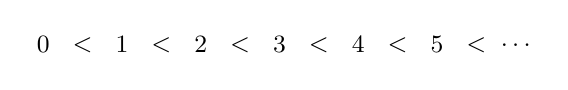
\begin{tikzpicture}
	\foreach \x/\xtext in {0, 1, 2, 3, 4, 5}
	{
		\node (\x a) at (\x, 1) {\small{$\x$}};
		\node (\x a) at (\x.5, 1) {\small{$<$}};
	}
	\node (ldots) at (6, 1) {\small{$\ldots$}};
	\end{tikzpicture}
\end{center}
પરિભાષામાં આપણે આને $\omega$-અનુક્રમ કહીએ છીએ.
ખરેખર, ગણોના પદાનુક્રમના તબક્કાઓની આપણી શરૂઆતની
રચનામાં પણ આ સામાન્ય ક્રમ પ્રતિબિંબિત થાય છે.
પણ હવે ધારો કે $0$ને આ અનુક્રમના અંતે મૂકીએ,
એટલે તે બીજી બધી સંખ્યાઓ પછી આવે:
\begin{center}
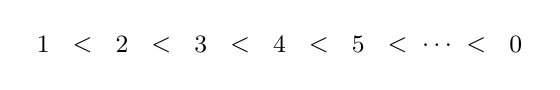
\begin{tikzpicture}
	\foreach \x/\xtext in {1, 2, 3, 4, 5}
	{
		\node (\x a) at (\x, 1) {\small{$\x$}};
		\node (\x a) at (\x.5, 1) {\small{$<$}};
	}
	\node (ldots) at (6, 1) {\small{$\ldots$}};
	\node (bea) at (6.5, 1) {\small{$<$}};
	\node (noa) at (7, 1) {\small{$0$}};
	\end{tikzpicture}
\end{center}
અહીં વસ્તુઓ એ જ છે, પણ તેમનો ક્રમ મૂળભૂત રીતે જુદો
છે: પહેલા ક્રમમાં અંતિમ ઘટક નહોતો; નવા ક્રમમાં છે.
ખરેખર, નવા ક્રમમાં વસ્તુઓનો $\omega$-અનુક્રમ
($1, 2, 3, 4, 5, \ldots$) આવે છે અને પછી બીજી
એક વસ્તુ આવે છે. આ $\omega+1$-અનુક્રમ થશે.

માત્ર આ જ વસ્તુઓથી ક્રમના વધુ પ્રકારો બનાવી શકીએ.
ઉદાહરણ તરીકે, બધી બેકી સંખ્યાઓ (તેમના સ્વાભાવિક
ક્રમમાં), અને પછી બધી એકી સંખ્યાઓ (તેમના સ્વાભાવિક
ક્રમમાં) વિચારો:
\begin{center}
\begin{tikzpicture}
	\node(a1) at (1,1) {\small{$0$}};
	\node(a2) at (1.5,1) {\small{$<$}};
	\node(a3) at (2,1) {\small{$2$}};
	\node(a4) at (2.5,1) {\small{$<$}};
	\node(a5) at (3,1) {\small{$4$}};
	\node(a6) at (3.5,1) {\small{$<$}};
	\node(dots) at (4,1) {\small{$\ldots$}};
	\node(aaoe) at (4.5,1) {\small{$<$}};
	\node(b1) at (5,1) {\small{$1$}};
	\node(b2) at (5.5,1) {\small{$<$}};
	\node(b3) at (6,1) {\small{$3$}};
	\node(b4) at (6.5,1) {\small{$<$}};
	\node(b5) at (7,1) {\small{$\ldots$}};
	\end{tikzpicture}
\end{center}
આ એક $\omega$-અનુક્રમ પછી બીજો $\omega$-અનુક્રમ
છે; એટલે $\omega+\omega$-અનુક્રમ.

આમ આપણે આગળ વધતા રહી શકીએ. પણ \emph{ક્રમો}
વિશેની આ વાતને સમજવાની એક સામાન્ય રીત જોઈએ છે.
% END OLP-0549
\endgroup

\begingroup
\makeatletter\def\ol@sectioncs{section}\makeatother

% BEGIN OLP-0550
\olfileid{sth}{ordinals}{wo}
\olsection{સુક્રમો}
\phantomsection\label{guunit:OLP-0550}


મૂળભૂત ખ્યાલ આ છે:

\begin{defn}
સંબંધ $<$ એ $A$ને \emph{સુક્રમિત} કરે જો અને ફક્ત જો નીચેની
બે શરતો પૂરી થાય:
\begin{enumerate}
	\item $<$ તુલનાયુક્ત છે, એટલે કે બધા $a, b \in A$ માટે
	કાં $a < b$ અથવા $a = b$ અથવા $b < a$;
	\item $A$ના દરેક અરિક્ત ઉપગણને $<$ મુજબ ન્યૂનતમ ઘટક
	હોય, એટલે કે જો $\emptyset \neq X \subseteq A$ તો
	$(\exists m \in
	X)(\forall z \in X)z \nless m$
\end{enumerate}
\end{defn}

હમણાં વિચારેલા ત્રણેય દાખલા ખરેખર સુક્રમિત કરનારા સંબંધો છે
તે સહેલાઈથી જોઈ શકાય છે.

\begin{prob}
\Olref[sth][ordinals][idea]{sec}માં પ્રાકૃતિક સંખ્યાઓ પરના
ત્રણ ક્રમોના દાખલા આપ્યા હતા. દરેક સુક્રમ છે તે તપાસો.
\end{prob}

સુક્રમ વિશેનાં કેટલાંક પ્રાથમિક પણ અત્યંત મહત્ત્વનાં અવલોકનો આ છે.

\begin{prop}\ollabel{wo:strictorder}
જો $<$ એ $A$ને સુક્રમિત કરતો હોય, તો $A$ના દરેક અરિક્ત
ઉપગણને અનન્ય $<$ મુજબ લઘુતમ સભ્ય હોય, અને $<$ અસ્વવાચક,
અસંમિત તથા પરંપરિત હોય.
\end{prop}

\begin{proof}
જો $X$ એ $A$નો અરિક્ત ઉપગણ હોય, તો તેને $<$ મુજબ
ન્યૂનતમ ઘટક $m$ હોય, એટલે કે
$(\forall z \in X)z \nless m$.
$<$ તુલનાયુક્ત હોવાથી $(\forall z \in X)m \leq z$.
તેથી $m$ એ $X$નો $<$ મુજબ લઘુતમ ઘટક છે.

અસ્વવાચકતા માટે કોઈ $a \in A$ લો; $\{a\}$નો $<$ મુજબ
લઘુતમ ઘટક $a$ છે, તેથી $a \nless a$.
પરંપરિતતા માટે, જો $a < b < c$, તો
$\{a, b, c\}$ને $<$ મુજબ લઘુતમ ઘટક હોવાથી
$a < c$. અસંમિતતા અસ્વવાચકતા અને પરંપરિતતાથી
મળે છે.
\end{proof}

\begin{prop}\ollabel{propwoinduction}
જો $<$ એ $A$ને સુક્રમિત કરતો હોય, તો કોઈ પણ સૂત્ર
$\phi(x)$ માટે:
\[
	\text{જો }(\forall a \in A)((\forall b < a)\phi(b) \lif
		\phi(a))\text{, તો }(\forall a \in A)\phi(a).
\]
\end{prop}

\begin{proof}
આપણે પ્રતિવિધાન સાબિત કરીશું. ધારો કે $\lnot(\forall a \in
A)\phi(a)$, એટલે કે $X = \Setabs{x \in A}{\lnot\phi(x)} \neq
\emptyset$. ત્યારે $X$ને $<$ મુજબ ન્યૂનતમ ઘટક $a$
હોય. તેથી $(\forall
b < a)\phi(b)$, પરંતુ $\lnot \phi(a)$.
\end{proof}\noindent આ છેલ્લા ગુણધર્મથી પ્રાકૃતિક સંખ્યાઓ પરના
પ્રબળ ગાણિતિક અનુમાનનો સિદ્ધાંત યાદ આવવો જોઈએ, એટલે કે:
જો $(\forall n \in \omega)((\forall m < n)\phi(m)
\lif \phi(n))$ હોય, તો $(\forall n \in \omega)\phi(n)$.
આ ગુણધર્મ સુક્રમને ખૂબ \emph{મજબૂત} ખ્યાલ બનાવે છે.\footnote{
યાદ રાખો: સ્પષ્ટપણે વિરુદ્ધ ન કહ્યું હોય તો બધા સૂત્રોમાં
પ્રાચલો હોઈ શકે છે.}
% END OLP-0550
\endgroup

\begingroup
\makeatletter\def\ol@sectioncs{section}\makeatother

% BEGIN OLP-0551
\olfileid{sth}{ordinals}{iso}
\olsection{ક્રમ-એકરૂપતાઓ}
\phantomsection\label{guunit:OLP-0551}


સુક્રમ \emph{કઈ રીતે} મજબૂત ખ્યાલ છે તે સમજાવવા માટે
સુક્રમોની સરખામણી કરવાની એક રીત રજૂ કરીને શરૂ કરીએ.

\begin{defn}
\emph{સુક્રમ} એવો જોડ $\tuple{A, <}$ છે કે $<$ એ $A$ને
સુક્રમિત કરે. સુક્રમો $\tuple{A, <}$ અને $\tuple{B,
\lessdot}$ \emph{ક્રમ-એકરૂપ} હોય જો અને ફક્ત જો એવું
એક-એક વ્યાપ્ત વિધેય $f \colon A \to B$ હોય કે:
$x < y$ તો અને ફક્ત તો $f(x) \lessdot  f(y)$.
આ કિસ્સામાં આપણે
$\ordeq{\tuple{A, <}}{\tuple{B, \lessdot}}$ લખીએ છીએ,
અને $f$ને \emph{ક્રમ-એકરૂપતા} કહીએ છીએ.
\end{defn}
\noindent
આગળ સંક્ષેપમાં આપણે “ક્રમ-એકરૂપતાઓ”ને બદલે “એકરૂપતાઓ”
કહીશું. સહજ રીતે, એકરૂપતાઓ એ સંરચના જાળવનારાં
એક-એક વ્યાપ્ત વિધેયો છે. એકરૂપતાઓ વિશેની કેટલીક સરળ હકીકતો આ છે.

\begin{lem}\ollabel{isoscompose}
એકરૂપતાઓનાં સંયોજનો એકરૂપતાઓ છે; એટલે કે:
જો $f \colon A
\to B$ અને $g \colon B \to C$ એકરૂપતાઓ હોય,
તો $(g \circ f)
\colon A \to C$ પણ એકરૂપતા છે.
\end{lem}
\begin{prob}
	\olref[sth][ordinals][iso]{isoscompose} સાબિત કરો.
\end{prob}
\begin{proof}
સ્વાધ્યાય તરીકે છોડ્યું છે.
\end{proof}
\begin{cor}\ollabel{ordisoisequiv}
	$\ordeq{X}{Y}$ એ સામ્ય સંબંધ છે.
\end{cor}
\begin{prop}\ollabel{ordisounique}
જો $\tuple{A, <}$ અને $\tuple{B, \lessdot}$ એકરૂપ સુક્રમો હોય,
તો તેમની વચ્ચેની એકરૂપતા અનન્ય છે.
\end{prop}

\begin{proof}
$f$ અને $g$ એ $A \to B$ એકરૂપતાઓ છે એમ લો.
પરિણામ \olref[wo]{propwoinduction} વાપરીને અનુમાનથી
સાબિત કરીશું.
કોઈ $a\in A$ લો, અને (અનુમાન માટે)
$(\forall b < a)f(b) = g(b)$ ધારો. કોઈ $x \in B$ લો.

જો $x \lessdot f(a)$ હોય, તો $f^{-1}(x) < a$,
તેથી $f$ અને $g$ એકરૂપતાઓ છે એથી
$g(f^{-1}(x)) \lessdot
g(a)$. પણ $f^{-1}(x) < a$ હોવાથી, આપણી ધારણા મુજબ
$x =f(f^{-1}(x)) = g(f^{-1}(x))$.
આમ $x \lessdot g(a)$. એ જ રીતે, જો
$x \lessdot g(a)$ હોય, તો $x \lessdot f(a)$.

સામાન્ય રીતે,
$(\forall x \in B)(x \lessdot f(a) \liff x \lessdot
g(a))$. તેથી
\olref[sfr][rel][ord]{prop:extensionality-strictlinearorders}
મુજબ $f(a) = g(a)$. આમ
\olref[wo]{propwoinduction}થી
$(\forall
a \in A)f(a) = g(a)$.
\end{proof}\noindent
આથી સુક્રમો મજબૂત ખ્યાલ કેમ છે તેનો થોડો ખ્યાલ મળે છે.
પણ આ વાત આગળ સમજાવવા માટે થોડા વધુ સંકેતો ઉપયોગી થશે.

\begin{defn}
જ્યારે $\tuple{A, <}$ સુક્રમ હોય અને $a \in A$ હોય, ત્યારે
$A_a = \Setabs{x \in A}{x
< a}$ લો. $A_a$ને $A$નો ઉચિત \emph{આરંભિક ખંડ} કહીએ
છીએ (અને $A$ પોતે પણ $A$નો અનુચિત આરંભિક ખંડ છે એમ માનીએ છીએ).
$<_a$ એ આરંભિક ખંડ પર $<$નું મર્યાદન છે, એટલે કે
$\funrestrictionto{\mathord{<}}{A_a^2}$.
\end{defn}
\noindent
આ સંકેતો વડે કહી અને સાબિત કરી શકીએ છીએ કે કોઈ સુક્રમ
પોતાના કોઈ ઉચિત આરંભિક ખંડ સાથે એકરૂપ નથી.

\begin{lem}\ollabel{wellordnotinitial}
જો $\tuple{A, <}$ સુક્રમ હોય અને $a \in A$ હોય, તો
$\ordneq{\tuple{A, <}}{\tuple{A_a, <_a}}$
\end{lem}

\begin{proof}
વિરોધાભાસ માટે ધારો કે $f \colon A \to A_a$ એકરૂપતા
છે. $f$ એ દ્વિએક વિધેય છે અને $A_a \subsetneq A$,
તેથી \olref[wo]{wo:strictorder} વાપરીને
$A$માં એવો $<$ મુજબ લઘુતમ ઘટક $b \in A$ લો
કે $b \neq f(b)$. આપણે
$(\forall x \in A)(x<b \liff x < f(b))$ બતાવીશું;
પછી
\olref[sfr][rel][ord]{prop:extensionality-strictlinearorders}
મુજબ $b =
f(b)$ મળશે અને વિરોધાભાસ પૂર્ણ થશે.

ધારો કે $x < b$. $b$ની પસંદગી મુજબ $x = f(x)$.
વળી $f$ એકરૂપતા હોવાથી $f(x) <
f(b)$. તેથી $x < f(b)$.

ધારો કે $x < f(b)$. $f$ એકરૂપતા હોવાથી
$f^{-1}(x) < b$, અને તેથી $b$ની પસંદગી મુજબ
$f^{-1}(x) = x$. આમ $x < b$.
\end{proof}

આગળનું પરિણામ લગભગ એમ કહે છે કે એકરૂપતાનો
“આરંભિક ખંડ” પણ એકરૂપતા છે:

\begin{lem}\ollabel{wellordinitialsegment}
$\tuple{A, <}$ અને $\tuple{B, \lessdot}$ સુક્રમો હોય.
જો $f
\colon A \to B$ એકરૂપતા હોય અને $a \in A$ હોય,
તો $\funrestrictionto{f}{A_{a}} : A_a \to B_{f(a)}$
એકરૂપતા છે.
\end{lem}

\begin{proof}
$f$ એકરૂપતા હોવાથી:
\begin{align*}
	\funimage{f}{A_a} &= \funimage{f}{\Setabs{x \in A}{x < a}}\\
	&= \funimage{f}{\Setabs{f^{-1}(y) \in A}{f^{-1}(y) < a}} \\
	&= \Setabs{y \in B}{y \lessdot f(a)} \\
	&=B_{f(a)} 
\end{align*}
અને $\funrestrictionto{f}{A_a}$ ક્રમ જાળવે છે,
કારણ કે $f$ ક્રમ જાળવે છે.
\end{proof}

આગળનાં બે પરિણામો બતાવે છે કે સુક્રમોની હંમેશાં
સરખામણી થઈ શકે છે:

\begin{lem}\ollabel{lemordsegments}
$\tuple{A, <}$ અને $\tuple{B, \lessdot}$ સુક્રમો હોય.
જો
$\ordeq{\tuple{A_{a_1}, <_{a_1}}}{\tuple{B_{b_1}, \lessdot_{b_1}}}$
અને
$\ordeq{\tuple{A_{{a_2}}, <_{a_2}}}{\tuple{B_{{b_2}},
\lessdot_{b_2}}}$ હોય, તો
$ {a_1}  < {a_2} \text{ તો અને ફક્ત તો }{b_1} \lessdot
{b_2}$.
\end{lem}

\begin{proof}
આપણે \emph{ડાબેથી જમણી તરફ} સાબિત કરીશું;
બીજી દિશાની દલીલ એવી જ છે.
ધારો કે
$\ordeq{\tuple{A_{a_1}, <_{a_1}}}{\tuple{B_{b_1},
\lessdot_{b_1}}}$ અને
$\ordeq{\tuple{A_{{a_2}},
<_{a_2}}}{\tuple{B_{{b_2}}, \lessdot_{b_2}}}$ બંને છે,
અને $f \colon
A_{{a_2}} \to B_{{b_2}}$ આપણી એકરૂપતા છે.
$ {a_1} < {a_2}$ લો; ત્યારે
\olref{wellordinitialsegment}થી
$\ordeq{\tuple{A_{a_1}, <_{a_1}}}{\tuple{B_{f({a_1})},
\lessdot_{f({a_1})}}}$.
તેથી
$\ordeq{\tuple{B_{b_1}, \lessdot_{b_1}}}{\tuple{B_{f({a_1})},
\lessdot_{f({a_1})}}}$, અને આમ
\olref{wellordnotinitial}થી
$ {b_1} = f({a_1})$.
હવે $f$નો સહપ્રદેશ $B_{{b_2}}$ હોવાથી
$ {b_1} \lessdot {b_2}$.
\sourcecorrection{OLMD-115}{મૂળના આ પગલામાં $f$નો
“પ્રદેશ” $B_{{b_2}}$ કહેવાયો છે; પરંતુ ઉપર
$f\colon A_{{a_2}}\to B_{{b_2}}$ છે. અહીં
$B_{{b_2}}$ એ $f$નો સહપ્રદેશ (અને એકરૂપતા હોવાથી
વિસ્તાર) છે. આ પ્રકારે જ $b_1$ એ $b_2$થી
નાનો હોવાનું ફલિત થાય છે.}
\end{proof}

\begin{thm}\ollabel{thm:woalwayscomparable}
કોઈ પણ બે સુક્રમો આપેલા હોય, તો એક સુક્રમ બીજાના
કોઈ આરંભિક ખંડ (ઉચિત હોવો જરૂરી નથી) સાથે એકરૂપ હોય છે.
\end{thm}

\begin{proof}
$\tuple{A, <}$ અને $\tuple{B, \lessdot}$ સુક્રમો
હોય. પૃથક્કરણ વાપરીને લો
\[
	f = \Setabs{\tuple{a, b} \in A \times B}{
		\ordeq{\tuple{A_a, <_a}}{\tuple{B_b, \lessdot_b}}}.
\]
\olref{lemordsegments} મુજબ બધા
$\tuple{a_1, b_1}, \tuple{a_2, b_2} \in f$ માટે
$a_1 < a_2$ તો અને ફક્ત તો
$b_1 \lessdot b_2$. તેથી
$f \colon \dom{f} \to
\ran{f}$ એકરૂપતા છે.

જો $a_2 \in \dom{f}$ અને $a_1 < a_2$ હોય, તો
\olref{wellordinitialsegment}થી
$a_1 \in \dom{f}$; એટલે $\dom{f}$ એ $A$નો
આરંભિક ખંડ છે. એ જ રીતે, $\ran{f}$ એ $B$નો
આરંભિક ખંડ છે. વિરોધાભાસ માટે ધારો કે બંને
\emph{ઉચિત} આરંભિક ખંડ છે. ત્યારે $a$ એ
$A \setminus \dom{f}$નો $<$ મુજબ લઘુતમ
ઘટક હોય એવું લો, જેથી $\dom{f} =
A_a$; અને $b$ એ
$B \setminus
\ran{f}$નો $\lessdot$ મુજબ લઘુતમ
ઘટક હોય એવું લો, જેથી
$\ran{f} = B_b$. આમ
$f \colon A_a \to B_b$ એકરૂપતા છે અને તેથી
$\tuple{a, b} \in f$, જે વિરોધાભાસ છે.
\end{proof}
% END OLP-0551
\endgroup

\begingroup
\makeatletter\def\ol@sectioncs{section}\makeatother

% BEGIN OLP-0552
\olfileid{sth}{ordinals}{vn}
\olsection[વૉન નોયમનની રચના]{વૉન નોયમનની ક્રમવાચક સંખ્યાઓની રચના}
\phantomsection\label{guunit:OLP-0552}


\olref[sth][ordinals][iso]{thm:woalwayscomparable}થી એક વિચાર
સૂઝે છે. સુક્રમોના અવેજ તરીકે કામ કરવા માટે
\emph{ક્રમપ્રકારો} કહેવાતી અમુક વસ્તુઓ રજૂ કરી શકીએ.
સુક્રમ $\tuple{A, <}$ના ક્રમપ્રકાર માટે
$\ordtype{A, <}$ લખીએ, તો નીચેના બે સિદ્ધાંતો મળે
એવી આશા રાખીએ:
\begin{align*}
	\ordtype{A, <} = \ordtype{B, \lessdot} &
	\text{ તો અને ફક્ત તો } \ordeq{\tuple{A, <}}{\tuple{B, \lessdot}}\\
	\ordtype{A, <} < \ordtype{B, \lessdot}&
	\text{ તો અને ફક્ત તો }\ordeq{\tuple{A, <}}{\tuple{B_b, \lessdot_b}}\text{ જ્યાં કોઈ }b \in B
\end{align*}
વધુમાં, જેમ પ્રાકૃતિક સંખ્યાઓને અમુક ગણો તરીકે રજૂ
કરી શકીએ છીએ, તેમ ક્રમપ્રકારોને પણ \emph{અમુક ગણો
તરીકે} રજૂ કરી શકીએ એવી આશા રાખીએ.

આવું કરવાની સૌથી સામાન્ય રીત---અને આપણે અનુસરવાની
રીત---એ આ ક્રમપ્રકારોને અમુક \emph{પ્રમાણભૂત} સુક્રમિત
ગણો દ્વારા વ્યાખ્યાયિત કરવાની છે. આ પ્રમાણભૂત ગણો
સૌપ્રથમ વૉન નોયમને રજૂ કર્યા:

\begin{defn}
ગણ $A$ \emph{પરંપરિત} હોય જો અને ફક્ત જો
$(\forall x \in A)x \subseteq
A$. પછી $A$ એ \emph{ક્રમવાચક સંખ્યા} હોય જો અને ફક્ત
જો $A$ પરંપરિત હોય અને $\in$ વડે સુક્રમિત હોય.
\end{defn}
\noindent
આગળ ક્રમવાચક સંખ્યાઓ માટે ગ્રીક અક્ષરો વાપરીશું.
વ્યાખ્યાથી સીધું મળે છે કે જો $\alpha$ ક્રમવાચક
સંખ્યા હોય, તો $\tuple{\alpha, \in_\alpha}$
સુક્રમ છે, જ્યાં $\in_\alpha =
\Setabs{\tuple{x, y} \in \alpha^2}{x \in y}$.
તેથી સંકેતનો થોડો છૂટો ઉપયોગ કરીને આપણે કહી
શકીએ કે $\alpha$ \emph{પોતે} સુક્રમ છે.

આપણી શરૂઆતની કેટલીક ક્રમવાચક સંખ્યાઓ આ છે:
\[
	\emptyset, \{\emptyset\},
	\{\emptyset, \{\emptyset\}\},
	\{\emptyset, \{\emptyset\}, \{\emptyset, \{\emptyset\}\}\}, \ldots
\]
તમે નોંધશો કે આ જ કેટલીક શરૂઆતની ક્રમવાચક
સંખ્યાઓ અનંતતાની સ્વયંસિદ્ધિમાં, એટલે કે વૉન
નોયમનની $\omega$ની વ્યાખ્યામાં, મળી હતી
(\olref[sth][z][infinity-again]{sec} જુઓ).
આ કોઈ યોગાનુયોગ નથી. વૉન નોયમનની ક્રમવાચક
સંખ્યાઓની વ્યાખ્યા પ્રાકૃતિક સંખ્યાઓને ક્રમવાચક
સંખ્યાઓ તરીકે લે છે, પણ અનંતાતીત ક્રમવાચક
સંખ્યાઓને પણ સ્થાન આપે છે.

હંમેશની જેમ હવે પૂછી શકીએ: શું આ જ ક્રમવાચક
સંખ્યાઓ \emph{છે}? કે વૉન નોયમને ફક્ત એવા
કેટલાક ગણો આપ્યા છે જેને આપણે ક્રમવાચક
સંખ્યાઓ \emph{તરીકે લઈ} શકીએ?
આ પ્રશ્ન અંગેની ચર્ચા
\olref[sfr][rel][ref]{sec},
\olref[sfr][arith][ref]{sec},
\olref[sfr][infinite][dedekindsproof]{sec} અને
\olref[sth][z][nat]{sec}માં થયેલી ચર્ચાઓ જેવી
જ હશે; તેથી ફરી વિસ્તાર નહીં કરીએ.
આગળ “ક્રમવાચક સંખ્યાઓ”નો અર્થ માત્ર “વૉન
નોયમનની ક્રમવાચક સંખ્યાઓ” જ લઈશું.
% END OLP-0552
\endgroup

\begingroup
\makeatletter\def\ol@sectioncs{section}\makeatother

% BEGIN OLP-0553
\olfileid{sth}{ordinals}{basic}
\olsection{ક્રમવાચક સંખ્યાઓના મૂળભૂત ગુણધર્મો}
\phantomsection\label{guunit:OLP-0553}


આપણે જોયું કે શરૂઆતની કેટલીક ક્રમવાચક સંખ્યાઓ
પ્રાકૃતિક સંખ્યાઓ જ છે. ક્રમવાચક સંખ્યાઓનો સિદ્ધાંત
વિકસાવવાનું મુખ્ય કારણ પ્રાકૃતિક સંખ્યાઓ પર સાચા
અનુમાનના સિદ્ધાંતને આગળ વિસ્તારવાનું છે. પ્રાથમિક
પરિણામોની શ્રેણીથી આપણે ત્યાં સુધી પહોંચીશું.

\begin{lem}\ollabel{ordmemberord}
ક્રમવાચક સંખ્યાનો દરેક ઘટક પણ ક્રમવાચક
સંખ્યા છે.
\end{lem}

\begin{proof}
$\alpha$ ક્રમવાચક સંખ્યા હોય અને $b \in \alpha$ હોય.
$\alpha$ પરંપરિત હોવાથી $b \subseteq \alpha$.
તેથી $\in$ એ $b$ને સુક્રમિત કરે છે, કારણ કે
$\in$ એ $\alpha$ને સુક્રમિત કરે છે.

$b$ પરંપરિત છે તે જોવા માટે ધારો કે $x \in c \in b$.
$b
\subseteq \alpha$ હોવાથી $c \in \alpha$.
ફરી $\alpha$ પરંપરિત હોવાથી $c \subseteq
\alpha$, એટલે $x \in \alpha$.
આમ $x, c, b \in \alpha$.
પણ $\in$ એ $\alpha$ને સુક્રમિત કરે છે, તેથી
\olref[sth][ordinals][wo]{wo:strictorder} મુજબ
$\alpha$ પરનો $\in$ સંબંધ પરંપરિત છે.
એટલે $x
\in c \in b$ હોવાથી $x \in b$.
સામાન્ય રીતે, $c \subseteq b$.
\end{proof}

\begin{cor}\ollabel{ordissetofsmallerord}
કોઈ પણ ક્રમવાચક સંખ્યા~$\alpha$ માટે
$\alpha = \Setabs{\beta \in \alpha}{\beta \text{ ક્રમવાચક સંખ્યા છે}}$.
\end{cor}

\begin{proof}
\olref{ordmemberord}થી સીધું મળે છે.
\end{proof}

આગળનાં બે મુખ્ય પરિણામો,
\olref{ordinductionschema} અને
\olref{ordtrichotomy}, આશરે એ કહે છે કે
ક્રમવાચક સંખ્યાઓ પોતે સભ્યતા-સંબંધથી સુક્રમિત છે:

\begin{thm}[અનંતાતીત અનુમાન]\ollabel{ordinductionschema}
કોઈ પણ સૂત્ર $\phi(x)$ માટે:
\[
	\text{જો }\exists \alpha \phi(\alpha)\text{, તો }\exists \alpha(\phi(\alpha)
	\land  (\forall \beta \in \alpha) \lnot \phi(\beta))
\]
અહીં દર્શાવેલા પરિમાણકો પરોક્ષ રીતે ક્રમવાચક
સંખ્યાઓ સુધી મર્યાદિત છે.
\end{thm}

\begin{proof}
ધારો કે કોઈ ક્રમવાચક સંખ્યા $\alpha$ માટે
$\phi(\alpha)$ છે. જો
$ (\forall \beta
\in \alpha) \lnot \phi(\beta)$ હોય, તો કામ પૂરું.
નહિતર $\alpha$ના એવા સભ્યોમાંથી, જેમના માટે
$\phi$ સાચું છે, $\in$ મુજબ લઘુતમ ઘટક
પસંદ કરો. આપેલો ગણ ક્રમવાચક સંખ્યા હોવાથી
આવો સભ્ય છે અને તે \olref{ordmemberord}
મુજબ ક્રમવાચક સંખ્યા પણ છે.
\sourcecorrection{OLMD-116}{મૂળમાં માત્ર $\alpha$ને
કોઈ $\in$-લઘુતમ સભ્ય છે “જે $\phi$ છે”
એમ કહેવાયું છે. જરૂરી પસંદગી આખા $\alpha$માંથી
નહીં, પણ $\phi$ સંતોષતા તેના સભ્યોના અરિક્ત
ઉપગણમાંથી કરવી પડે: પહેલેથી $\phi(\alpha)$
હોય અને તે ઉપગણ ખાલી હોય તો $\alpha$ સાક્ષી છે;
નહિતર ઉપગણનો લઘુતમ સભ્ય સાક્ષી છે.}
\end{proof}
\noindent
નોંધો કે \olref{ordinductionschema}ને સમકક્ષ રીતે
આ પ્રરૂપ તરીકે પણ વ્યક્ત કરી શકાય:
\[
\text{જો }\forall \alpha((\forall \beta \in \alpha)\phi(\beta) \lif
\phi(\alpha))\text{, તો }\forall \alpha\phi(\alpha)
\]
\olref{ordinductionschema}માં
$\lnot\phi(\alpha)$ મૂકીને અને પછી પ્રાથમિક
તાર્કિક ફેરફારો કરીને આ મળે છે.

\begin{thm}[ત્રિવિકલ્પતા]\ollabel{ordtrichotomy}
કોઈ પણ ક્રમવાચક સંખ્યાઓ $\alpha$ અને $\beta$ માટે
$\alpha \in \beta \lor \alpha = \beta \lor \beta \in \alpha$.
\end{thm}

\begin{proof}
સાબિતી બે વાર અનુમાનથી છે, એટલે કે
\olref{ordinductionschema} બે વાર વાપરીશું.
$x$ એ $y$ સાથે \emph{તુલનીય} છે એમ કહીએ
જો અને ફક્ત જો
$x \in y \lor x = y \lor y \in x$.

અનુમાન માટે ધારો કે~$\alpha$માંની દરેક
ક્રમવાચક સંખ્યા \emph{દરેક} ક્રમવાચક
સંખ્યા સાથે તુલનીય છે.
બીજા અનુમાન માટે ધારો કે
$\alpha$ એ~$\beta$માંની દરેક ક્રમવાચક
સંખ્યા સાથે તુલનીય છે.
આપણે $\alpha$ અને~$\beta$ તુલનીય છે તે
બતાવીશું. પછી~$\beta$ પરના અનુમાનથી
$\alpha$ દરેક ક્રમવાચક સંખ્યા સાથે
તુલનીય છે; અને ત્યાર બાદ~$\alpha$ પરના
અનુમાનથી \emph{દરેક} ક્રમવાચક સંખ્યા
\emph{દરેક} ક્રમવાચક સંખ્યા સાથે તુલનીય
છે, જેમ જોઈએ છે.
$\alpha \notin \beta$ અને
$\beta \notin
\alpha$ ધારીને $\alpha = \beta$ બતાવવું પૂરતું છે.

$\alpha \subseteq \beta$ બતાવવા કોઈ
$\gamma \in \alpha$ લો; \olref{ordmemberord}
મુજબ તે ક્રમવાચક સંખ્યા છે.
તેથી પહેલી અનુમાન-ધારણા મુજબ
$\gamma$ એ $\beta$ સાથે તુલનીય છે.
પણ જો $\gamma
= \beta$ અથવા $\beta \in \gamma$ હોય,
તો (જરૂર પડે ત્યાં $\alpha$ પરંપરિત છે તે
વાપરીને) $\beta \in \alpha$ થશે, જે
આપણી ધારણાની વિરુદ્ધ છે; તેથી
$\gamma \in \beta$. સામાન્ય રીતે,
$\alpha \subseteq
\beta$.

એ જ પ્રકારની દલીલ બીજી અનુમાન-ધારણા
વાપરીને $\beta \subseteq \alpha$ બતાવે છે.
તેથી $\alpha = \beta$.
\end{proof}\noindent તેથી આપણે ક્યારેક
$\alpha \in \beta$ને બદલે $\alpha <\beta$
લખીશું, કારણ કે $\in$ અહીં ક્રમસંબંધ
જેવો વ્યવહાર કરે છે. પરિચિતપણું અને
$\alpha \in
\beta \lor \alpha = \beta$ કરતાં
$\alpha \leq \beta$ લખવું સરળ હોવું
એ સિવાય આ માટે કોઈ ગહન કારણ નથી.\footnote{
આપણે $\alpha
\mathrel{\underline{\in}} \beta$ લખી શકીએ,
પણ તે તદ્દન અપ્રચલિત સંકેત થશે.}

આ છેલ્લાં પરિણામોનાં બે ટૂંકાં ફલિતાર્થો
આ છે; પહેલું આપણા નવા સંકેતનો ઉપયોગ કરે છે:

\begin{cor}\ollabel{ordordered}
જો $\exists \alpha\phi(\alpha)$ હોય, તો
$\exists \alpha(\phi(\alpha)
\land \forall \beta(\phi(\beta) \lif \alpha \leq \beta))$.
વધુમાં, કોઈ પણ ક્રમવાચક સંખ્યાઓ
$\alpha, \beta, \gamma$ માટે
$\alpha
\notin \alpha$ અને
$\alpha \in \beta \in \gamma \lif \alpha \in
\gamma$ બંને સાચાં છે.
\end{cor}

\begin{proof}
\olref[wo]{wo:strictorder} જેવી જ દલીલ.
\end{proof}

\begin{prob}
\olref[sth][ordinals][basic]{ordtrichotomy}ની
સાબિતીમાં “એ જ પ્રકારની દલીલ” પૂરી કરો.
\end{prob}

\begin{cor}\ollabel{corordtransitiveord}
$A$ ક્રમવાચક સંખ્યા હોય જો અને ફક્ત જો
$A$ એ ક્રમવાચક સંખ્યાઓનો પરંપરિત ગણ હોય.
\end{cor}

\begin{proof}
\emph{ડાબેથી જમણે.} \olref{ordmemberord} મુજબ.
\emph{જમણેથી ડાબે.}
જો $A$ ક્રમવાચક સંખ્યાઓનો પરંપરિત
ગણ હોય, તો
\olref{ordinductionschema} અને
\olref{ordtrichotomy} મુજબ
$\in$ એ $A$ને સુક્રમિત કરે છે.
\end{proof}

હમણાં આપણે \olref{ordinductionschema}
અને \olref{ordtrichotomy}નો સાર એ રીતે
કહ્યો કે $\in$ ક્રમવાચક સંખ્યાઓને
સુક્રમિત કરે છે. જોકે આગળના પરિણામને
લીધે આવા દાવા અંગે આપણે \emph{ખૂબ સાવચેત}
રહેવું જોઈએ:

\begin{thm}[બુરાલી–ફૉર્ટીનો વિરોધાભાસ]\ollabel{buraliforti}
બધી ક્રમવાચક સંખ્યાઓનો ગણ નથી.
\end{thm}

\begin{proof}
વિરોધાભાસ માટે ધારો કે $O$ બધી
ક્રમવાચક સંખ્યાઓનો ગણ છે.
જો $\alpha \in
\beta \in O$ હોય, તો
\olref{ordmemberord} મુજબ $\alpha$
ક્રમવાચક સંખ્યા છે, તેથી
$\alpha \in O$.
આમ $O$ પરંપરિત છે અને તેથી
\olref{corordtransitiveord} મુજબ
$O$ ક્રમવાચક સંખ્યા છે.
એટલે $O \in O$, જે
\olref{ordordered} સાથે વિરોધાભાસ કરે છે.
\end{proof}
\noindent
આ પરિણામનું નામ \citeauthor{Burali-Forti1897}
પરથી પડ્યું છે. પરંતુ 1899માં ડેડેકિન્ડને
લખેલા પત્રમાં કૅન્ટૉરે બધી ક્રમવાચક
સંખ્યાઓનો ગણ માનતાં ઊભો થતો
\emph{વિરોધાભાસ} પહેલી વાર સ્પષ્ટ રીતે
જોયો હતો. વાન હેયેનૉર્ટ સમજાવે છે તેમ:
\begin{quote}
  બુરાલી–ફૉર્ટીએ પોતે વિરોધાભાસને
  \emph{વિરોધાભાસ વડે સાબિતી}થી
  એવું પરિણામ મળ્યું હોવાનું માન્યું કે
  ક્રમવાચક સંખ્યાઓનો સ્વાભાવિક ક્રમ
  માત્ર આંશિક ક્રમ છે.
  \citep[p.~105]{Heijenoort1967}
\end{quote}
બુરાલી–ફૉર્ટીની ભૂલને બાજુએ રાખીને
અત્યાર સુધીની વાત આ રીતે કહી શકીએ:
ક્રમવાચક સંખ્યાઓ એવા ગણો છે જે
અલગ અલગ રીતે સભ્યતા-સંબંધથી
સુક્રમિત છે, અને સામૂહિક રીતે પણ
સભ્યતા-સંબંધથી સુક્રમિત છે
(પણ એ બધી મળીને ગણ બનતી નથી).

છેલ્લે, ક્રમવાચક સંખ્યાઓના
\olref{ordinductionschema} અને
\olref{ordtrichotomy}માંથી મળતાં
કેટલાક વધુ મૂળભૂત ગુણધર્મો આ છે.

\begin{prop}
ક્રમવાચક સંખ્યાઓનો કોઈ પણ કડક
ઊતરતો અનુક્રમ સાન્ત હોય છે.
\end{prop}

\begin{proof}
ક્રમવાચક સંખ્યાઓના કોઈ અનંત કડક
ઊતરતા અનુક્રમ
$\alpha_0 > \alpha_1 > \alpha_2 > \ldots$માં
$<$ મુજબ ન્યૂનતમ સભ્ય નથી;
આ \olref{ordinductionschema}ની
વિરુદ્ધ છે.
\end{proof}

\begin{prop}\ollabel{ordinalsaresubsets}
કોઈ પણ ક્રમવાચક સંખ્યાઓ
$\alpha, \beta$ માટે
$\alpha \subseteq \beta \lor \beta \subseteq \alpha$.
\end{prop}

\begin{proof}
જો $\alpha \in \beta$, તો $\beta$
પરંપરિત હોવાથી $\alpha \subseteq \beta$.
એ જ રીતે, જો $\beta \in \alpha$,
તો $\beta \subseteq
\alpha$. અને જો $\alpha = \beta$,
તો $\alpha \subseteq \beta$ અને
$\beta \subseteq \alpha$.
તેથી \olref{ordtrichotomy} મુજબ
દલીલ પૂરી થાય છે.
\end{proof}

\begin{prop}\ollabel{ordisoidentity}
કોઈ પણ ક્રમવાચક સંખ્યાઓ
$\alpha, \beta$ માટે
$\alpha = \beta$ તો અને ફક્ત તો
$\ordeq{\alpha}{\beta}$.
\end{prop}

\begin{proof}
ક્રમવાચક સંખ્યાઓ સુક્રમો છે;
તેથી ત્રિવિકલ્પતા
(\olref[basic]{ordtrichotomy}) અને
\olref[iso]{wellordnotinitial}થી
આ સીધું મળે છે.
\end{proof}

\begin{prob}\ollabel{probunionordinalsordinal}
જો $X$નો દરેક સભ્ય ક્રમવાચક
સંખ્યા હોય, તો $\bigcup X$
ક્રમવાચક સંખ્યા છે તે સાબિત કરો.
\end{prob}
% END OLP-0553
\endgroup

\begingroup
\makeatletter\def\ol@sectioncs{section}\makeatother

% BEGIN OLP-0554
\olfileid{sth}{ordinals}{replacement}
\olsection{પ્રતિસ્થાપન}
\phantomsection\label{guunit:OLP-0554}


\olref[sth][ordinals][vn]{sec}માં આપણે ક્રમવાચક સંખ્યાઓ રજૂ કરવા માટે
એવો વિચાર કર્યો હતો કે તેમને ક્રમપ્રકારો, એટલે કે સુક્રમોના પ્રમાણભૂત
અવેજો, તરીકે લઈ શકાય. આ વિચાર સફળ થવા માટે આપણે સાબિત કરવું પડે કે
\emph{દરેક સુક્રમ કોઈ ક્રમવાચક સંખ્યા સાથે ક્રમ-એકરૂપ છે}.
પછી $\tuple{A, <} \isomorphic \alpha$ થાય એવી ક્રમવાચક
સંખ્યા $\alpha$ તરીકે $\ordtype{A, <}$ વ્યાખ્યાયિત કરી શકીએ.

દુર્ભાગ્યે, અત્યાર સુધી રજૂ કરેલાં સ્વયંસિદ્ધિઓથી જ આપણે આ ઇચ્છિત
પરિણામ \emph{સાબિત કરી શકતા નથી}. તેનું કારણ
\olref[replacement][strength]{sec}માં જોઈશું; હાલ એટલું જાણવું
પૂરતું છે કે આ પરિણામ મળતું નથી. તેથી એક નવો વિચાર જોઈએ:

\begin{axiom}[પ્રતિસ્થાપનનું પ્રરૂપ]
કોઈ પણ સૂત્ર $\phi(x, y)$ માટે નીચેનું એક સ્વયંસિદ્ધિ છે:
\begin{quote}
	કોઈ પણ $A$ માટે, જો $(\forall x \in A)\lexists![y][\phi(x,y)]$ હોય, તો
	$\Setabs{y}{(\exists x \in A)\phi(x,y)}$ અસ્તિત્વમાં છે.
\end{quote}
\end{axiom}
\noindent
પૃથક્કરણની જેમ આ પણ પ્રરૂપ છે: જુદાં જુદાં અસંખ્ય $\phi$ સૂત્રોમાંથી
દરેક માટે તે એક સ્વયંસિદ્ધિ આપે છે. તેને સમકક્ષ રીતે, અને સામાન્ય રીતે,
આ પ્રમાણે પણ લખાય છે:

\begin{defish}
``$B$'' ન આવતું હોય એવા કોઈ પણ સૂત્ર $\phi(x,y)$ માટે નીચેનું એક સ્વયંસિદ્ધિ છે:
\[
\forall A[(\forall x \in A)\lexists![y][\phi(x,y)] \lif \exists B\forall y (y \in B \liff (\exists x \in A)\phi(x,y))]
\]
\end{defish}

જોકે, પહેલી વાર જોતાં આ સૂત્ર ગૂંચવણભર્યું લાગે છે. પ્રતિસ્થાપનનું
આગળનું તાત્કાલિક પરિણામ આપણે સમજવા માગીએ છીએ તે વિચારને કદાચ વધુ
\emph{સ્પષ્ટ રીતે} વ્યક્ત કરે છે:\footnote{પદ એવી અભિવ્યક્તિ છે
જે તેના મુક્ત ચલોને મૂલ્યો આપીએ ત્યારે બરાબર એક જ વસ્તુ નિર્દેશે છે.
દાખલા તરીકે, ``$\emptyset$'' ખાલી ગણને નિર્દેશતું પદ છે;
``$\{x\}$'' એ $x$ના એકઘટકી ગણને નિર્દેશતું પદ છે, ભલે $x$ ગમે તે હોય;
અને ``$x \cup y$'' એ $x$ અને $y$ના યોગગણને નિર્દેશતું પદ છે,
ભલે તેઓ ગમે તે હોય.}

\begin{cor}
કોઈ પણ પદ $\tau(x)$ અને કોઈ પણ ગણ $A$ માટે નીચેનો ગણ અસ્તિત્વમાં છે:
\[
	\Setabs{\tau(x)}{x \in A} = \Setabs{y}{(\exists x \in A)y = \tau(x)}.
\]
\end{cor}

\begin{proof}
$\tau$ \emph{પદ} હોવાથી $\forall x \lexists![y][\tau(x) = y]$.
તેથી ખાસ કરીને $(\forall x \in A)\lexists![y][\tau(x) = y]$.
આથી પ્રતિસ્થાપન મુજબ
$\Setabs{y}{(\exists x \in A)\tau(x) = y}$ અસ્તિત્વમાં છે.
\end{proof}
\noindent
આ પરથી ``પ્રતિસ્થાપન'' નામ યોગ્ય લાગે છે: આપેલા ગણ $A$ના દરેક સભ્યને
$\tau$ હેઠળ તેના પ્રતિબિંબથી બદલીને નવો ગણ
$\Setabs{\tau(x)}{x \in A}$ બનાવી શકાય છે. ખરેખર, કોઈ વિધેય
હેઠળ $A$ના પ્રતિબિંબ માટેના સંકેત મુજબ, $\Setabs{\tau(x)}{x \in A}$ને
$\funimage{\tau}{A}$ પણ લખી શકીએ.

પરંતુ અહીં મહત્ત્વનું એ છે કે $\tau$ એક \emph{પદ} છે. તે
\olref[sfr][fun][rel]{sec}ના અર્થમાં, એટલે કે ક્રમિત જોડીઓના
કોઈ ચોક્કસ ગણ તરીકે, \emph{વિધેય} હોવું જરૂરી નથી, અને તેનું નામ
હોવું પણ જરૂરી નથી. જો $f$ એ અર્થમાં વિધેય હોય, તો
$\funimage{f}{A} = \Setabs{f(x)}{x \in
A}$ એ માત્ર $\ran{f}$નો એક ઉપગણ છે. આ ઉપગણનું અસ્તિત્વ
તો $\Zminus$નાં સ્વયંસિદ્ધિઓથી જ મળે છે.\footnote{માત્ર
$\Setabs{y \in \bigcup \bigcup f}{(\exists x \in A)y =
f(x)}$ લો.} તેના મુકાબલે, પ્રતિસ્થાપન આપણા સ્વયંસિદ્ધિઓમાં
\emph{શક્તિશાળી} ઉમેરો છે, જે
\olref[sth][replacement][]{chap}માં જોઈશું.
% END OLP-0554
\endgroup

\begingroup
\makeatletter\def\ol@sectioncs{section}\makeatother

% BEGIN OLP-0555
\olfileid{sth}{ordinals}{zfm}	
\olsection{$\ZFminus$: એક મહત્ત્વનો પડાવ}
\phantomsection\label{guunit:OLP-0555}


પ્રતિસ્થાપનને કેવી રીતે વાજબી ઠેરવવું, અને ઠેરવી શકાય પણ ખરું કે
નહીં, તે પ્રશ્ન સરળ નથી. તેથી તેની ચર્ચા
\olref[replacement][]{chap} માટે રાખીશું. જોકે પ્રતિસ્થાપન
ઉમેરવાથી આપણે બીજો એક મહત્ત્વનો પડાવ પાર કર્યો છે. હવે સિદ્ધાંત
$\ZFminus$ માટે જરૂરી બધી સ્વયંસિદ્ધિઓ આપણી પાસે છે. વિગતવાર:

\begin{defn}
સિદ્ધાંત $\ZFminus$ની સ્વયંસિદ્ધિઓ આ છે: ઘટકો દ્વારા નિર્ધારિત
સમાનતા, યોગગણ, જોડ, ઘાતગણો, અનંતતા અને પૃથક્કરણ તથા
પ્રતિસ્થાપનના પ્રરૂપોના બધા કિસ્સાઓ. બીજા શબ્દોમાં, $\ZFminus$
એ $\Zminus$માં પ્રતિસ્થાપન ઉમેરે છે.
\end{defn}
\noindent
આ નામ \emph{ઝર્મેલો--ફ્રેન્કેલ} ગણસિદ્ધાંત (કશુંક \emph{બાદ કરેલો};
તેની વાત આગળ આવશે) માટે છે. ફ્રેન્કેલને આ માન મળે છે, કારણ કે
પ્રતિસ્થાપનની રજૂઆત માટે તેમને \citeyear{Fraenkel1922}માં શ્રેય
આપવામાં આવે છે, જોકે તેનું પહેલું ચોક્કસ સ્વરૂપ
\citet{Skolem1922}એ આપ્યું હતું.
% END OLP-0555
\endgroup

\begingroup
\makeatletter\def\ol@sectioncs{section}\makeatother

% BEGIN OLP-0556
\olfileid{sth}{ordinals}{ordtype}
\olsection{ક્રમપ્રકારો તરીકે ક્રમવાચક સંખ્યાઓ}
\phantomsection\label{guunit:OLP-0556}


હવે આપણી પાસે પ્રતિસ્થાપન છે અને આપણે $\ZFminus$માં કામ કરીએ છીએ.
તેથી અંતે આપણે ઇચ્છેલું પરિણામ સાબિત કરી શકીએ:

\begin{thm}\ollabel{thmOrdinalRepresentation}
દરેક સુક્રમ એક અને માત્ર એક ક્રમવાચક સંખ્યા સાથે ક્રમ-એકરૂપ છે.
\end{thm}

\begin{proof}
ધારો કે $\tuple{A, <}$ સુક્રમ છે.
\olref[basic]{ordisoidentity} મુજબ તે વધુમાં વધુ એક ક્રમવાચક
સંખ્યા સાથે ક્રમ-એકરૂપ છે. તેથી વિરોધાભાસ માટે ધારો કે
$\tuple{A, <}$ \emph{કોઈ પણ} ક્રમવાચક સંખ્યા સાથે
ક્રમ-એકરૂપ નથી. પહેલાં આપણે ``$\tuple{A, <}$ને બને તેટલું નાનું
બનાવીશું''. વિગતવાર: કોઈ ઉચિત આરંભિક ખંડ $\tuple{A_a,
<_a}$ કોઈ ક્રમવાચક સંખ્યા સાથે ક્રમ-એકરૂપ ન હોય, તો આ ગુણધર્મ
ધરાવતું લઘુતમ $a \in A$ મળે; પછી $B = A_a$ અને $\mathord{\lessdot} =
\mathord{<_a}$ લો. અન્યથા $B = A$ અને $\mathord{\lessdot} =
\mathord{<}$ લો.

રચના મુજબ $B$નો દરેક ઉચિત આરંભિક ખંડ કોઈ ક્રમવાચક સંખ્યા સાથે
ક્રમ-એકરૂપ છે, અને ઉપર મુજબ એ સંખ્યા અનન્ય છે. તેથી
પ્રતિસ્થાપનથી નીચેનો ગણ અસ્તિત્વમાં છે અને તે વિધેય છે:
\[
	f = \Setabs{\tuple{\beta, b}}{b \in B\text{ and }\ordeq{\beta}{\tuple{B_b, \lessdot_b}}}
\]
વિરોધાભાસ પૂર્ણ કરવા આપણે બતાવીશું કે કોઈ ક્રમવાચક સંખ્યા
$\alpha$ માટે $f$ એ $\alpha \to B$ એકરૂપતા છે.

સ્પષ્ટ છે કે $\ran{f}
= B$. વળી \olref[iso]{lemordsegments} મુજબ $f$ ક્રમ જાળવે છે,
એટલે કે $\gamma \in \beta$ જો અને માત્ર જો
$f(\gamma) \lessdot f(\beta)$. હવે $\dom{f}$ ક્રમવાચક
સંખ્યા છે તે બતાવવા \olref[basic]{corordtransitiveord}
મુજબ $\dom{f}$ પરંપરિત છે એટલું બતાવવું પૂરતું છે. તેથી
$\beta \in \dom{f}$ લો, એટલે કે કોઈ $b$ માટે
$\ordeq{\beta}{\tuple{B_b, \lessdot_b}}$. જો $\gamma \in
\beta$ હોય, તો \olref[iso]{wellordinitialsegment} મુજબ
$\gamma \in \dom{f}$. સામાન્યકરણ કરતાં $\beta \subseteq
\dom{f}$.
\end{proof}

આ પરિણામથી આપણે \olref[vn]{sec}થી ઇચ્છતા હતા તે વ્યાખ્યા આપી
શકીએ છીએ:

\begin{defn}
જો $\tuple{A, <}$ સુક્રમ હોય, તો તેનો ક્રમપ્રકાર
$\ordtype{A, <}$ એવી અનન્ય ક્રમવાચક સંખ્યા $\alpha$ છે કે
$\ordeq{\tuple{A, < }}{\alpha}$.
\end{defn}

વળી, આ વ્યાખ્યાથી બે સરસ સિદ્ધાંતો મળે છે:

\begin{cor}\ollabel{ordtypesworklikeyouwant}
$\tuple{A, <}$ અને $\tuple{B, \lessdot}$ સુક્રમો હોય ત્યારે:
\begin{align*}
	\ordtype{A, <} = \ordtype{B, \lessdot}&\text{ iff }\ordeq{\tuple{A, <}}{\tuple{B, \lessdot}}\\
	\ordtype{A, <} \in \ordtype{B, \lessdot}&\text{ iff }\ordeq{\tuple{A, <}}{\tuple{B_b, \lessdot_b}}\text{ for some }b \in B
\end{align*}
\end{cor}

\begin{proof}
સમાનતાનું નિવેદન \olref[basic]{ordisoidentity}થી મળે છે. બીજું
નિવેદન સાબિત કરવા $\ordtype{A, <} = \alpha$ અને $\ordtype{B,
\lessdot} = \beta$ લો, અને $f \colon \beta \to \tuple {B, \lessdot}$
આપણી એકરૂપતા હોય. તો:
\begin{align*}
	\alpha \in \beta&\text{ iff }\funrestrictionto{f}{\alpha} \colon \alpha \to B_{f(\alpha)}\text{ is an isomorphism}\\
	&\text{ iff }\ordeq{\tuple{A, <}}{\tuple{B_{f(\alpha)}, \lessdot_{f(\alpha)}}}\\
	&\text{ iff }\ordeq{\tuple{A, <}}{\tuple{B_b, \lessdot_b}}\text{ for some $b \in B$}
\end{align*}
\sourcecorrection{OLMD-117}{મૂળના પ્રદર્શનની પહેલી હરોળમાં
$f(\alpha)$ ફક્ત $\alpha \in \beta$ હોય ત્યારે જ
વ્યાખ્યાયિત છે. તેથી તેની જમણી બાજુને આ શરત સાથે વાંચવી;
નહિતર એ સમકક્ષતાનું જમણું વિધાન વ્યાખ્યાયિત જ નથી.
તે જ રીતે $f \colon \beta \to \tuple {B, \lessdot}$માં
વિધેયનું લક્ષ્ય-ગણ $B$ છે અને $\tuple{B, \lessdot}$ એ
લક્ષ્યની ક્રમરચના દર્શાવે છે.}
\olref[iso]{ordisounique},
\olref[iso]{wellordinitialsegment}, અને
\olref[basic]{ordissetofsmallerord} મુજબ.
\end{proof}
% END OLP-0556
\endgroup

\begingroup
\makeatletter\def\ol@sectioncs{section}\makeatother

% BEGIN OLP-0557
\olfileid{sth}{ordinals}{opps}
\olsection{અનુગામી અને સીમા ક્રમવાચક સંખ્યાઓ}
\phantomsection\label{guunit:OLP-0557}


આગળનાં થોડાં અધ્યાયોમાં આપણે ક્રમવાચક સંખ્યાઓનો ઘણો ઉપયોગ
કરીશું. તેથી કેટલાક સરળ ખ્યાલો રજૂ કરી લઈએ.

\begin{defn}
કોઈ પણ ક્રમવાચક સંખ્યા $\alpha$નો \emph{અનુગામી}
$\ordsucc{\alpha}
=\alpha \cup \{\alpha\}$ છે. કોઈ ક્રમવાચક સંખ્યા~$\beta$ માટે
$\ordsucc{\beta} = \alpha$ હોય, તો $\alpha$ને
\emph{અનુગામી} ક્રમવાચક સંખ્યા કહીએ. $\alpha$ ખાલી ન હોય અને
$\alpha$ અનુગામી ક્રમવાચક સંખ્યા પણ ન હોય, તો અને માત્ર તો તેને
\emph{સીમા} ક્રમવાચક સંખ્યા કહીએ.
\end{defn}
\noindent
આગળનું પરિણામ બતાવે છે કે \emph{અનુગામી}નો આ યોગ્ય ખ્યાલ છે:

\begin{prop}
કોઈ પણ ક્રમવાચક સંખ્યા $\alpha$ માટે:
\begin{enumerate}
	\item $\alpha \in \ordsucc{\alpha}$;
	\item $\ordsucc{\alpha}$ ક્રમવાચક સંખ્યા છે;
	\item $\alpha \in \beta \in
	\ordsucc{\alpha}$ થાય એવી કોઈ ક્રમવાચક સંખ્યા $\beta$ નથી.
	\end{enumerate}
\end{prop}

\begin{proof}
સ્પષ્ટ છે કે $\alpha \in \alpha \cup \{\alpha\} = \ordsucc{\alpha}$.
તે જ રીતે $\ordsucc{\alpha}$ ક્રમવાચક સંખ્યાઓનો પરંપરિત ગણ છે,
તેથી \olref[basic]{corordtransitiveord} મુજબ ક્રમવાચક સંખ્યા છે.
વળી $\alpha \in \beta \in \ordsucc{\alpha}$ અશક્ય છે,
કારણ કે ત્યારે $\beta \in \alpha$ અથવા $\beta = \alpha$,
જે \olref[basic]{ordordered}નો વિરોધ કરે છે.
\end{proof}
\noindent
આથી અનંતાતીત અનુમાન વડે સાબિતીની એક બીજી રીત પણ મળે છે:

\begin{thm}[સરળ અનંતાતીત અનુમાન]\ollabel{simpletransrecursion}
ધારો કે $\phi(x)$ એવું સૂત્ર છે કે:
\begin{enumerate}
	\item $\phi(\emptyset)$; અને
	\item કોઈ પણ ક્રમવાચક સંખ્યા $\alpha$ માટે, જો $\phi(\alpha)$ હોય, તો
	$\phi(\ordsucc{\alpha})$; અને
	\item જો $\alpha$ સીમા ક્રમવાચક સંખ્યા હોય અને $(\forall \beta \in
	\alpha)\phi(\beta)$ હોય, તો $\phi(\alpha)$.
\end{enumerate}
તો $\forall \alpha \phi(\alpha)$.
\end{thm}

\begin{proof}
આપણે પ્રતિવિધાન સાબિત કરીએ. ધારો કે એવી કોઈ ક્રમવાચક સંખ્યા છે
જેના માટે $\lnot\phi$; આવી લઘુતમ ક્રમવાચક સંખ્યા $\gamma$ લો.
ત્યારે કાં તો $\gamma = \emptyset$, અથવા કોઈ એવી $\alpha$ માટે
$\gamma = \ordsucc{\alpha}$ છે જેના માટે $\phi(\alpha)$;
અથવા $\gamma$ સીમા ક્રમવાચક સંખ્યા છે અને $(\forall
\beta \in \gamma)\phi(\beta)$. દરેક કિસ્સો સંબંધિત ધારણાથી
વિરોધાભાસ આપે છે.
\end{proof}
\noindent
આગળ એક અંતિમ સંકેત ઉપયોગી થશે:

\begin{defn}\ollabel{defsupstrict}
જો $X$ ક્રમવાચક સંખ્યાઓનો ગણ હોય, તો $\supstrict(X) = \bigcup_{\alpha
\in X} \ordsucc{\alpha}$.
\end{defn}
\noindent
અહીં ``lsub''નો અર્થ ``ન્યૂનતમ કડક ઉચ્ચસીમા'' છે.\footnote{કેટલાંક
પુસ્તકો તેના માટે ``$\text{sup}(X)$'' લખે છે. પરંતુ બીજા પુસ્તકો
``$\text{sup}(X)$''નો અર્થ ન્યૂનતમ \emph{અકડક} ઉચ્ચસીમા,
એટલે કે માત્ર $\bigcup X$, એવો કરે છે. જો $X$માં મહત્તમ સભ્ય
$\alpha$ હોય, તો આ બે ખ્યાલ જુદા પડે: ન્યૂનતમ \emph{કડક}
ઉચ્ચસીમા $\ordsucc{\alpha}$ છે, જ્યારે ન્યૂનતમ \emph{અકડક}
ઉચ્ચસીમા માત્ર $\alpha$ છે.} આગળનું પરિણામ તેનો ખુલાસો કરે છે:

\begin{prop}
જો $X$ ક્રમવાચક સંખ્યાઓનો ગણ હોય, તો $\supstrict(X)$ એ $X$ની
દરેક ક્રમવાચક સંખ્યા કરતાં મોટી હોય એવી ન્યૂનતમ ક્રમવાચક સંખ્યા છે.
\end{prop}

\begin{proof}
$Y = \Setabs{\ordsucc{\alpha}}{\alpha \in X}$ લો, જેથી
$\supstrict(X) = \bigcup Y$. ક્રમવાચક સંખ્યાઓ પરંપરિત હોવાથી અને
ક્રમવાચક સંખ્યાનો દરેક સભ્ય પણ ક્રમવાચક હોવાથી $\supstrict(X)$
એ ક્રમવાચક સંખ્યાઓનો પરંપરિત ગણ છે; તેથી
\olref[basic]{corordtransitiveord} મુજબ તે ક્રમવાચક સંખ્યા છે.

જો $\alpha \in X$ હોય, તો $\ordsucc{\alpha} \in Y$, તેથી $\ordsucc{\alpha}
\subseteq \bigcup Y = \supstrict(X)$, અને તેથી $\alpha \in
\supstrict(X)$. આમ $\supstrict(X)$ એ $X$ની દરેક ક્રમવાચક
સંખ્યા કરતાં કડક રીતે મોટો છે.

ઊલટું, જો $\alpha \in \supstrict(X)$ હોય, તો કોઈ $\beta \in X$
માટે $\alpha \in
\ordsucc{\beta} \in Y$, તેથી $\alpha \leq
\beta \in X$. એટલે $\supstrict(X)$ એ $X$ની \emph{ન્યૂનતમ}
કડક ઉચ્ચસીમા છે. ખરેખર, આપેલા ગણની બધી ક્રમવાચક સંખ્યાઓથી
મોટી કોઈ પણ ક્રમવાચક સંખ્યા આ બધાં સભ્યોને સમાવે છે.
\end{proof}
% END OLP-0557
\endgroup


\OLEndChapterHook
% END OLP-0547
\endgroup

\begingroup
\makeatletter\def\ol@sectioncs{section}\makeatother

% BEGIN OLP-0558
\olchapter{sth}{spine}{તબક્કાઓ અને સ્તરાંકો}
\olchapterid{sth}{spine}
\phantomsection\label{guunit:OLP-0558}


\begingroup
\makeatletter\def\ol@sectioncs{section}\makeatother

% BEGIN OLP-0559
\olfileid{sth}{spine}{valpha}

\olsection{તબક્કાઓની $V_\alpha$ તરીકે વ્યાખ્યા}
\phantomsection\label{guunit:OLP-0559}


\olref[sth][ordinals][]{chap}માં આપણે સુક્રમો અને (વૉન નોયમનની)
ક્રમવાચક સંખ્યાઓ વ્યાખ્યાયિત કરી. આ પ્રકરણમાં તેનો ઉપયોગ કરીને
ગણોના પદાનુક્રમનું \emph{પોતાનું} સ્વરૂપ સમજશું. તે માટે યાદ કરો કે
\olref[sth][ordinals][opps]{sec}માં આપણે અનુગામી અને સીમા
ક્રમવાચક સંખ્યાઓ વ્યાખ્યાયિત કરી હતી. આ ખ્યાલો આગળની
વ્યાખ્યામાં વાપરીશું:

\begin{defn}\ollabel{defValphas}
	\begin{align*}
	V_\emptyset &\defis \emptyset\\
	V_{\ordsucc{\alpha}} &\defis \Pow{V_\alpha} & & 
	\text{for any ordinal }\alpha\\
	V_{\alpha} &\defis \bigcup_{\gamma < \alpha} V_\gamma & & 
	\text{when }\alpha\text{ is a limit ordinal}
\end{align*}
\end{defn}
\noindent
આ ક્રમવાચક સંખ્યાઓ પર \emph{અનંતાતીત પુનરાવર્તન} વડે કરેલી
વ્યાખ્યા થશે. તેની સરખામણી પ્રાકૃતિક સંખ્યાઓ પરના વિધેયોની
પુનરાવર્તી વ્યાખ્યાઓ સાથે કરવી જોઈએ.\footnote{સરખાવો:
\olref[sfr][infinite][dedekind]{sec}માં સરવાળા, ગુણાકાર અને ઘાતાંકની
વ્યાખ્યાઓ.} પ્રાકૃતિક સંખ્યાઓમાં જેમ, અહીં પણ પાયાનો કિસ્સો અને
અનુગામી કિસ્સાઓ વ્યાખ્યાયિત થાય છે; પરંતુ ક્રમવાચક સંખ્યાઓ માટે
\emph{સીમા} કિસ્સાઓમાં શું થાય છે તે પણ કહેવું પડે છે.

$V_\alpha$ની આ વ્યાખ્યા એક મહત્ત્વનો પડાવ બનશે. આપણે અનૌપચારિક
રીતે ગણોના પદાનુક્રમને \emph{તબક્કાઓ}માં ગણો રચાય છે એમ
સમજાવ્યો હતો. $V_\alpha$ અસરકારક રીતે એ જ તબક્કાઓ છે. જોકે
મહત્ત્વનું એ છે કે આ તબક્કાઓનું \emph{સિદ્ધાંતની અંદરનું}
સ્વરૂપનિરૂપણ છે. સિદ્ધાંતનું સંભવિત \emph{પ્રતિરૂપ} સૂચવવાને
બદલે આપણે આપણા ગણસિદ્ધાંતની \emph{અંદર} જ તબક્કાઓ
વ્યાખ્યાયિત કર્યા હશે.
% END OLP-0559
\endgroup

\begingroup
\makeatletter\def\ol@sectioncs{section}\makeatother

% BEGIN OLP-0560
\olfileid{sth}{spine}{recursion}
\olsection{અનંતાતીત પુનરાવર્તનનાં પ્રમેયો}
\phantomsection\label{guunit:OLP-0560}


જોકે સૌથી પહેલાં આપણે ખાતરી કરવી પડશે કે
\olref[valpha]{defValphas} સફળ વ્યાખ્યા છે. વધુ સામાન્ય રીતે,
અનંતાતીત પુનરાવર્તનથી વ્યાખ્યા આપવાનો દરેક પ્રયત્ન સફળ થશે તે
સાબિત કરવું પડશે. આ વિભાગનો એ જ હેતુ છે.

\emph{સાવધાન: અહીંનો વિષય અટપટો છે}. છતાં મુખ્ય સાર બહુ સરળ છે:
અનંતાતીત અનુમાન અને પ્રતિસ્થાપન મળીને અનંતાતીત પુનરાવર્તનનાં
ઘણાં સ્વરૂપોને વાજબી ઠેરવે છે.\footnote{યાદ રાખો: જુદું સ્પષ્ટ ન
કર્યું હોય તો બધાં સૂત્રો અને પદોમાં પરિમાણો હોઈ શકે છે.}

\begin{defn}
	ધારો કે $\tau(x)$ પદ, $f$ વિધેય અને $\alpha$ ક્રમવાચક સંખ્યા છે.
	જો $\dom{f} = \alpha$ અને $(\forall \beta \in \alpha)f(\beta) = \tau(\funrestrictionto{f}{\beta})$ બંને હોય,
	તો અને માત્ર તો $f$ને $\tau$ માટેનું \emph{$\alpha$-સન્નિકટન} કહીએ.
\end{defn}

\begin{lem}[મર્યાદિત પુનરાવર્તન]\ollabel{transrecursionfun}
કોઈ પણ પદ $\tau(x)$ અને ક્રમવાચક સંખ્યા $\alpha$ માટે,
$\tau$નું એક અનન્ય $\alpha$-સન્નિકટન છે.
\end{lem}
\begin{proof}
અમે બતાવીશું કે કોઈ પણ $\gamma \leq \alpha$ માટે અનન્ય
$\gamma$-સન્નિકટન છે.

પહેલાં અનન્યતા સ્થાપીએ. ધારો કે $g$ અને $h$ અનુક્રમે
$\gamma$- અને $\delta$-સન્નિકટનો છે. તેમની દલીલો પર
અનંતાતીત અનુમાનથી બતાવી શકાય કે કોઈ પણ
$\beta \in \dom{g} \cap \dom{h} =
\gamma \cap \delta = \min(\gamma, \delta)$ માટે
$g(\beta) = h(\beta)$. તેથી સન્નિકટનો અસ્તિત્વમાં હોય તો
અનન્ય છે અને સમાન દલીલો પર તેમનાં મૂલ્યો સરખાં છે.

અસ્તિત્વ સ્થાપવા માટે હવે $\delta \leq \alpha$ ક્રમવાચક
સંખ્યાઓ પર સરળ અનંતાતીત અનુમાન
(\olref[ordinals][opps]{simpletransrecursion}) વાપરીએ.

ખાલી વિધેય સ્પષ્ટપણે $\emptyset$-સન્નિકટન છે.

જો $g$ એ $\gamma$-સન્નિકટન હોય, તો $g \cup
\{\tuple{\gamma, \tau(g)}\}$ એ $\ordsucc{\gamma}$-સન્નિકટન છે.

જો $\gamma$ સીમા ક્રમવાચક સંખ્યા હોય અને દરેક $\delta < \gamma$
માટે $g_\delta$ એ $\delta$-સન્નિકટન હોય, તો
$g = \bigcup_{\delta \in \gamma} g_\delta$ લો. જુદાં જુદાં
$g_\delta$ના મૂલ્યો જ્યાં મળે ત્યાં સરખાં હોવાથી આ વિધેય છે.
વળી $\delta \in \gamma$ હોય, તો
$g(\delta) = g_{\ordsucc{\delta}}(\delta) =
\tau(\funrestrictionto{g_{\ordsucc{\delta}}}{\delta}) =
\tau(\funrestrictionto{g}{\delta})$.

આથી અનંતાતીત અનુમાન વડે સાબિતી પૂરી થાય છે.
\end{proof}

જો વિધેયને બદલે \emph{પદ} વ્યાખ્યાયિત કરવાની છૂટ લઈએ, તો અગાઉના
પરિણામમાંથી મર્યાદા $\alpha$ દૂર કરી શકીએ. આગળના પરિણામના નિવેદન
અને પુરાવામાં $\sigma$ પદ હોય ત્યારે
$\funrestrictionto{\sigma}{\alpha} = \Setabs{\tuple{\beta,
\sigma(\beta)}}{\beta \in \alpha}$ લઈશું.

\begin{thm}[સામાન્ય પુનરાવર્તન]\ollabel{transrecursionschema}
કોઈ પણ પદ $\tau(x)$ માટે આપણે સ્પષ્ટ રીતે એવું પદ
$\sigma(x)$ વ્યાખ્યાયિત કરી શકીએ કે કોઈ પણ ક્રમવાચક
સંખ્યા~$\alpha$ માટે
$\sigma(\alpha) = \tau(\funrestrictionto{\sigma}{\alpha})$.
\end{thm}

\begin{proof}
દરેક $\alpha$ માટે \olref{transrecursionfun} મુજબ $\tau$નું
અનન્ય $\alpha$-સન્નિકટન $f_\alpha$ છે.
$\sigma(\alpha)$ને $f_{\ordsucc{\alpha}}(\alpha)$ તરીકે વ્યાખ્યાયિત
કરો. હવે:
	\begin{align*}
		\sigma(\alpha) &= 
		f_{\ordsucc{\alpha}}(\alpha) \\&= 
		\tau(\funrestrictionto{f_{\ordsucc{\alpha}}}{\alpha}) \\&= 
		\tau(\Setabs{\tuple{\beta, f_{\ordsucc{\alpha}}(\beta)}}{\beta \in \alpha}) \\&= 
		\tau(\Setabs{\tuple{\beta, f_{\ordsucc{\beta}}(\beta)}}{\beta \in \alpha})\\&=
		\tau(\funrestrictionto{\sigma}{\alpha})
	\end{align*}
અહીં \olref{transrecursionfun} મુજબ બધા $\beta < \alpha$ માટે
$f_{\ordsucc{\beta}}(\beta) = f_{\ordsucc{\alpha}}(\beta)$ છે.
\end{proof}
\noindent 
ધ્યાન આપો કે \olref{transrecursionschema} એક \emph{પ્રરૂપ} છે.
ખાસ કરીને, $\sigma$ વિધેય, એટલે કે ચોક્કસ પ્રકારનો \emph{ગણ},
વ્યાખ્યાયિત કરે એવી અપેક્ષા ન રાખી શકાય. એમ હોય તો
$\dom{\sigma}$ બધી ક્રમવાચક સંખ્યાઓનો ગણ થાય, જે
બુરાલી–ફૉર્ટીના વિરોધાભાસ
(\olref[ordinals][basic]{buraliforti})ની વિરુદ્ધ છે.

છતાં \olref{transrecursionschema}થી $V_\alpha$ની આપણી વ્યાખ્યા
વાજબી ઠરે છે તે બતાવવાનું બાકી છે. તે તરત સ્પષ્ટ નહીં થાય;
પરંતુ અનંતાતીત પુનરાવર્તનના એક અંતિમ સરળ સ્વરૂપથી સમજાશે.

\begin{thm}[સરળ પુનરાવર્તન]\ollabel{simplerecursionschema} 
કોઈ પણ પદો $\tau(x)$ અને $\theta(x)$ તથા કોઈ પણ ગણ $A$ માટે
આપણે સ્પષ્ટ રીતે એવું પદ $\sigma(x)$ વ્યાખ્યાયિત કરી શકીએ કે:
\begin{align*}
	\sigma(\emptyset) &= A\\
	\sigma(\ordsucc{\alpha}) &= \tau(\sigma(\alpha)) &&
		\text{for any ordinal }\alpha\\
	\sigma(\alpha) &= \theta(\ran{\funrestrictionto{\sigma}{\alpha}})&&
	\text{when }\alpha\text{ is a limit ordinal}
\end{align*}
\end{thm}

\begin{proof}
પહેલાં $\xi(x)$ પદને આ રીતે વ્યાખ્યાયિત કરીએ:
\[
	\xi(x) = 
	\begin{cases}
			A &\text{if $x$ is not a function whose}\\
			&\hspace{1em}\text{domain is an ordinal; otherwise:}\\
			\tau(x(\alpha)) & \text{if $\dom{x} = \ordsucc{\alpha}$}\\
			\theta(\ran{x}) & \text{if $\dom{x}$ is a limit ordinal}
	\end{cases}
\]
\sourcecorrection{OLMD-118}{મૂળની ખંડવાર વ્યાખ્યામાં ખાલી વિધેય
છૂટી જાય છે: તે વિધેય છે અને તેનો પ્રદેશ ખાલી ક્રમવાચક સંખ્યા છે,
એટલે તે પહેલી શરત સંતોષતો નથી; તેનો પ્રદેશ અનુગામી કે સીમા
ક્રમવાચક પણ નથી. પહેલી શરતમાં ખાલી વિધેયને પણ સમાવીને
તેના માટે $A$ મૂલ્ય લેવું જરૂરી છે. તેથી જ આગળ
$\xi(\emptyset) = A$ વાપરી શકાય છે.}
\olref{transrecursionschema} મુજબ એવું પદ $\sigma(x)$ છે કે
દરેક ક્રમવાચક સંખ્યા $\alpha$ માટે
$\sigma(\alpha) = \xi(\funrestrictionto{\sigma}{\alpha})$;
વળી $\funrestrictionto{\sigma}{\alpha}$ એ પ્રદેશ $\alpha$
ધરાવતું વિધેય છે. સરળ અનંતાતીત અનુમાનથી
(\olref[ordinals][opps]{simpletransrecursion}) બતાવીશું કે
$\sigma$માં જરૂરી ગુણધર્મો છે.

પહેલાં, $\sigma(\emptyset) = \xi(\emptyset) = A$.

પછી, $\sigma(\ordsucc{\alpha}) = \xi(\funrestrictionto{\sigma}{\ordsucc{\alpha}}) = \tau(\funrestrictionto{\sigma}{\ordsucc{\alpha}}(\alpha)) = \tau(\sigma(\alpha))$.

છેલ્લે, $\alpha$ સીમા ક્રમવાચક સંખ્યા હોય ત્યારે
$\sigma(\alpha) = \xi(\funrestrictionto{\sigma}{\alpha}) = \theta(\ran{\funrestrictionto{\sigma}{\alpha}})$.
\end{proof}
\noindent
હવે \olref[valpha]{defValphas}ને વાજબી ઠેરવવા માત્ર $A
= \emptyset$, $\tau(x) = \Pow{x}$ અને $\theta(x) = \bigcup x$
લો. આથી છેવટે $V_\alpha$ની વ્યાખ્યા વાજબી ઠરે છે!{}
% END OLP-0560
\endgroup

\begingroup
\makeatletter\def\ol@sectioncs{section}\makeatother

% BEGIN OLP-0561
\olfileid{sth}{spine}{Valphabasic}
\olsection{તબક્કાઓના મૂળભૂત ગુણધર્મો}
\phantomsection\label{guunit:OLP-0561}


ગણસિદ્ધાંતના પાયા માટે $V_\alpha$ની વ્યાખ્યાનું મહત્ત્વ
સ્પષ્ટ કરવા તેના કેટલાક મૂળભૂત પરિણામો આપીશું. શરૂઆત એક
વ્યાખ્યાથી કરીએ:\footnote{આ ગુણધર્મ માટે કોઈ પ્રમાણભૂત નામ નથી;
અહીંનું નામ \citet{ButtonLT1}ના નામનો અર્થ સ્પષ્ટ કરે છે.}
\begin{defn}
	ગણ $A$ \emph{ઉપગણ-સંવૃત} છે જો અને માત્ર જો
	$\forall x((\exists y \in A)x \subseteq y \lif x \in A)$.
\end{defn}
\begin{lem}\ollabel{Valphabasicprops}
દરેક ક્રમવાચક સંખ્યા $\alpha$ માટે:
\begin{enumerate}
	\item\ollabel{Valphatrans} દરેક $V_\alpha$ પરંપરિત છે.
	\item\ollabel{Valphapotent} દરેક $V_\alpha$ ઉપગણ-સંવૃત છે.
	\item\ollabel{Valphacum} જો $\gamma \in \alpha$, તો $V_\gamma
	\in V_\alpha$ (અને તેથી \olref{Valphatrans} મુજબ
	$V_\gamma \subseteq V_\alpha$ પણ).
\end{enumerate}
\end{lem}

\begin{proof}
આ પરિણામો (એકસાથે) અનંતાતીત અનુમાનથી સાબિત કરીએ. અનુમાન માટે
ધારો કે દરેક ક્રમવાચક સંખ્યા $\beta < \alpha$ માટે
\olref{Valphatrans}--\olref{Valphacum} સાચાં છે.

$\alpha = \emptyset$નો કિસ્સો સીધો છે.

ધારો કે $\alpha = \ordsucc{\beta}$. \olref{Valphacum} માટે,
જો $\gamma \in \alpha$ હોય, તો અનુમાનની ધારણા મુજબ
$V_\gamma \subseteq V_\beta$, તેથી
$V_\gamma \in \Pow{V_\beta} = V_\alpha$. \olref{Valphapotent}
માટે ધારો કે $A \subseteq B \in V_\alpha$, એટલે કે $A
\subseteq B \subseteq V_\beta$; ત્યારે $A \subseteq V_\beta$,
તેથી $A \in
V_\alpha$. \olref{Valphatrans} માટે ધ્યાન આપો કે $x \in A \in
V_\alpha$ હોય તો $A \subseteq V_\beta$, એટલે $x \in V_\beta$.
અનુમાનની ધારણા મુજબ $V_\beta$ પરંપરિત હોવાથી $x
\subseteq V_\beta$, અને તેથી $x
\in V_\alpha$.

ધારો કે $\alpha$ સીમા ક્રમવાચક સંખ્યા છે. \olref{Valphacum}
માટે જો $\gamma \in \alpha$ હોય, તો
$\gamma \in \ordsucc{\gamma} \in \alpha$; તેથી અનુમાનની ધારણા
મુજબ $V_\gamma \in V_{\ordsucc{\gamma}}$, અને તેથી
$V_\gamma \in \bigcup_{\beta \in \alpha} V_\beta = V_\alpha$.
\olref{Valphatrans} અને \olref{Valphapotent} માટે માત્ર
એટલું ધ્યાનમાં લો કે પરંપરિત ગણોનો યોગ પરંપરિત છે અને
ઉપગણ-સંવૃત ગણોનો યોગ ઉપગણ-સંવૃત છે.
\end{proof}

\begin{lem}\ollabel{Valphanotref}
દરેક ક્રમવાચક સંખ્યા $\alpha$ માટે $V_\alpha \notin V_\alpha$.
\end{lem}

\begin{proof}
અનંતાતીત અનુમાનથી સાબિત કરીએ. સ્પષ્ટ છે કે
$V_\emptyset \notin V_\emptyset$.

જો $V_{\ordsucc{\alpha}} \in V_{\ordsucc{\alpha}} = \Pow{V_\alpha}$,
તો $V_{\ordsucc{\alpha}} \subseteq V_\alpha$; અને
\olref{Valphabasicprops} મુજબ $V_\alpha
\in V_{\ordsucc{\alpha}}$ હોવાથી
$V_\alpha \in V_\alpha$. આમ તેનું પ્રતિવિધાન મળે છે: જો
$V_\alpha \notin V_\alpha$ હોય, તો
$V_{\ordsucc{\alpha}} \notin V_{\ordsucc{\alpha}}$.

જો $\alpha$ સીમા ક્રમવાચક સંખ્યા હોય અને
$V_\alpha \in V_\alpha = \bigcup_{\beta \in
\alpha}V_\beta$, તો કોઈ $\beta \in
\alpha$ માટે $V_\alpha \in V_\beta$; પણ ત્યારે
$V_\beta \in V_\alpha$ પણ છે, જેથી
\olref{Valphabasicprops}નો બે વાર ઉપયોગ કરતાં $V_\beta \in
V_\beta$ મળે છે. આમ પ્રતિવિધાન પ્રમાણે, જો બધા $\beta \in \alpha$
માટે $V_\beta
\notin V_\beta$ હોય, તો $V_\alpha \notin
V_\alpha$.
\end{proof}

\begin{cor}
કોઈ પણ ક્રમવાચક સંખ્યાઓ $\alpha, \beta$ માટે:
$\alpha \in \beta$ જો અને માત્ર જો $V_\alpha \in V_\beta$.
\end{cor}

\begin{proof}
\Olref{Valphabasicprops}થી એક દિશા મળે છે. ઊલટું, ધારો કે
$V_\alpha \in V_\beta$. તો \olref{Valphanotref} મુજબ
$\alpha \neq \beta$; અને $\beta \notin \alpha$, કારણ કે
નહિતર $V_\beta \in V_\alpha$ થાય અને તેથી
\olref{Valphabasicprops}ને બે વાર વાપરતાં
$V_\beta \in V_\beta$ મળે, જે \olref{Valphanotref}નો
વિરોધ કરે છે. તેથી ત્રિવિકલ્પતા મુજબ $\alpha \in \beta$.
\end{proof}
\noindent
આ બધાથી દરેક $V_\alpha$ને પદાનુક્રમનો $\alpha$મો તબક્કો
ગણી શકીએ. કારણ આ છે.

આપણા $V_\alpha$ \emph{પુનરાવર્તી} પ્રક્રિયામાં રચાતા હોવાનું
વિચારી શકાય છે, કારણ કે ક્રમવાચક સંખ્યાઓનો આપણો ઉપયોગ
પુનરાવર્તનનો ખ્યાલ દર્શાવે છે. વધુમાં, એક તબક્કો બીજા પહેલાં
રચાતો હોય, એટલે કે $V_\beta \in V_\alpha$, એટલે કે
$\beta \in \alpha$, તો રચનાની પ્રક્રિયા \emph{સંચયી} છે,
કારણ કે $V_\beta \subseteq V_\alpha$. છેલ્લે, કોઈ પણ અગાઉના
તબક્કે ઉપલબ્ધ ગણોના \emph{બધા} સંભવિત સંગ્રહો ખરેખર રચીએ
છીએ, કારણ કે દરેક અનુગામી તબક્કો $V_{\ordsucc{\alpha}}$
એ તેના પુરોગામી $V_\alpha$નો ઘાતગણ છે.

$\ZFminus$માં ગણોના સંચયી-પુનરાવર્તી પદાનુક્રમની આપણી
કલ્પનાને સ્પષ્ટ કરવામાં આપણે \emph{લગભગ} સફળ થયા છીએ.
(જોકે પ્રતિસ્થાપનને વાજબી ઠેરવવાનું હજી બાકી છે.)
% END OLP-0561
\endgroup

\begingroup
\makeatletter\def\ol@sectioncs{section}\makeatother

% BEGIN OLP-0562
\olfileid{sth}{spine}{foundation}

\olsection{આધાર}
\phantomsection\label{guunit:OLP-0562}


આપણે માત્ર \emph{લગભગ} પૂર્ણ થયા છીએ, \emph{સંપૂર્ણપણે}
નહીં: $\ZFminus$માં એવું કશું નથી જે ખાતરી આપે કે
\emph{દરેક} ગણ કોઈ $V_\alpha$માં છે, એટલે કે દરેક ગણ કોઈક
તબક્કે રચાય છે.

ગણિતની દૃષ્ટિએ પદાનુક્રમની બહાર ગણો હોય કે નહીં તેની આપણે
\emph{ચિંતા કરવાની જરૂર નથી} એમ કહી શકાય. (હોય તો તેમને
અવગણી શકીએ.) પરંતુ દરેક ગણ કોઈક તબક્કે રચાય છે એવા વિચારથી
આપણે ગણની \emph{સંકલ્પના}ને પ્રેરિત કરી છે
(\olref[z][story]{sec}માં \stageshier{} જુઓ). તેથી
પદાનુક્રમની બહાર ગણો હોવાની શક્યતા દૂર કરવી છે. એ માટે
દરેક ગણ પદાનુક્રમમાં ક્યાંક આવે તેની ખાતરી આપતું નવું
સ્વયંસિદ્ધિ ઉમેરવું પડશે.

$V_\alpha$ આપણા તબક્કાઓ હોવાથી નીચેનું સીધું જ સ્વયંસિદ્ધિ
તરીકે ઉમેરી શકાય એમ વિચારીએ:

\begin{defish}
\emph{નિયમિતતા.} $\forall A \exists \alpha\, A \subseteq V_\alpha$
\end{defish}

આ રીત સંપૂર્ણપણે વાજબી હોત. પરંતુ આગળના વિભાગમાં સમજાવાનાં
કારણોસર આપણે તેને બદલે બીજું સ્વયંસિદ્ધિ લઈશું:

\begin{axiom}[આધાર]
$(\forall A \neq \emptyset)(\exists B \in A)A \cap B = \emptyset$.
\end{axiom}

થોડો પ્રયત્ન કરીને $\ZFminus$માં બતાવી શકાય કે આધારથી
નિયમિતતા મળે છે:
\begin{defn}
દરેક ગણ $A$ માટે લો:
\begin{align*}
	\text{cl}_0(A) &= A,\\
	\text{cl}_{n+1}(A) &= \bigcup \text{cl}_n(A),\\
	\text{trcl}(A) &= \bigcup_{n < \omega} \text{cl}_{n}(A).
\end{align*}
$\text{trcl}(A)$ને $A$નું \emph{પરંપરિત સંવરણ} કહીએ.
\end{defn}
\noindent
``પરંપરિત સંવરણ'' નામ યોગ્ય છે:
\begin{prop}\ollabel{subsetoftrcl}
$A \subseteq \trcl{A}$ અને $\trcl{A}$ પરંપરિત ગણ છે.
\end{prop}

\begin{proof}
સ્પષ્ટ છે કે $A = \text{cl}_0(A) \subseteq \text{trcl}(A)$.
વળી $x
\in b \in \trcl{A}$ હોય, તો કોઈ $n$ માટે
$b \in \text{cl}_n(A)$, તેથી $x
\in \text{cl}_{n+1}(A) \subseteq \text{trcl}(A)$.
\end{proof}

\begin{lem}\ollabel{lem:TransitiveWellFounded}
જો $A$ પરંપરિત ગણ હોય, તો કોઈ $\alpha$ માટે $A
\subseteq V_\alpha$.
\end{lem}

\begin{proof}
\olref[ordinals][opps]{defsupstrict}માંની
``$\supstrict(X)$''ની વ્યાખ્યા યાદ કરીને બે ગણો વ્યાખ્યાયિત કરો:
\begin{align*}
	D  &= \Setabs{x \in A}{\forall \delta\ x \nsubseteq V_\delta}\\
	\alpha &= \supstrict\Setabs{\delta}{(\exists x \in A)
	(x \subseteq V_\delta \land (\forall \gamma \in \delta)x \nsubseteq V_\gamma)}
\end{align*}
ધારો કે $D = \emptyset$. તેથી $x \in A$ હોય, તો એવું કોઈ
$\delta$ છે કે $x \subseteq V_\delta$ અને ક્રમવાચક સંખ્યાઓના
સુક્રમથી $(\forall \gamma \in \delta)x \nsubseteq V_\gamma$;
આથી $\delta \in \alpha$, અને
\olref[spine][Valphabasic]{Valphabasicprops} મુજબ
$x \in V_\alpha$. તેથી જોઈતું $A \subseteq
V_{\alpha}$ મળે છે.

તેથી $D = \emptyset$ બતાવવું પૂરતું છે. વિરોધાભાસ માટે ધારો કે
એવું નથી. આધાર મુજબ એવું $B \in D \subseteq A$ છે કે $D \cap B
= \emptyset$. જો $x \in B$ હોય, તો $A$ પરંપરિત હોવાથી
$x \in A$; અને $x \notin D$ હોવાથી
$\exists \delta\ x \subseteq
V_\delta$. તેથી હવે લો:
\[
	\beta = \supstrict\Setabs{\delta}{(\exists x \in B)(x \subseteq V_\delta \land (\forall \gamma < \delta)x \nsubseteq V_\gamma)}.
\]
\sourcecorrection{OLMD-119}{મૂળના આ સૂત્રમાં $b$ લખાયું છે,
પણ અહીં એવો કોઈ ચલ પસંદ કરાયો નથી; અગાઉ પસંદ કરેલો ગણ $B$
છે. તેથી મર્યાદિત અસ્તિત્વ-પરિમાણકમાં $b$ના સ્થાને $B$
મૂક્યું છે.}
અગાઉની જેમ $B \subseteq V_\beta$ મળે છે, જે $B \in
D$ સાથે વિરોધાભાસ છે.
\end{proof}

\begin{thm}\ollabel{zfentailsregularity}
નિયમિતતા સાચી છે.
\end{thm}

\begin{proof}
$A$ નિશ્ચિત લો. \olref{subsetoftrcl} મુજબ
$A \subseteq \trcl{A}$ અને આ સંવરણ પરંપરિત છે. તેથી
\olref{lem:TransitiveWellFounded} મુજબ કોઈ $\alpha$ માટે
$A \subseteq \trcl{A} \subseteq V_\alpha$.
\end{proof}

આ પરિણામો બતાવે છે કે $\ZFminus$માં શરતી વિધાન
$\emph{Foundation}\Rightarrow\emph{Regularity}$ સાબિત થાય છે.
\olref[spine][rank]{zfminusregularityfoundation}માં બતાવીશું કે
$\ZFminus$માં $\emph{Regularity}\Rightarrow\emph{Foundation}$
પણ સાબિત થાય છે. તેથી $\ZFminus$ના સંદર્ભમાં આધાર અને
નિયમિતતા \emph{સમકક્ષ} છે. એટલે $\ZFminus$ સ્વીકાર્યા પછી,
આધારનું ઔચિત્ય નિયમિતતા સાથેની સમકક્ષતાથી મળે છે; અને
નિયમિતતાનું ઔચિત્ય \stageshier{} પરથી સીધું મળે છે.
% END OLP-0562
\endgroup

\begingroup
\makeatletter\def\ol@sectioncs{section}\makeatother

% BEGIN OLP-0563
\olfileid{sth}{spine}{zf}
\olsection{$\Z$ અને $\ZF$: એક મહત્ત્વનો પડાવ}
\phantomsection\label{guunit:OLP-0563}


આધારથી આપણે બીજો એક મહત્ત્વનો પડાવ પાર કરીએ છીએ. અગાઉ
$\Zminus$ અને $\ZFminus$ વિશે કહ્યું હતું કે તે
અમુક બાબત ``બાદ કરેલા'' સિદ્ધાંતો છે. એ બાબત આધાર છે. તેથી:

\begin{defn}
સિદ્ધાંત $\Z$ એ $\Zminus$માં આધાર ઉમેરે છે. તેથી તેની
સ્વયંસિદ્ધિઓ આ છે: ઘટકો દ્વારા નિર્ધારિત સમાનતા, યોગગણ, જોડ,
ઘાતગણો, અનંતતા, આધાર અને પૃથક્કરણના પ્રરૂપના બધા કિસ્સાઓ.

સિદ્ધાંત $\ZF$ એ $\ZFminus$માં આધાર ઉમેરે છે. બીજા શબ્દોમાં,
$\ZF$ એ~$\Z$માં પ્રતિસ્થાપનના બધા કિસ્સાઓ ઉમેરે છે.
\end{defn}

તોપણ એક પ્રશ્ન થઈ શકે. $\ZFminus$ના સંદર્ભમાં નિયમિતતા
આધારને સમકક્ષ છે અને નિયમિતતાનું ઔચિત્ય સ્પષ્ટ છે, તો સીધી
નિયમિતતાને બદલે આધારને જ મૂળ સ્વયંસિદ્ધિ શા માટે લઈએ?

ઐતિહાસિક કારણો (કોણે શું અને ક્યારે ઘડ્યું) બાજુએ રાખીએ તો
મુખ્ય કારણ એ છે કે આધારને~$V_\alpha$ની વ્યાખ્યા વાપર્યા વિના
રજૂ કરી શકાય છે. એ વ્યાખ્યા
\olref[recursion]{sec}ના બધા કામ પર આધારિત હતી: તેને
વાજબી ઠેરવવા અનંતાતીત પુનરાવર્તન સાબિત કરવું પડ્યું.
પરંતુ આપણી અનંતાતીત પુનરાવર્તનની સાબિતીમાં
\emph{પ્રતિસ્થાપન} વપરાયું. તેથી આધાર અને નિયમિતતા
$\ZFminus$ના સંદર્ભમાં સમકક્ષ હોવા છતાં $\Zminus$ના
સંદર્ભમાં સમકક્ષ નથી.

વાસ્તવમાં બાબત આ ટૂંકી નોંધ કરતાં પણ વધુ ગંભીર છે.
આ પુસ્તકની મર્યાદાની બહારની વાત છે, પણ $\Zminus$ અને
$\Z$ બંને $V_\alpha$ વ્યાખ્યાયિત કરવા માટે પૂરતા શક્તિશાળી
નથી. તેથી માત્ર $\Z$માં કામ કરતાં હોય, તો આપણે જે રીતે
નિયમિતતા રજૂ કરી છે તે વિધાનનો \emph{અર્થ પણ નક્કી થઈ શકતો નથી}.
આ કારણે આપણી સત્તાવાર સ્વયંસિદ્ધિ નિયમિતતાને બદલે આધાર છે.

હવેથી જુદું ન કહીએ ત્યાં સુધી, વધુ ઉલ્લેખ કર્યા વિના,
આપણે $\ZF$માં કામ કરીશું.
% END OLP-0563
\endgroup

\begingroup
\makeatletter\def\ol@sectioncs{section}\makeatother

% BEGIN OLP-0564
\olfileid{sth}{spine}{rank}
\olsection{સ્તરાંક}
\phantomsection\label{guunit:OLP-0564}


હવે આપણે તબક્કાઓને $V_\alpha$ તરીકે વ્યાખ્યાયિત કર્યા છે અને
દરેક ગણ કોઈક તબક્કાનો ઉપગણ છે તે જાણીએ છીએ. તેથી ગણનો
\emph{સ્તરાંક} વ્યાખ્યાયિત કરી શકીએ. સહજ રીતે કહીએ તો
$A$નો સ્તરાંક એ $A$ રચાય તેની પ્રથમ ક્ષણ છે. વધુ ચોક્કસ રીતે:

\begin{defn}\ollabel{defnsetrank}
દરેક ગણ $A$ માટે, $\setrank{A}$ એ એવી લઘુતમ ક્રમવાચક સંખ્યા
$\alpha$ છે કે $A
\subseteq V_\alpha$.
\end{defn}
\begin{prop}\ollabel{ranksexist}
	દરેક $A$ માટે $\setrank{A}$ અસ્તિત્વમાં છે.
\end{prop}
\begin{proof}
	સાબિતી સ્વાધ્યાય તરીકે છોડી છે.
\end{proof}
\begin{prob}
	\olref[sth][spine][rank]{ranksexist} સાબિત કરો.
\end{prob}
\noindent 
સ્તરાંકોના સુક્રમથી કેટલાંક મહત્ત્વનાં પરિણામો સાબિત કરી શકીએ:
\begin{prop}\ollabel{valphalowerrank}
કોઈ પણ ક્રમવાચક સંખ્યા $\alpha$ માટે,
$V_\alpha = \Setabs{x}{\setrank{x} \in \alpha}$.
\end{prop}

\begin{proof}
જો $\setrank{x} \in \alpha$ હોય, તો $x \subseteq V_{\setrank{x}} \in
V_\alpha$; અને $V_\alpha$ ઉપગણ-સંવૃત હોવાથી
(\olref[Valphabasic]{Valphabasicprops}નો વારંવાર ઉપયોગ કરીને)
$x \in V_\alpha$. ઊલટું, જો $x \in V_\alpha$ હોય, તો
$x \subseteq V_\alpha$, તેથી $\setrank{x} \leq \alpha$;
હવે સરળ અનંતાતીત અનુમાનથી $\setrank{x} \in \alpha$ મળે છે.
\sourcecorrection{OLMD-120}{મૂળની આ છેલ્લી પંક્તિમાં
``$x \notin V_\alpha$'' લખાયું છે, જે શરૂઆતની
``$x \in V_\alpha$'' ધારણાની વિરુદ્ધ જાય છે.
જોઈતો નિષ્કર્ષ $\setrank{x} \in \alpha$ છે: ખાલી
તબક્કે સાબિત કરવાનું કશું નથી; અનુગામી તબક્કે $x$
અગાઉના તબક્કાનો ઉપગણ હોવાથી તેનો સ્તરાંક અગાઉના
સૂચકાંકથી મોટો નથી; સીમા તબક્કે $x$ કોઈ પહેલાંના
તબક્કામાં આવે છે અને અનુમાનની ધારણા લાગુ પડે છે.}
\end{proof}
\begin{prob}
	\olref[sth][spine][rank]{valphalowerrank}માં ઉલ્લેખેલું
	સરળ અનંતાતીત અનુમાન પૂર્ણ કરો.
\end{prob}

\begin{prop}\ollabel{rankmemberslower}
જો $B \in A$ હોય, તો $\setrank{B} \in \setrank{A}$.
\end{prop}

\begin{proof}
\olref{valphalowerrank} મુજબ
$A \subseteq V_{\setrank{A}} = \Setabs{x}{\setrank{x} \in
\setrank{A}}$.
\end{proof}
\noindent
આ હકીકતથી એવું પરિણામ સ્થાપી શકીએ છીએ જેનાથી અનુમાનની
એક રીત દ્વારા \emph{બધા ગણો} વિશે વિધાનો સાબિત થાય છે:

\begin{thm}[$\in$-અનુમાનનું પ્રરૂપ] 
કોઈ પણ સૂત્ર $\phi$ માટે:
\[
	\forall A((\forall x \in A)\phi(x) \lif \phi(A)) \lif \forall A \phi(A).
\]
\end{thm}

\begin{proof}
આપણે પ્રતિવિધાન સાબિત કરીએ. ધારો કે $\lnot \forall A
\phi(A)$. અનંતાતીત અનુમાન
(\olref[ordinals][basic]{ordinductionschema}) મુજબ
લઘુતમ શક્ય સ્તરાંક ધરાવતું કોઈ બિન-$\phi$ મળે છે;
એટલે કે એવું $A$ છે કે $\lnot \phi(A)$ અને
$\forall x(\setrank{x} \in \setrank{A}
\lif \phi(x))$. હવે $x \in A$ હોય, તો
\olref{rankmemberslower} મુજબ $\setrank{x} \in
\setrank{A}$, તેથી $\phi(x)$; એટલે કે $(\forall x \in
A)\phi(x) \land \lnot \phi(A)$.
\end{proof}\noindent આ શક્તિશાળી પરિણામનો અનૌપચારિક અર્થ આ છે.
ગણનો દરેક ઘટક $\phi$ હોય ત્યારે ગણ પોતે પણ
$\phi$ હોય, તો અને માત્ર તો $\phi$ને \emph{વારસાગત}
કહીએ. ત્યારે $\in$-અનુમાન કહે છે: જો $\phi$ વારસાગત હોય,
તો દરેક ગણ $\phi$ છે.

સ્તરાંકોની ચર્ચા (હાલ માટે) પૂરી કરતાં પહેલાં, અગાઉ
કેટલીક વાર સૂચવેલાં થોડાં પરિણામો સાબિત કરીએ.

\begin{prop}\ollabel{ranksupstrict}
$\setrank{A} = \supstrict_{x \in A}\setrank{x}$.
\end{prop}

\begin{proof}
$\alpha = \supstrict_{x \in A}\setrank{x}$ લો.
\olref{rankmemberslower} મુજબ $\alpha \leq \setrank{A}$.
પરંતુ $x \in A$ હોય, તો $\setrank{x} \in \alpha$;
તેથી \olref{valphalowerrank} મુજબ $x \in V_\alpha$ અને આમ $A
\subseteq V_\alpha$, એટલે $\setrank{A} \leq \alpha$.
તેથી $\setrank{A} = \alpha$.
\end{proof}

\begin{cor}\ollabel{ordsetrankalpha}
કોઈ પણ ક્રમવાચક સંખ્યા $\alpha$ માટે $\setrank{\alpha} = \alpha$.
\end{cor}

\begin{proof}
અનંતાતીત અનુમાન માટે ધારો કે બધા $\beta \in \alpha$ માટે
$\setrank{\beta} = \beta$. હવે \olref{ranksupstrict} મુજબ
$\setrank{\alpha} = \supstrict_{\beta \in
\alpha}\setrank{\beta} = \supstrict_{\beta \in \alpha}\beta = \alpha$.
\end{proof}

છેલ્લે, \olref[foundation]{sec}ના અંતે આપેલું વચન પૂર્ણ કરતી
ટૂંકી સાબિતી આપીએ: $\ZFminus$માં શરતી વિધાન
$\emph{Regularity} \Rightarrow \emph{Foundation}$ સાબિત થાય છે.
(ધ્યાન આપો કે આ સાબિતીમાં ``સ્તરાંક''નો ખ્યાલ અને
\olref{rankmemberslower} વાપરી શકીએ છીએ, કારણ કે આ વિભાગના
આરંભમાં કહ્યું તેમ તેમને $\ZFminus + \text{Regularity}$માં
રજૂ કરી શકાય છે.)

\begin{prop}[$\ZFminus + \text{Regularity}$માં કામ કરતાં]\ollabel{zfminusregularityfoundation} આધાર સાચો છે.
\end{prop}

\begin{proof}
$A \neq \emptyset$ લો અને લઘુતમ શક્ય સ્તરાંક ધરાવતું
કોઈ $B \in A$ પસંદ કરો. જો $c \in B$ હોય, તો
\olref{rankmemberslower} મુજબ $\setrank{c} \in \setrank{B}$;
તેથી $B$ની પસંદગી પ્રમાણે $c \notin A$.
\end{proof}
% END OLP-0564
\endgroup


\OLEndChapterHook
% END OLP-0558
\endgroup

\begingroup
\makeatletter\def\ol@sectioncs{section}\makeatother

% BEGIN OLP-0565
\olchapter{sth}{replacement}{પ્રતિસ્થાપન}
\olchapterid{sth}{replacement}
\phantomsection\label{guunit:OLP-0565}


\begingroup
\makeatletter\def\ol@sectioncs{section}\makeatother

% BEGIN OLP-0566
\olfileid{sth}{replacement}{intro}
\olsection{પરિચય}
\phantomsection\label{guunit:OLP-0566}


પ્રતિસ્થાપન એ સ્વયંસિદ્ધિઓનું પ્રરૂપ છે જે $\ZF$
અને~$\Z$ વચ્ચેનો ભેદ ઊભો કરે છે. આપણે
\crefrange{sth:ordinals::chap}{sth:spine::chap} દરમિયાન તેનો
ઉપયોગ કરી લીધો હતો. આ પ્રકરણમાં છેવટે પ્રશ્ન વિચારશું:
પ્રતિસ્થાપન વાજબી છે ખરું?

પ્રશ્નને વધુ ચોક્કસ બનાવવા નોંધવું જોઈએ કે પ્રતિસ્થાપન ખરેખર
ઘણું \emph{શક્તિશાળી} છે. આ પ્રકરણમાં (અને ફરી
\olref[sth][card-arithmetic][fix]{sec}માં) તે કેટલું શક્તિશાળી
છે તેનો ખ્યાલ આવશે. તેનાથી તેના ઔચિત્યની જરૂર પણ સ્પષ્ટ થશે.

આપણે બે પ્રકારનું ઔચિત્ય ચર્ચીશું. અંદાજે, \emph{બાહ્ય}
ઔચિત્યમાં સ્વયંસિદ્ધિથી મળતાં પરિણામો વડે તેને વાજબી
ઠેરવવાનો પ્રયાસ થાય છે; \emph{આંતરિક} ઔચિત્યમાં વિષયના
ગાણિતિક ખ્યાલો પોતે સ્વયંસિદ્ધિને સમર્થન આપે છે એમ બતાવવાનો
પ્રયાસ થાય છે. આનો અર્થ આ પ્રકરણમાં વધુ સ્પષ્ટ થશે, પણ આ તો
મોટા વિષયનો માત્ર આરંભ છે. વધુ માટે ખાસ કરીને
\citeauthor{Maddy1988a} (\citeyear{Maddy1988a} અને
\citeyear{Maddy1988b}) જુઓ.
% END OLP-0566
\endgroup

\begingroup
\makeatletter\def\ol@sectioncs{section}\makeatother

% BEGIN OLP-0567
\olfileid{sth}{replacement}{strength}
\olsection{પ્રતિસ્થાપનની શક્તિ}
\phantomsection\label{guunit:OLP-0567}


પ્રતિસ્થાપનની શક્તિ વિશેની એક સરળ નોંધથી શરૂઆત કરીએ:
$\Z$થી આગળ ન જઈએ, તો $\omega + \omega$ કરતાં મોટી કે
તેના જેટલી કોઈ પણ વૉન નોયમન ક્રમવાચક સંખ્યાનું અસ્તિત્વ
સાબિત કરી શકતા નથી.

તેનું કારણ રૂપરેખામાં જોઈએ. ~$\ZF$માં કામ કરીને
$V_{\omega+\omega}$ ગણ લો. આ ગણ~$\Z$ના એક \emph{નિદર્શ}
માટે પ્રદેશનું કામ કરે છે. આ સમજવા સૂત્રના
\emph{સાપેક્ષીકરણ}નો સંકેત રજૂ કરીએ:
\begin{defn}\ollabel{formularelativization}
	કોઈ પણ ગણ $M$ અને સૂત્ર $\phi$ માટે, $\phi$ના બધા
	પરિમાણકોને $M$ સુધી મર્યાદિત કરતાં મળતા સૂત્રને $\phi^M$
	કહીએ. એટલે ``$\lexists[x]$''ને ``$(\lexists[x \in M])$''થી
	અને ``$\lforall[x]$''ને ``$(\lforall[x \in M])$''થી બદલો.
\end{defn}\noindent
બતાવી શકાય છે કે~$\Z$ના દરેક સ્વયંસિદ્ધિ $\phi$ માટે
$\ZF \vdash
\phi^{V_{\omega+\omega}}$. પરંતુ
\olref[spine][rank]{ordsetrankalpha} મુજબ $\omega+\omega$
એ $V_{\omega+\omega}$માં \emph{સભ્ય નથી}. તેથી
$\omega+\omega$નું અસ્તિત્વ ન હોવું $\Z$ સાથે સુસંગત છે.

આથી જ \olref[ordinals][replacement]{sec}માં કહ્યું હતું કે
\olref[ordinals][ordtype]{thmOrdinalRepresentation}
પ્રતિસ્થાપન વિના સાબિત કરી શકાતું નથી. કારણ કે~$\Z$માં
સહજ રીતે ક્રમપ્રકાર $\omega+\omega$ \emph{હોવો જોઈએ} એવો
સ્પષ્ટ સુક્રમ વ્યાખ્યાયિત કરવો સરળ છે. ખરેખર,
\olref[ordinals][idea]{sec}માં પ્રાકૃતિક સંખ્યાઓ પરનો આ
ક્રમ આપીને તેનું અનૌપચારિક ઉદાહરણ આપ્યું હતું:
\begin{align*}
	n \lessdot m \text{ iff }&\text{either }n < m\text{ and }m-n\text{ is even,}\\
	& \text{or $n$ is even and $m$ is odd.}
\end{align*}
પરંતુ $\omega+\omega$ અસ્તિત્વમાં ન હોય, તો આ સુક્રમ કોઈ
પણ ક્રમવાચક સંખ્યા સાથે ક્રમ-એકરૂપ નથી. તેથી $\Z$માં
\olref[ordinals][ordtype]{thmOrdinalRepresentation}
\emph{સાબિત થતું નથી}.

ઊલટેથી જોઈએ: પ્રતિસ્થાપનથી $\omega+\omega$નું અસ્તિત્વ
સાબિત થાય છે, અને તેથી $V_{\omega+\omega}$નું અસ્તિત્વ પણ
સાબિત થવું જોઈએ. એટલું જ નહીં. આપણે વ્યાખ્યાયિત કરી શકીએ
તેવા \emph{કોઈ પણ} સુક્રમ માટે
\olref[ordinals][ordtype]{thmOrdinalRepresentation} કહે છે કે
તેની સાથે ક્રમ-એકરૂપ કોઈ $\alpha$ છે, અને તેથી $V_\alpha$
અસ્તિત્વમાં છે. આમ સીધી રીતે, પ્રતિસ્થાપન ખાતરી આપે છે કે
ગણોનો પદાનુક્રમ \emph{ઘણો ઊંચો} હોવો જોઈએ.

આગળના થોડા વિભાગોમાં અને પછી ફરી
\olref[card-arithmetic][fix]{sec}માં પ્રતિસ્થાપન પદાનુક્રમને
\emph{કેટલો} ઊંચો બનાવે છે તે વધુ સમજાશે. હાલનો સરળ મુદ્દો
એ છે કે પ્રતિસ્થાપન માટે ઔચિત્ય \emph{ખરેખર} જોઈએ છે!
% END OLP-0567
\endgroup

\begingroup
\makeatletter\def\ol@sectioncs{section}\makeatother

% BEGIN OLP-0568
\olfileid{sth}{replacement}{extrinsic}
\olsection[બાહ્ય વિચારણાઓ]{પ્રતિસ્થાપન અંગે બાહ્ય વિચારણાઓ}
\phantomsection\label{guunit:OLP-0568}


શરૂઆતમાં પ્રતિસ્થાપનને વાજબી ઠરાવવાનો \emph{બાહ્ય} પ્રયાસ
વિચારીએ. બૂલોઝ આવો એક પ્રયાસ સૂચવે છે:
\begin{quote}
  [\ldots] પ્રતિસ્થાપનનાં સ્વયંસિદ્ધિઓ સ્વીકારવાનું કારણ એકદમ
  સરળ છે: તેમનાં ઘણાં ઇચ્છનીય પરિણામો છે અને (દેખીતી રીતે)
  કોઈ અનિચ્છનીય પરિણામો નથી. પુનરાવર્તી કલ્પના અંગેના
  પ્રમેયો ઉપરાંત, પરિણામોમાં અનંત સંખ્યાઓનો સંતોષકારક,
  ભલે આદર્શ ન હોય એવો સિદ્ધાંત, તથા સુઆધારિત સંબંધો પર
  અનુમાનાત્મક વ્યાખ્યાઓને વાજબી ઠરાવતું અત્યંત ઇચ્છનીય
  પરિણામ સામેલ છે.
  \citep[229]{Boolos1971}
\end{quote}
બૂલોઝના વિચારનો સાર એ છે કે પ્રતિસ્થાપનને તેનાં ફળોને લીધે
વાજબી ઠરાવવું. તેમણે જણાવેલાં ચોક્કસ ફળો છેલ્લાં થોડાં
પ્રકરણોમાં આપણે ચર્ચેલાં પરિણામો છે. પ્રતિસ્થાપનથી આપણે
સાબિત કરી શક્યા કે વૉન નોયમન ક્રમવાચક સંખ્યાઓ સુક્રમના
ક્રમપ્રકારના ખ્યાલના ઉત્તમ અવેજો છે (આ ``અનંત સંખ્યાઓનો
સંતોષકારક, ભલે આદર્શ ન હોય એવો સિદ્ધાંત'' છે).
પ્રતિસ્થાપનથી આપણે $V_\alpha$ની વ્યાખ્યા આપી, સ્તરાંકનો
ખ્યાલ સ્થાપ્યો અને $\in$-અનુમાન સાબિત કર્યું (આ
``પુનરાવર્તી કલ્પના અંગેના પ્રમેયો'' છે). છેવટે,
પ્રતિસ્થાપનથી અનંતાતીત પુનરાવર્તનનું પ્રમેય સાબિત થાય છે
(આ ``સુઆધારિત સંબંધો પર અનુમાનાત્મક વ્યાખ્યાઓ'' છે).

આ પરિણામો ખરેખર ઇચ્છનીય છે. પરંતુ શું એ પરિણામો
પ્રતિસ્થાપનને \emph{વાજબી ઠરાવવા} પૂરતાં છે? \emph{ના}.
અથવા ઓછામાં ઓછું, સીધી રીતે તો નહીં.

એક સરળ સમસ્યા આ છે. પ્રતિસ્થાપનનાં કેટલાંક ઇચ્છનીય
પરિણામો બતાવ્યાં છે, પરંતુ તેમાંથી ઘણાં આપણે બીજી રીતોથી
પણ મેળવી શક્યા હોત. આ વાત જેટલી જાણીતી હોવી જોઈએ
તેટલી નથી; તેથી થોભીને પરિસ્થિતિ સમજીએ.

ગણોનો એક સરળ સિદ્ધાંત છે, સ્તર સિદ્ધાંત, ટૂંકમાં
$\LT$.\footnote{$\LT$નાં પહેલાનાં સ્વરૂપો \citet{Montague1965}
અને \citet{Scott1974}એ રજૂ કર્યાં; \citet{Potter2004}એ તેને
સરળ બનાવીને પુસ્તક જેટલું વિસ્તૃત નિરૂપણ આપ્યું; અને
તાજેતરમાં \citet{ButtonLT1}એ $\LT$ને વધુ સરળ બનાવ્યો.}
$\LT$નાં સ્વયંસિદ્ધિઓ માત્ર ઘટકો દ્વારા નિર્ધારિત સમાનતા,
પૃથક્કરણ અને
દરેક ગણ કોઈ \emph{સ્તર}નો ઉપગણ છે એવો દાવો છે. અહીં
``સ્તર''ની વ્યાખ્યા કુશળતાથી એવી અપાઈ છે કે સ્તરો
આપણા પરિચિત $V_\alpha$ની જેમ વર્તે. તેથી $\ZF$માંથી
$\LT$ સાબિત થાય છે; પરંતુ $\LT$ એ $\ZF$ કરતાં
\emph{ઘણો} નબળો છે. ખરેખર, $\LT$માંથી જોડ, ઘાતગણો,
અનંતતા કે પ્રતિસ્થાપન મળતાં નથી. $\LT$માં અનંતતા અને
ઘાતગણો ઉમેરીને મળતા સિદ્ધાંતને $\Zr$ કહીએ; તેમાંથી
જોડ પણ મળે છે, એટલે $\Zr$ ઓછામાં ઓછો $\Z$ જેટલો
શક્તિશાળી છે. પરંતુ હકીકતમાં $\Zr$ એ $\Z$ કરતાં
કડક રીતે વધુ શક્તિશાળી છે, કારણ કે તેમાં દરેક ગણને સ્તરાંક
હોય છે એવો દાવો ઉમેરાય છે (એટલે તેને $\Zr$ કહેવાનું
મારું સૂચન). ખરેખર, $\Zr$માંથી ક્રમવાચક સંખ્યાઓનો
પૂરેપૂરો સંતોષકારક સિદ્ધાંત, પદાનુક્રમને સુક્રમિત તબક્કાઓમાં
વહેંચતાં પરિણામો, $\in$-અનુમાનની સાબિતી અને અનંતાતીત
પુનરાવર્તનનું એક \emph{સ્વરૂપ} મળે છે.

ટૂંકમાં, બૂલોઝને આ ખબર ન હોવા છતાં, તેમણે જણાવેલાં
બધાં ઇચ્છનીય પરિણામો પ્રતિસ્થાપન \emph{વિના} મેળવી
શકાયાં હોત; તેમણે $\Z$ને બદલે $\Zr$ વાપરવો પડ્યો હોત.

(આ બધું હોય, તો આપણે $\LT$ અને $\Zr$ને બદલે
$\ZF$ શીખવવાનો રૂઢ માર્ગ શા માટે અપનાવ્યો? બે કારણો છે.
પહેલું, માત્ર ઐતિહાસિક કારણોથી $\LT$થી શરૂઆત કરવી
બહુ પ્રચલિત નથી; અમે તમને ગણસિદ્ધાંતની વધુ પ્રમાણભૂત
ચર્ચાઓ વાંચવા સજ્જ કરવા માગતા હતા. બીજું, તમે $\LT$
અને $\Zr$ સમજવા તૈયાર થશો ત્યારે સીધાં \citealt{Potter2004}
અને \citealt{ButtonLT1} વાંચી શકો છો.)

અલબત્ત, $\Zr$ એ $\ZF$ કરતાં કડક રીતે નબળો હોવાથી,
$\ZF$ સાબિત કરે પણ $\Zr$ ખુલ્લાં રાખે એવાં પરિણામો છે.
આવાં પરિણામોમાંથી કોઈ એક બતાવીને બાહ્ય આધારે
પ્રતિસ્થાપનને વાજબી ઠરાવવાનો પ્રયાસ કરી શકાય. પરંતુ
$\Zr$નો ઉપયોગ શીખ્યા પછી એવી બાબતોનાં વધુ ઉદાહરણો
શોધવાં મુશ્કેલ પડે છે જે (ક) પ્રતિસ્થાપનથી, પણ બીજી
રીતે નહીં, નક્કી થાય અને (ખ) સહજ રીતે સાચી લાગે.
(આ અંગે વધુ માટે \citealt[\S13.2]{Potter2004} જુઓ.)

મુદ્દો આ છે: પ્રતિસ્થાપનનું ખાતરીકારક બાહ્ય ઔચિત્ય
આપવા માટે એવું પરિણામ શોધવું પડે જે પ્રતિસ્થાપન વિના
\emph{મેળવી જ ન શકાય}. એ સહેલું કામ નથી.

હવે પ્રતિસ્થાપન માટેના કોઈ પણ સંપૂર્ણ બાહ્ય ઔચિત્ય-પ્રયાસની
બીજી સમસ્યા જોઈએ. (આ સમસ્યા કદાચ પહેલી કરતાં વધુ પાયાની
છે.) બૂલોઝ એટલું જ કહેતા નથી કે પ્રતિસ્થાપનનાં ઘણાં
ઇચ્છનીય પરિણામો છે. તેઓ એમ પણ કહે છે કે તેનાં
``(દેખીતી રીતે) કોઈ અનિચ્છનીય'' પરિણામો નથી. પરંતુ
કૌંસમાં મુકાયેલી ``દેખીતી રીતે'' એ સાવધાની નિશ્ચિતપણે
અત્યંત મહત્ત્વની છે.

અહીં સુધી આપણે કેવી રીતે પહોંચ્યા તે યાદ કરો: સહજ
ગણરચનાથી અસુસંગતતા ઊભી થઈ, અને તેના જવાબમાં આપણે
ગણની સંચયી-પુનરાવર્તી કલ્પના સ્વીકારી. આ કલ્પના સાથે
એવી એક વાત મળે છે જે, આશા છે કે, તેની સુસંગતતા વિશે
આપણને ખાતરી આપે છે. પરંતુ એ વાતની અંદરથી પ્રતિસ્થાપનને
વાજબી ન ઠરાવી શકીએ, તો $\ZF$ સુસંગત છે એમ માનવાનું
આપણને (હજી સુધી) કોઈ કારણ નથી. વધુ ચોક્કસ રીતે,
હજી સુધી કોઈએ વિરોધાભાસ \emph{શોધ્યો નથી} એ
(કદાચ માત્ર આકસ્મિક) હકીકત સિવાય $\ZF$ સુસંગત છે
એવું માનવાનું કોઈ
કારણ નથી. એ જ અર્થમાં બૂલોઝની ટિપ્પણીનો સાર જાણે
``(દેખીતી રીતે) $\ZF$ સુસંગત છે'' એટલો જ થાય છે.
સુસંગતતા અંગે આપણે આનાથી વધુ ખાતરી માગવી જોઈએ.

પ્રતિસ્થાપનને \emph{સંપૂર્ણપણે} બાહ્ય રીતે વાજબી
ઠરાવવાના, એટલે કે માત્ર $\ZF$નાં (જાણીતાં) પરિણામોના
આધારે અપાતા, કોઈ પણ પ્રયાસને આ સમસ્યા લાગુ પડે છે.
તેથી આપણે પ્રતિસ્થાપનનું \emph{આંતરિક} ઔચિત્ય શોધવા
માગીશું: ગણો વિશે આપણે આપેલી વાત જાણે ``પહેલેથી જ''
પ્રતિસ્થાપન સ્વીકારવા બાંધે છે એવું દર્શાવતું ઔચિત્ય.
% END OLP-0568
\endgroup

\begingroup
\makeatletter\def\ol@sectioncs{section}\makeatother

% BEGIN OLP-0569
\olfileid{sth}{replacement}{limofsize}
\olsection{કદની મર્યાદા}
\phantomsection\label{guunit:OLP-0569}


પ્રતિસ્થાપનને ``આંતરિક'' રીતે વાજબી ઠરાવવાનો કદાચ સૌથી
પ્રચલિત પ્રયાસ નીચેના ખ્યાલથી શરૂ થાય છે:
\begin{enumerate}
	\item[] \limofsize. કોઈ પણ વસ્તુઓનો ગણ બને છે,
	જો તેમની સંખ્યા અતિશય મોટી ન હોય.
\end{enumerate}
આ સિદ્ધાંતથી પ્રતિસ્થાપન તરત જ યોગ્ય ઠરશે. છેવટે,
પ્રતિસ્થાપનથી બનતો ગણ, જે ગણમાંથી બન્યો હોય તેના કરતાં
વધુ મોટો હોઈ ન શકે. ચોક્કસ રીતે: ધારો કે પ્રતિસ્થાપનથી
$\funimage{\tau}{A} = \Setabs{\tau(x)}{x \in A}$ ગણ
બનાવો; તો $\cardle{\funimage{\tau}{A}}{A}$; તેથી $A$ના
ઘટકો ગણ રચવા માટે અતિશય વધુ ન હોય તો તેમની
પ્રતિમાઓની સંખ્યા પણ $\funimage{\tau}{A}$ ગણ રચવા
માટે અતિશય વધુ નહીં હોય.

પ્રતિસ્થાપનને વાજબી ઠરાવવા \limofsize{}નો આધાર
લેવામાં સ્પષ્ટ મુશ્કેલી એ છે કે આપણે હજી સુધી
\limofsize{} જેવો કોઈ સિદ્ધાંત \emph{જણાવ્યો નથી}.
વધુમાં, \crefrange{sth:story::chap}{sth:z::chap}માં
ગણની સંચયી-પુનરાવર્તી કલ્પના વિશે વાત કરી ત્યારે
\limofsize{} તરફનો કોઈ \emph{સંકેત પણ} મળ્યો નહોતો.
ખરેખર, આ જ કારણથી બૂલોઝે એક વાર લખ્યું હતું:
``કદાચ તારણ કાઢી શકાય કે ગણસિદ્ધાંતની `પાછળ' ઓછામાં
ઓછા બે વિચારો છે'' \citeyearpar[p.~19]{Boolos1989}.
એક તરફ, ગણની સંચયી-પુનરાવર્તી કલ્પનાની આસપાસના
વિચારો $\Z$ને વાજબી ઠરાવવા માટે છે. બીજી તરફ,
\limofsize{} પ્રતિસ્થાપનને વાજબી ઠરાવવા માટે છે.

પરંતુ પ્રશ્ન માત્ર એટલો નથી કે આપણે અત્યાર સુધી
\limofsize{} વિશે \emph{કંઈ કહ્યું નથી}. પ્રશ્ન તો
એ છે કે \limofsize{} (અહીં રજૂ કર્યું છે એ સ્વરૂપે)
ગણની સંચયી-પુનરાવર્તી કલ્પના સાથે બહુ ખરાબ રીતે
બંધબેસે છે. છેવટે, તેમાં ગણો \emph{તબક્કાઓમાં}
રચાય છે એ વિચારનો કોઈ ઉલ્લેખ નથી.

આ ``બે વિચારો''નો, એટલે ગણની સંચયી-પુનરાવર્તી
કલ્પના અને \limofsize{}નો, ઇતિહાસ જોતાં આમાં
બહુ આશ્ચર્ય નથી. અંતે આ ``બે વિચારો'' ગણસિદ્ધાંતના
વિરોધાભાસો રોકવાના બે સાવ જુદા પ્રયાસો છે.
ગણની સંચયી-પુનરાવર્તી કલ્પના રસેલનો વિરોધાભાસ
આશરે આ રીતે રોકે છે: \emph{રસેલનો ગણ અસ્તિત્વમાં હશે
એવી અપેક્ષા રાખવી જ ન જોઈએ, કારણ કે તે કોઈ પણ
તબક્કે ``રચાતો'' નથી}. બીજી તરફ, \limofsize{}
રસેલના ગણને આશરે આ રીતે નકારી કાઢે છે:
\emph{રસેલનો ગણ અસ્તિત્વમાં હશે એવી અપેક્ષા રાખવી જ
ન જોઈએ, કારણ કે તે અતિશય મોટો હશે}.

આ રીતે મૂકીએ તો સ્પષ્ટ કહીએ: વિરોધાભાસોના જવાબ તરીકે
\limofsize{}ને \emph{ઘણું} વધુ ઔચિત્ય જોઈએ. ઉદાહરણ
તરીકે, રસેલના વિરોધાભાસનું આ સ્વરૂપ વિચારો:
\emph{એવો કોઈ પગ જાતિનો કૂતરો નથી જે પોતાને ન સૂંઘતા
હોય એવા અને માત્ર એવા પગ જાતિના કૂતરાઓને સૂંઘે}
(જુઓ \olref[sth][story][rus]{sec}). જો તમે પૂછો કે
``એવો કૂતરો શા માટે નથી?'', તો એવો જવાબ સારો નહીં ગણાય
કે તેને અતિશય વધુ કૂતરાઓને સૂંઘવા પડે. તો રસેલનો
ગણ અસ્તિત્વમાં ન હોવાનું સહજ ખુલાસો એવો કેમ ગણાય કે
તે અસ્તિત્વમાં રહી શકે એટલા કરતાં ``અતિશય મોટો'' હશે?

ટૂંકમાં, \limofsize{}ની ``સહજ'' પ્રેરણા અંગે તમને
થોડી મૂંઝવણ થાય, તો તે સમજી શકાય તેવી છે.
% END OLP-0569
\endgroup

\begingroup
\makeatletter\def\ol@sectioncs{section}\makeatother

% BEGIN OLP-0570
\olfileid{sth}{replacement}{absinf}
\olsection{પ્રતિસ્થાપન અને ``નિરપેક્ષ અનંતતા''}
\phantomsection\label{guunit:OLP-0570}


હવે \limofsize{}ને બાજુએ મૂકીને પ્રતિસ્થાપનને વાજબી
ઠરાવવાના બીજા પ્રકારના (આંતરિક) પ્રયાસો જોઈશું. તેમાં
ગણો તબક્કાઓમાં રચાય છે એ વિચારને ગંભીરતાથી લેવાય છે.

પહેલી વાર પુનરાવર્તી પ્રક્રિયાની રૂપરેખા આપતાં, દરેક
તબક્કે શું થાય છે તે સમજાવતા કેટલાક સિદ્ધાંતો આપ્યા
હતા: \stageshier, \stagesord અને \stagesacc. પછી
તબક્કાઓની સંખ્યા વિશે કંઈક જણાવતા સિદ્ધાંતો ઉમેર્યા:
\stagessucc{} કહે છે કે ગણરચનાની પ્રક્રિયા કદી પૂરી
થતી નથી; અને \stagesinf{} કહે છે કે પ્રક્રિયા એક
અનંત ક્રમાંકના તબક્કે પહોંચે છે.

આ છેલ્લાં બે સિદ્ધાંતો નીચેના જેવા કોઈ વધુ વ્યાપક
સિદ્ધાંતમાંથી નીકળે એવું સૂચવવું વાજબી છે:
\begin{enumerate}
	\item[] \stagesinex. તબક્કાઓની સંખ્યા નિરપેક્ષ રીતે
	અનંત છે; પદાનુક્રમ શક્ય હોય એટલો ઊંચો છે.
\end{enumerate}
દેખીતી રીતે, આ અનૌપચારિક સિદ્ધાંત છે. પરંતુ ગણની
સંચયી-પુનરાવર્તી કલ્પનામાંથી તે તરત જ \emph{અનિવાર્યપણે
નીકળતો} ન હોય તો પણ તેની સાથે \emph{સુસંગત} જરૂર
લાગે છે. ઓછામાં ઓછું, \limofsize{}થી વિપરીત, તે
ગણો તબક્કે તબક્કે રચાય છે એ વિચાર જાળવે છે.

હવે આશા એ છે કે \stagesinex{}ના આધારે પ્રતિસ્થાપનને
વાજબી ઠરાવી શકાય. તે કેવી રીતે શક્ય હોય તે જોઈએ.

\olref[ordinals][idea]{sec}માં જોયું કે (સહજ અર્થમાં)
$\omega+\omega$ સાથે ક્રમ-એકરૂપ હોવો જોઈએ એવો સુક્રમ
રચવો સરળ છે. બીજી રીતે કહીએ તો, જેનો ક્રમપ્રકાર
(સહજ અર્થમાં) $\omega+\omega$ હોય એવી તબક્કાવાર
પુનરાવર્તી પ્રક્રિયા સહેલાઈથી કલ્પી શકાય છે. તેથી
\stagesinex{} સ્વીકાર્યું હોય, તો પદાનુક્રમમાં ઓછામાં
ઓછો $\omega+\omega$મો તબક્કો, એટલે
$V_{\omega+\omega}$, છે એવું પણ નિશ્ચિતપણે સ્વીકારવું
જોઈએ; પદાનુક્રમ એટલા સુધી \emph{ચાલી શકે} જ છે.

આ વિચારને સામાન્ય બનાવીએ: કોઈ પણ સુક્રમ માટે
પુનરાવર્તી પદાનુક્રમ રચવાની પ્રક્રિયા ઓછામાં ઓછી તે
સુક્રમ જેટલી આગળ જવી જોઈએ. અને આની ખાતરી માટે
\olref[ordinals][ordtype]{thmOrdinalRepresentation}ને
\emph{સ્વયંસિદ્ધિ} તરીકે લેવું જ પૂરતું છે. તે જણાવશે
કે દરેક સુક્રમ કોઈ વૉન નોયમન ક્રમવાચક સંખ્યા સાથે
ક્રમ-એકરૂપ છે. દરેક વૉન નોયમન ક્રમવાચક સંખ્યા તેના
પોતાના સ્તરાંક જેટલી હોવાથી,
\olref[ordinals][ordtype]{thmOrdinalRepresentation}
પછી બતાવશે કે ગણસિદ્ધાંતમાં જ્યારે પણ કોઈ સુક્રમનું
વર્ણન કરી શકીએ, ત્યારે ગણરચનાની પુનરાવર્તી પ્રક્રિયા
તે સુક્રમથી આગળ જવી પડે છે.

આ વિચાર ચોક્કસપણે \stagesinex{}ના ફલિતાર્થ જેવો લાગે
છે. દુર્ભાગ્યે, આ વિચારમાંથી પ્રતિસ્થાપન મેળવવાનો હેતુ
હોય, તો એક સરળ તકનિકી અવરોધ છે: પ્રતિસ્થાપન
\olref[ordinals][ordtype]{thmOrdinalRepresentation}
કરતાં કડક રીતે વધુ શક્તિશાળી છે. (આ વાત
\citet[\S13.2]{Potter2004}એ નોંધેલી છે; આપણે તેને
\olref[sth][replacement][finiteaxiomatizability]{sec}માં
સાબિત કરીશું.)

આથી \stagesinex{}ને પ્રતિસ્થાપન આપે એવા અર્થમાં
સમજવું હોય, તો તે \emph{માત્ર} દરેક સુક્રમથી
પદાનુક્રમ આગળ જાય છે એટલું કહી શકે નહીં. તેનાથી
વધુ શક્તિશાળી દાવો જોઈએ. આ માટે \cite{Shoenfield:AST}એ
વિચારનું બહુ સ્વાભાવિક મજબૂત સ્વરૂપ સૂચવ્યું: પદાનુક્રમ
કોઈ પણ ગણ સાથે \emph{સહઅંતિમ} નથી.\footnote{ગોડેલે
પણ કદાચ આવો જ વિચાર સૂચવ્યો હતો; જુઓ
\citet[p.~223]{Potter2004}. ગોડેલ અને
\citeauthor{Shoenfield:AST}ની ચર્ચા માટે
\citet[90--5]{Incurvati2020} જુઓ.} થોડું વિગતે:
જો $\tau$ ગણોને પદાનુક્રમના તબક્કાઓમાં મોકલતું
પ્રતિચિત્રણ હોય, તો કોઈ પણ ગણ $A$ની $\tau$ હેઠળની
પ્રતિમા આખા પદાનુક્રમને પૂરી કરતી નથી. બીજી રીતે
કહીએ તો (પ્રરૂપાત્મક રીતે):
\begin{enumerate}
	\item[] \stagescofin. જો $A$ ગણ હોય અને દરેક
	$x \in A$ માટે $\tau(x)$ તબક્કો હોય, તો દરેક
	$\tau(x)$ પછી આવતો એક તબક્કો છે, જ્યાં $x \in A$.
\end{enumerate}
યોગ્ય રીતે ઔપચારિક બનાવેલું \stagescofin{}નું સ્વરૂપ
$\ZF$ સાબિત કરે છે તે સ્પષ્ટ છે. ઊલટી તરફ,
\stagescofin{} પ્રતિસ્થાપનને વાજબી ઠરાવે છે એવી
અનૌપચારિક દલીલ આપી શકાય.\footnote{\stagescofin{}ના
કોઈ ઔપચારિક સ્વરૂપથી પ્રતિસ્થાપન સાબિત કરવું વધુ મુશ્કેલ
થશે, કારણ કે એકલું $\Z$ તબક્કાઓ વ્યાખ્યાયિત કરવા
પૂરતું શક્તિશાળી નથી. તેથી \stagescofin{}નું
ઔપચારિક સ્વરૂપ કેવી રીતે આપવું તે સ્પષ્ટ નથી. તેમ છતાં,
\olref[sth][replacement][extrinsic]{sec}માં ચર્ચ્યા મુજબ
$\LT$ના કોઈ વિસ્તરણમાં કામ કરવું એક વિકલ્પ છે.}
ખરેખર, ધારો કે $(\forall x \in A)\lexists![y][\phi(x,y)]$.
પછી દરેક $x \in A$ માટે $\sigma(x)$ એ
$\phi(x,y)$ને સંતોષતું $y$ લો, અને $\tau(x)$ એ
$\sigma(x)$ પહેલી વાર રચાય તે તબક્કો લો.
\stagescofin{} મુજબ એવો તબક્કો $V$ છે કે
$(\forall x \in A)\tau(x)\in V$. હવે દરેક
$\tau(x) \in V$ અને $\sigma(x) \subseteq \tau(x)$
હોવાથી, પૃથક્કરણ વડે
$\Setabs{y
\in V}{(\exists x \in A)\sigma(x) = y} = \Setabs{y}{(\exists x \in
A)\phi(x,y)}$ મેળવી શકાય છે.

\begin{prob}
	$\ZF$ની અંદર \stagescofin{}ને ઔપચારિક સ્વરૂપ આપો.
\end{prob}

આમ \stagescofin{} પ્રતિસ્થાપનને વાજબી ઠરાવે છે.
અને \stagesinex{}થી \stagescofin{} વાજબી ઠરે તે
ઓછામાં ઓછું સંભવિત લાગે છે. કારણ કે ધારો કે
\stagescofin{} નિષ્ફળ જાય. ત્યારે પદાનુક્રમ કોઈ ગણ~$A$
સાથે સહઅંતિમ છે: એટલે કે એવું પ્રતિચિત્રણ $\tau$ છે
કે કોઈ પણ તબક્કા~$S$ માટે કોઈ $x \in A$ એવો મળે
કે $S \in \tau(x)$. આ સ્થિતિમાં પદાનુક્રમની કથિત
``નિરપેક્ષ અનંતતા''ને પકડી લેવાની એક રીત મળે છે:
તે $A$ પર લાગુ કરેલા $\tau$ની વ્યાપ્તિથી
\emph{પૂરી થાય છે}. અને તેથી પદાનુક્રમ ``નિરપેક્ષ
રીતે અનંત'' છે એ વિચાર નબળો પડે છે. તેનો પ્રતિપક્ષ
લઈએ તો: \stagesinex{}માંથી \stagescofin{} નીકળે,
અને તે પછી પ્રતિસ્થાપનને વાજબી ઠરાવે છે.

આ પ્રતિસ્થાપન માટે આંતરિક ઔચિત્ય આપવાનો ખરેખર
આશાસ્પદ પ્રયાસ છે. પરંતુ છેવટે તે સફળ થાય છે કે
નહીં, એ નક્કી કરવાનું તમારા પર છોડીશું.
% END OLP-0570
\endgroup

\begingroup
\makeatletter\def\ol@sectioncs{section}\makeatother

% BEGIN OLP-0571
\olfileid{sth}{replacement}{ref}
\olsection{પ્રતિસ્થાપન અને પ્રતિબિંબન}
\phantomsection\label{guunit:OLP-0571}


\stagesinex{}ના આધારે પ્રતિસ્થાપનને વાજબી ઠરાવવાનો
આપણો છેલ્લો પ્રયાસ એક ગહન અને સુંદર પરિણામથી
શરૂ થાય છે:\footnote{યાદ રાખો: જુદું સ્પષ્ટ ન કહ્યું હોય
તો બધાં સૂત્રોમાં પરિમાણો હોઈ શકે છે.}
\begin{thm}[પ્રતિબિંબનનું પ્રરૂપ]\ollabel{reflectionschema}
કોઈ પણ સૂત્ર $\phi$ માટે:
\[
\forall \alpha \exists \beta > \alpha (\forall x_1 \ldots, x_n \in
V_\beta)(\phi(x_1, \ldots, x_n) \liff \phi^{V_\beta}(x_1, \ldots, x_n))
\]
\end{thm}
\noindent
\olref[sth][replacement][strength]{formularelativization}ની જેમ,
$\phi^{V_\beta}$ એ $\phi$ના દરેક પરિમાણકને
$V_\beta$ ગણ સુધી મર્યાદિત કરવાથી મળતું સૂત્ર છે.
તેથી સહજ રીતે, પ્રતિબિંબન કહે છે: જો $\phi$ આખા
પદાનુક્રમમાં સાચું હોય, તો $\phi$ પદાનુક્રમના ગમે તેટલા
ઊંચા \emph{આરંભિક ખંડો}માં પણ સાચું હોય છે.

\citet{Montague1961} અને \citet{Levy1960}એ બતાવ્યું
કે પ્રતિસ્થાપન અને પ્રતિબિંબનનાં (યોગ્ય રીતે ઘડેલાં)
સ્વરૂપો $\Z$ને આધાર માનીને સમકક્ષ છે. એટલે તેમાંથી
કોઈ એક ઉમેરીએ તો $\ZF$ મળે છે. (આ પરિણામો
\olref[sth][replacement][refproofs]{sec}માં સાબિત કરીશું.)
આ સમકક્ષતા હોય, તો \stagesinex{} દ્વારા પ્રતિબિંબન અને
પ્રતિસ્થાપનને આ રીતે વાજબી ઠરાવવાની આશા રાખી શકાય:
\stagesinex{} સ્વીકાર્યું હોય, તો પદાનુક્રમ ઘણો, ઘણો
ઊંચો હોવો જોઈએ; એટલો ઊંચો કે તેના વિશે આપણે કહી
શકીએ એવી કોઈ વાત તેની ઊંચાઈ મર્યાદિત કરવા પૂરતી ન હોય.
આને એવો વિચાર માની શકાય કે કોઈ પણ વિધાન~$\phi$
આખા પદાનુક્રમમાં સાચું હોય, તો તે પદાનુક્રમના ગમે
તેટલા ઊંચા આરંભિક ખંડોમાં સાચું હોય છે. અને આ જ
પ્રતિબિંબન છે.

આ ફરીથી પ્રતિસ્થાપન માટે આંતરિક ઔચિત્ય આપવાનો
ખરેખર આશાસ્પદ પ્રયાસ લાગે છે. પરંતુ તેના વિશે અહીં
કહેવાનું ઘણું બધું છે. તે સફળ થાય છે કે નહીં એ હવે
તમારે પોતે નક્કી કરવું પડશે.\footnote{જોકે આગળ
\citet[95--100]{Incurvati2020} વાંચવા જેવું લાગશે.}
% END OLP-0571
\endgroup

\begingroup
\makeatletter\def\ol@sectioncs{section}\makeatother

% BEGIN OLP-0572
\olfileid{sth}{replacement}{refproofs}
\olsection{પરિશિષ્ટ: પ્રતિસ્થાપન અંગેના પરિણામો}
\phantomsection\label{guunit:OLP-0572}


આ વિભાગમાં $\ZF$માં પ્રતિબિંબન સાબિત કરીશું. પ્રતિબિંબન
કયા અર્થમાં પ્રતિસ્થાપનને સમકક્ષ છે તે પણ સાબિત કરીશું.
અને આ બધાંમાંથી પ્રતિબિંબન/પ્રતિસ્થાપનની શક્તિ વિશેનું
એક રસપ્રદ પરિણામ પણ સાબિત કરીશું. \emph{સાવધાન:
આ પાઠ્યપુસ્તકમાં આ સહેલાઈથી સૌથી અઘરું ગણિત છે.}

શરૂઆતમાં એક લેમા જોઈએ. ટૂંકાણ માટે તેમાં ચલો અથવા
વસ્તુઓના અનુક્રમ દર્શાવવા \emph{ઉપરરેખા}ના સંકેતનો
ઉપયોગ થાય છે. એટલે, ``$\overline{a}_k$'' એ
``$a_{k_1}$, \dots, $a_{k_n}$''નું ટૂંકું લખાણ છે,
જ્યાં $n$ સંદર્ભથી નક્કી થાય છે.

\begin{lem}\ollabel{lemreflection}
દરેક $1 \leq i \leq k$ માટે
$\phi_i(\overline{v}_i, x)$ સૂત્ર હોય. ત્યારે દરેક
$\alpha$ માટે એવો $\beta > \alpha$ છે કે કોઈ પણ
$\overline{a}_1, \ldots, \overline{a}_k \in V_\beta$
અને દરેક $1 \leq i \leq k$ માટે:
\[
	\exists x\phi_i(\overline{a}_i, x) \rightarrow (\exists x \in V_\beta) \phi_i(\overline{a}_i, x)
\]
\end{lem}

\begin{proof}
નીચે પ્રમાણે પદ $\mu$ વ્યાખ્યાયિત કરીએ:
$\mu(\overline{a}_1, \ldots,
\overline{a}_k)$ એ લઘુતમ તબક્કો $V$ છે જે દરેક
$1 \leq i \leq k$ માટે નીચેની શરત સંતોષે છે:
\[
\exists x\phi_i(\overline{a}_i, x) \rightarrow (\exists x \in V) \phi_i(\overline{a}_i, x)
\]
\sourcecorrection{OLMD-121}{મૂળ પ્રદર્શિત શરતમાં
છેલ્લે એક વધારાનો બંધ કૌંસ છે. અહીં અનુગામી
સૂત્રના પહેલેથી બંધ થયેલા કૌંસ પછીનું વધારાનું
ચિહ્ન દૂર કર્યું છે.}
બધાં $\overline{a}_1, \ldots, \overline{a}_k$
માટે $\mu(\overline{a}_1, \ldots, \overline{a}_k)$
અસ્તિત્વમાં છે તે સહેલાઈથી ચકાસી શકાય છે. હવે
પ્રતિસ્થાપન અને આપણા પુનરાવર્તન પ્રમેય વડે વ્યાખ્યા આપીએ:
\begin{align*}
	S_0 & = V_{\alpha+1}\\
	S_{n+1} & = S_n \cup \bigcup
	\Setabs{\mu(\overline{a}_1, \ldots, \overline{a}_k)}
	{\overline{a}_1, \ldots, \overline{a}_k \in S_n} \\
	S &= \bigcup_{m < \omega} S_m.
\end{align*}
\sourcecorrection{OLMD-122}{મૂળની છેલ્લી પંક્તિમાં
યોગગણની સીમા $m$ હોવા છતાં પદ $S_n$ હતું; ત્યાં
$n$ મુક્ત રહી જતો હતો. અહીં તે $S_m$ કર્યું છે.}
દરેક $S_n$, અને તેથી $S$ પોતે પણ, $V_\alpha$
પછીનો તબક્કો છે. હવે $\overline{a}_1$,
\dots,~$\overline{a}_k \in S$ નક્કી કરો; તેથી કોઈ
$n < \omega$ એવો છે કે $\overline{a}_1$,
\dots, $\overline{a}_k \in S_n$. કોઈ
$1 \leq i \leq k$ નક્કી કરો અને ધારો કે
$\exists x \phi_i(\overline{a}_i,x)$. રચના મુજબ
$(\exists x \in \mu(\overline{a}_1,
\ldots, \overline{a}_k))\phi_i(\overline{a}_i, x)$,
તેથી $(\exists x \in S_{n+1})\phi_i(\overline{a}_i, x)$,
અને તેથી $(\exists x \in S)\phi_i(\overline{a}_i, x)$.
આમ $S$ એ જોઈતું $V_\beta$ છે.
\end{proof}
\noindent
હવે \olref[sth][replacement][ref]{reflectionschema} સરળતાથી
સાબિત કરી શકીએ:

\begin{proof}[સાબિતી]
$\alpha$ નક્કી કરો. સામાન્યતા ગુમાવ્યા વિના આપણે
ધારી શકીએ કે $\phi$માં માત્ર $\exists$, $\lnot$
અને $\land$ તર્કસંયોજકો છે (કારણ કે આ અભિવ્યક્તિ
માટે પૂરતા છે). $\phi$ના બધા ઉપસૂત્રો જટિલતાના
ક્રમમાં $\psi_1, \ldots, \psi_k$ તરીકે ગણીએ,
જેથી $\psi_k = \phi$. \olref{lemreflection} મુજબ
એવો $\beta > \alpha$ છે કે કોઈ પણ
$\overline{a}_i \in V_\beta$ અને દરેક
$1 \leq i \leq k$ માટે:
\begin{align}\label{reflectionnicelybehaved}
	\exists x\psi_i(\overline{a}_i, x) \rightarrow
	(\exists x \in V_\beta) \psi_i(\overline{a}_i, x)\tag{*}
\end{align}
$\psi_i$ની જટિલતા પરના અનુમાનથી બતાવીશું કે કોઈ પણ
$\overline{a}_i \in V_\beta$ માટે
$\psi_i(\overline{a}_i) \leftrightarrow
\psi_i^{V_\beta}(\overline{a}_i)$. જો $\psi_i$
આણ્વિક હોય, તો આ સ્પષ્ટ છે. આ દ્વિદિશ શરતથી એ પણ
મળે છે કે જો $\psi_i$ આ ગુણ ધરાવતા ઉપસૂત્રોનો
નિષેધ કે સંયોજન હોય, તો $\psi_i$ને પણ આ ગુણ છે. તેથી
એકમાત્ર રસપ્રદ કિસ્સો પરિમાણીકરણનો છે. હવે
$\overline{a}_i \in V_\beta$ નક્કી કરો; ત્યારે:
\begin{align*}
	(\exists x \psi_i(\overline{a}_i, x))^{V_\beta}
	&\text{ iff }
	(\exists x \in V_\beta)\psi_i^{V_\beta}(\overline{a}_i, x)
	&&\text{by definition}\\
	&\text{ iff }
	(\exists x \in V_\beta)\psi_i(\overline{a}_i,  x)
	&&\text{by hypothesis}\\
	&\text{ iff }
	\exists x \psi_i(\overline{a}_i, x)
	&&\text{by \eqref{reflectionnicelybehaved}}
\end{align*}
આથી અનુમાન પૂરું થાય છે; $\psi_k = \phi$ હોવાથી
જોઈતું પરિણામ મળે છે.
\end{proof}

$\ZF$માં પ્રતિબિંબન સાબિત થયું. અમારી સાબિતી મુખ્યત્વે
\citet{Montague1961}ને અનુસરે છે. હવે $\Z$માં
પ્રતિબિંબનથી પ્રતિસ્થાપન નીકળે છે તે સાબિત કરવું છે.
સાબિતી સરળ ફેરફાર સાથે \citet{Levy1960}ને અનુસરે છે.

અહીં $\Z$માં કામ કરીએ છીએ, તેથી પ્રતિબિંબનને ઉપર
આપેલા બરાબર સ્વરૂપમાં રજૂ કરી શકતા નથી. કારણ કે
તે સ્વરૂપમાં ``$V_\alpha$''નો સંકેત વપરાયો છે, અને
$\Z$માં તેની વ્યાખ્યા આપી શકાતી નથી (જુઓ
\olref[sth][spine][zf]{sec}). તેથી તેના બદલે
પ્રતિબિંબનનું દેખીતી રીતે નબળું સ્વરૂપ નીચે મુજબ આપીએ:
\sourcecorrection{OLMD-123}{મૂળ અહીં પ્રતિસ્થાપનનું
નબળું સ્વરૂપ કહે છે, પરંતુ તરત આવતી વ્યાખ્યા નબળા
પ્રતિબિંબનની છે. અહીં તે વિષય-સૂચક શબ્દ સુધાર્યો છે.}

\begin{defish}
\emph{નબળું પ્રતિબિંબન.} કોઈ પણ સૂત્ર $\phi$ માટે
એવો પરંપરિત ગણ $S$ છે કે $0$, $1$ અને $\phi$ના
બધા પરિમાણો $S$ના ઘટકો છે, અને
$(\forall \overline{x} \in S)(\phi \liff
\phi^S)$.
\end{defish}

આમાંથી પ્રતિસ્થાપન સાબિત કરવા પહેલાં,
\citet[first
part of Theorem 2]{Levy1960}ને અનુસરીને બતાવીશું
કે બે સૂત્રોને એકસાથે ``પ્રતિબિંબિત'' કરી શકીએ છીએ:

\begin{lem}[$\Z + \text{Weak-Reflection}$માં.]\ollabel{lem:reflect}
કોઈ પણ સૂત્રો $\psi, \chi$ માટે એવો પરંપરિત
ગણ $S$ છે કે $0$ અને $1$ (અને સૂત્રોના કોઈ પણ
પરિમાણો) $S$ના ઘટકો છે, અને
$(\forall \overline{x} \in S)((\psi \liff \psi^S) \land (\chi
\liff \chi^S))$.
\end{lem}

\begin{proof}
$\phi$ને $(z = 0 \land \psi) \lor (z = 1 \land \chi)$
સૂત્ર તરીકે લો.

અહીં ટૂંકું લખાણ વાપર્યું છે; ``$z = 0$''ને
``$\forall t\, t \notin z$'' અને ``$z =1$''ને
``$\forall s(s \in z
\liff \forall t\, t \notin s)$'' તરીકે પૂરું લખવું
જોઈએ. પરંતુ $0, 1 \in S$ અને $S$ પરંપરિત હોવાથી,
આ સૂત્રો $S$ માટે \emph{નિરપેક્ષ} છે; એટલે કે
તેમના પરિમાણકો $S$ સુધી મર્યાદિત કરીએ કે નહીં,
તે જ વસ્તુ માટે તે સાચાં રહેશે.\footnote{વધુ ઔપચારિક
રીતે, આ બેમાંથી કોઈ પણ સૂત્ર $\xi$ હોય, તો
$\xi(z) \liff \xi^S(z)$.}

નબળા પ્રતિબિંબન મુજબ યોગ્ય $S$ એવો મળે છે કે:
\begin{align*}
	(\forall z, \overline{x} \in S)(&\phi \liff \phi^S)\\
	\text{i.e. }(\forall z, \overline{x} \in S)(&((z = 0 \land \psi) \lor (z = 1 \land \chi)) \liff {}\\
	&\phantom{(}((z = 0 \land \psi) \lor (z = 1 \land \chi))^S)\\
	\text{i.e. }(\forall z, \overline{x} \in S)(&((z = 0 \land \psi) \lor (z = 1 \land \chi))\liff {}\\
	&\phantom{(}((z = 0 \land \psi^S) \lor (z = 1 \land \chi^S)))\\
	\text{i.e. }(\forall \overline{x} \in S)(&(\psi \liff \psi^S) \land (\chi \liff \chi^S))
\end{align*}
બીજું વિધાન ત્રીજું વિધાન આપે છે, કારણ કે ``$z = 0$''
અને ``$z=1$'' $S$ માટે નિરપેક્ષ છે; ચોથું વિધાન
$0 \neq 1$ હોવાથી મળે છે.
\end{proof}\noindent હવે \citet[Theorem 6]{Levy1960}ની
સાબિતી અનુસરીને તેને સરળ બનાવતાં પ્રતિસ્થાપન મેળવી શકીએ:

\begin{thm}[$\Z$ અને નબળા પ્રતિબિંબન પર]\label{thm:replacement}
કોઈ પણ સૂત્ર $\phi(v,w)$ અને કોઈ પણ $A$ માટે,
જો $(\forall x \in A)\lexists![y][\phi(x,y)]$ હોય,
તો $\Setabs{y}{(\exists x \in A)\phi(x,y)}$ અસ્તિત્વમાં છે.
\sourcecorrection{OLMD-124}{મૂળના ગણ-નિર્માણ
સૂત્રમાં $\phi(x,y)$નું અંતિમ બંધ કૌંસ છૂટી ગયું છે;
અહીં તે ઉમેરી સૂત્ર પૂર્ણ કર્યું છે.}
\end{thm}

\begin{proof}
$(\forall x \in A)\lexists![y][\phi(x,y)]$ થાય એવો
$A$ નક્કી કરો અને નીચેના સૂત્રો વ્યાખ્યાયિત કરો:
\begin{align*}
	\psi &\text{ is } (\phi(x, z) \land A = A)\\
	\chi &\text{ is } \lexists[y][\phi(x, y)]
\end{align*}
\olref{lem:reflect} વાપરીએ. $A$ એ $\psi$નો
પરિમાણ હોવાથી, એવો પરંપરિત~$S$ મળે છે કે
$0, 1, A \in S$ (બીજા કોઈ પણ પરિમાણો સાથે), અને:
\[
	(\forall x,z \in S)((\psi \liff \psi^S) \land (\chi \liff \chi^S))
\]
ખાસ કરીને:
\begin{align*}
	(\forall  x, z \in S)(&\phi(x, z) \liff \phi^S(x, z))\\
	(\forall x \in S)(&\exists y\phi(x, y) \liff (\exists y \in S)\phi^S(x, y))
\end{align*}
આ બંનેને જોડીએ અને $A \in S$ તથા $S$ પરંપરિત
હોવાથી $A \subseteq S$ એ ધ્યાનમાં લઈએ:
\begin{align*}
	(\forall x \in A)(&\exists y\phi(x, y) \liff (\exists y \in S)\phi(x, y))
\end{align*}
હવે $(\forall x \in A)(\lexists![y \in S])\phi(x, y)$,
કારણ કે $(\forall x \in A)\lexists![y][\phi(x, y)]$.
પૃથક્કરણથી
$\Setabs{y \in S}{(\exists x \in A) \phi(x, y)} = \Setabs{y}{(\exists
x \in A) \phi(x, y)}$ મળે છે.
\end{proof}
% END OLP-0572
\endgroup

\begingroup
\makeatletter\def\ol@sectioncs{section}\makeatother

% BEGIN OLP-0573
\olfileid{sth}{replacement}{finiteaxiomatizability}
\olsection{પરિશિષ્ટ: સીમિત સ્વયંસિદ્ધીકરણ}
\phantomsection\label{guunit:OLP-0573}

પ્રતિસ્થાપનમાંથી કેટલાંક પરિણામો મેળવી આ પ્રકરણ પૂરું
કરીએ. પહેલું પરિણામ \citet{Montague1961}નું છે; ધ્યાન
આપો કે આ $\ZF$ની \emph{અંદર} અપાતી સાબિતી નહીં,
પણ $\ZF$ \emph{વિશે}ની સાબિતી છે:
\begin{thm}\ollabel{zfnotfinitely}
	$\ZF$નું સીમિત સ્વયંસિદ્ધીકરણ શક્ય નથી. વધુ સામાન્ય રીતે:
	જો $\Th{T}$ સીમિત હોય અને $\Th{T} \Proves \ZF$ હોય,
	તો $\Th{T}$ અસુસંગત છે.
	
	(અહીં આપણે અપ્રગટ રીતે માત્ર એવાં પ્રથમ-ક્રમનાં
	વિધાનો લઈએ છીએ જેમની એકમાત્ર અતાર્કિક મૂળભૂત
	સંજ્ઞા $\in$ છે; અને $\Th{T} \Proves \ZF$નો
	અર્થ દરેક $\phi \in \ZF$ માટે
	$\Th{T} \Proves \phi$ એવો કરીએ છીએ.)
\end{thm}
\begin{proof}
	$\Th{T} \Proves \ZF$ થાય એવો સીમિત $\Th{T}$
	નક્કી કરો. તેથી $\Th{T}$ પ્રતિબિંબન, એટલે કે
	\olref[sth][replacement][ref]{reflectionschema}, સાબિત
	કરે છે. $\Th{T}$ સીમિત હોવાથી તેને એક જ સંયોજન
	$\theta$ તરીકે ફરી લખી શકીએ. આ સૂત્રને પ્રતિબિંબિત
	કરીને $\Th{T} \Proves \exists \beta(\theta \liff \theta^{V_\beta})$
	મળે છે. સ્પષ્ટપણે $\Th{T} \Proves \theta$ હોવાથી,
	$\Th{T} \Proves \exists \beta\ \theta^{V_\beta}$ મળે છે.
	
	હવે $\psi(X)$ નીચેનું ટૂંકું લખાણ હોય:
	\[
		\theta^X \land X\text{ is transitive} \land (\forall Y \in X)(Y\text{ is transitive}\lif \lnot \theta^{Y})
	\]
	આશરે તેનો અર્થ એ છે કે $X$ એ $\theta$નો પરંપરિત
	નિદર્શ છે અને આ બાબતમાં $\in$-લઘુતમ છે. હવે
	$\Th{T} \Proves \exists \beta\ \theta^{V_\beta}$
	યાદ રાખીને, $\ZF$માં અને તેથી $\Th{T}$માં
	સ્તરાંકો વિશેનાં મૂળભૂત તથ્યો વડે મળે છે:
	\begin{equation}
		\Th{T} \Proves \exists M \psi(M). \tag{*}\label{Mpsi}
	\end{equation}
	$\psi(X)$ના પહેલા સંયોજકનો ઉપયોગ કરીએ તો,
	જ્યારે પણ $\Th{T} \Proves \sigma$ હોય, ત્યારે
	$\Th{T} \Proves \forall X(\psi(X) \lif \sigma^X)$
	થાય છે. તેથી \eqref{Mpsi} મુજબ:
	\begin{align*}
		\Th{T} &\Proves \forall X(\psi(X) \lif (\exists N \psi(N))^X)\\
	\intertext{Using this, and \eqref{Mpsi} again:}
		\Th{T} &\Proves \exists M(\psi(M) \land (\exists N \psi(N))^M)
	\intertext{In particular, then:}
		\Th{T} &\Proves \exists M(\psi(M) \land (\exists N \in M)((N\text{ is transitive})^M \land (\theta^N)^M))
	\intertext{So, by elementary reasoning concerning transitivity:}
		\Th{T} &\Proves \exists M(\psi(M) \land (\exists N \in M)(N\text{ is transitive} \land \theta^N))
	\end{align*}
	\sourcecorrection{OLMD-125}{મૂળની ત્રીજી પંક્તિમાં
	$N$ની પરંપરિતતા પરનું સાપેક્ષીકરણ ભૂલથી $N$ સુધી
	કરાયું છે. અહીં બહારના પ્રતિબિંબિત નિદર્શ $M$
	સુધી કર્યું છે. $M$ પરંપરિત અને $N\in M$ હોવાથી
	પછીની પંક્તિમાં નિરપેક્ષતા વાપરી શકાય છે.}
	આથી $\Th{T}$ અસુસંગત છે.\footnote{આ ``મૂળભૂત
	દલીલ''માં પરંપરિત ગણો માટે નિરપેક્ષતાનાં અમુક
	તથ્યો સાબિત કરવાનાં આવે છે.}
\end{proof}

આવું જ એક પરિણામ \citet[223]{Potter2004}એ નોંધ્યું છે:

\begin{prop}\ollabel{finiteextensionofZ}
	ધારો કે $\Th{T}$ એ $\Z$માં સીમિત સંખ્યાનાં નવાં
	સ્વયંસિદ્ધિઓ ઉમેરીને મળતો સિદ્ધાંત છે. જો
	$\Th{T} \Proves \ZF$ હોય, તો $\Th{T}$ અસુસંગત
	છે. (અહીં \olref{zfnotfinitely} જેવી જ અપ્રગટ
	મર્યાદાઓ લાગુ પડે છે.)
\end{prop}
\begin{proof}
	પૃથક્કરણના (અસંખ્ય) કિસ્સાઓ સિવાય $\Th{T}$ની બધી
	સ્વયંસિદ્ધિઓનું સંયોજન $\theta$ લો. \olref{zfnotfinitely}ની
	જેમ $\theta$માંથી $\psi$ વ્યાખ્યાયિત કરીને
	$\Th{T} \Proves \exists M \psi(M)$ બતાવી શકીએ છીએ.
	
	\olref{zfnotfinitely}ની જેમ એવો પ્રરૂપ સ્થાપી
	શકીએ કે જ્યારે પણ $\Th{T} \Proves \sigma$ હોય,
	ત્યારે $\Th{T} \Proves \forall X(\psi(X) \lif \sigma^X)$.
	પછી બરાબર \olref{zfnotfinitely}ની જેમ સાબિતી પૂરી થાય છે.
	
	પરંતુ આ પ્રરૂપ સ્થાપવામાં \olref{zfnotfinitely} કરતાં
	થોડું વધુ કામ છે. પૃથક્કરણના કિસ્સાઓ $\Th{T}$માં
	છે, પણ $\theta$ના સંયોજકો નથી. જોકે મૂળ અહીં
	દાવો કરે છે કે દરેક પૃથક્કરણ-કિસ્સા $\sigma$ માટે
	$\Th{T} \Proves \forall X(X\text{ is transitive} \lif \sigma^X)$
	સાબિત કરીને આ અવરોધ દૂર કરી શકીએ. આ વાચક માટે
	છોડેલું છે.
	\sourcecorrection{OLMD-126}{આ દાવો જણાવેલા સ્વરૂપમાં
	ખોટો છે. દાખલા તરીકે પરંપરિત ગણ $X=\omega$ લો.
	$A=3$ માટે ``$x=0$ અથવા $x=2$'' સૂત્રથી
	મળતો ઉપગણ $\{0,2\}$ એ $X$નો સભ્ય નથી; તેથી
	પૃથક્કરણનો એ કિસ્સો $X$માં નિષ્ફળ જાય છે. માત્ર
	પરંપરિતતા પરથી દરેક પૃથક્કરણ-કિસ્સાનું
	સાપેક્ષીકરણ મળતું નથી. નીચેનો સ્વાધ્યાય અને આ
	આધારવાળી બીજી સાબિતી મૂળમાં અપૂર્ણ રહે છે; અહીં
	તેને સ્થાપિત પરિણામ ગણ્યું નથી.}
\end{proof}
\begin{prob}
	બતાવો કે દરેક પૃથક્કરણ-કિસ્સા $\sigma$ માટે
	$\Z \Proves \forall X(X\text{ is transitive} \lif \sigma^X)$.
	(આ પ્રરૂપ \olref[sth][replacement][finiteaxiomatizability]{finiteextensionofZ}માં
	વાપર્યું હતું.)
\end{prob}
\begin{prob}
	બતાવો કે દરેક $\phi \in \Z$ માટે
	$\ZF \Proves \phi^{V_{\omega+\omega}}$.
\end{prob}
\begin{prob}
	\olref[sth][replacement][finiteaxiomatizability]{zfnotfinitely}
	અને \olref[sth][replacement][finiteaxiomatizability]{finiteextensionofZ}ની
	સાબિતીઓમાં વપરાયેલાં બાકીનાં પ્રરૂપાત્મક પરિણામો ચકાસો.
\end{prob}

\olref[sth][replacement][absinf]{sec}માં જણાવ્યા મુજબ,
આ બતાવે છે કે પ્રતિસ્થાપન
\olref[ordinals][ordtype]{thmOrdinalRepresentation} કરતાં
કડક રીતે વધુ શક્તિશાળી છે. અથવા, થોડું વધુ ચોક્કસ રીતે:
જો $\Z$ + ``દરેક સુક્રમ અનન્ય ક્રમવાચક સંખ્યા સાથે
ક્રમ-એકરૂપ છે'' સુસંગત હોય, તો તે પ્રતિસ્થાપનનો
કોઈક કિસ્સો સાબિત કરી શકતું નથી.
\sourcecorrection{OLMD-127}{મૂળનો આ કડક-શક્તિનો
નિષ્કર્ષ અગાઉના સીમિત-$\Z$-વિસ્તરણના પરિણામ પર
આધારિત છે. OLMD-126માં નોંધેલી ખામી દૂર કર્યા વિના
આ વિભાગની આપેલી સાબિતીથી તે નિષ્કર્ષ સ્થાપિત
થતો નથી; દાવાની સ્વતંત્ર સાચાઈ અહીં નક્કી કરાતી નથી.}
% END OLP-0573
\endgroup


\OLEndChapterHook
% END OLP-0565
\endgroup

\begingroup
\makeatletter\def\ol@sectioncs{section}\makeatother

% BEGIN OLP-0574
\olchapter{sth}{ord-arithmetic}{ક્રમવાચક સંખ્યાઓનું અંકગણિત}
\olchapterid{sth}{ord-arithmetic}
\phantomsection\label{guunit:OLP-0574}


\begingroup
\makeatletter\def\ol@sectioncs{section}\makeatother

% BEGIN OLP-0575
\olfileid{sth}{ord-arithmetic}{intro}

\olsection{પરિચય}
\phantomsection\label{guunit:OLP-0575}


\olref[ordinals][]{chap}માં આપણે ક્રમવાચક સંખ્યાઓનો
સિદ્ધાંત વિકસાવ્યો. \olref[spine][]{chap}માં જોયું કે
ક્રમવાચક સંખ્યાઓને એવી ધરી માની શકીએ જેની આસપાસ
પદાનુક્રમનો બાકીનો ભાગ રચાય છે. પરંતુ તેમનું કામ માત્ર
એટલું જ નથી. ક્રમવાચક સંખ્યાઓનું અંકગણિત પણ કરવાનું છે.

\olref[ordinals][idea]{sec}માં $\omega$,
$\omega+1$ અને $\omega+\omega$ની વાત કરતાં આપણે
તેનો સંકેત આપી દીધો હતો. ત્યારે વાત અનૌપચારિક હતી;
હવે તેને ચોક્કસ રીતે સમજાવવાનો સમય છે. જોકે ઉલ્લેખ
કરવો જોઈએ કે આ પ્રકરણમાં તત્ત્વચિંતન બહુ ઓછું છે:
તકનિકી વિકાસ છે અને સાથે એક (થોડું) રસપ્રદ અવલોકન
છે કે એ જ કામ બે જુદી રીતે કરી શકીએ છીએ.
% END OLP-0575
\endgroup

\begingroup
\makeatletter\def\ol@sectioncs{section}\makeatother

% BEGIN OLP-0576
\olfileid{sth}{ord-arithmetic}{add}
\olsection{ક્રમવાચક સંખ્યાઓનો સરવાળો}
\phantomsection\label{guunit:OLP-0576}


ધારો કે આપણે $\alpha$ અને $\beta$ ઉમેરવા માગીએ છીએ.
$\alpha$ની એક નકલ પછી તરત $\beta$ની એક નકલ
મૂકી શકીએ. (\emph{નકલો} લેવી પડે, કારણ કે
\olref[ordinals][basic]{ordinalsaresubsets} મુજબ કાં તો
$\alpha
\subseteq \beta$ અથવા $\beta \subseteq \alpha$.)
તેનો સહજ અર્થ એ છે કે પહેલાં $\alpha$-અનુક્રમના
પગલાંમાંથી પસાર થઈએ, અને \emph{ત્યાર પછી}
$\beta$-અનુક્રમમાંથી. મળતો અનુક્રમ સુક્રમિત હશે; તેથી
\olref[ordinals][ordtype]{thmOrdinalRepresentation}
મુજબ તે એક (અનન્ય) ક્રમવાચક સંખ્યા સાથે ક્રમ-એકરૂપ
છે. એ સંખ્યાને $\alpha$ અને $\beta$નો \emph{સરવાળો}
ગણી શકાય.

ક્રમવાચક સરવાળા પાછળનો સહજ વિચાર આ છે. તેની કડક
વ્યાખ્યા આપવા પહેલાં ગણોની \emph{નકલો} લેવાનો વિચાર
જોઈએ. કઈ વસ્તુ ક્યાંથી આવી તેનો હિસાબ રાખવા માટે
$0$ અને $1$ જેવા મનસ્વી ચિહ્નો વાપરીએ છીએ:

\begin{defn}\ollabel{defdissum}
$A$ અને $B$નો \emph{વિચ્છિન્ન સરવાળો} એ
$A \disjointsum B = (A\times
\{0\}) \cup (B \times \{1\})$ છે.
\end{defn}

હવે ક્રમવાચક સંખ્યાઓની જોડીઓ પર એક ક્રમ વ્યાખ્યાયિત
કરીએ:

\begin{defn}
કોઈ પણ ક્રમવાચક સંખ્યાઓ
$\alpha_1, \alpha_2, \beta_1, \beta_2$ માટે કહીએ કે:
\begin{align*}
	\tuple{\alpha_1, \alpha_2} \rlexless \tuple{\beta_1, \beta_2}\text{ iff }&
	\text{either $\alpha_2 \in \beta_2$}\\
	& \text{or both $\alpha_2 = \beta_2$ and $\alpha_1 \in \beta_1$}
\end{align*}
\end{defn}

આ \emph{ઊલટો શબ્દકોશક્રમ} છે, કારણ કે પહેલાં બીજા
ઘટકથી અને પછી પહેલા ઘટકથી ક્રમ નક્કી થાય છે. હવે
યાદ કરો કે આપણે $\alpha \ordplus \beta$ને $\alpha$ની
નકલ પછી $\beta$ની નકલ મૂકવાથી મળતો ક્રમપ્રકાર
ગણવા માગતા હતા. એ માટે કહીએ:

\begin{defn}\ollabel{defordplus}
કોઈ પણ ક્રમવાચક સંખ્યાઓ $\alpha$, $\beta$ માટે
તેમનો સરવાળો $\alpha \ordplus
\beta = \ordtype{\alpha \disjointsum \beta, \rlexless}$ છે.
\end{defn}
\noindent
ધ્યાન આપો કે અહીં સંકેતનો થોડો ઢીલો ઉપયોગ કર્યો છે;
કડક રીતે ``$\rlexless$''ને બદલે
``$\Setabs{\tuple{x,y}\in \alpha\disjointsum\beta}{x \rlexless y}$''
લખવું જોઈએ. જોકે ટૂંકાણ માટે આગળ પણ આ રીતે જ
સંકેત વાપરીશું.

નીચેનું પરિણામ અને
\olref[ordinals][ordtype]{thmOrdinalRepresentation}
મળીને ખાતરી આપે છે કે આપણી વ્યાખ્યા સુગઠિત છે:

\begin{lem}\ollabel{ordsumlessiswo}
કોઈ પણ ક્રમવાચક સંખ્યાઓ $\alpha$ અને $\beta$ માટે
$\tuple{\alpha \disjointsum \beta, \rlexless}$ સુક્રમ છે.
\end{lem}

\begin{proof}
$\alpha \disjointsum \beta$ પર $\rlexless$ સંલગ્ન
છે તે સ્પષ્ટ છે. તે સુઆધારિત છે એમ બતાવવા અરિક્ત
$X \subseteq \alpha
\disjointsum \beta$ નક્કી કરો. $X$માંથી બીજા
સ્થાનનો ઘટક શક્ય એટલો નાનો હોય એવી જોડીઓનો ઉપગણ
$Y$ લો; એટલે કે
$Y = \Setabs{\tuple{\gamma, i} \in X}{(\forall \tuple{\delta, j} \in X)i \leq j}$.
હવે $Y$માંથી પહેલા સ્થાનનો ઘટક સૌથી નાનો હોય એવી
જોડી પસંદ કરો.
\end{proof}
\noindent
આમ ક્રમવાચક સરવાળાની સરસ સ્પષ્ટ વ્યાખ્યા મળી.
હવે એક અપેક્ષિત તથ્ય (\olref[z][infinity-again]{defnomega}
મુજબ $1 = \{0\}$ યાદ કરો):
\begin{prop}
કોઈ પણ ક્રમવાચક સંખ્યા $\alpha$ માટે
$\alpha \ordplus  1 = \ordsucc{\alpha}$.
\end{prop}

\begin{proof}
$\ordsucc{\alpha} = \alpha \cup
\{\alpha\}$થી $\alpha\disjointsum1 = (\alpha \times \{0\})
\cup (\{0\} \times \{1\})$ સુધીની ક્રમ-એકરૂપતા
$f$ લો, જ્યાં $\gamma \in \alpha$ માટે $f(\gamma) =
\tuple{\gamma, 0}$ અને $f(\alpha) = \tuple{0,
1}$.
\sourcecorrection{OLMD-128}{મૂળની આ પંક્તિમાં
પહેલેથી ચિહ્નિત થયેલા બે ગણો વચ્ચે ફરી
``$\disjointsum$'' લખાયું છે; તેથી તે મૂળ
$\alpha\disjointsum1$ સમાન નથી. અહીં વ્યાખ્યા
મુજબ બંને ચિહ્નિત ભાગોનો યોગગણ ``$\cup$''
લખ્યો છે.}
\end{proof}
\noindent
વધુમાં, સરવાળો કેટલીક પુનરાવર્તી શરતો સંતોષે છે તે
બતાવવું સરળ છે:

\begin{lem}\ollabel{ordadditionrecursion}
કોઈ પણ ક્રમવાચક સંખ્યાઓ $\alpha, \beta$ માટે:
\begin{align*}
	\alpha\ordplus 0 &= \alpha\\
	\alpha \ordplus  (\beta\ordplus 1) &= (\alpha \ordplus  \beta) \ordplus  1\\
	\alpha  \ordplus  \beta &= \supstrict_{\delta < \beta}(\alpha \ordplus  \delta) && \text{if $\beta $ is a limit ordinal}
\end{align*}
\end{lem}

\begin{proof}
એક પછી એક કિસ્સો તપાસીએ; પહેલાં:
\begin{align*}
	\alpha \ordplus  0
	& = \ordtype{(\alpha \times \{0\}) \cup (0 \times \{1\}), \rlexless} \\
	&= \ordtype{(\alpha \times \{0\}) \cup \emptyset, \rlexless}\\
	&= \alpha\\
	\alpha \ordplus (\beta \ordplus  1)
	&= \ordtype{(\alpha\times \{0\}) \cup (\ordsucc{\beta}\times \{1\}), \rlexless} \\
	&= \ordtype{(\alpha\times \{0\}) \cup (\beta \times \{1\}), \rlexless} \ordplus 1\\
	&= (\alpha \ordplus  \beta) \ordplus  1
\end{align*}
\sourcecorrection{OLMD-129}{મૂળમાં $0\times\{1\}$
ખાલી ગણ હોવા છતાં આગળની પંક્તિમાં તે
``$\{0\}$'' બની જાય છે. અહીં તેને
``$\emptyset$'' રાખ્યું છે.}
હવે $\beta \neq \emptyset$ સીમા ક્રમવાચક સંખ્યા
હોય. $\delta < \beta$ હોય તો
$\delta\ordplus 1 < \beta$ પણ છે; તેથી
$\alpha \ordplus  \delta$ એ
$\alpha \ordplus  \beta$નો યોગ્ય આરંભિક ખંડ છે.
આથી $\alpha
\ordplus  \beta$ એ
$X = \Setabs{\alpha
\ordplus  \delta}{\delta < \beta}$ની કડક ઉચ્ચસીમા
છે. વળી, $\alpha \leq \gamma <
\alpha \ordplus  \beta$ હોય, તો સ્પષ્ટપણે કોઈ
$\delta < \beta$ માટે $\gamma = \alpha \ordplus
\delta$. તેથી $\alpha \ordplus  \beta =
\supstrict_{\delta< \beta}(\alpha\ordplus \delta)$.
\end{proof}

અહીં એક નોંધપાત્ર વાત છે. ક્રમવાચક સરવાળો
વ્યાખ્યાયિત કરવા આપણે \emph{તેના બદલે} સીધો
અનંતાતીત પુનરાવર્તનનો પ્રમેય વાપરી શક્યા હોત,
અને \olref{ordadditionrecursion}માં આપેલી પુનરાવર્તી
સમીકરણો જ લઈ શક્યા હોત (જોકે
``$\beta \ordplus 1$''ને બદલે
``$\ordsucc{\beta}$'' વાપરીને).

આમ ક્રમવાચક સંખ્યાઓ પર ક્રિયાઓની વ્યાખ્યા આપવાની
બે જુદી રીતો છે. સ્પષ્ટ સુક્રમિત ગણ રચે અને તેનો
ક્રમપ્રકાર વિચારે, એ રીતે \emph{રચના કરીને} વ્યાખ્યા
આપી શકાય. અથવા માત્ર પુનરાવર્તી સમીકરણો આપીને
\emph{પુનરાવર્તનથી} વ્યાખ્યા આપી શકાય. જોકે યોગ્ય
રીતે કરીએ, તો બંનેના પરિણામ સમાન છે. કારણ કે
\olref[ordinals][ordtype]{thmOrdinalRepresentation}
આ પુનરાવર્તી સમીકરણો \emph{અનન્ય} ક્રમવાચક સંખ્યાઓ
નક્કી કરે છે તેની ખાતરી આપે છે.
\sourcecorrection{OLMD-130}{મૂળમાં પુનરાવર્તી
સમીકરણોની અનન્યતા માટે ક્રમવાચક-રજૂઆત પ્રમેયનો
સંદર્ભ છે. એ પ્રમેય સુક્રમને અનન્ય ક્રમવાચક
ક્રમપ્રકાર આપે છે; પુનરાવર્તી સમીકરણો માટેનું
અસ્તિત્વ અને અનન્યતા અનંતાતીત પુનરાવર્તનના
પ્રમેયથી મળે છે. અહીં મૂળનો સંદર્ભ રાખીને
આ તર્કભેદ નોંધ્યો છે.}

ઘણી રીતે ક્રમવાચક અંકગણિત પ્રાકૃતિક સંખ્યાઓના
સરવાળાની જેમ વર્તે છે. દાખલા તરીકે, નીચેનું સાબિત
કરી શકીએ છીએ:

\begin{lem}\ollabel{ordinaladditionisnice}
$\alpha, \beta, \gamma$ ક્રમવાચક સંખ્યાઓ હોય, તો:
\begin{enumerate}
	\item\ollabel{ordaddition1} જો $\beta < \gamma$ હોય, તો $\alpha
	\ordplus  \beta < \alpha \ordplus  \gamma$
	\item\ollabel{ordaddition2} જો $\alpha \ordplus  \beta =
	\alpha\ordplus \gamma$ હોય, તો $\beta = \gamma$
	\item\ollabel{ordaddition3} $\alpha \ordplus  (\beta \ordplus
	\gamma) = (\alpha \ordplus  \beta) \ordplus  \gamma$;
	એટલે સરવાળો સહયોગી છે
	\item\ollabel{ordaddition4} જો $\alpha \leq \beta$ હોય, તો $\alpha
	\ordplus  \gamma \leq \beta \ordplus \gamma$
\end{enumerate}
\end{lem}

\begin{proof}
અહીં \olref{ordaddition3} સાબિત કરીએ છીએ; બાકીનાં
સ્વાધ્યાય તરીકે છોડીએ છીએ. $\gamma$ પર સરળ
અનંતાતીત અનુમાનથી સાબિતી કરીએ, અને
\olref{ordadditionrecursion} વાપરીએ. $\gamma = 0$
હોય ત્યારે:
\[
(\alpha \ordplus  \beta) \ordplus  0 = \alpha \ordplus  \beta  = \alpha \ordplus  (\beta \ordplus  0)
\]
$\gamma = \delta\ordplus 1$ હોય, ત્યારે અનુમાનની
ધારણા તરીકે $(\alpha
\ordplus  \beta) \ordplus  \delta = \alpha \ordplus  (\beta \ordplus
\delta)$ લો; હવે \olref{ordadditionrecursion} ત્રણ વાર વાપરીએ:
\begin{align*}
	(\alpha \ordplus  \beta) \ordplus  (\delta \ordplus  1) & = ((\alpha \ordplus  \beta) \ordplus  \delta)\ordplus 1\\
	& = (\alpha \ordplus  (\beta \ordplus  \delta)) \ordplus  1\\
	& = \alpha \ordplus  ((\beta \ordplus  \delta)\ordplus 1)\\
	& = \alpha \ordplus  (\beta \ordplus  (\delta\ordplus 1))
\end{align*}
$\gamma$ સીમા ક્રમવાચક સંખ્યા હોય, ત્યારે
$\delta \in \gamma$ હોય તો $(\alpha \ordplus  \beta) \ordplus  \delta =
\alpha \ordplus  (\beta \ordplus  \delta)$ એવી
અનુમાનની ધારણા લો; હવે:
\begin{align*}
	(\alpha \ordplus  \beta) \ordplus  \gamma & = \supstrict_{\delta < \gamma}((\alpha \ordplus  \beta) \ordplus  \delta) \\
	&= \supstrict_{\delta < \gamma}(\alpha \ordplus  (\beta \ordplus  \delta))\\
	&= \alpha \ordplus  \supstrict_{\delta < \gamma}(\beta \ordplus  \delta)\\
	& = \alpha \ordplus  (\beta \ordplus  \gamma)
\end{align*}
\end{proof}

\begin{prob}
\olref[sth][ord-arithmetic][add]{ordinaladditionisnice}નાં
બાકીનાં પરિણામો સાબિત કરો.
\end{prob}

આ રીતે ક્રમવાચક સરવાળો બહુ પરિચિત લાગવો જોઈએ.
પરંતુ એક મહત્ત્વની બાબતમાં તે પ્રાકૃતિક સંખ્યાઓના
સરવાળા જેવો \emph{નથી}.

\begin{prop}\ollabel{ordsumnotcommute}
ક્રમવાચક સરવાળો {અદલબદલીય નથી};
$1 \ordplus  \omega = \omega <
\omega \ordplus  1$.
\end{prop}

\begin{proof}
ધ્યાન આપો કે $1 \ordplus  \omega = \supstrict_{n < \omega} (1 \ordplus n)
= \omega \in \omega \cup \{\omega\} = \ordsucc{\omega} = \omega
\ordplus  1$.
\end{proof}
\noindent
પહેલી વાર આ વાત આશ્ચર્યજનક લાગી શકે, પરંતુ
\emph{એવું લાગવું ન જોઈએ}. એક તરફ,
$1 \ordplus  \omega$ વિચારીએ ત્યારે બધી પ્રાકૃતિક
સંખ્યાઓની \emph{પહેલાં} એક વધારાનું ઘટક મૂકવાથી
મળતો ક્રમપ્રકાર વિચારીએ છીએ.
\olref[sfr][infinite][hilbert]{sec}માં હિલ્બર્ટની હોટેલ
વિશે કરેલી દલીલ મુજબ, સહજ રીતે આ વધારાનું પહેલું
ઘટક આખા ક્રમપ્રકારને બદલવું ન જોઈએ. બીજી તરફ,
$\omega \ordplus  1$ વિચારીએ ત્યારે બધી પ્રાકૃતિક
સંખ્યાઓની \emph{પછી} એક વધારાનું ઘટક મૂકવાથી
મળતો ક્રમપ્રકાર વિચારીએ છીએ. અને તે તો ધરમૂળથી
જુદી બાબત છે!
% END OLP-0576
\endgroup

\begingroup
\makeatletter\def\ol@sectioncs{section}\makeatother

% BEGIN OLP-0577
\olfileid{sth}{ord-arithmetic}{using-addition}
\olsection{ક્રમવાચક સરવાળાનો ઉપયોગ}
\phantomsection\label{guunit:OLP-0577}


ક્રમવાચક સંખ્યાઓના સરવાળાથી
\olref[spine][rank]{defnsetrank}ના અર્થમાં જુદા જુદા
ગણોના સ્તરાંક સ્પષ્ટ રીતે ગણી શકીએ:

\begin{lem}\ollabel{rankcomputation}
જો $\setrank{A} = \alpha$ અને $\setrank{B} = \beta$ હોય, તો:
\begin{enumerate}
	\item\ollabel{exrankpow} $\setrank{\Pow{A}} = \alpha\ordplus 1$
	\item\ollabel{exrankpair} $\setrank{\{A, B\}} = \max(\alpha,
	\beta) \ordplus 1$
	\item\ollabel{exrankcup} $\setrank{A \cup B} = \max(\alpha,
	\beta)$
	\item\ollabel{exranktuple} $\setrank{\tuple{A,B}} = \max(\alpha,
	\beta) \ordplus  2$
	\item\ollabel{exranktimes} $\setrank{A \times B} \leq \max(\alpha,
	\beta) \ordplus  2$
	\item\ollabel{exrankunion} $\alpha$ ખાલી અથવા સીમા
	હોય ત્યારે $\setrank{\bigcup A} = \alpha$;
	$\alpha = \gamma\ordplus 1$ હોય ત્યારે
	$\setrank{\bigcup A} = \gamma$
\end{enumerate}
\end{lem}

\begin{proof}
આખી સાબિતીમાં \olref[spine][rank]{ranksupstrict}નો
વારંવાર ઉપયોગ કરીએ છીએ.

\emph{\olref{exrankpow}.} જો $x \subseteq A$ હોય, તો
$\setrank{x} \leq
\setrank{A}$. તેથી $\setrank{\Pow{A}} \leq \alpha \ordplus  1$.
ખાસ કરીને $A
\in \Pow{A}$ હોવાથી $\setrank{\Pow{A}} = \alpha \ordplus  1$.

\emph{\olref{exrankpair}.} \olref[spine][rank]{ranksupstrict} મુજબ.

\emph{\olref{exrankcup}.} \olref[spine][rank]{ranksupstrict} મુજબ.

\emph{\olref{exranktuple}.} \olref{exrankpair} બે વાર વાપરો.

\emph{\olref{exranktimes}.} નોંધો કે
$A \times B \subseteq
\Pow{\Pow{A \cup B}}$; પછી \olref{exranktuple} વાપરો.

\emph{\olref{exrankunion}.} જો $\alpha = \gamma\ordplus 1$
હોય, તો કોઈ $c \in A$ માટે $\setrank{c} = \gamma$
અને $A$ના કોઈ ઘટકનો સ્તરાંક તેનાથી મોટો નથી;
તેથી $\setrank{\bigcup A} = \gamma$. જો $\alpha$
સીમા ક્રમવાચક સંખ્યા હોય, તો $A$માં $\alpha$ની
ગમે તેટલી નજીક, પણ તેનાથી કડક રીતે નાના, સ્તરાંક
ધરાવતા ઘટકો છે. તેથી $\bigcup A$માં પણ
$\alpha$ની ગમે તેટલી નજીક, પણ તેનાથી કડક રીતે
નાના, સ્તરાંક ધરાવતા ઘટકો છે; આથી
$\setrank{\bigcup A} = \alpha$.
\end{proof}
\noindent
\olref{exranktimes}માં સમાનતાને બદલે \emph{અસમાનતા}
શા માટે છે તે સ્વાધ્યાય તરીકે છોડીએ છીએ.

\begin{prob}
$\setrank{A \times B}=
\max(\setrank{A}, \setrank{B})$ થાય એવા ગણો
$A$ અને $B$ શોધો. પછી
$\setrank{A \times B}=\max(\setrank{A}, \setrank{B}) \ordplus  2$
થાય એવા ગણો $A$ અને $B$ શોધો. શું બીજા કોઈ
સ્તરાંકો શક્ય છે?
\sourcecorrection{OLMD-131}{મૂળના બીજા પ્રશ્નમાં
$\setrank{A\times B}$ અને $\max(\setrank{A},\setrank{B})\ordplus2$
વચ્ચે સંબંધનું ચિહ્ન છૂટી ગયું છે. પહેલો પ્રશ્ન અને
ઉપરની ઉચ્ચસીમા-અસમાનતા પ્રમાણે અહીં ``$=$''
ઉમેર્યું છે.}
\end{prob}

હવે ક્રમવાચક સંખ્યાને ``સીમિત'' કે ``અનંત'' કહેવાનો
શું અર્થ થાય તેના ઘણા વાજબી ખ્યાલો સમકક્ષ છે તે
બતાવી શકીએ:

\begin{lem}\ollabel{ordinfinitycharacter}
કોઈ પણ ક્રમવાચક સંખ્યા $\alpha$ માટે નીચેની શરતો
સમકક્ષ છે:
\begin{enumerate}
	\item\ollabel{ord:notinomega} $\alpha\notin \omega$;
	એટલે $\alpha$ પ્રાકૃતિક સંખ્યા નથી
	\item\ollabel{ord:omegaplus} $\omega \leq \alpha$
	\item\ollabel{ord:oneplus} $1 \ordplus  \alpha = \alpha$
	\item\ollabel{ord:plusone} $\alpha \approx \alpha\ordplus 1$;
	એટલે $\alpha$ અને $\alpha\ordplus 1$માં
	સમાન સંખ્યાના ઘટકો છે
	\item\ollabel{ord:infinite} $\alpha$ ડેડેકિન્ડ-અનંત છે
	\end{enumerate}
\end{lem}
\noindent
આમ ક્રમવાચક સંખ્યા (અ)સીમિત હોવાનો અર્થ સમજવાની
પાંચ સાબિત કરી શકાય એવી સમકક્ષ રીતો મળી.

\begin{proof}
\emph{\olref{ord:notinomega} $\Rightarrow$ \olref{ord:omegaplus}.}
ત્રિવિકલ્પિતાથી.

\emph{\olref{ord:omegaplus} $\Rightarrow$ \olref{ord:oneplus}.}
$\alpha \geq \omega$ નક્કી કરો. અનંતાતીત અનુમાનથી
એવી લઘુતમ ક્રમવાચક સંખ્યા $\gamma$ મળે છે
(શક્ય છે $0$) કે કોઈ સીમા ક્રમવાચક સંખ્યા $\beta$
માટે $\alpha = \beta \ordplus \gamma$. હવે:
\[
	1 \ordplus \alpha =
	1 \ordplus (\beta \ordplus \gamma) =
	(1 \ordplus \beta) \ordplus \gamma =
	\supstrict_{\delta < \beta} (1 \ordplus  \delta) \ordplus  \gamma =
	\beta \ordplus  \gamma =
	\alpha.
\]
\emph{\olref{ord:oneplus} $\Rightarrow$ \olref{ord:plusone}.}
સ્પષ્ટપણે એવું એક-એક વ્યાપ્ત વિધેય
$f \colon (\alpha \disjointsum 1) \to (1
\disjointsum \alpha)$ છે. જો $1 \ordplus \alpha = \alpha$
હોય, તો એવી ક્રમ-એકરૂપતા
$g \colon (1 \disjointsum \alpha) \to \alpha$
છે. હવે $\comp{f}{g}$ વિચારો.

\emph{\olref{ord:plusone} $\Rightarrow$ \olref{ord:infinite}.}
જો $\alpha \approx \alpha \ordplus 1$ હોય, તો એવું
એક-એક વ્યાપ્ત વિધેય $f \colon
(\alpha \disjointsum 1) \to \alpha$ છે. દરેક
$\gamma < \alpha$ માટે $g(\gamma) = f(\gamma, 0)$
વ્યાખ્યાયિત કરો; આ એક-એક વિધેય બતાવે છે કે
$\alpha$ ડેડેકિન્ડ-અનંત છે, કારણ કે
$f(0,1) \in \alpha \setminus \ran{g}$.

\emph{\olref{ord:infinite} $\Rightarrow$ \olref{ord:notinomega}.}
આ \olref[z][infinity-again]{naturalnumbersarentinfinite} છે.
\end{proof}
% END OLP-0577
\endgroup

\begingroup
\makeatletter\def\ol@sectioncs{section}\makeatother

% BEGIN OLP-0578
\olfileid{sth}{ord-arithmetic}{mult}

\olsection{ક્રમવાચક સંખ્યાઓનો ગુણાકાર}
\phantomsection\label{guunit:OLP-0578}


હવે ક્રમવાચક સંખ્યાઓના ગુણાકાર તરફ વળીએ. તેને પણ
સરવાળાની જેમ સમજીએ. ધારો કે $\alpha$ને~$\beta$થી
ગુણવું છે. પહોળાઈ $\alpha$ અને ઊંચાઈ $\beta$
હોય એવી લંબચોરસ જાળી કલ્પો: દરેક પંક્તિમાં આગળ
વધીએ, પછી બીજી પંક્તિમાં જઈએ\ldots એમ આખી
જાળીમાંથી પસાર થઈએ ત્યારે મળતો ક્રમપ્રકાર
$\alpha$ અને $\beta$નો ગુણાકાર છે. બીજી રીતે કહીએ
તો $\beta$ના \emph{દરેક} ઘટકની જગ્યાએ $\alpha$ની
એક નકલ મૂકવાથી $\alpha$ અને $\beta$નો ગુણાકાર
મળે છે.

તેને ઔપચારિક બનાવવા $\alpha$ અને $\beta$ના
કાર્ટેસિયન ગુણાકાર પર ઊલટો શબ્દકોશક્રમ વાપરીએ:

\begin{defn}
કોઈ પણ ક્રમવાચક સંખ્યાઓ $\alpha, \beta$ માટે
તેમનો ગુણાકાર $\alpha \ordtimes \beta = \ordtype{\alpha \times \beta, \rlexless}$ છે.
\end{defn}
\noindent
ફરી ખાતરી કરવી પડે કે આ વ્યાખ્યા સુગઠિત છે:

\begin{lem}\ollabel{ordtimeslessiswo}
કોઈ પણ ક્રમવાચક સંખ્યાઓ $\alpha$ અને $\beta$ માટે
$\tuple{\alpha \times \beta, \rlexless}$ સુક્રમ છે.
\end{lem}

\begin{proof}
બરાબર \olref[add]{ordsumlessiswo}ની જેમ.
\end{proof}
\noindent
ગુણાકાર નીચે પ્રમાણે વર્તે છે તે પણ સાબિત કરવું
અઘરું નથી:

\begin{lem}\ollabel{ordtimesrecursion}
કોઈ પણ ક્રમવાચક સંખ્યાઓ $\alpha, \beta$ માટે:
\begin{align*}
	\alpha \ordtimes 0 &= 0\\
	\alpha \ordtimes (\beta \ordplus 1) &=
		(\alpha \ordtimes \beta) \ordplus \alpha\\
	\alpha  \ordtimes \beta &=
		\supstrict_{\delta < \beta}(\alpha \ordtimes \delta) &&
		\text{when $\beta$ is a limit ordinal}.
\end{align*}
\end{lem}

\begin{proof}
સાબિતી સ્વાધ્યાય તરીકે છોડી છે.
\end{proof}

ખરેખર, સરવાળાની જેમ, સીધી વ્યાખ્યા આપવાને બદલે
આ પુનરાવર્તી સમીકરણોથી પણ ક્રમવાચક ગુણાકાર
વ્યાખ્યાયિત કરી શક્યા હોત. અને સરવાળાની જેમ
તેના કેટલાક ગુણધર્મો પણ પરિચિત છે:

\begin{lem}\ollabel{ordinalmultiplicationisnice}
$\alpha, \beta, \gamma$ ક્રમવાચક સંખ્યાઓ હોય, તો:
\begin{enumerate}
	\item\ollabel{ordtimes1} જો $\alpha \neq 0$ અને $\beta < \gamma$
	હોય, તો $\alpha \ordtimes \beta < \alpha \ordtimes \gamma$;
	\item\ollabel{ordtimes2} જો $\alpha \neq 0$ અને $\alpha \ordtimes
	\beta = \alpha\ordtimes\gamma$ હોય, તો $\beta = \gamma$;
	\item\ollabel{ordtimes3} $\alpha \ordtimes (\beta \ordtimes
	\gamma) = (\alpha \ordtimes \beta) \ordtimes \gamma$;
	\item\ollabel{ordtimes4} જો $\alpha \leq \beta$ હોય, તો $\alpha
	\ordtimes \gamma \leq \beta \ordtimes \gamma$;
	\item\ollabel{ordtimes5} $\alpha \ordtimes (\beta \ordplus
	\gamma) = (\alpha \ordtimes \beta )\ordplus (\alpha\ordtimes
	\gamma)$.
\end{enumerate}
\end{lem}

\begin{proof}
સાબિતી સ્વાધ્યાય તરીકે છોડી છે.
\end{proof}

ઇચ્છા મુજબ બીજા પરિણામો પણ સાબિત કરી શકો (અથવા
શોધીને વાંચી શકો). પરંતુ
\olref[ord-arithmetic][add]{ordsumnotcommute}ને
જોતાં નીચેનું આશ્ચર્યજનક ન લાગવું જોઈએ:

\begin{prop}
ક્રમવાચક ગુણાકાર અદલબદલીય નથી:
$2 \ordtimes \omega  =
\omega < \omega \ordtimes 2$
\end{prop}

\begin{proof}
$2 \ordtimes \omega = \supstrict_{n < \omega}(2\ordtimes  n) = \omega \in \supstrict_{n < \omega}(\omega \ordplus n) = \omega \ordplus \omega = \omega \ordtimes 2$.
\end{proof}
\noindent
ફરી, તેની સહજ સમજ સીધી છે. $2
\ordtimes \omega$ ગણવા દરેક પ્રાકૃતિક સંખ્યાની
જગ્યાએ બે ઘટકો મૂકો. એ જ ક્રમપ્રકાર પ્રાકૃતિક
સંખ્યાઓ વચ્ચે બધી ``અડધી'' સંખ્યાઓ ઉમેરીને,
એટલે $\Setabs{\nicefrac{n}{2}}{n \in \omega}$
પરનો સ્વાભાવિક ક્રમ વિચારીને, પણ મળે છે. આમ
જોતાં તેનો ક્રમપ્રકાર $\omega$ જેવો જ છે તે સ્પષ્ટ
થાય છે. પરંતુ $\omega \ordtimes 2$ ગણવા
$\omega$ની બે નકલો એક પછી એક મૂકો.

\begin{prob}
\olref[sth][ord-arithmetic][mult]{ordtimeslessiswo},
\olref[sth][ord-arithmetic][mult]{ordtimesrecursion}
અને
\olref[sth][ord-arithmetic][mult]{ordinalmultiplicationisnice}
સાબિત કરો.
\end{prob}
% END OLP-0578
\endgroup

\begingroup
\makeatletter\def\ol@sectioncs{section}\makeatother

% BEGIN OLP-0579
\olfileid{sth}{ord-arithmetic}{expo}
\olsection{ક્રમવાચક સંખ્યાઓની ઘાતક્રિયા}
\phantomsection\label{guunit:OLP-0579}


હવે ક્રમવાચક સંખ્યાઓની ઘાતક્રિયા જોઈએ. દુર્ભાગ્યે,
તે માટે કોઈ \emph{સરસ} રચનાત્મક વ્યાખ્યા નથી.

અલબત્ત, સ્પષ્ટ રચનાત્મક વ્યાખ્યાઓ \emph{છે}.
એક આ છે. $\text{finfun}(\alpha,\beta)$ એ બધાં
એવાં વિધેયો $f
\colon \alpha \to \beta$નો ગણ હોય કે
$\Setabs{\gamma \in
\alpha}{f(\gamma) \neq 0}$ કોઈ પ્રાકૃતિક સંખ્યા
જેટલા ઘટકો ધરાવે. $\text{finfun}(\alpha,\beta)$
પર $f
\sqsubset g$ ત્યારે અને માત્ર ત્યારે એવો સુક્રમ
વ્યાખ્યાયિત કરો કે $f \neq g$ હોય અને
$f(\gamma_0) < g(\gamma_0)$, જ્યાં
$\gamma_0 = \text{max}\Setabs{\gamma \in \alpha}{f(\gamma) \neq
g(\gamma)}$. પછી $\ordexpo{\alpha}{\beta}$ને
$\ordtype{\text{finfun}(\beta, \alpha), \sqsubset}$
તરીકે વ્યાખ્યાયિત કરી શકીએ. પોટર આ સ્પષ્ટ વ્યાખ્યા
વાપરે છે અને તરત જ સમજાવે છે:
\sourcecorrection{OLMD-132}{મૂળમાં
$\text{finfun}(\alpha,\beta)$ એ $\alpha$થી
$\beta$ સુધીનાં મર્યાદિત આધારવાળાં વિધેયો છે,
પરંતુ તેનો ક્રમપ્રકાર $\ordexpo{\alpha}{\beta}$
લખાયો છે. આ વિધેયોનો ઊલટો-શબ્દકોશક્રમ
$\ordexpo{\beta}{\alpha}$ આપે છે. તેથી અહીં
$\ordexpo{\alpha}{\beta}$ માટે
$\text{finfun}(\beta,\alpha)$ લીધો છે; છેલ્લાં
સ્વાધ્યાયમાં પણ એ જ સુધારો છે.}
\begin{quote}
	આ ક્રમની પસંદગી માત્ર યોગ્ય પુનરાવર્તી શરત
	સંતોષતી ક્રમવાચક ઘાતક્રિયાની વ્યાખ્યા મેળવવાની
	આપણી ઇચ્છાથી નક્કી થાય છે\ldots; અને ક્રમિત
	સરવાળા કે ક્રમિત ગુણાકાર કરતાં તેનું ચિત્ર મનમાં
	ઊભું કરવું ઘણું અઘરું છે.
	\citep[p.~199]{Potter2004}
\end{quote}
બરાબર. સરવાળાને ``$\alpha$ની નકલ પછી
$\beta$ની નકલ'' તરીકે અને ગુણાકારને
``$\alpha$ની નકલોનો $\beta$-અનુક્રમ'' તરીકે
સમજાવ્યા હતા. પરંતુ $\text{finfun}(\alpha, \gamma)$
વિશે એવું કોઈ ટૂંકું સહજ વર્ણન નથી. તેથી ક્રમવાચક
ઘાતક્રિયાની વ્યાખ્યા \emph{સીધી} અનંતાતીત
પુનરાવર્તનથી આપીએ છીએ, એટલે કે:

\begin{defn}\ollabel{ordexporecursion}
\begin{align*}
	\ordexpo{\alpha}{0} &= 1\\
	\ordexpo{\alpha}{\beta\ordplus 1} &=\ordexpo{\alpha}{\beta} \ordtimes \alpha\\
	\ordexpo{\alpha}{\beta} &= \bigcup_{\delta < \beta}\ordexpo{\alpha}{\delta}& & \text{when $\beta$ is a limit ordinal}
\end{align*}
\sourcecorrection{OLMD-133}{મૂળનું સીમા-સમીકરણ
આધાર $\alpha=0$ માટે ઉપરની રચનાત્મક વ્યાખ્યાથી
મેળ ખાતું નથી. $\ordexpo{0}{0}=1$ અને
પછીના અનુગામી ઘાત $0$ હોવાથી પ્રદર્શિત સીમા-યોગગણ
$\ordexpo{0}{\omega}=1$ આપે છે; પરંતુ
$\text{finfun}(\omega,0)$ ખાલી હોવાથી તેનો
ક્રમપ્રકાર $0$ છે. શૂન્ય આધાર માટે અલગ શરત વિના
આ પ્રદર્શનને બંને વ્યાખ્યાઓની સમકક્ષતા ગણવી નહીં.}
\end{defn}

આપણે \emph{ગણસિદ્ધાંતીઓ તરીકે} કામ કરતા હોત,
તો ક્રમવાચક ઘાતક્રિયાના કેટલાક ગુણધર્મો વધુ
તપાસતા. પરંતુ તે અદલબદલીય નથી એ અપેક્ષિત
તથ્ય સિવાય અહીં વધુ ઉમેરવાનું નથી. ખરેખર
$\ordexpo{2}{\omega} =
\bigcup_{\delta < \omega}\ordexpo{2}{\delta} = \omega$,
જ્યારે $\ordexpo{\omega}{2} = \omega \ordtimes \omega$.
પણ ઘાતક્રિયા અદલબદલીય હશે એવી \emph{અપેક્ષા}
રાખવી જ ન જોઈએ, કારણ કે પ્રાકૃતિક સંખ્યાઓમાં પણ
એવું નથી: $\ordexpo{2}{3} = 8 < 9 = \ordexpo{3}{2}$.

\begin{prob}
અનંતાતીત અનુમાનથી સાબિત કરો કે જો
$\ordexpo{\alpha}{\beta} = \ordtype{\text{finfun}(\beta, \alpha),
\sqsubset}$ વ્યાખ્યાયિત કરીએ, તો
\olref[sth][ord-arithmetic][expo]{ordexporecursion}નાં
પુનરાવર્તી સમીકરણો મળે છે.
\sourcecorrection{OLMD-134}{મૂળના આ સ્વાધ્યાયમાં
પણ OLMD-132 મુજબ વિધેયોના દલીલોનું સ્થાન
સુધાર્યું છે. તેમ છતાં OLMD-133 મુજબ $\alpha=0$
અને સીમા $\beta$ માટે પ્રદર્શિત સમીકરણ ખોટું પડે છે;
તેથી એ શરત સુધાર્યા વિના આ સ્વાધ્યાય બધા
ક્રમવાચક આધાર માટે સાબિત કરી શકાતો નથી.}
\end{prob}
% END OLP-0579
\endgroup


\OLEndChapterHook
% END OLP-0574
\endgroup

\begingroup
\makeatletter\def\ol@sectioncs{section}\makeatother

% BEGIN OLP-0580
\olchapter{sth}{cardinals}{ગણાંકો}
\olchapterid{sth}{cardinals}
\phantomsection\label{guunit:OLP-0580}


\begingroup
\makeatletter\def\ol@sectioncs{section}\makeatother

% BEGIN OLP-0581
\olfileid{sth}{cardinals}{cp}
\olsection{કૅન્ટરનો સિદ્ધાંત}
\phantomsection\label{guunit:OLP-0581}


\olref[ordinals][vn]{sec} યાદ કરો. ત્યાં આપણે સુક્રમિત
ગણોની ચર્ચા કરી અને સુક્રમોના અવેજ તરીકે કામ કરે એવી
વસ્તુઓ હોય તો સારું એમ સૂચવ્યું હતું. આ વિચારથી
આપણે ક્રમવાચક સંખ્યાઓ રજૂ કરી; પછી
\olref[ordinals][ordtype]{ordtypesworklikeyouwant}માં
બતાવ્યું કે તેઓ અપેક્ષા પ્રમાણે વર્તે છે, એટલે કે:
\[
	\ordtype{A, <} = \ordtype{B, \lessdot} 
	\text{ iff } \tuple{A, <} \isomorphic \tuple{B, \lessdot}.
\]
હવે તેનાથી પણ પહેલાંના \olref[sfr][siz][equ]{sec}ને યાદ કરો.
ત્યાં આપણે અનૌપચારિક રીતે કામ કરતાં ગણના ``કદ''નો
ખ્યાલ રજૂ કર્યો હતો. ખાસ કરીને, બે ગણો સામ્ય છે,
એટલે $\cardeq{A}{B}$, જો અને માત્ર જો કોઈ
એક-એક વ્યાપ્ત વિધેય $f \colon A \to B$ હોય, એમ કહ્યું હતું.
આ ખ્યાલ સુક્રમ કરતાં મૂળભૂત રીતે {સરળ} છે:
આપણને ફક્ત એક-એક વ્યાપ્ત વિધેયોમાં રસ છે; ક્રમ-એકરૂપતાઓની
જેમ એ એક-એક વ્યાપ્ત વિધેયો કોઈ રચના ``જાળવે'' છે કે નહીં તેમાં નહીં.

આ બધી વાતમાંથી એક સ્વાભાવિક વિચાર મળે છે.
જેમ સુક્રમોનું માપ દર્શાવવા માટે આપણે કેટલીક વસ્તુઓ,
એટલે \emph{ક્રમવાચક સંખ્યાઓ}, રજૂ કરી, તેમ કદનું માપ
દર્શાવવા માટે કેટલીક વસ્તુઓ, એટલે \emph{ગણાંકો},
રજૂ કરી શકીએ. આ પ્રકરણનો હેતુ એ જ છે.

આ ગણાંકો શું હશે તે કહીએ તે પહેલાં તેમણે સંતોષવો
જોઈએ એવો સિદ્ધાંત નક્કી કરીએ. ગણ $X$નો ગણાંક
દર્શાવવા $\card{X}$ લખીએ, તો આપણે ઇચ્છીએ કે:
\[
	\card{A} = \card{B} \text{ iff } \cardeq{A}{B}.
\]
આને \emph{કૅન્ટરનો} સિદ્ધાંત કહીશું, કારણ કે કદાચ
કૅન્ટરે જ સૌપ્રથમ આ વિચાર સ્પષ્ટ રીતે મનમાં રાખ્યો હતો.
(\olref[hp]{sec}માં \emph{હ્યુમના} સિદ્ધાંત સાથેનો તેનો
સંબંધ વધુ જોઈશું.) તેથી અમારો હેતુ દરેક $X$ માટે
$\card{X}$ એવી રીતે વ્યાખ્યાયિત કરવાનો છે કે કૅન્ટરનો
સિદ્ધાંત મળે.
% END OLP-0581
\endgroup

\begingroup
\makeatletter\def\ol@sectioncs{section}\makeatother

% BEGIN OLP-0582
\olfileid{sth}{cardinals}{cardsasords}
\olsection{ક્રમવાચક સંખ્યાઓ તરીકે ગણાંકો}
\phantomsection\label{guunit:OLP-0582}


હકીકતમાં આપણો ગણાંકોનો સિદ્ધાંત ક્રમવાચક સંખ્યાઓના
સિદ્ધાંતનો જ (નિઃસંકોચ) ઉપયોગ કરશે. એટલે કે ગણાંકોને
કેટલીક ચોક્કસ ક્રમવાચક સંખ્યાઓ તરીકે જ વ્યાખ્યાયિત કરીશું.
ખાસ કરીને નીચેની વ્યાખ્યા આપીશું:

\begin{defn}\ollabel{defcardinalasordinal}
જો $A$ને સુક્રમિત કરી શકાય, તો $\card{A}$ એવી લઘુતમ
ક્રમવાચક સંખ્યા $\gamma$ છે કે $\cardeq{A}{\gamma}$.
કોઈ પણ ક્રમવાચક સંખ્યા $\gamma$ માટે કહીએ કે $\gamma$
એ \emph{ગણાંક} છે, જો અને માત્ર જો
$\gamma = \card{\gamma}$.
\end{defn}

હમણાં આપણે ``$A$ને સુક્રમિત કરી શકાય'' એવો શબ્દપ્રયોગ
કર્યો. ગણિતમાં લગભગ હંમેશની જેમ અહીં ``શકાય'' કહેવું
એ અસ્તિત્વના વિધાનને ઢીલી રીતે કહેવા બરાબર છે:
``$A$ને સુક્રમિત કરી શકાય'' એટલે ``$A$ને સુક્રમિત
કરે એવો કોઈ સંબંધ છે''.

પરંતુ \olref{defcardinalasordinal}માં એક મુશ્કેલી છે.
દરેક ગણનું કદ હોય, એટલે દરેક~$A$ માટે $\card{A}$
અસ્તિત્વમાં હોય, એમ આપણે ઇચ્છીએ છીએ. જોકે હમણાંની
વ્યાખ્યા એક શરતથી શરૂ થાય છે: ``\emph{જો} $A$ને
સુક્રમિત કરી શકાય\ldots''. કોઈ એવો ગણ $A$ હોય
જેને સુક્રમિત ન કરી શકાય, તો આપણી વ્યાખ્યા
$\card{A}$ નામની કોઈ વસ્તુ નક્કી જ નહીં કરે.

તેથી \olref{defcardinalasordinal} વાપરવા માટે
દરેક ગણને સુક્રમિત કરી શકાય તેની ખાતરી જોઈએ.
પરંતુ આ ખાતરી~$\ZF$માં મળતી નથી. તેથી
\olref{defcardinalasordinal}
વાપરવી હોય, તો નીચેની જેમ નવું સ્વયંસિદ્ધિ ઉમેર્યા
વિના રસ્તો નથી:
\begin{axiom}[સુક્રમિતતા]
દરેક ગણને સુક્રમિત કરી શકાય.
\end{axiom}
સુક્રમિતતાનું સ્વયંસિદ્ધિ સ્વીકાર્ય છે કે નહીં તેની
ચર્ચા \olref[choice][]{chap}માં કરીશું. હમણાંથી તો
તેનો ઉપયોગ કરીશું. તેનો ઉપયોગ કરતાં
\olref{defcardinalasordinal} મુજબ વ્યાખ્યાયિત
ગણાંકો અસ્તિત્વમાં છે અને ઇચ્છિત રીતે વર્તે છે તે
સાબિત કરવું સહેલું છે:

\begin{lem}\ollabel{lem:CardinalsExist}
દરેક ગણ $A$ માટે:
\begin{enumerate}
	\item\ollabel{cardaexists} $\card{A}$ અસ્તિત્વમાં છે અને અનન્ય છે;
	\item\ollabel{cardaapprox}  $\cardeq{\card{A}}{A}$;
	\item\ollabel{cardaidem}  $\card{A}$ ગણાંક છે, એટલે કે
	$\card{A} = \card{\card{A}}$;
\end{enumerate}
\end{lem}

\begin{proof}
$A$ નક્કી કરો. સુક્રમિતતાથી $\tuple{A, R}$ એવો
સુક્રમ મળે છે. \olref[ordinals][ordtype]{thmOrdinalRepresentation}
મુજબ $\tuple{A, R}$ અનન્ય ક્રમવાચક સંખ્યા $\beta$
સાથે ક્રમ-એકરૂપ છે. તેથી $\cardeq{A}{\beta}$.
અનંતાતીત અનુમાનથી એવી અનન્ય લઘુતમ ક્રમવાચક સંખ્યા
$\gamma$ મળે છે કે $\cardeq{A}{\gamma}$.
આથી $\card{A} = \gamma$, જેનાથી \olref{cardaexists}
અને \olref{cardaapprox} સાબિત થાય છે.
\olref{cardaidem} માટે નોંધો કે $\delta \in \gamma$
હોય, તો $\gamma$ની પસંદગીથી $\cardless{\delta}{A}$;
અને ગણસામ્ય સામ્ય સંબંધ હોવાથી
(\olref[sfr][siz][equ]{equinumerosityisequi})
$\cardless{\delta}{\gamma}$ પણ મળે છે.
તેથી $\gamma = \card{\gamma}$.
\end{proof}

આગળનું પરિણામ કૅન્ટરનો સિદ્ધાંત અને તે ઉપરાંત
બીજી બાબતોની પણ ખાતરી આપે છે. (નોંધો કે ગણાંકોનો
ક્રમ તેમને ક્રમવાચક સંખ્યાઓમાંથી મળે છે, એટલે કે
$\cardfont{a} < \cardfont{b}$ જો અને માત્ર જો
$\cardfont{a} \in \cardfont{b}$. અહીં જે વસ્તુઓ
ગણાંક છે તે આપણે જાણીએ છીએ તેમના માટે ફ્રેક્ટુર
અક્ષરો વાપરીશું. આ પ્રયોગ પ્રચલિત છે. બીજી સામાન્ય
રીત ગ્રીક અક્ષરો લેવાની છે, કારણ કે ગણાંકો ક્રમવાચક
સંખ્યાઓ છે; પરંતુ એવા અક્ષરો મૂળાક્ષરના મધ્યમાંથી
પસંદ કરે છે, જેમ કે $\kappa, \lambda$.):
\begin{lem}\ollabel{lem:CardinalsBehaveRight}
કોઈ પણ ગણો $A$ અને $B$ માટે:
\begin{align*}
	\cardeq{A}{B} &\text{ iff } \card{A} = \card{B}\\
	\cardle{A}{B} &\text{ iff } \card{A} \leq \card{B}\\
	\cardless{A}{B}&\text{ iff } \card{A} < \card{B}
\end{align*}
\end{lem}

\begin{proof}
બીજા વિધાનની ડાબેથી જમણી દિશા સાબિત કરીશું
(બીજા કિસ્સા સમાન છે અને સ્વાધ્યાય માટે છોડીએ છીએ).
આ આકૃતિ જુઓ:
\begin{center}
	\begin{tikzpicture}
	\node (nodea) {$A$};
	\node[right = 6em of nodea] (nodeb) {$B$};
	\node[below = 2em of nodea] (nodecarda) {$\card{A}$};
	\node[below = 2em of nodeb] (nodecardb) {$\card{B}$};
	\draw[->] (nodea)--(nodeb);
	\draw[<->] (nodea)--(nodecarda);
	\draw[<->] (nodeb)--(nodecardb);
	\draw[->, dashed] (nodecarda)--(nodecardb);
\end{tikzpicture}
\end{center}
બંને બાજુ તીરવાળાં રેખાખંડો એક-એક વ્યાપ્ત વિધેયો દર્શાવે છે;
એનું અસ્તિત્વ \olref{lem:CardinalsExist}થી મળે છે.
$\cardle{A}{B}$ ધારીએ, તો $A\to B$ એવું
એક-એક વિધેય મળે છે. હવે તીરોને $\card{A}$થી
$A$, ત્યાંથી $B$ અને પછી $\card{B}$ સુધી અનુસરતાં
$\card{A} \to \card{B}$ એવું એક-એક વિધેય મળે
છે (તૂટક તીર).
\end{proof}\noindent \olref{lem:CardinalsBehaveRight} વાપરીને
શ્રેડર--બર્નસ્ટાઇન પ્રમેય ફરી સાબિત કરી શકીએ.
તેનું વિધાન છે કે $\cardle{A}{B}$ અને
$\cardle{B}{A}$ હોય, તો $\cardeq{A}{B}$.
આપણે તેને \olref[sfr][siz][sb]{thm:schroder-bernstein}
તરીકે કહ્યું હતું, પરંતુ સૌપ્રથમ વધુ મહેનતથી
\olref[sfr][infinite][card-sb]{sec}માં સાબિત કર્યું હતું.
હવે જુઓ:

\begin{proof}[શ્રેડર--બર્નસ્ટાઇનની ફરી સાબિતી]
$\cardle{A}{B}$ અને $\cardle{B}{A}$ હોય, તો
\olref{lem:CardinalsBehaveRight} મુજબ
$\card{A} \leq \card{B}$ અને
$\card{B} \leq \card{A}$. તેથી ત્રિવિભાજન અને
\olref{lem:CardinalsBehaveRight}થી
$\card{A} = \card{B}$ તથા $\cardeq{A}{B}$.
\end{proof}
\noindent
આ સાબિતી બહુ સરળ છે, પરંતુ ગૂઢ રીતે તે
પ્રતિસ્થાપન પર
(\olref[ordinals][ordtype]{thmOrdinalRepresentation}
માટે) અને સુક્રમિતતા પર
(\olref{lem:CardinalsBehaveRight} માટે)
આધાર રાખે છે. તેની સામે,
\olref[sfr][infinite][card-sb]{sec}ની સાબિતી
ઘણી વધુ સ્વતંત્ર હતી (ખરેખર તે~$\Zminus$માં પણ
કરી શકાય છે).
% END OLP-0582
\endgroup

\begingroup
\makeatletter\def\ol@sectioncs{section}\makeatother

% BEGIN OLP-0583
\olfileid{sth}{cardinals}{zfc}	
\olsection{$\ZFC$: એક સીમાચિહ્ન}
\phantomsection\label{guunit:OLP-0583}


સુક્રમિતતા ઉમેરતાં આપણે છેલ્લાં સૈદ્ધાંતિક
સીમાચિહ્ને પહોંચી ગયા છીએ. હવે આપણી પાસે~$\ZFC$
માટે જરૂરી બધી સ્વયંસિદ્ધિઓ છે. વિગતે:

\begin{defn}
$\ZFC$ સિદ્ધાંતમાં આ સ્વયંસિદ્ધિઓ છે: ઘટકો દ્વારા
નિર્ધારિત સમાનતા, યોગગણ, જોડ, ઘાતગણો, અનંતતા,
આધાર, સુક્રમિતતા તથા પૃથક્કરણ અને પ્રતિસ્થાપનનાં
પ્રરૂપોના બધા કિસ્સાઓ.
બીજી રીતે કહીએ, તો $\ZFC$ એ~$\ZF$માં સુક્રમિતતા
ઉમેરે છે.
\end{defn}

$\ZFC$નો અર્થ \emph{પસંદગી} સાથેનો
\emph{ઝર્મેલો--ફ્રેન્કેલ} ગણસિદ્ધાંત છે.
આ થોડું વિચિત્ર લાગે, કારણ કે આપણે ઉમેરેલી
સ્વયંસિદ્ધિનું નામ ``સુક્રમિતતા'' હતું, ``પસંદગી''
નહીં. પરંતુ આગળ {પસંદગી} ઘડીશું ત્યારે ખબર પડશે કે
સુક્રમિતતા અને પસંદગી ($\ZF$ને આધારે) સમકક્ષ છે
(\olref[choice][woproblem]{thmwochoice} જુઓ).
તેથી બંનેમાંથી કોને ``મૂળભૂત'' સ્વયંસિદ્ધિ લઈએ
તેનો ફરક પડતો નથી. વળી ``$\ZFC$'' નામ
સાહિત્યમાં સર્વત્ર પ્રચલિત છે.
% END OLP-0583
\endgroup

\begingroup
\makeatletter\def\ol@sectioncs{section}\makeatother

% BEGIN OLP-0584
\olfileid{sth}{cardinals}{classing}
\olsection{સાન્ત, ગણનીય, અગણનીય}
\phantomsection\label{guunit:OLP-0584}


ગણાંકોનો પરિચય થયા પછી તેમના જુદા પ્રકારો વિશે થોડું
વિચારવું યોગ્ય છે; ખાસ કરીને સાન્ત, ગણનીય
અને અગણનીય ગણાંકો વિશે.

આપણા પહેલા બે પરિણામોથી સાન્ત ગણાંકો બરાબર સાન્ત
ક્રમવાચક સંખ્યાઓ જ હશે. તેમને આપણે અગાઉ
\olref[z][infinity-again]{defnomega}માં આપણી
\emph{પ્રાકૃતિક સંખ્યાઓ} તરીકે વ્યાખ્યાયિત કરી હતી:

\begin{prop}\ollabel{finitecardisoequal}
ધારો કે $n, m \in \omega$. ત્યારે $n = m$ જો અને માત્ર જો
$\cardeq{n}{m}$.
\end{prop}

\begin{proof}
\emph{ડાબેથી જમણે} સ્પષ્ટ છે. \emph{જમણેથી ડાબે}
માટે ધારો કે $\cardeq{n}{m}$ છતાં $n \neq m$.
ત્રિવિભાજનથી કાં તો $n \in m$ અથવા $m \in n$;
સામાન્યતા ગુમાવ્યા વિના $n \in m$ ધારો.
ત્યારે $n \subsetneq m$ અને
એક-એક વ્યાપ્ત વિધેય $f \colon m \to n$ છે, તેથી $m$
ડેડેકિન્ડ-અનંત છે. આ
\olref[z][infinity-again]{naturalnumbersarentinfinite}
સાથે વિરોધાભાસ છે.
\end{proof}

\begin{cor}\ollabel{naturalsarecardinals}
જો $n \in \omega$, તો $n$ ગણાંક છે.
\end{cor}

\begin{proof}
તરત જ મળે છે.
\end{proof}
\noindent
આમાંથી એ પણ મળે છે કે ગણાંકને ``સાન્ત'' અથવા
``અનંત'' કહેવાના ઘણા યોગ્ય લાગે એવા ખ્યાલો એકસરખા છે:
\begin{thm}\ollabel{generalinfinitycharacter}કોઈ પણ ગણ $A$ માટે નીચેની શરતો સમકક્ષ છે:
\begin{enumerate}
	\item\ollabel{card:notinomega} $\card{A} \notin \omega$, એટલે કે
	$\card{A}$ પ્રાકૃતિક સંખ્યા નથી;
	\sourcecorrection{OLMD-135}{મૂળમાં અહીં ``$A$ પ્રાકૃતિક સંખ્યા નથી'' લખાયું છે, પરંતુ
	$A$ મનસ્વી ગણ છે અને સાન્ત હોવા છતાં પ્રાકૃતિક સંખ્યા ન હોઈ શકે.
	શરત $\card{A} \notin \omega$ને સમકક્ષ અર્થમાં
	``$\card{A}$ પ્રાકૃતિક સંખ્યા નથી'' વાંચવું જોઈએ.}
	\item\ollabel{card:omegaplus} $\omega \leq \card{A}$;
	\item\ollabel{card:infinite} $A$ ડેડેકિન્ડ-અનંત છે.
\end{enumerate}
\end{thm}

\begin{proof}
\olref[ord-arithmetic][using-addition]{ordinfinitycharacter},
\olref[cardinals][cardsasords]{lem:CardinalsBehaveRight},
અને \olref{naturalsarecardinals}થી મળે છે.
\end{proof}

આથી \olref[sfr][][]{part}માં થોડા અનૌપચારિક રીતે
વાપરેલા કેટલાક ખ્યાલોની નીચેની \emph{વ્યાખ્યા} આપી શકીએ:

\begin{defn}\ollabel{defnfinite}
$A$ને \emph{સાન્ત} કહીએ જો અને માત્ર જો
$\card{A}$ પ્રાકૃતિક સંખ્યા હોય, એટલે કે
$\card{A} \in \omega$. અન્યથા $A$ને
\emph{અનંત} કહીએ.
\end{defn}
\noindent
પરંતુ નોંધો કે આ વ્યાખ્યા $\ZFC$ની પૃષ્ઠભૂમિમાં
આપેલી છે. છેવટે દરેક ગણનો ગણાંક હોય તેની ખાતરી
માટે આપણને સુક્રમિતતા જરૂરી હતી. ખરેખર સુક્રમિતતા
વિના એવો ગણ હોઈ શકે જે ન તો સાન્ત હોય, ન તો
ડેડેકિન્ડ-અનંત. આ પ્રકારના પ્રશ્ન પર
\olref[choice][]{chap}માં ફરી આવીશું. હમણાં
સુક્રમિતતા વાપરવાનું ચાલુ રાખીએ.

હવે સાન્ત ગણાંકોથી અનંત ગણાંકો તરફ વળીએ.
પહેલી બે સાદી બાબતો આ છે:

\begin{cor}\ollabel{omegaisacardinal}
$\omega$ લઘુતમ અનંત ગણાંક છે.
\end{cor}

\begin{proof}
$\omega$ ગણાંક છે, કારણ કે $\omega$ ડેડેકિન્ડ-અનંત
છે અને કોઈ $n \in \omega$ માટે
$\cardeq{\omega}{n}$ હોય, તો $n$ પણ ડેડેકિન્ડ-અનંત
થાય; આ \olref[z][infinity-again]{naturalnumbersarentinfinite}
સાથે વિરોધાભાસ છે. હવે વ્યાખ્યાથી $\omega$
લઘુતમ અનંત ગણાંક છે.
\end{proof}

\begin{cor}
દરેક અનંત ગણાંક સીમા ક્રમવાચક સંખ્યા છે.
\end{cor}

\begin{proof}
ધારો કે $\alpha$ અનંત અનુગામી ક્રમવાચક સંખ્યા છે,
એટલે કોઈ $\beta$ માટે $\alpha = \beta
\ordplus 1$. $\beta$ પણ અનંત છે: મૂળમાં અહીં
\olref{finitecardisoequal}નો ઉલ્લેખ છે, પરંતુ
પૂર્વવર્તી ક્રમવાચક સંખ્યા સાન્ત હોય, તો તેનો
અનુગામી પણ સાન્ત થાય. તેથી
\olref[ord-arithmetic][using-addition]{ordinfinitycharacter}
મુજબ $\cardeq{\beta}{\beta \ordplus 1}$.
હવે \olref[cardinals][cardsasords]{lem:CardinalsBehaveRight}
મુજબ $\card{\beta} = \card{\beta\ordplus 1} =
\card{\alpha}$, તેથી $\alpha \neq \card{\alpha}$.
\sourcecorrection{OLMD-136}{મૂળે $\beta$ અનંત છે તે માટે
\olref{finitecardisoequal}નો સંદર્ભ આપ્યો છે; તે
પરિણામ ફક્ત બે સાન્ત ક્રમવાચક સંખ્યાઓની સમકદતાની
ચર્ચા કરે છે. અહીં જરૂરી કારણ એ છે કે સાન્ત
$\beta$નો અનુગામી પણ સાન્ત થાય, જે અનંત
$\alpha$ને વિરોધે છે.}
\end{proof}

અગાઉ \olref[sfr][siz][enm-alt]{defn:enumerable}થી જ
આપણે ગણનીય અને અગણનીય અનંત
ગણોમાં ભેદ પાડ્યો હતો. એ વ્યાખ્યાથી સ્વાભાવિક રીતે
આ મળે છે:

\begin{prop}
$A$ એ ગણનીય હોય જો અને માત્ર જો
$\card{A} \leq \omega$, અને $A$ એ
અગણનીય હોય જો અને માત્ર જો
$\omega < \card{A}$.
\end{prop}

\begin{proof}
ત્રિવિભાજનથી બંને દાવા સમકક્ષ છે; તેથી
$A$ એ ગણનીય હોય જો અને માત્ર જો
$\card{A} \leq \omega$ તે સાબિત કરવું પૂરતું છે.
\emph{જમણેથી ડાબે}: $\card{A} \leq \omega$ હોય, તો
\olref[cardinals][cardsasords]{lem:CardinalsBehaveRight}
અને \olref{omegaisacardinal} મુજબ
$\cardle{A}{\omega}$.
\emph{ડાબેથી જમણે}: ધારો કે $A$ એ
ગણનીય છે; તો
\olref[sfr][siz][enm-alt]{defn:enumerable} મુજબ
ત્રણ સંભવિત કિસ્સા છે:
\begin{enumerate}
	\item જો $A = \emptyset$, તો
	\olref{naturalsarecardinals} અને
	\olref[cardinals][cardsasords]{lem:CardinalsBehaveRight}
	મુજબ $\card{A} = 0 \in \omega$.
	\item જો $\cardeq{n}{A}$, તો
	\olref{naturalsarecardinals} અને
	\olref[cardinals][cardsasords]{lem:CardinalsBehaveRight}
	મુજબ $\card{A} = n \in \omega$.
	\item જો $\cardeq{\omega}{A}$, તો
	\olref{omegaisacardinal} મુજબ $\card{A} = \omega$.
\end{enumerate}
તેથી બધા કિસ્સામાં $\card{A} \leq \omega$.
\end{proof}
\noindent
ખરેખર $\omega$ને ખાસ સ્થાન છે. ગણનીય ક્રમવાચક
સંખ્યાઓ ઘણી હોવા છતાં:

\begin{cor}
$\omega$ એકમાત્ર ગણનીય અનંત ગણાંક છે.
\end{cor}

\begin{proof}
ધારો કે $\cardfont{a}$ એ ગણનીય અનંત ગણાંક
છે. $\cardfont{a}$ અનંત હોવાથી
$\omega \leq \cardfont{a}$. $\cardfont{a}$ એ
ગણનીય ગણાંક હોવાથી
$\cardfont{a} = \card{\cardfont{a}} \leq \omega$.
તેથી ત્રિવિભાજનથી $\cardfont{a} = \omega$.
\end{proof}

અલબત્ત, અનંત ઘણા ગણાંકો છે. તેથી પૂછી શકાય:
\emph{ગણાંકો કેટલા છે?} આગળનાં પરિણામો બતાવે છે
કે કદાચ આ પ્રશ્ન ફરી વિચારવો જોઈએ.

\begin{prop}\ollabel{unioncardinalscardinal}
જો $X$નો દરેક ઘટક ગણાંક હોય, તો $\bigcup X$
પણ ગણાંક છે.
\end{prop}

\begin{proof}
$\bigcup X$ ક્રમવાચક સંખ્યા છે તે તપાસવું સરળ છે.
ધારો કે $\alpha \in \bigcup X$ ક્રમવાચક સંખ્યા છે;
તો કોઈ ગણાંક $\cardfont{b}$ માટે
$\alpha \in \cardfont{b} \in X$. $\cardfont{b}$
ગણાંક હોવાથી $\cardless{\alpha}{\cardfont{b}}$.
$\cardfont{b} \subseteq \bigcup X$ હોવાથી
$\cardle{\cardfont{b}}{\bigcup X}$, તેથી
$\cardneq{\alpha}{\bigcup X}$. સામાન્યકરણથી
$\bigcup X$ ગણાંક છે.
\end{proof}

\begin{thm}\ollabel{lem:NoLargestCardinal}
સૌથી મોટો ગણાંક નથી.
\end{thm}

\begin{proof}
કોઈ પણ ગણાંક $\cardfont{a}$ માટે કૅન્ટરનું પ્રમેય
(\olref[sfr][siz][car]{thm:cantor}) અને
\olref[cardinals][cardsasords]{lem:CardinalsExist}
મુજબ $\cardfont{a} < \card{\Pow{\cardfont{a}}}$.
\end{proof}

\begin{thm}
બધા ગણાંકોનો ગણ અસ્તિત્વમાં નથી.
\end{thm}

\begin{proof}
વિરોધાભાસ માટે ધારો કે $C = \Setabs{\cardfont{a}}{\cardfont{a} \text{
is a cardinal}}$. હવે \olref{unioncardinalscardinal}
મુજબ $\bigcup C$ ગણાંક છે; તેથી
\olref{lem:NoLargestCardinal} મુજબ કોઈ ગણાંક
$\cardfont{b} > \bigcup C$ છે. વ્યાખ્યાથી
$\cardfont{b} \in C$, એટલે
$\cardfont{b} \subseteq \bigcup{C}$, તેથી
$\cardfont{b} \leq \bigcup C$; આ વિરોધાભાસ છે.
\end{proof}

આ પરિણામને રસેલના વિરોધાભાસ અને બુરાલી-ફોર્ટીના
વિરોધાભાસ બંને સાથે સરખાવો.
% END OLP-0584
\endgroup

\begingroup
\makeatletter\def\ol@sectioncs{section}\makeatother

% BEGIN OLP-0585
\olfileid{sth}{cardinals}{hp}
\olsection{પરિશિષ્ટ: હ્યુમનો સિદ્ધાંત}
\phantomsection\label{guunit:OLP-0585}


\olref[cp]{sec}માં આપણે કૅન્ટરનો સિદ્ધાંત વર્ણવ્યો હતો.
તે આ હતો:
\begin{align*}
	\card{A} = \card{B} & \text{ iff } A \approx B.
\intertext{આ આજકાલ \emph{હ્યુમનો સિદ્ધાંત} કહેવાય છે
તેના જેવો છે; તે કહે છે:}
	\fregenum{x} {F(x)} = \fregenum{x}{G(x)} & \text{ iff } F \sim G
\end{align*}
અહીં `$F \sim G$' એટલે $F$ હોય એવી વસ્તુઓ
$G$ હોય એવી વસ્તુઓ જેટલી જ છે; એટલે $F$ હોય
એવી વસ્તુઓ અને $G$ હોય એવી વસ્તુઓ વચ્ચે એક-એક
અને વ્યાપ્ત વિધેય મૂકી શકાય છે; ઔપચારિક રીતે:
\begin{align*}
	\exists R(&\forall v\forall y(Rvy \lif (Fv \land Gy)) \land {}\\
		&\forall v(Fv \lif \lexists![y][Rvy]) \land {}\\
		&\forall y(Gy \lif \lexists![v][Rvy]))
\end{align*}
પણ હ્યુમના સિદ્ધાંત અને કૅન્ટરના સિદ્ધાંત વચ્ચે
પ્રકારનો ભેદ છે. કૅન્ટરના સિદ્ધાંતના વિધાનમાં
``$A$'' અને ``$B$'' પ્રથમ-ક્રમના પદો છે અને
\emph{ગણો} દર્શાવે છે. હ્યુમના સિદ્ધાંતના વિધાનમાં
``$F$'', ``$G$'' અને ``$R$'' \emph{પ્રથમ-ક્રમના પદો
નથી}; તેઓ \emph{વિધેયકના સ્થાને} છે. (કદાચ તેઓ
\emph{ગુણધર્મો} દર્શાવે છે.) તેથી હ્યુમના સિદ્ધાંતનો
અર્થ આમ કહી શકાય: $F$ હોય એવી વસ્તુઓની સંખ્યા
$G$ હોય એવી વસ્તુઓની સંખ્યા જેટલી જ હોય જો અને
માત્ર જો $F$ હોય એવી વસ્તુઓને $G$ હોય એવી
વસ્તુઓ સાથે એક-એક રીતે જોડી શકાય. તેને
\emph{હ્યુમનો સિદ્ધાંત} કહે છે, કારણ કે હ્યુમે
એક વાર આ લખ્યું હતું:
\begin{quote}
  બે સંખ્યાઓને એવી રીતે જોડવામાં આવે કે એકની દરેક
  એકમને બીજીની એક એકમ અનુરૂપ હોય, તો આપણે તેમને
  સમાન કહીએ છીએ.
  \citep[Pt.III Bk.1 \S1]{Hume1740}
\end{quote}
આ અવતરણ ટાંકીને પછી (અર્થની દૃષ્ટિએ) હ્યુમના
સિદ્ધાંતની રૂપરેખા આપનાર \citet[\S63]{Frege1884}એ
તેને આધુનિક ગણિતીય-તાર્કિક ચર્ચામાં અગત્યનું સ્થાન
આપ્યું હતું.

હ્યુમના સિદ્ધાંત અને મૂળભૂત નિયમ~Vની રચનાત્મક
સમાનતા નોંધો. તેને આપણે \olref[story][blv]{sec}માં
આમ રજૂ કર્યો હતો:
\[
	\fregeext{x}{F(x)} = \fregeext{x}{G(x)} \text{iff } \lforall[x][(F(x) \liff G(x))].
\]
અહીં થોડી ટિપ્પણી અને સરખામણી ઉપયોગી થશે.

હ્યુમના સિદ્ધાંત કે મૂળભૂત નિયમ~V જેવા સિદ્ધાંતને
લેવાની બે રીતો છે: \emph{વિધેયક} અથવા
\emph{અવિધેયક} (\olref[story][predicative]{sec}
યાદ કરો). મૂળભૂત નિયમ~Vને અવિધેયક રીતે લઈએ,
તો દરેક~$F$ માટે $\fregeext{x}{F(x)}$ વસ્તુ
એ જ પરિમાણન-ક્ષેત્રમાં આવે છે જેનો નિયમ~V
ઘડવા વાપર્યો હતો. એ જ રીતે હ્યુમના સિદ્ધાંતને
અવિધેયક રીતે લઈએ, તો દરેક~$F$ માટે
$\fregenum{x}{F(x)}$ વસ્તુ એ જ પરિમાણન-ક્ષેત્રમાં
આવે છે જેનો હ્યુમનો સિદ્ધાંત ઘડવા વાપર્યો હતો.
તેનાથી વિપરીત, \emph{વિધેયક} અર્થમાં
$\fregeext{x}{F(x)}$ અને~$\fregenum{x}{F(x)}$
વસ્તુઓ કોઈ \emph{જુદા} ક્ષેત્રની હશે.

હવે મૂળભૂત નિયમ~Vને અવિધેયક રીતે વાંચીએ, તો
સહજ ગણરચના દ્વારા અસુસંગતતા મળે છે
(વિગતો માટે \olref[story][blv]{sec} જુઓ).
સહજ ગણરચનાની જેમ તેને \emph{વિધેયક} રીતે
વાંચવાથી સુસંગત બનાવી શકાય છે. પરંતુ ત્યારે તે
કદાચ આપણે ઇચ્છેલી બધી બાબતો પૂરી નહીં પાડે.

હ્યુમનો સિદ્ધાંત, જોકે, સુસંગત રીતે
\emph{અવિધેયક} વાંચી શકાય છે. એમ વાંચતાં તે
ઘણો શક્તિશાળી બને છે.

દાખલા તરીકે ``$x \neq x$'' વિધેયક લો, જેને
દેખીતી રીતે કોઈ વસ્તુ સંતોષતી નથી. હ્યુમના
સિદ્ધાંતથી હવે $\# x( x\neq x)$ વસ્તુ મળે છે.
તેને સંખ્યા~$0$ લઈ શકીએ. હવે \emph{અવિધેયક}
અર્થમાં---અને \emph{ફક્ત} એ અર્થમાં---આ વસ્તુ
$0$ મૂળ પરિમાણન-ક્ષેત્રમાં આવે છે. તેથી
``$x = 0$'' વિધેયક સાથે હ્યુમનો સિદ્ધાંત લગાડી
$\#x (x = 0)$ વસ્તુ મેળવી શકીએ. તેને સંખ્યા~$1$
લઈ શકીએ. વળી હ્યુમના સિદ્ધાંતથી $0 \neq 1$
મળે છે, કારણ કે પોતાનાથી અસમાન વસ્તુઓ અને $0$
સાથે સમાન વસ્તુઓ વચ્ચે એક-એક અને વ્યાપ્ત વિધેય
હોઈ શકે નહીં (પહેલા પ્રકારની કોઈ વસ્તુ નથી, પણ
બીજા પ્રકારની એક છે). ફરી અવિધેયક રીતે કામ કરતાં
$1$ પણ મૂળ પરિમાણન-ક્ષેત્રમાં આવે છે. તેથી
``$(x = 0 \lor x = 1)$'' વિધેયક સાથે હ્યુમનો
સિદ્ધાંત લગાડી $\#x(x = 0 \lor x = 1)$ વસ્તુ
મેળવી શકીએ. તેને સંખ્યા~$2$ લઈ શકીએ અને
$0\neq 2$ તથા $1 \neq 2$ વગેરે બતાવી શકીએ.

આમ, અવિધેયક રીતે લેવાયેલ હ્યુમના સિદ્ધાંતથી
\emph{અનંત ઘણી વસ્તુઓ} અસ્તિત્વમાં છે તે મળે છે.
આ કારણે \emph{નવા ફ્રેગેવાદી તર્કવાદીઓ}એ
હ્યુમના સિદ્ધાંતને અંકગણિતનો પાયો લેવાનું પસંદ કર્યું છે.

જોકે ફ્રેગેએ \emph{પોતે} હ્યુમના સિદ્ધાંતને
અંકગણિતનો પાયો લીધો નહોતો. તેના બદલે ફ્રેગેએ
એક સ્પષ્ટ વ્યાખ્યામાંથી હ્યુમનો સિદ્ધાંત સાબિત
કર્યો: $\fregenum{x}{F(x)}$ને $F \sim \Phi$
ખ્યાલના વિસ્તાર તરીકે વ્યાખ્યાયિત કર્યો.
આધુનિક સંકેતમાં તેને
$\fregenum{x}{F(x)} = \Setabs{G}{F \sim G}$
રૂપે દર્શાવવાનો પ્રયાસ કરી શકીએ; પરંતુ એ આપણને
ફરી સહજ ગણરચનાની મુશ્કેલીઓમાં લઈ જશે.
% END OLP-0585
\endgroup


\OLEndChapterHook
% END OLP-0580
\endgroup

\begingroup
\makeatletter\def\ol@sectioncs{section}\makeatother

% BEGIN OLP-0586
\olchapter{sth}{card-arithmetic}{ગણાંકોનું અંકગણિત}
\olchapterid{sth}{card-arithmetic}
\phantomsection\label{guunit:OLP-0586}


\begingroup
\makeatletter\def\ol@sectioncs{section}\makeatother

% BEGIN OLP-0587
\olfileid{sth}{card-arithmetic}{opps}
\olsection{મૂળભૂત ક્રિયાઓની વ્યાખ્યા}
\phantomsection\label{guunit:OLP-0587}


આપણને ક્રમની નોંધ રાખવાની જરૂર નથી, તેથી
ગણાંકોનું અંકગણિત ક્રમવાચક અંકગણિત કરતાં વ્યાખ્યાયિત
કરવામાં સહેલું છે. સરવાળો, ગુણાકાર અને ઘાતક્રિયા
ત્રણેયને સાથે વ્યાખ્યાયિત કરીશું.

\begin{defn}
$\cardfont{a}$ અને $\cardfont{b}$ ગણાંકો હોય ત્યારે:
\begin{align*}
	\cardfont{a} \cardplus \cardfont{b} &\defis 
	\card{\cardfont{a} \disjointsum \cardfont{b}}\\
	\cardfont{a} \cardtimes \cardfont{b} &\defis 
	\card{\cardfont{a} \times \cardfont{b}}\\
	\cardexpo{\cardfont{a}}{\cardfont{b}} &\defis 
	\card{\funfromto{\cardfont{b}}{\cardfont{a}}}
\end{align*}
અહીં $\funfromto{X}{Y} = \Setabs{f}{f \text{ એ વિધેય છે } X \to Y}$.
(કોઈ પણ ગણો $X$ અને $Y$ માટે
$\funfromto{X}{Y}$ અસ્તિત્વમાં છે તે બતાવવું સહેલું
છે; તેને સ્વાધ્યાય તરીકે છોડીએ છીએ.)
\end{defn}

\begin{prob}
કોઈ પણ ગણો $X$ અને~$Y$ માટે
$\funfromto{X}{Y}$ અસ્તિત્વમાં છે તે $\Zminus$માં
સાબિત કરો. $\ZF$માં કામ કરતાં, $\setrank{X}$ અને
$\setrank{Y}$ પરથી $\setrank{\funfromto{X}{Y}}$
ગણો; \olref[sth][ord-arithmetic][using-addition]{rankcomputation}
જેવી રીતે.
\end{prob}

આ વ્યાખ્યા થોડી સમજાવીએ. સરવાળા માટે તે
\olref[ord-arithmetic][add]{defdissum}માં
વ્યાખ્યાયિત વિચ્છિન્ન સરવાળો $\disjointsum$ વાપરે
છે; સાન્ત કિસ્સામાં તે યોગ્ય પરિણામ આપે છે તે
સરળતાથી દેખાય છે. ગુણાકાર માટે
\olref[sfr][set][pai]{cardnmprod} કહે છે કે $A$માં
$n$ ઘટકો અને $B$માં $m$ ઘટકો હોય, તો
$A \times B$માં $n \cdot m$ ઘટકો હોય. તેથી
આપણી વ્યાખ્યા એ જ વિચારને અનંતાતીત ગુણાકાર સુધી
સામાન્ય બનાવે છે. ઘાતક્રિયા માટે પણ એવું જ છે:
સાન્ત કિસ્સાનો વિચાર અનંતાતીત કિસ્સા સુધી લઈ જઈએ
છીએ. ખરેખર કેટલીક રીતે અનંતાતીત ગણાંક-અંકગણિત
અનંતાતીત ક્રમવાચક અંકગણિત કરતાં ``સામાન્ય''
અંકગણિત જેવું વધુ લાગે છે:

\begin{prop}\ollabel{cardplustimescommute}
$\cardplus$ અને $\cardtimes$ અદલબદલીય અને સહયોગી છે.
\end{prop}

\begin{proof}
અદલબદલી માટે
\olref[cardinals][cardsasords]{lem:CardinalsBehaveRight}
મુજબ $\cardeq{(\cardfont{a} \disjointsum
\cardfont{b})}{(\cardfont{b} \disjointsum \cardfont{a})}$
અને $\cardeq{(\cardfont{a} \times
\cardfont{b})}{(\cardfont{b} \times \cardfont{a})}$
નોંધવું પૂરતું છે. સહયોગિતાનો પુરાવો સ્વાધ્યાય
માટે છોડીએ છીએ.
\end{proof}

\begin{prob}
$\cardplus$ અને $\cardtimes$ સહયોગી છે તે સાબિત કરો.
\end{prob}

\begin{prop}
$A$ અનંત હોય જો અને માત્ર જો
$\card{A} \cardplus 1 = 1 \cardplus \card{A} = \card{A}$.
\end{prop}

\begin{proof}
\olref[cardinals][classing]{generalinfinitycharacter}ની
જેમ, \olref[ord-arithmetic][using-addition]{ordinfinitycharacter}
અને \olref[cardinals][cardsasords]{lem:CardinalsBehaveRight}
પરથી મળે છે.
\end{proof}

આથી સમજાય છે કે ક્રમવાચક સરવાળા-ગુણાકાર અને
ગણાંક સરવાળા-ગુણાકાર માટે જુદાં સંકેતો શા માટે
જોઈએ: એ ખરેખર \emph{જુદી} ક્રિયાઓ છે. આગળનાં
બે પરિણામો બતાવે છે કે ક્રમવાચક અને ગણાંક ઘાતક્રિયા
પણ જુદી છે. (યાદ કરો કે
\olref[z][infinity-again]{defnomega}થી $2 = \{0,
1\}$ મળે છે):

\begin{lem}\ollabel{lem:SizePowerset2Exp}
કોઈ પણ $A$ માટે $\card{\Pow{A}} =
\cardexpo{2}{\card{A}}$.
\end{lem}

\begin{proof}
દરેક ઉપગણ $B \subseteq A$ માટે
$\chi_B \in \funfromto{A}{2}$ આ રીતે લો:
\begin{align*}
	\chi_{B}(x) &\defis
	\begin{cases}
		1 & \text{જો }x\in B\\
		0 & \text{અન્યથા.}
	\end{cases}
\end{align*}
હવે $f(B) = \chi_B$ લો; આથી
એક-એક વ્યાપ્ત વિધેય $f \colon \Pow{A} \to
\funfromto{A}{2}$ વ્યાખ્યાયિત થાય છે.
તેથી $\cardeq{\Pow{A}}{\funfromto{A}{2}}$.
આથી $\cardeq{\Pow{A}}{\funfromto{\card{A}}{2}}$,
અને તેથી $\card{\Pow{A}} =
\card{\funfromto{\card{A}}{2}} = 2^{\card{A}}$.
\end{proof}

આ ટૂંકો પુરાવો એક રીતે
\olref[sfr][siz][red-alt]{sec}ની ચર્ચાને પણ સમાવે છે.
ત્યાં આપણે $\Pow{\omega}$ની અગણનીયતાને અનંત દ્વિઆધારી
અનુક્રમોના ગણ $\Bin^\omega$ની અગણનીયતામાં કેવી રીતે
``ઘટાડી'' શકાય તે બતાવ્યું હતું. હકીકતમાં
$\Bin^{\omega}$ એટલે $\funfromto{\omega}{2}$ જ;
અને ઉપરનો પુરાવો બતાવે છે કે
\olref[sfr][siz][red-alt]{sec}ની દલીલમાં~$\omega$
ને બદલે કોઈ પણ ગણ~$A$ લઈ શકીએ. પરિણામમાંથી
ગણાંક ઘાતક્રિયા અંગે એક ટૂંકું તથ્ય પણ મળે છે:

\begin{cor}\ollabel{cantorcor}
કોઈ પણ ગણાંક~$\cardfont{a}$ માટે
$\cardfont{a} < \cardexpo{2}{\cardfont{a}}$.
\end{cor}

\begin{proof}
કૅન્ટરના પ્રમેય
(\olref[sfr][siz][car]{thm:cantor}) અને
\olref{lem:SizePowerset2Exp} પરથી.
\end{proof}
\noindent
તેથી $\omega < \cardexpo{2}{\omega}$.
પરંતુ ધ્યાન રાખો: આ પરિણામ \emph{ગણાંક}
ઘાતક્રિયા વિશે છે. તેની સરખામણી \emph{ક્રમવાચક}
ઘાતક્રિયા સાથે કરવી જોઈએ, કારણ કે ત્યાં
$\omega = \ordexpo{2}{\omega}$ છે
(\olref[ord-arithmetic][expo]{sec} જુઓ).

ગણાંક ઘાતક્રિયાની વાત ચાલે છે ત્યારે
$\Real$ કઈ ``રીતે'' અગણનીય છે તે
વધુ ચોક્કસ કહી શકીએ.

\begin{thm}\ollabel{continuumis2aleph0}
$\card{\Real} = \cardexpo{2}{\omega}$
\end{thm}

\begin{proof}[પુરાવાની રૂપરેખા]
આ સાબિત કરવાની ઘણી રીતો છે. સૌથી સીધી રીત એ
છે કે $\cardle{\Pow{\omega}}{\Real}$ અને
$\cardle{\Real}{\Pow{\omega}}$ બતાવીએ; પછી
શ્રેડર--બર્નસ્ટાઇનથી $\cardeq{\Real}{\Pow{\omega}}$
મળે અને \olref[card-arithmetic][opps]{lem:SizePowerset2Exp}
થી $\card{\Real} = \cardexpo{2}{\omega}$ મળે.
અંતઃક્ષેપો $f \colon \Pow{\omega} \to \Real$
અને $g \colon \Real \to \Pow{\omega}$ વ્યાખ્યાયિત
કરવાનું (ઉપયોગી) સ્વાધ્યાય માટે છોડીએ છીએ.
\end{proof}

\begin{prob}
$\cardle{\Pow{\omega}}{\Real}$ અને
$\cardle{\Real}{\Pow{\omega}}$ બતાવીને
\olref[sth][card-arithmetic][opps]{continuumis2aleph0}નો
પુરાવો પૂર્ણ કરો.
\end{prob}
% END OLP-0587
\endgroup

\begingroup
\makeatletter\def\ol@sectioncs{section}\makeatother

% BEGIN OLP-0588
\olfileid{sth}{card-arithmetic}{simp}

\olsection{સરવાળો અને ગુણાકારનું સરળીકરણ}
\phantomsection\label{guunit:OLP-0588}


અનંતાતીત ગણાંક-સરવાળો અને ગણાંક-ગુણાકાર
\emph{અત્યંત} સહેલા નીવડે છે. કારણ કે ગણાંકો
ચોક્કસ ક્રમવાચક સંખ્યાઓ છે; તેથી તેઓ સુક્રમિત
છે અને એક ચોક્કસ રીતે તેમનો ઉપયોગ કરી શકાય છે.
જોકે આ બતાવવું \emph{એટલું} સહેલું નથી. શરૂઆતમાં
થોડી ચતુર વ્યાખ્યા જોઈએ:

\begin{defn}
ક્રમવાચક સંખ્યાઓની જોડીઓ પર \emph{પ્રમાણભૂત ક્રમ}
$\canonord$ આમ વ્યાખ્યાયિત કરીએ:
$\tuple{\alpha_1, \alpha_2} \canonord
\tuple{\beta_1, \beta_2}$ જો અને માત્ર જો નીચેનામાંથી
કોઈ એક શરત સાચી હોય:
\begin{enumerate}
	\item $\max(\alpha_1, \alpha_2) < \max(\beta_1, \beta_2)$; અથવા
	\item $\max(\alpha_1, \alpha_2) = \max(\beta_1, \beta_2)$ અને
	$\alpha_1 < \beta_1$; અથવા
	\item $\max(\alpha_1, \alpha_2) = \max(\beta_1, \beta_2)$ અને
	$\alpha_1 = \beta_1$ અને $\alpha_2 < \beta_2$
\end{enumerate}
\end{defn}

\begin{lem}
કોઈ પણ ક્રમવાચક સંખ્યા $\alpha$ માટે
$\tuple{\alpha \times \alpha, \canonord}$ સુક્રમ છે.
\end{lem}

\begin{proof}
$\alpha \times \alpha$ પર $\canonord$ પૂર્ણ તુલનાત્મક છે
તે સ્પષ્ટ છે. કારણ કે ધારો કે
$\tuple{\alpha_1, \alpha_2}$ અને
$\tuple{\beta_1, \beta_2}$ પૈકી કોઈ પણ બીજી કરતાં
$\canonord$ મુજબ નાની નથી. તો
$\max(\alpha_1, \alpha_2) = \max(\beta_1, \beta_2)$
અને $\alpha_1 = \beta_1$ તથા $\alpha_2 = \beta_2$;
તેથી $\tuple{\alpha_1, \alpha_2} =
\tuple{\beta_1,  \beta_2}$.

સુક્રમિતતા બતાવવા અરિક્ત
$X \subseteq \alpha\times\alpha$ લો. $\alpha$
ક્રમવાચક સંખ્યા હોવાથી
$\Setabs{\max(\gamma_1, \gamma_2)}{\tuple{\gamma_1,
\gamma_2} \in X}$માં કોઈ લઘુતમ ઘટક $\delta$ છે.
હવે $\Setabs{\tuple{\gamma_1,\gamma_2} \in X}{\max(\gamma_1, \gamma_2) =
\delta}$માંથી લઘુતમ પ્રથમ ઘટક ન ધરાવતી બધી જોડીઓ
દૂર કરો. બાકીની જોડીઓમાં લઘુતમ બીજો ઘટક ધરાવતી
જોડી $X$ની $\canonord$ મુજબ લઘુતમ જોડી છે.
\end{proof}
\noindent
હવે એક નાનું, સરળ અવલોકન:

\begin{prop}\ollabel{simplecardproduct}
જો $\cardeq{\alpha}{\beta}$ હોય, તો
$\cardeq{\alpha \times \alpha}{\beta \times \beta}$.
\end{prop}

\begin{proof}
$f \colon \alpha \to \beta$ પરથી
$\tuple{\gamma_1, \gamma_2} \mapsto
\tuple{f(\gamma_1), f(\gamma_2)}$ લો.
\end{proof}
\noindent
હવે આ બધું એક નિર્ણાયક લેમાના પુરાવામાં વાપરીશું:
\begin{lem}\ollabel{alphatimesalpha}
કોઈ પણ અનંત ક્રમવાચક સંખ્યા $\alpha$ માટે
$\cardeq{\alpha}{\alpha \times \alpha}$.
\end{lem}

\begin{proof}
વિરોધાભાસ માટે ધારો કે આ ખોટું પડે એવી
લઘુતમ અનંત ક્રમવાચક સંખ્યા $\alpha$ છે.
\olref[sfr][siz][zigzag]{natsquaredenumerable}
બતાવે છે કે $\cardeq{\omega}{\omega\times\omega}$;
તેથી $\omega \in \alpha$. વધુમાં $\alpha$ ગણાંક છે:
વિરોધાભાસ માટે અન્યથા ધારો. તો
$\card{\alpha} \in \alpha$, તેથી અનુમાન મુજબ
$\cardeq{\card{\alpha}}{\card{\alpha} \times
\card{\alpha}}$; અને વ્યાખ્યાથી
$\cardeq{\card{\alpha}}{\alpha}$; તેથી
\olref{simplecardproduct}થી
$\cardeq{\alpha}{\alpha\times\alpha}$.

હવે દરેક $\tuple{\gamma_1, \gamma_2} \in
\alpha \times \alpha$ માટે આ ખંડ જુઓ:
\begin{align*}
	\text{Seg}(\gamma_1, \gamma_2) &= \Setabs{\tuple{\delta_1, \delta_2} \in \alpha \times \alpha}{\tuple{\delta_1, \delta_2} \canonord \tuple{\gamma_1, \gamma_2}}
\end{align*}
$\gamma = \max(\gamma_1, \gamma_2)$ લો. નોંધો કે
$\tuple{\gamma_1, \gamma_2} \canonord
\tuple{\gamma+1, \gamma + 1}$. તેથી $\gamma$
અનંત હોય ત્યારે:
\begin{align*}
	\text{Seg}(\gamma_1, \gamma_2) & 
	\precsim ((\gamma \ordplus 1)\ordtimes (\gamma \ordplus 1))\\
	&\approx (\gamma \ordtimes \gamma)
	\text{, \olref[ord-arithmetic][using-addition]{ordinfinitycharacter} અને 
	\olref{simplecardproduct} મુજબ}\\
	&\approx \gamma \text{, અનુમાનની ધારણા મુજબ}\\
	& \prec \alpha\text{, કારણ કે $\alpha$ ગણાંક છે}
\end{align*}
આથી $\ordtype{\alpha\times \alpha, \canonord} \leq
\alpha$, અને તેથી $\cardle{\alpha \times
\alpha}{\alpha}$. નિશ્ચિતપણે
$\cardle{\alpha}{\alpha \times \alpha}$ પણ છે;
તેથી શ્રેડર--બર્નસ્ટાઇનથી પરિણામ મળે છે.
\end{proof}

અંતે આપણને ઇચ્છેલું સરળીકરણ મળે છે:

\begin{thm}\ollabel{cardplustimesmax}
$\cardfont{a}, \cardfont{b}$ અનંત ગણાંકો હોય, તો:
\[
	\cardfont{a}
\cardtimes \cardfont{b} = \cardfont{a} \cardplus \cardfont{b} =
\text{max}(\cardfont{a}, \cardfont{b}).
\]
\end{thm}

\begin{proof}
સામાન્યતા ગુમાવ્યા વિના
$\cardfont{a} = \max(\cardfont{a},
\cardfont{b})$ ધારો. પછી \olref{alphatimesalpha}
વાપરીને
$\cardfont{a}\cardtimes\cardfont{a} = \cardfont{a} \leq \cardfont{a}
\cardplus \cardfont{b} \leq \cardfont{a} \cardplus \cardfont{a} \leq
\cardfont{a} \cardtimes \cardfont{a}$.
\end{proof}\noindent એ જ રીતે
$\cardfont{a}$ અનંત હોય, તો કદ
$\leq\cardfont{a}$ ધરાવતા ગણોના $\cardfont{a}$
કદના યોગગણનું કદ પણ $\leq\cardfont{a}$ છે:

\begin{prop}\ollabel{kappaunionkappasize}
ધારો કે $\cardfont{a}$ અનંત ગણાંક છે. દરેક
ક્રમવાચક સંખ્યા $\beta \in \cardfont{a}$ માટે
$X_\beta$ એવો ગણ લો કે
$\card{X_\beta} \leq \cardfont{a}$. તો
$\card{\bigcup_{\beta \in \cardfont{a}} X_\beta}
\leq \cardfont{a}$.
\end{prop}

\begin{proof}
દરેક $\beta \in \cardfont{a}$ માટે
એક-એક વિધેય $f_\beta \colon X_\beta \to
\cardfont{a}$ નક્કી કરો.\footnote{આ વિધેયો
``નક્કી'' કેવી રીતે કરાય છે? જુઓ
\olref[sth][choice][countablechoice]{sec}.}
એક-એક વિધેય $g \colon \bigcup_{\beta \in
\cardfont{a}} X_\beta \to \cardfont{a} \times
\cardfont{a}$ને $g(v) = \tuple{\beta, f_\beta(v)}$
વડે વ્યાખ્યાયિત કરો, જ્યાં $v \in X_\beta$
અને દરેક $\gamma \in \beta$ માટે
$v \notin X_\gamma$. હવે
\olref{cardplustimesmax} મુજબ
$\bigcup_{\beta \in \cardfont{a}} X_\beta \preceq
\cardfont{a} \times \cardfont{a} \approx \cardfont{a}$.
\end{proof}
% END OLP-0588
\endgroup

\begingroup
\makeatletter\def\ol@sectioncs{section}\makeatother

% BEGIN OLP-0589
\olfileid{sth}{card-arithmetic}{expotough}

\olsection[થોડાં સરળીકરણો]{ગણાંક ઘાતક્રિયાનાં થોડાં સરળીકરણો}
\phantomsection\label{guunit:OLP-0589}


$\canonord$ની વ્યાખ્યા થોડી જટિલ હતી, પરંતુ તેનાથી
ગણાંક સરવાળા અને ગુણાકાર માટે ઉપયોગી
\olref[simp]{cardplustimesmax} મળ્યું. જોકે અનંતાતીત
ઘાતક્રિયાનું સરળીકરણ એટલી સહેલાઈથી થતું નથી.
શા માટે તે સમજાવવા સાન્ત કિસ્સાની પરિચિત રીતને
વિસ્તારતું પરિણામ લઈએ (તેનો પુરાવો ઊંચા અમૂર્ત
સ્તરે છે):

\begin{prop}\ollabel{simplecardexpo}
કોઈ પણ ગણાંકો $\cardfont{a}, \cardfont{b},
\cardfont{c}$ માટે
$\cardexpo{\cardfont{a}}{\cardfont{b} \cardplus \cardfont{c}} =
\cardexpo{\cardfont{a}}{\cardfont{b}} \cardtimes
\cardexpo{\cardfont{a}}{\cardfont{c}}$ અને
$\cardexpo{(\cardexpo{\cardfont{a}}{\cardfont{b}})}{\cardfont{c}} =
\cardexpo{\cardfont{a}}{\cardfont{b} \cardtimes \cardfont{c}}$.
\end{prop}

\begin{proof}
પહેલા દાવા માટે $f \colon
(\cardfont{b}\disjointsum\cardfont{c}) \to
\cardfont{a}$ વિધેય લો. તેને ``બે ભાગમાં વહેંચો'':
દરેક $\beta \in \cardfont{b}$ માટે
$f_\cardfont{b}(\beta) = f(\beta, 0)$ અને દરેક
$\gamma \in \cardfont{c}$ માટે
$f_\cardfont{c}(\gamma) = f(\gamma, 1)$
વ્યાખ્યાયિત કરો. નકશો $f \mapsto
\tuple{f_{\cardfont{b}}, f_\cardfont{c}}$ એ
એક-એક વ્યાપ્ત વિધેય
$\funfromto{\cardfont{b} \disjointsum \cardfont{c}}{\cardfont{a}} \to
(\funfromto{\cardfont{b}}{\cardfont{a}} \times
\funfromto{\cardfont{c}}{\cardfont{a}})$ છે.
\sourcecorrection{OLMD-137}{મૂળમાં અહીં નકશાનું મૂલ્ય
$(f_{\cardfont{b}} \times f_\cardfont{c})$
લખાયું છે. તે બે વિધેયોની કાર્ટેસિયન-ગુણાકાર
ક્રિયા સૂચવે છે, જ્યારે દર્શાવેલા લક્ષ્ય-ગણનો
ઘટક વિધેયોની ક્રમિત જોડી છે. તેથી અહીં
$\tuple{f_{\cardfont{b}}, f_\cardfont{c}}$ લખ્યું છે.}

બીજા દાવા માટે $f \colon \cardfont{c} \to
(\funfromto{\cardfont{b}}{\cardfont{a}})$ વિધેય લો;
એટલે દરેક $\gamma \in \cardfont{c}$ માટે
$f(\gamma) \colon \cardfont{b} \to \cardfont{a}$
એવું વિધેય છે. હવે દરેક
$\tuple{\beta, \gamma} \in \cardfont{b} \times
\cardfont{c}$ માટે
$f^*(\beta, \gamma) = (f(\gamma))(\beta)$
વ્યાખ્યાયિત કરો. $f \mapsto f^*$ એ
એક-એક વ્યાપ્ત વિધેય
$\funfromto{\cardfont{c}}{(\funfromto{\cardfont{b}}{\cardfont{a}})}
\to \funfromto{\cardfont{b} \times \cardfont{c}}{\cardfont{a}}$ છે.
\sourcecorrection{OLMD-138}{મૂળમાં આ નકશાનું
લક્ષ્ય-ગણ $\funfromto{\cardfont{b} \cardtimes
\cardfont{c}}{\cardfont{a}}$ લખાયું છે, પરંતુ
અહીં રચેલું $f^*$ સીધું
$\cardfont{b}\times\cardfont{c}$ પર વ્યાખ્યાયિત છે.
એ ગુણાકાર-ગણનો ગણાંક
$\cardfont{b}\cardtimes\cardfont{c}$ છે;
આ બે પ્રદેશ વચ્ચે એક-એક અને વ્યાપ્ત વિધેયથી
સ્થાનાંતરણ કરીને મૂળનું ગણાંક-સમીકરણ મળે છે.}
\end{proof}

અનંત ગણાંકો સાથે કામ કરીએ ત્યારે
$\cardexpo{\cardfont{a}}{\cardfont{b}}$ સહેલાઈથી
ગણી શકીએ એવી રીત આપણને \emph{ગમશે}.
આ દિશામાં એક સારું પગલું આ છે:

\begin{prop}\ollabel{cardexpo2reduct}
જો $2 \leq \cardfont{a} \leq \cardfont{b}$ અને
$\cardfont{b}$ અનંત હોય, તો
$\cardexpo{\cardfont{a}}{\cardfont{b}} =
\cardexpo{2}{\cardfont{b}}$.
\end{prop}

\begin{proof}
\begin{align*}
	\cardexpo{2}{\cardfont{b}} &\leq 
	\cardexpo{\cardfont{a}}{\cardfont{b}}\text{, કારણ કે $2 \leq \cardfont{a}$}\\
	&\leq \cardexpo{(2^\cardfont{a})}{\cardfont{b}}
	\text{, \olref[opps]{lem:SizePowerset2Exp} મુજબ}\\
	&= \cardexpo{2}{\cardfont{a} \cardtimes \cardfont{b}}
	\text{, \olref{simplecardexpo} મુજબ} \\
	&= \cardexpo{2}{\cardfont{b}}
	\text{, \olref[simp]{cardplustimesmax} મુજબ}
\end{align*}
\end{proof}

ખરેખર આનાથી વધુ સરળીકરણની અપેક્ષા રાખવી
જોઈએ નહીં, કારણ કે
\olref[card-arithmetic][opps]{lem:SizePowerset2Exp}
મુજબ $\cardfont{b} < \cardexpo{2}{\cardfont{b}}$.
પરંતુ $\cardfont{b} < \cardfont{a}$ હોય ત્યારે
$\cardexpo{\cardfont{a}}{\cardfont{b}}$ વિશે શું
કહેવું તે આથી ખબર પડતી નથી. અલબત્ત,
$\cardfont{b}$ \emph{સાન્ત} હોય તો શું કરવું તે જાણીએ છીએ.

\begin{prop}
$\cardfont{a}$ અનંત હોય અને $0<n \in \omega$ હોય, તો
$\cardexpo{\cardfont{a}}{n} = \cardfont{a}$.
\sourcecorrection{OLMD-139}{મૂળમાં $n \in \omega$
જ લખાયું છે; પરંતુ $n=0$ હોય ત્યારે
$\cardexpo{\cardfont{a}}{0}=1$, જે અનંત
$\cardfont{a}$ જેટલું નથી. તેથી અહીં $n>0$
શરત દૃશ્ય રીતે ઉમેરેલી છે.}
\end{prop}

\begin{proof}
$\cardexpo{\cardfont{a}}{n} = \cardfont{a} \cardtimes \cardfont{a}
\cardtimes \ldots \cardtimes \cardfont{a} = \cardfont{a}$,
\olref[simp]{cardplustimesmax} મુજબ.
\end{proof}
\noindent
વળી કેટલાક બીજા કિસ્સાઓમાં પણ
$\cardexpo{\cardfont{a}}{\cardfont{b}}$નું કદ
નિયંત્રિત કરી શકીએ છીએ:

\begin{prop}
જો $2 \leq \cardfont{b} < \cardfont{a} \leq
\cardexpo{2}{\cardfont{b}}$ અને $\cardfont{b}$ અનંત હોય, તો
$\cardexpo{\cardfont{a}}{\cardfont{b}} = \cardexpo{2}{\cardfont{b}}$.
\end{prop}

\begin{proof}
$\cardexpo{2}{\cardfont{b}}\leq \cardexpo{\cardfont{a}}{\cardfont{b}}
\leq \cardexpo{(\cardexpo{2}{\cardfont{b}})}{\cardfont{b}} =
\cardexpo{2}{\cardfont{b}\cardtimes\cardfont{b}} =
\cardexpo{2}{\cardfont{b}}$;
\olref{cardexpo2reduct} જેવી દલીલ છે.
\end{proof}
\noindent
પરંતુ આથી આગળ વાત ઘણી વધુ સૂક્ષ્મ બને છે.
% END OLP-0589
\endgroup

\begingroup
\makeatletter\def\ol@sectioncs{section}\makeatother

% BEGIN OLP-0590
\olfileid{sth}{card-arithmetic}{ch}

\olsection{સાતત્યક પરિકલ્પના}
\phantomsection\label{guunit:OLP-0590}


અગાઉનું પરિણામ (યોગ્ય રીતે) સૂચવે છે કે અનંત
ગણાંકો $2$ની ઘાત સાથે, એટલે કે
\olref[opps]{lem:SizePowerset2Exp} મુજબ ઘાતગણ
લેવાની ક્રિયા સાથે, ``સીધી રીતે'' વર્તે તેની ખાતરી
હોય, તો ગણાંક ઘાતક્રિયા બહુ \emph{સહેલી} થાય.
પરંતુ અનંત ગણાંકો ઘાતગણ સાથે ખરેખર \emph{એમ}
વર્તે છે એવું માની શકાતું નથી.

આ વાત સમજવા પહેલાં કેટલીક ઉપયોગી સંજ્ઞાઓ
રજૂ કરીએ.

\begin{defn}
$\cardsucc{\cardfont{a}}$ એ $\cardfont{a}$ કરતાં
કડક મોટો લઘુતમ ગણાંક હોય, તો બે અનંત અનુક્રમો
આમ વ્યાખ્યાયિત કરીએ:
\begin{align*}
	\aleph_{0} &\defis \omega & 		
	\beth_{0} &\defis \omega\\
	\aleph_{\alpha \ordplus 1} &\defis \cardsucc{(\aleph_{\alpha})} &
	\beth_{\alpha+1} &\defis \cardexpo{2}{\beth_{\alpha}}\\
	\aleph_{\alpha} &\defis \bigcup_{\beta< \alpha} \aleph_{\beta} &
	\beth_{\alpha} &\defis \bigcup_{\beta < \alpha}\beth_{\beta} & \text{જ્યારે $\alpha$ સીમા ક્રમવાચક સંખ્યા હોય}.
	\end{align*}
\end{defn}

$\cardsucc{\cardfont{a}}$ની વ્યાખ્યા યોગ્ય છે,
કારણ કે \olref[cardinals][classing]{lem:NoLargestCardinal}
મુજબ દરેક ગણાંક $\cardfont{a}$ માટે
$\cardfont{a}$ કરતાં મોટો કોઈ ગણાંક છે, અને
અનંતાતીત અનુમાનથી $\cardfont{a}$ કરતાં મોટા
ગણાંકોમાં \emph{લઘુતમ} ગણાંક મળે છે. આલેફ અને બેથના
અનુક્રમોની બાકીની વ્યાખ્યાઓ અનંતાતીત
પુનરાવર્તનથી મળે છે.
\sourcecorrection{OLMD-140}{મૂળનું છેલ્લું વાક્ય
``$\cardfont{a}$ની બાકીની વ્યાખ્યા'' કહે છે,
જોકે ઉપર વ્યાખ્યાયિત થતી વસ્તુઓ આલેફ અને બેથના
અનુક્રમો છે. અહીં એ વિષયને સ્પષ્ટ કર્યો છે;
ગણિતીય પુનરાવર્તી સૂત્રો બદલ્યાં નથી.}

કૅન્ટરે ``$\aleph$'' સંજ્ઞા રજૂ કરી હતી;
તે \emph{આલેફ} છે, હિબ્રુ મૂળાક્ષરનો પહેલો
અક્ષર અને ``અનંત'' માટેના હિબ્રુ શબ્દનો પહેલો
અક્ષર. પિર્સે ``$\beth$'' સંજ્ઞા રજૂ કરી હતી;
તે \emph{બેથ} છે, હિબ્રુ મૂળાક્ષરનો બીજો
અક્ષર.\footnote{પિર્સે ડિસેમ્બર 1900માં કૅન્ટરને
લખેલા પત્રમાં આ સંજ્ઞા વાપરી હતી. કમનસીબે
ત્યાં તેમણે $\alpha \geq \omega$ માટે
$\beth_\alpha$ અસ્તિત્વમાં નથી એવી ખોટી દલીલ
પણ આપી હતી.} હવે આ સંજ્ઞાઓ અનંત ગણાંકો આપે છે.

\begin{prop}
દરેક ક્રમવાચક સંખ્યા $\alpha$ માટે
$\aleph_\alpha$ અને $\beth_\alpha$ ગણાંકો છે.
\end{prop}

\begin{proof}
બંને પરિણામો સરળ અનંતાતીત અનુમાનથી મળે છે.
$\aleph_0 = \beth_0 = \omega$ ગણાંક છે,
\olref[cardinals][classing]{omegaisacardinal} મુજબ.
$\aleph_\alpha$ અને $\beth_\alpha$ બંને ગણાંકો
છે એમ ધારીએ, તો $\aleph_{\alpha+1}$ અને
$\beth_{\alpha+1}$ વ્યાખ્યાથી જ ગણાંકો છે.
અને ગણાંકોના ગણનો યોગગણ પણ ગણાંક છે,
\olref[cardinals][classing]{unioncardinalscardinal} મુજબ.
\end{proof}
\noindent
વળી દરેક અનંત ગણાંક કોઈ $\aleph$ છે:

\begin{prop}
જો $\cardfont{a}$ અનંત ગણાંક હોય, તો કોઈ અનન્ય
$\gamma$ માટે $\cardfont{a} = \aleph_\gamma$.
\end{prop}

\begin{proof}
અનંત ગણાંકો પર અનંતાતીત અનુમાન કરો. આધાર
કિસ્સામાં લઘુતમ અનંત ગણાંક આલેફ-શૂન્ય છે.
અનુમાન-ધારણા એવી લો કે અનંત
$\cardfont{b} < \cardfont{a}$ હોય,
તો $\cardfont{b} = \aleph_{\gamma_\cardfont{b}}$.
કોઈ $\cardfont{b}$ માટે
$\cardfont{a} = \cardsucc{\cardfont{b}}$ હોય, તો
$\cardfont{a} = \cardsucc{(\aleph_{\gamma_\cardfont{b}})}=
\aleph_{\gamma_\cardfont{b}+1}$. જો $\cardfont{a}$
કોઈ ગણાંકનો અનુગામી ન હોય, તો ગણાંકો ક્રમવાચક
સંખ્યાઓ હોવાથી
$\cardfont{a} = \bigcup_{\omega \leq \cardfont{b} < \cardfont{a}} \cardfont{b} =
\bigcup_{\omega \leq \cardfont{b} < \cardfont{a}}{\aleph_{\gamma_\cardfont{b}}}$;
તેથી $\gamma = \bigcup_{\omega \leq \cardfont{b} <
\cardfont{a}}\gamma_\cardfont{b}$ લઈએ, તો
$\cardfont{a} = \aleph_\gamma$. આ અનુક્રમ કડક
વધતો હોવાથી સૂચક અનન્ય છે.
\sourcecorrection{OLMD-141}{મૂળની અનુમાન-ધારણા
દરેક નાના ગણાંક માટે આલેફ-સૂચક માને છે;
પરંતુ સાન્ત ગણાંકો આલેફ નથી. લઘુતમ અનંત ગણાંકને
અલગ આધાર કિસ્સો લઈને અને સીમા-કિસ્સાના
યોગગણોમાં ફક્ત અનંત ગણાંકો રાખીને દલીલને
સુગઠિત કરી છે. અનન્યતા માટે અનુક્રમની કડક
વૃદ્ધિ પણ સ્પષ્ટ કરી છે.}
\end{proof}

દરેક અનંત ગણાંક કોઈ $\aleph$ છે, તેથી પ્રશ્ન થાય:
શું દરેક અનંત ગણાંક કોઈ~$\beth$ પણ છે? જો
\emph{એવું} હોય, તો અનંત ગણાંકો ઘાતગણ લેવાની
ક્રિયા સાથે ``સીધી રીતે'' વર્તે. ખરેખર નીચેનું
મળે:

\begin{defish}
\emph{સામાન્યીકૃત સાતત્યક પરિકલ્પના} (GCH).
બધા $\alpha$ માટે $\aleph_\alpha  = \beth_\alpha$.
\end{defish}

વળી GCH સાચી હોય, તો ગણાંક ઘાતક્રિયાનાં ઘણાં
સરળીકરણો કરી શકીએ. ખાસ કરીને મોટો ગણાંક અનંત
હોય અને
$0<\cardfont{b} < \cardfont{a}$ હોય ત્યારે
$\cardexpo{\cardfont{a}}{\cardfont{b}}$નું મૂલ્ય
$\cardfont{a}\leq \cardexpo{\cardfont{a}}{\cardfont{b}} \leq
\cardsucc{\cardfont{a}}$ વચ્ચે બંધાય છે તે
બતાવી શકીએ. પછી આ બેમાંથી કઈ શક્યતા મળે છે
તે નક્કી કરતી ચોક્કસ શરતો આપી શકીએ
(એટલે $\cardfont{a} =
\cardexpo{\cardfont{a}}{\cardfont{b}}$ કે
$\cardexpo{\cardfont{a}}{\cardfont{b}} =
\cardsucc{\cardfont{a}}$).\footnote{આ શરત
\emph{સહઅંતિમતા}થી નક્કી થાય છે.}
\sourcecorrection{OLMD-142}{મૂળમાં માત્ર
$\cardfont{b}<\cardfont{a}$ શરત છે, પરંતુ
$\cardfont{b}=0$ હોય ત્યારે
$\cardexpo{\cardfont{a}}{0}=1$ અને અનંત
$\cardfont{a}$ માટે દર્શાવેલી નીચેની ઉચ્ચસીમા
$\cardfont{a}\leq 1$ ખોટી પડે છે. તેથી આ
મર્યાદિત દાવામાં $\cardfont{b}>0$ ઉમેર્યું છે.
મોટો ગણાંક અનંત હોવાની સંદર્ભ-શરત પણ સ્પષ્ટ કરી છે;
સાન્ત $\cardfont{a}=3$, $\cardfont{b}=2$ હોય તો
$3^2=9>4=\cardsucc{3}$ મળે છે.}

પરંતુ GCH એ \emph{પરિકલ્પના} છે,
\emph{પ્રમેય} નથી. ખરેખર \citet{Godel1938}એ
સાબિત કર્યું કે $\ZFC$ સુસંગત હોય, તો
$\ZFC + \text{GCH}$ પણ સુસંગત છે. પણ પછી
ખબર પડી કે $\ZFC$માં $\lnot$GCH પણ એ જ રીતે
ઉમેરી શકીએ. ખરેખર GCHનો સૌથી સરળ બિનતુચ્છ
\emph{દાખલો} જુઓ:

\begin{defish}
\emph{સાતત્યક પરિકલ્પના} (CH).
$\aleph_1 = \beth_1$.
\end{defish}

\citet{Cohen1963}એ સાબિત કર્યું કે $\ZFC$
સુસંગત હોય, તો $\ZFC + \lnot\text{CH}$ પણ
સુસંગત છે. તેથી સાતત્યક પરિકલ્પના $\ZFC$થી
સ્વતંત્ર છે.

આ પરિકલ્પનાને સાતત્યક પરિકલ્પના કહે છે, કારણ કે
``સાતત્યક'' એ વાસ્તવિક રેખા $\Real$નું બીજું નામ છે.
\olref[opps]{continuumis2aleph0} કહે છે કે
$\card{\Real} = \beth_1$. એટલે સાતત્યક
પરિકલ્પનાનું વિધાન છે કે પ્રાકૃતિક સંખ્યાઓના ગણાંક
$\aleph_0 = \beth_0$ અને સાતત્યકના ગણાંક
$\beth_1$ વચ્ચે કોઈ ગણાંક નથી.

$\ZFC$થી (G)CHની \emph{સ્વતંત્રતા} હોય, તો
તેની \emph{સત્યતા} વિશે શું કહેવું? ઘણું કહી શકાય.
ખરેખર ગણસિદ્ધાંતમાં તાજેતરનું ઘણું ફળદાયી કામ
આ પ્રશ્નોની તપાસમાં થયું છે. પરંતુ બે ટૂંકા મુદ્દા
અવશ્ય ભારપૂર્વક કહેવા જેવા છે.

પહેલું: આ ઔપચારિક સ્વતંત્રતાનાં પરિણામોથી GCH
કે CHનું સત્યમૂલ્ય \emph{અનિર્ધારિત} છે એવું
\emph{તરત} અનુસરતું નથી. કદાચ આપણને સ્વાભાવિક
લાગતી વધુ સ્વયંસિદ્ધિઓ ઉમેરવી પડે અને તે પ્રશ્નને
એક રીતે કે બીજી રીતે નક્કી કરે. ગેડલે પોતે આ
પ્રતિભાવ યોગ્ય હોવાનું સૂચવ્યું હતું.

બીજું: $\ZFC$થી CHની સ્વતંત્રતા નિઃસંદેહ
\emph{આશ્ચર્યજનક} છે, પણ શાબ્દિક અર્થમાં
\emph{અવિશ્વસનીય} નથી. મુદ્દો એટલો જ છે કે
$\ZFC$ જે કહે છે તેમાં ગણાંકથી તેના અનુગામી
ગણાંક સુધી પહોંચવાની રીત ફક્ત ઘાતગણ લેવાની
બળજબરીભરી રીત જ હોવી જરૂરી નથી.

આ બે અવલોકનો પછી વધુ જાણવા માટે તમારે આ
ચર્ચામાં રસ ધરાવતા વિવિધ તત્ત્વજ્ઞાનીઓ અને
ગણિતજ્ઞો તરફ વળવું પડશે.\footnote{શરૂઆત માટે
\citet[\S15.6]{Potter2004} વાંચી શકો છો.}
% END OLP-0590
\endgroup

\begingroup
\makeatletter\def\ol@sectioncs{section}\makeatother

% BEGIN OLP-0591
\olfileid{sth}{card-arithmetic}{fix}
\olsection{$\aleph$નાં સ્થિરબિંદુઓ}
\phantomsection\label{guunit:OLP-0591}


\olref[spine][]{chap}માં આપણે સૂચવ્યું હતું કે
પ્રતિસ્થાપનને વાજબી ઠરાવવાની જરૂર છે, કારણ કે તે
પદાનુક્રમને ઘણો ઊંચો બનાવે છે. થોડું ગણાંક-અંકગણિત
જોયા પછી આ ઊંચાઈનું એક ઉદાહરણ આપી શકીએ.

દેખીતી રીતે $0 < \aleph_0$, અને $1 < \aleph_1$,
અને $2 < \aleph_2$\ldots; ખરેખર દરેક પગલે કદનો
તફાવત વધુ \emph{મોટો} થતો જાય છે. તેથી દરેક
ક્રમવાચક સંખ્યા $\kappa$ માટે
$\kappa< \aleph_\kappa$ હશે એવું અનુમાન કરવાનું
મન થાય.

પરંતુ $\ZFC$માં આ અનુમાન \emph{ખોટું} છે.
ખરેખર \emph{$\aleph$નાં સ્થિરબિંદુઓ} અસ્તિત્વમાં
છે, એટલે એવા ગણાંકો $\kappa$ કે
$\kappa=\aleph_\kappa$.

\begin{prop}\ollabel{alephfixed}
$\aleph$નું સ્થિરબિંદુ છે.
\end{prop}

\begin{proof}
પુનરાવર્તનથી આ રીતે વ્યાખ્યાયિત કરો:
\begin{align*}
	\kappa_0 &= 0\\
	\kappa_{n+1} &= \aleph_{\kappa_n}\\
	\kappa&= \bigcup_{n < \omega}\kappa_n
\end{align*}
હવે \olref[cardinals][classing]{unioncardinalscardinal}
મુજબ $\kappa$ ગણાંક છે. વળી:
\[
	\kappa= \bigcup_{n < \omega} \kappa_{n+1} = 
	\bigcup_{n < \omega}\aleph_{\kappa_n} = 
	\bigcup_{\alpha < \kappa}\aleph_\alpha = \aleph_\kappa
\]
\end{proof}

બૂલોઝે આપણે હમણાં રચેલા આ જ $\aleph$-સ્થિરબિંદુ
વિશે લેખ લખ્યો હતો. લેખની શરૂઆતમાં $\kappa$નું
અસ્તિત્વ નોંધ્યા પછી તેમણે કહ્યું:
\begin{quote}
	[ગણસિદ્ધાંતનો અગાઉનો પરિચય ન હોય એવા લોકોની
	દૃષ્ટિએ $\kappa$] \emph{ઘણી મોટી} સંખ્યા છે; એટલી
	મોટી કે મને લાગે છે, ઓછામાં ઓછી $\kappa$ વસ્તુઓ
	છે એવો દાવો કરતી કોઈ પણ સિદ્ધાંતની સત્યતા અંગે
	તે પ્રશ્ન ઊભો કરે છે.
	\citep[p.~257]{Boolos2000}
\end{quote}
લેખના અંતે તેમણે પૂછ્યું:
\begin{quote}
	[શું] આપણને એવી શંકા થાય છે કે વાર્તાની શરૂઆતમાં
	ગમે તેમ રહ્યું હોય, પરંતુ આટલે સુધી આવતાં ચક્રો
	ખાલી ફરી રહ્યાં છે અને હવે આપણે ખરેખર જે છે
	તેનું વર્ણન સાંભળી રહ્યાં નથી?
	\citep[p.~268]{Boolos2000}
\end{quote}
જો આપણે ખરેખર ``જે છે'' તેનાથી આગળ નીકળી
ગયા હોઈએ, તો દોષ સીધો પ્રતિસ્થાપન પર મૂકવો પડે.
કારણ કે આ સ્વયંસિદ્ધિ આપણો પુરાવો શક્ય બનાવે છે.
એવું હોય, તો કદાચ બૂલોઝે થોડાં દાયકાં પહેલાં
પ્રતિસ્થાપનનાં ``કોઈ અનિચ્છનીય'' પરિણામ નથી
એવો કરેલો દાવો ફરી વિચારવો પડે
(\olref[replacement][extrinsic]{sec} જુઓ).

પરંતુ $\kappa$નું અસ્તિત્વ ખરેખર એટલું ખરાબ છે?
અહીં રસેલનો \emph{ટ્રિસ્ટ્રમ શૅન્ડીનો વિરોધાભાસ}
વિચારીએ. ટ્રિસ્ટ્રમ શૅન્ડી પોતાના જીવનની દૈનિક
નોંધ લખે છે, પરંતુ એક દિવસની નોંધ લખતાં તેને એક
વર્ષ લાગે છે. દરેક પસાર થતા વર્ષે તે વધુ પાછળ
પડે છે: એક વર્ષ પછી તેણે ફક્ત એક દિવસ નોંધ્યો
હોય અને જીવેલા 364 દિવસ નોંધાયા ન હોય; બે વર્ષ
પછી ફક્ત બે દિવસ નોંધ્યા હોય અને 728 દિવસ બાકી
હોય; ત્રણ વર્ષ પછી ફક્ત ત્રણ દિવસ નોંધ્યા હોય
અને 1092 દિવસ બાકી હોય~\dots\footnote{અધિવર્ષો
ધ્યાનમાં લીધાં નથી.} છતાં ટ્રિસ્ટ્રમ
\emph{અમર} હોય, તો તે દરેક દિવસ નોંધશે, કારણ
કે પોતાના જીવનના $n$મા વર્ષે $n$મો દિવસ
નોંધશે. આમ ``સમયના અંતે'' તેની નોંધપોથી પૂર્ણ હશે.

હવે આ વિચારથી નીચેનો વિચાર એટલો જુદો શા માટે
છે: $\alpha$ એ $\aleph_\alpha$ કરતાં નાની છે,
અને સતત વધુ ને વધુ પાછળ પડે છે, પરંતુ
$\kappa$એ પહોંચતાં તેને સરખી પડે છે અને
$\kappa = \aleph_\kappa$ થાય છે?

આ મુદ્દો હાલ બાજુએ રાખીને અને $\ZFC$ સ્વીકારીએ
એમ ધારીને, સ્થિરબિંદુઓની કેટલીક વધુ રસપ્રદ
રચનાઓથી સમાપન કરીએ. આગળનાં ત્રણ પરિણામો સહજ
રીતે બતાવે છે કે કોઈ (બિનતુચ્છ) બિંદુએ પદાનુક્રમની
પહોળાઈ તેની ઊંચાઈ જેટલી થાય છે:

\begin{prop}\ollabel{bethfixed}
$\beth$નું સ્થિરબિંદુ છે, એટલે એવું $\kappa$ કે
$\kappa=\beth_\kappa$.
\end{prop}

\begin{proof}
\olref{alephfixed} જેવી જ રીત, ફક્ત ``$\aleph$''ને
બદલે ``$\beth$'' વાપરો.
\end{proof}

\begin{prop}\ollabel{stagesize}
$\card{V_{\omega+\alpha}} = \beth_{\alpha}$.
જો $\omega \ordtimes \omega \leq \alpha$ હોય, તો
$\card{V_\alpha} = \beth_\alpha$.
\end{prop}

\begin{proof}
પહેલો દાવો સરળ અનંતાતીત અનુમાનથી મળે છે. બીજો
દાવો એથી મળે છે કે $\omega \ordtimes \omega
\leq \alpha$ હોય, તો $\omega + \alpha = \alpha$.
આ સાબિત કરવા
\olref[ord-arithmetic][]{chap}ના ક્રમવાચક અંકગણિતનાં
તથ્યો વાપરીએ. પહેલાં નોંધો કે
$\omega \ordtimes \omega = \omega \ordtimes (1 \ordplus \omega) =
(\omega  \ordtimes 1) \ordplus (\omega\ordtimes\omega) = \omega
\ordplus (\omega \ordtimes \omega)$.
હવે $\omega \ordtimes \omega \leq \alpha$
હોય, એટલે કોઈ $\beta$ માટે
$\alpha = (\omega\ordtimes\omega) \ordplus \beta$,
તો $\omega \ordplus \alpha = \omega \ordplus
((\omega \ordtimes \omega) \ordplus \beta) =
(\omega \ordplus (\omega \ordtimes \omega)) \ordplus
\beta = (\omega \ordtimes \omega) \ordplus
\beta = \alpha$.
\end{proof}

\begin{cor}
એવું $\kappa$ છે કે $\card{V_\kappa} = \kappa$.
\end{cor}

\begin{proof}
\olref{bethfixed} મુજબ $\kappa$ને કોઈ
$\beth$-સ્થિરબિંદુ લો. દેખીતી રીતે
$\omega \ordtimes \omega < \kappa$.
તેથી \olref{stagesize}થી
$\card{V_\kappa} = \beth_\kappa= \kappa$.
\end{proof}

$V_\kappa$ની નીચે જેટલા તબક્કા છે એટલા જ
$V_\kappa$માં ઘટકો છે. તેથી સહજ રીતે
$V_\kappa$ જેટલું ઊંચું છે તેટલું પહોળું પણ છે.
આ ટ્રિસ્ટ્રમ-શૅન્ડીની વાત જેવું છે: એક તબક્કાથી
આગળના તબક્કે \emph{ઘાતગણ} લઈને જઈએ છીએ,
તેથી પદાનુક્રમ દરેક પગલે \emph{ઘણો} મોટો થાય છે.
પરંતુ ``અંતે'', એટલે $\kappa$ તબક્કે,
પદાનુક્રમની પહોળાઈ તેની ઊંચાઈ જેટલી થઈ જાય છે.

પ્રશ્ન થાય: \emph{પદાનુક્રમની પહોળાઈ તેની ઊંચાઈ
જેટલી કેટલી વાર થાય છે?} જવાબ છે:
\emph{જેટલી ક્રમવાચક સંખ્યાઓ છે એટલી વાર.}
પણ આ માટે થોડી સમજૂતી જોઈએ.

પદ $\tau$ને આમ વ્યાખ્યાયિત કરીએ.
કોઈ પણ $A$ માટે:
\begin{align*}
	\tau_0(A) & \defis \cardsucc{(\card{A})}\\
	\tau_{n+1}(A) & \defis \beth_{\tau_n(A)}\\
	\tau(A) & \defis \bigcup_{n < \omega}\tau_n(A)
\intertext{\olref{bethfixed}ની જેમ કોઈ પણ $A$ માટે
$\tau(A)$ એ $\beth$-સ્થિરબિંદુ છે અને
$\card{A} < \tau(A)$. હવે આ પુનરાવર્તી વ્યાખ્યા જુઓ:}
	W_0 &\defis 0\\
	W_{\alpha + 1} & \defis \tau(W_\alpha)\\
	W_\alpha & \defis \bigcup_{\beta < \alpha} W_\beta
	\text{, જ્યારે $\alpha$ સીમા ક્રમવાચક સંખ્યા હોય}
\end{align*}
\sourcecorrection{OLMD-143}{મૂળમાં
$\tau_0(A)=\card{A}$ છે. જો $\card{A}$ પહેલેથી
$\beth$નું સ્થિરબિંદુ હોય, તો આખું પુનરાવર્તન
ત્યાં જ અટકે અને મૂળનો ``$\card{A}<\tau(A)$''
દાવો ખોટો પડે. શરૂઆતમાં અનુગામી ગણાંક
$\cardsucc{(\card{A})}$ લેવાથી રચાયેલું
$\beth$-સ્થિરબિંદુ $\card{A}$ કરતાં કડક મોટું રહે છે.}
આ રચના બધી ક્રમવાચક સંખ્યાઓ માટે વ્યાખ્યાયિત
છે. તેથી સહજ રીતે $W$ એ ક્રમવાચક સંખ્યાઓમાંથી
$\beth$-સ્થિરબિંદુઓમાં ``એક-એક વિધેય'' છે.
અને પહેલાંની જેમ જ કોઈ પણ $\alpha$ માટે
$V_{W_\alpha}$ જેટલું ઊંચું છે તેટલું પહોળું છે.
% END OLP-0591
\endgroup


\OLEndChapterHook
% END OLP-0586
\endgroup

\begingroup
\makeatletter\def\ol@sectioncs{section}\makeatother

% BEGIN OLP-0592
\olchapter{sth}{choice}{પસંદગી}
\olchapterid{sth}{choice}
\phantomsection\label{guunit:OLP-0592}


\begingroup
\makeatletter\def\ol@sectioncs{section}\makeatother

% BEGIN OLP-0593
\olfileid{sth}{choice}{intro}

\olsection{પરિચય}
\phantomsection\label{guunit:OLP-0593}


\crefrange{sth:cardinals::chap}{sth:card-arithmetic::chap}માં આપણે
ગણાંકોને ક્રમવાચક સંખ્યાઓ માનીને ગણાંકોનો સિદ્ધાંત
વિકસાવ્યો. આ રીત સુક્રમિતતાની સ્વયંસિદ્ધિ પર આધાર
રાખે છે. સુક્રમિતતા બીજી એક સ્વયંસિદ્ધિ---પસંદગીની
સ્વયંસિદ્ધિ---ને સમકક્ષ છે, અને તેની સ્વીકાર્યતા અંગે
ગંભીર તત્ત્વચિંતનાત્મક ચર્ચા થઈ છે. આ પ્રકરણમાં આપણા
પ્રશ્નો છે: આ સ્વયંસિદ્ધિનો ઉપયોગ કેવી રીતે થાય છે,
અને તેને વાજબી ઠરાવી શકાય?
% END OLP-0593
\endgroup

\begingroup
\makeatletter\def\ol@sectioncs{section}\makeatother

% BEGIN OLP-0594
\olfileid{sth}{choice}{tarskiscott}
\olsection{તાર્સ્કી--સ્કોટની યુક્તિ}
\phantomsection\label{guunit:OLP-0594}


\olref[cardinals][cardsasords]{defcardinalasordinal}માં આપણે
ગણાંકોને ક્રમવાચક સંખ્યાઓ તરીકે વ્યાખ્યાયિત કર્યા.
એમ કરવા આપણે સુક્રમિતતાની સ્વયંસિદ્ધિ માની હતી.
એવું કરવાનું એકમાત્ર કારણ એ હતું કે આ
``ક્ષેત્રની પ્રચલિત રીત'' છે.

તેથી સુક્રમિતતા વિશેના તત્ત્વચિંતનાત્મક પ્રશ્નો
ચર્ચીએ તે પહેલાં એ સ્પષ્ટ કરવું જરૂરી છે કે આપણે
પ્રચલિત રીતથી \emph{અલગ} જઈ \emph{સુક્રમિતતા
માન્યા વિના} પણ ગણાંકોનો સિદ્ધાંત વિકસાવી
\emph{શકીએ} છીએ. આપણે
\olref[sfr][siz][]{chap}માં આવેલી
$\cardeq{A}{B}$, $\cardle{A}{B}$ અને $\cardless{A}{B}$ની
વ્યાખ્યાઓ હજી પણ વાપરી શકીએ છીએ. ફક્ત
\emph{ગણાંક}નો નવો ખ્યાલ જોઈએ.

એક ભોળો વિચાર એ છે કે $A$ની ગણાંકતા આ રીતે
વ્યાખ્યાયિત કરીએ:
\[
	\Setabs{x}{\cardeq{A}{x}}.
\]
તેની સરખામણી \olref[cardinals][hp]{sec}ના
અંતમાં રૂપરેખા આપેલી ફ્રેગેની $\# x Fx$ની
વ્યાખ્યા સાથે કરી શકો. ત્યાં સૂચવેલાં કારણોને
લીધે આ વ્યાખ્યા નિષ્ફળ જાય છે. એક ઘટકવાળો
કોઈ પણ ગણ $\{\emptyset\}$ સાથે સમકદ છે.
પણ પદાનુક્રમના દરેક અનુગામી તબક્કે નવા
એક-ઘટકી ગણ રચાય છે (પાછલા તબક્કાનો
એક-ઘટકી ગણ જુઓ). તેથી
$\Setabs{x}{\cardeq{A}{x}}$ અસ્તિત્વમાં નથી,
કારણ કે તેનો સ્તરાંક હોઈ શકે નહીં.

આ સમસ્યા ટાળવા તાર્સ્કી અને સ્કોટની એક
યુક્તિ વાપરીએ:\footnote{યાદ રાખો: વિપરીત
સ્પષ્ટપણે ન કહ્યું હોય તો બધાં સૂત્રોમાં
પરિમાણો હોઈ શકે છે.}

\begin{defn}[તાર્સ્કી--સ્કોટ]
કોઈ પણ સૂત્ર $\phi(x)$ માટે $[ x : \phi(x)] $
એ શક્ય હોય એવા સૌથી નાના સ્તરાંકવાળા,
$\phi(x)$ને સંતોષતા બધા $x$નો ગણ છે
(અને $\phi$ને સંતોષતું કંઈ ન હોય તો $\emptyset$).
\end{defn}

આ વ્યાખ્યા યોગ્ય છે તે તપાસીએ. $\ZF$માં
કામ કરતાં,
\olref[spine][foundation]{zfentailsregularity}
દરેક $x$ માટે $\setrank{x}$નું અસ્તિત્વ
સુનિશ્ચિત કરે છે. હવે $\phi$ને સંતોષતી
કોઈ વસ્તુઓ હોય, તો $\alpha$ને એવો સૌથી
નાનો સ્તરાંક લઈએ કે
$(\exists x\subseteq V_\alpha)\phi(x)$,
એટલે કે $(\forall \beta \in \alpha)(\forall x
\subseteq V_\beta)\lnot \phi(x)$.
પછી પૃથક્કરણથી $[x : \phi(x)]$ને
$\Setabs{x \in V_{\alpha+1}}{\phi(x)}$
તરીકે વ્યાખ્યાયિત કરી શકીએ.

તાર્સ્કી--સ્કોટની યુક્તિને વાજબી ઠરાવ્યા
પછી તેના વડે ગણાંકતાનો એક ખ્યાલ
વ્યાખ્યાયિત કરી શકીએ:

\begin{defn}
$A$ની \textsc{ts}-ગણાંકતા
$\text{tsc}(A) = [x : \cardeq{A}{x}]$ છે.
\end{defn}

\textsc{ts}-ગણાંકની વ્યાખ્યા સુક્રમિતતા
વાપરતી નથી. પરંતુ એ સ્વયંસિદ્ધિ માન્યા
વિના પણ આપણે બતાવી શકીએ કે
\emph{\textsc{ts}-ગણાંકો},
\olref[cardinals][cardsasords]{defcardinalasordinal}માં
વ્યાખ્યાયિત \emph{ગણાંકો}ની જેમ ઘણુંખરું
વર્તે છે. ઉદાહરણ તરીકે,
\olref[cardinals][cardsasords]{lem:CardinalsBehaveRight}
અને \olref[card-arithmetic][opps]{lem:SizePowerset2Exp}ને
\textsc{ts}-ગણાંકોની ભાષામાં ફરી કહીએ, તો
સુક્રમિતતા માન્યા વિના $\ZF$માં તેમના
પુરાવા સફળ થાય છે.

આ જ પ્રસંગે એ પણ નોંધવું જોઈએ કે
તાર્સ્કી--સ્કોટની યુક્તિથી ક્રમવાચક
સંખ્યાઓનો સિદ્ધાંત પણ વિકસાવી શકીએ.
$\tuple{A, <}$ સુક્રમ હોય, ત્યારે
$\text{tso}(A, <) = [\tuple{X,
R} : \ordeq{\tuple{A, <}}{\tuple{X, R}}]$ લો.
ગણાંકો અને ક્રમવાચક સંખ્યાઓ અંગેના આ
અભિગમ માટે \citet[chs.~9--12]{Potter2004} જુઓ.
% END OLP-0594
\endgroup

\begingroup
\makeatletter\def\ol@sectioncs{section}\makeatother

% BEGIN OLP-0595
\olfileid{sth}{choice}{hartogs}
\olsection{તુલનીયતા અને હાર્ટોગ્સનું લેમા}
\phantomsection\label{guunit:OLP-0595}


આ તેની સારી બાજુ છે. હવે ખરાબ બાજુ જુઓ.
પસંદગી વિના બાબતો \emph{જટિલ} બને છે.
એ શા માટે, તે સમજવા \cite{Hartogs1915}નું
એક સુંદર પરિણામ જોઈએ:

\begin{lem}[\emph{$\ZF$માં}]\ollabel{HartogsLemma}
કોઈ પણ ગણ $A$ માટે એવી ક્રમવાચક સંખ્યા
$\alpha$ છે કે $\cardnless{\alpha}{A}$.
\end{lem}

\begin{proof}
જો $B \subseteq A$ અને $R \subseteq B^2$ હોય,
તો \olref[ord-arithmetic][using-addition]{rankcomputation}
મુજબ $\tuple{B, R} \subseteq
V_{\setrank{A}+4}$. તેથી પૃથક્કરણથી આ ગણ લો:
\[
	C = \Setabs{\tuple{B, R} \in V_{\setrank{A}+5}}{B\subseteq A 
	\text{ અને $\tuple{B, R}$ સુક્રમ છે}}
\]
પ્રતિસ્થાપન અને
\olref[ordinals][ordtype]{thmOrdinalRepresentation}
વાપરી આ ગણ રચો:
\[
	\alpha = \Setabs{\ordtype{B, R}}{\tuple{B, R} \in C}.
\]
\olref[ordinals][basic]{corordtransitiveord} મુજબ
$\alpha$ ક્રમવાચક સંખ્યા છે, કારણ કે તે
ક્રમવાચક સંખ્યાઓનો પરંપરિત ગણ છે.
ખરેખર $\gamma \in \beta \in \alpha$ હોય,
તો કોઈ $B \subseteq A$ માટે
$\beta = \ordtype{B, R}$ છે. પછી
\olref[ordinals][iso]{wellordinitialsegment}
મુજબ કોઈ $b \in B$ માટે
$\gamma = \ordtype{B_b, R_b}$, તેથી
$\gamma \in \alpha$.
\sourcecorrection{OLMD-144}{મૂળ પુરાવામાં અહીં
$B \subseteq R$ લખ્યું છે, જ્યારે $R$ એ
$B$ પરનો સંબંધ છે અને રચનામાં જરૂરી
ધારણા $B \subseteq A$ છે.}

વિરોધાભાસ માટે ધારો કે એક-એક વિધેય
$f \colon \alpha \to A$ છે. હવે આ રીતે લો:
\begin{align*}
	B &= \ran{f}\\
	R &= \Setabs{\tuple{f(\gamma), f(\delta)} \in A \times A}{\gamma,\delta\in\alpha \land \gamma \in \delta}.
\end{align*}
સ્પષ્ટપણે $\alpha = \ordtype{B, R}$ અને
$\tuple{B, R} \in C$. તેથી $\alpha
\in \alpha$, જે વિરોધાભાસ છે.
\sourcecorrection{OLMD-145}{મૂળ સંબંધ-સૂત્રમાં
$f(\alpha)$ છે, પરંતુ $f$નું ક્ષેત્ર $\alpha$
હોવાથી $f(\alpha)$ વ્યાખ્યાયિત નથી.
સંબંધની જોડી માટે $\gamma,\delta\in\alpha$
એવા નવા સૂચકો લીધા છે અને
$\gamma\in\delta$ શરત સ્પષ્ટ કરી છે.}
\end{proof}

આમાંથી એક ઊંડું પરિણામ મળે છે:

\begin{thm}[\emph{$\ZF$માં}]
નીચેના દાવા સમકક્ષ છે:
\begin{enumerate}
	\item\ollabel{equivwo} સુક્રમિતતાની સ્વયંસિદ્ધિ
	\item\ollabel{equivcompare} કોઈ પણ ગણો $A$ અને $B$ માટે
	$\cardle{A}{B}$ અથવા $\cardle{B}{A}$
\end{enumerate}
\end{thm}

\begin{proof}
\emph{\olref{equivwo} $\Rightarrow$ \olref{equivcompare}.}
$A$ અને $B$ નિશ્ચિત લો. \olref{equivwo}થી
$\tuple{A, R}$ અને $\tuple{B, S}$ સુક્રમો છે.
\olref[ordinals][ordtype]{thmOrdinalRepresentation}
વાપરી $f \colon \alpha \to \tuple{A, R}$
અને $g \colon \beta \to \tuple{B, S}$
સમરૂપતાઓ લો.
\olref[sth][ordinals][basic]{ordinalsaresubsets}
મુજબ $\alpha \subseteq \beta$ અથવા
$\beta \subseteq \alpha$. જો
$\alpha \subseteq \beta$, તો
$\comp{f^{-1}}{g} \colon A \to B$
એ એક-એક વિધેય છે, એટલે
$\cardle{A}{B}$; તેવી જ રીતે
$\beta \subseteq \alpha$ હોય તો
$\cardle{B}{A}$.

\emph{\olref{equivcompare} $\Rightarrow$ \olref{equivwo}.}
$A$ નિશ્ચિત લો. \olref{HartogsLemma}થી
એવી ક્રમવાચક સંખ્યા $\beta$ છે કે
$\cardnless{\beta}{A}$. હવે
\olref{equivcompare}થી
$\cardle{A}{\beta}$. તેથી એક-એક વિધેય
$f \colon A \to \beta$ છે, અને તેના વડે
$A$ના ઘટકોને સુક્રમિત કરવા આ ક્રમ
વ્યાખ્યાયિત કરી શકીએ:
$\Setabs{\tuple{a, b} \in A \times A}{f(a)
\in f(b)}$.
\end{proof}
\noindent
તરત જ એ પરિણામ મળે છે કે સુક્રમિતતા
નિષ્ફળ જાય, તો કેટલાક ગણો કદની દૃષ્ટિએ
\emph{ખરેખર અતુલનીય} હોય છે. એટલે
સુક્રમિતતા નિષ્ફળ જાય, તો અનંતાતીત
ગણાંક-અંકગણિત જટિલ બનશે. ઉદાહરણ તરીકે,
$A$ અને $B$ અનંત હોય, તો
$\cardeq{A \disjointsum B}{M}$ અને
$\cardeq{A \times B}{M}$, જ્યાં
$M$ એ $A$ અને $B$માંથી મોટો ગણ છે,
એવો વિચાર છોડવો પડશે
(\olref[card-arithmetic][simp]{cardplustimesmax} જુઓ).
સમસ્યા સરળ છે: જો $A$ અને $B$ના કદની
\emph{તુલના} જ કરી ન શકીએ, તો કયો મોટો
છે તે પૂછવાનો અર્થ નથી.
\sourcecorrection{OLMD-146}{મૂળના અંતિમ સૂત્રમાં
\texttt{\string\cardeq}ને ફરી \texttt{\string\cardeq}ના પહેલા સ્થાનમાં
મૂક્યું છે, એટલે તે ગણોની સમકદતાનો
દાવો વ્યક્ત કરતું નથી. અહીં ઇચ્છિત બે
સમકદતા-દાવા અલગ લખ્યા છે.}
% END OLP-0595
\endgroup

\begingroup
\makeatletter\def\ol@sectioncs{section}\makeatother

% BEGIN OLP-0596
\olfileid{sth}{choice}{woproblem}
\olsection{સુક્રમિતતાની સમસ્યા}
\phantomsection\label{guunit:OLP-0596}


સુક્રમિતતા સ્વીકારીએ કે નહીં તેના પર ઘણું
નિર્ભર છે, એ સ્પષ્ટ છે. પરંતુ આ સિદ્ધાંતની
ચર્ચા સામાન્ય રીતે તેના સમકક્ષ બીજા સિદ્ધાંત,
પસંદગીની સ્વયંસિદ્ધિ, પર કેન્દ્રિત રહી છે.
તેથી હવે તેના તરફ વળીએ (અને સમકક્ષતા
સાબિત કરીએ).

\citeyear{Cantor1883}માં કૅન્ટરે સુક્રમિતતાની
સ્વયંસિદ્ધિને સમર્થન આપતાં તેને ``વિચારનો
એક એવો નિયમ કહ્યો જે મને મૂળભૂત,
પરિણામોની દૃષ્ટિએ સમૃદ્ધ અને ખાસ કરીને
સર્વસાધારણ માન્યતાને કારણે નોંધપાત્ર લાગે છે''
(\citeauthor{Potter2004}ના
\citeyear[p.~243]{Potter2004}માં અવતરણ).
પરંતુ અંતે કૅન્ટરને ખાતરી થઈ કે આ
``સ્વયંસિદ્ધિ''ને પુરાવાની જરૂર છે.
ગણિતજ્ઞ સમુદાય પણ એમ જ માનવા લાગ્યો.

\citeyear{Zermelo1904}માં ઝર્મેલોએ આ
સમસ્યા ``ઉકેલી''. તેમનો ઉકેલ સમજાવવા
થોડી વ્યાખ્યાઓ જોઈએ.

\begin{defn}
વિધેય $f$ \emph{પસંદગી વિધેય} ત્યારે અને
ત્યારે જ છે, જ્યારે દરેક $x \in \dom{f}$
માટે $f(x) \in x$. આપણે $f$ને
\emph{$A$ માટેનું પસંદગી વિધેય} ત્યારે કહીએ,
જ્યારે $f$ પસંદગી વિધેય હોય અને
$\dom{f} = A \setminus \{\emptyset\}$.
\end{defn}

સહજ રીતે, દરેક અરિક્ત ગણ $x \in A$ માટે
$A$ માટેનું પસંદગી વિધેય $x$માંથી એક ચોક્કસ ઘટક
$f(x)$ \emph{પસંદ કરે છે}. હવે પસંદગીની
સ્વયંસિદ્ધિ આ છે:

\begin{axiom}[પસંદગી]
	દરેક ગણ માટે પસંદગી વિધેય છે.
\end{axiom}

ઝર્મેલોએ બતાવ્યું કે પસંદગીમાંથી સુક્રમિતતા
મળે છે, અને ઊલટું પણ:

\begin{thm}[$\ZF$માં]\ollabel{thmwochoice}
સુક્રમિતતા અને પસંદગી સમકક્ષ છે.
\end{thm}

\begin{proof}
\emph{ડાબેથી જમણે.} $A$ને ગણોનો ગણ લો.
યોગગણની સ્વયંસિદ્ધિથી $\bigcup A$ છે;
તેથી સુક્રમિતતાથી $\bigcup A$નો કોઈ
સુક્રમ $<$ છે. હવે $f(x) = \text{$x$નો
$<$ મુજબ લઘુતમ ઘટક}$ લો. આ $A$ માટેનું
પસંદગી વિધેય છે.

\emph{જમણેથી ડાબે.} $A$ નિશ્ચિત લો.
ખાલી ગણ પહેલેથી સુક્રમિત છે; તેથી હવે
ગણ અરિક્ત છે એમ ધારો.
પસંદગીથી $\Pow{A} \setminus
\{\emptyset\}$ માટે પસંદગી વિધેય $f$
છે. અનંતાતીત પુનરાવર્તનથી એક વિધેય
આ રીતે વ્યાખ્યાયિત કરો:
\begin{align*}
	g(0) &= f(A)\\
	g(\alpha) &= 
		\begin{cases}
			\text{થોભો!{}} &\text{જો }A = \funimage{g}{\alpha}\\
			f(A \setminus \funimage{g}{\alpha}) & \text{અન્યથા}\\	
		\end{cases}
\end{align*}
``થોભો!'' એ વધુ લાંબી વ્યાખ્યાને બદલે
વપરાયેલ ટૂંકું સૂચન છે. એટલે પહેલી વાર
$A = \funimage{g}{\alpha}$ થાય ત્યારે,
બધા $\delta \geq \alpha$ માટે
$g(\delta)=A$ મૂકો. શરૂઆતમાં આથી
ફક્ત એક \emph{પદ} વ્યાખ્યાયિત થાય છે
એટલું જ નિશ્ચિત છે
(\olref[sth][spine][recursion]{transrecursionschema}
પછીની ટિપ્પણીઓ જુઓ); પરંતુ આપણે
બતાવીશું કે વિરામ પહેલાં તે ખરેખર વિધેય છે.
\sourcecorrection{OLMD-147}{મૂળમાં
$g(0)=f(A)$ પહેલાં $A$ અરિક્ત હોવાનું
કહ્યું નથી. $A=\emptyset$ હોય તો
$f$નું ક્ષેત્ર તેને સમાવતા નથી; તે
કિસ્સો સીધો ઉકેલીને પુનરાવર્તન
અરિક્ત $A$ માટે જ શરૂ કર્યું છે.}

$f$ પસંદગી વિધેય હોવાથી, વિરામ પહેલાંના
દરેક $\alpha$ માટે
$g(\alpha) = f(A \setminus
\funimage{g}{\alpha}) \in A \setminus
\funimage{g}{\alpha}$, એટલે
$g(\alpha) \notin \funimage{g}{\alpha}$.
તેથી વિરામ પહેલાં
$g(\alpha) = g(\beta)$ હોય, તો
$g(\beta) \notin \funimage{g}{\alpha}$,
એટલે $\beta \notin \alpha$; તેવી જ રીતે
$\alpha \notin \beta$. ત્રિવિભાજનથી
$\alpha = \beta$. આમ વિરામ પહેલાંનું
$g$ એક-એક છે.

હવે નોંધો કે ``થોભો!'' ખરેખર થાય છે;
એટલે એવી કોઈ લઘુતમ ક્રમવાચક સંખ્યા
$\alpha$ છે કે $A = g[\alpha]$.
ઊલટું ધારો; તો દરેક ક્રમવાચક સંખ્યા
$\alpha$ માટે વિરામ પહેલાંનું $g$
એક-એક હોવાથી
$\cardless{\alpha}{\Pow{A} \setminus
\{\emptyset\}}$ મળે, જે
\olref[hartogs]{HartogsLemma}નો વિરોધ
કરે છે. તેથી
$\funimage{g}{\alpha}=A$ પણ છે.

આ બધું ભેગું કરતાં
$\funrestrictionto{g}{\alpha}$ એ કોઈ
ક્રમવાચક સંખ્યામાંથી $A$ પર
એક-એક વ્યાપ્ત વિધેય છે. હવે આ $g$ના વિરામ
પહેલાંના ભાગથી
$A$ને સુક્રમિત કરી શકાય.
\sourcecorrection{OLMD-148}{મૂળમાં વિરામની
પહેલી ઘડીએ બધા $\delta\leq\alpha$ માટે
$g(\delta)=A$ લખાયું છે; એમ કરવાથી
અગાઉની પસંદગીઓ જ નષ્ટ થાય. અહીં
$\delta\geq\alpha$ કર્યું છે અને
અંતઃક્ષેપ/એક-એક વ્યાપ્તતાનો દાવો ફક્ત
વિરામ પહેલાંના $\funrestrictionto{g}{\alpha}$
માટે કર્યો છે; વિરામ પછીનું સ્થિર મૂલ્ય
આ દાવામાં આવતું નથી.}
\end{proof}

આથી સુક્રમિતતા અને પસંદગી બંને સાથે
ઊભાં રહે છે અથવા સાથે પડે છે. પણ પ્રશ્ન
હજી છે: તેઓ ઊભાં રહે છે કે પડે છે?
% END OLP-0596
\endgroup

\begingroup
\makeatletter\def\ol@sectioncs{section}\makeatother

% BEGIN OLP-0597
\olfileid{sth}{choice}{countablechoice}
\olsection{ગણનીય પસંદગી}
\phantomsection\label{guunit:OLP-0597}


પસંદગી કે સુક્રમિતતાનો ઉપયોગ કર્યા વિના
આ સાબિત કરવું સરળ છે:

\begin{lem}[$\Zminus$માં]
દરેક સાન્ત ગણ માટે પસંદગી વિધેય છે.
\end{lem}

\begin{proof}
$a = \{b_1, \ldots, b_n\}$ લો. સરળતા માટે
દરેક $b_i \neq \emptyset$ ધારો. તેથી
$c_1 \in b_1, \ldots, c_n \in b_n$
એવી વસ્તુઓ $c_1, \ldots, c_n$ છે.
હવે \olref[z][pairs]{prop:pairsconsequences}
મુજબ $\{\langle b_1,
c_1\rangle , \ldots, \langle b_n, c_n\rangle\}$
ગણ છે; અને એ $a$ માટેનું પસંદગી વિધેય છે.
\end{proof}

પણ અનંત ગણોનો વિચાર કરતાં જ બાબત
વધુ અસ્પષ્ટ થાય છે. ઉદાહરણ તરીકે,
ઉપરના દાવાનું આ ``લઘુતમ'' વિસ્તરણ જુઓ:

\begin{defish}
\emph{ગણનીય પસંદગી.} દરેક \emph{ગણનીય}
ગણ માટે પસંદગી વિધેય છે.
\end{defish}

આ પસંદગીનો ખાસ કિસ્સો છે. જાણવા મળે છે
કે આ સિદ્ધાંતનો ઉપયોગ તેની સ્પષ્ટ જાણ
વિના ઘણી વાર થયો હતો. બે સરસ ઉદાહરણો
આ છે.\footnote{\citet[\S9.4]{Potter2004}
અને લૂકા ઇન્કુર્વાતી પાસેથી.}

\begin{ex}
એક સહજ વિચાર આ છે: કોઈ પણ ગણ $A$
માટે $\cardle{\omega}{A}$ હોય અથવા
કોઈ $n \in \omega$ માટે
$\cardeq{A}{n}$ હોય. દરેક ગણ સાન્ત કે
અનંત હોય છે એવા સહજ વિચારને કહેવાની
આ એક રીત છે. કૅન્ટર અને બીજા ઘણા
ગણિતજ્ઞોએ પુરાવા વિના આ દાવો કર્યો હતો.
સાવધાન રહીને આપણે
\olref[cardinals][classing]{generalinfinitycharacter}માં
તે સાબિત કર્યો. પરંતુ તે પુરાવામાં આપણે
$\ZFC$માં કામ કરતા હતા, કારણ કે કોઈ
પણ ગણ $A$ સુક્રમિત કરી શકાય છે અને
તેથી $\card{A}$ અસ્તિત્વમાં છે એમ માન્યું
હતું. એટલે આપણે પસંદગી સ્પષ્ટપણે માની હતી.

ખરેખર, \citet{Dedekind1888}એ આ દાવાનો
પોતાનો પુરાવો આ રીતે આપ્યો હતો:

\begin{thm}[$\Zminus + \text{ગણનીય પસંદગી}$માં]
કોઈ પણ $A$ માટે $\cardle{\omega}{A}$ હોય
અથવા કોઈ $n \in \omega$ માટે
$\cardeq{A}{n}$ હોય.
\end{thm}

\begin{proof}
દરેક $n \in \omega$ માટે
$\cardneq{A}{n}$ ધારો. તો ખાસ કરીને,
દરેક $n < \omega$ માટે ચોક્કસ
$\cardexpo{2}{n}$ ઘટકોવાળો ઉપગણ
$A_n \subseteq A$ છે. આ અનુક્રમ
$A_0, A_1, A_2, \ldots$ વાપરી દરેક
$n$ માટે આ વ્યાખ્યા આપીએ:
\[
	B_n = A_n \setminus \bigcup_{i < n} A_i.
\]
હવે આ નોંધો:
\begin{align*}
	\card{\bigcup_{i < n}A_i} 
	&\leq \card{A_0} + \card{A_1} + \ldots + \card{A_{n-1}}\\
	&=1 + 2 + \ldots + 2^{n-1}\\
	& = 2^n - 1\\
	& < 2^n = \card{A_n}
\end{align*}
તેથી દરેક $B_n$માં ઓછામાં ઓછો એક
ઘટક $c_n$ છે. વળી $B_n$ પરસ્પર
વિચ્છિન્ન છે; તેથી $c_n = c_m$ હોય
તો $n = m$. પણ દરેક $c_n \in A$.
આથી $f(n) = c_n$ એ
$\omega \to A$ અંતઃક્ષેપ છે.
\sourcecorrection{OLMD-149}{મૂળ અસમાનતાની
પહેલી પંક્તિમાં $\bigcup_{i<n}A_n$ છે;
યોગગણનો સૂચક $i$ હોવા છતાં તેનો
ઘટક $A_n$ લખાયો છે. આગળના
$A_0,\ldots,A_{n-1}$ સરવાળાને
સાચો આધાર આપવા $A_i$ કર્યું છે.}
\end{proof}
\noindent
ડેડેકિન્ડે ગણનીય પસંદગી વાપરી છે તે
જણાવ્યું નહોતું. પણ \emph{તમને} તેનો
ઉપયોગ દેખાયો? ફરી જુઓ. (ખરેખર:
\emph{ફરી જુઓ}.)

પુરાવાએ ગણનીય પસંદગી બે વાર વાપરી.
પ્રથમ, $A_0$, $A_1$, $A_2$, \dots\@ ગણોનો
અનુક્રમ મેળવવા; પછી દરેક~$B_n$માંથી
$c_n$ પસંદ કરવા. વળી પસંદગીનો આ
ઉપયોગ દૂર કરી શકાય તેમ નથી.
\citet[p.~138]{Cohen1966}એ બતાવ્યું કે
પસંદગીનું કોઈ પણ સ્વરૂપ ન હોય તો પરિણામ
નિષ્ફળ જાય છે. એટલે $\ZF$ સાથે એવા
ગણોનું અસ્તિત્વ સુસંગત છે જે
\emph{$\omega$ સાથે અતુલનીય} છે.
\end{ex}

\begin{ex}
\citeyear{Cantor1878}માં કૅન્ટરે કહ્યું
હતું કે ગણનીય ગણોનો ગણનીય યોગગણ
ગણનીય છે. તેમણે પુરાવો આપ્યો નહોતો;
કદાચ તેમને તે સ્પષ્ટ લાગતો હશે.
સાવધાન રહીને આપણે
\olref[card-arithmetic][simp]{kappaunionkappasize}માં
તેનું વધુ સામાન્ય સ્વરૂપ સાબિત કર્યું.
પરંતુ આપણા પુરાવામાં પસંદગી સ્પષ્ટપણે
માની હતી. અને ઓછા સામાન્ય દાવાના
પુરાવા માટે પણ ગણનીય પસંદગી જોઈએ.

\begin{thm}[$\Zminus + \text{ગણનીય પસંદગી}$માં]
દરેક $n \in \omega$ માટે $A_n$ ગણનીય
હોય, તો $\bigcup_{n <
\omega} A_n$ ગણનીય છે.
\end{thm}

\begin{proof}
સામાન્યતા ગુમાવ્યા વિના દરેક
$A_n \neq \emptyset$ ધારો. તેથી દરેક
$n \in \omega$ માટે વ્યાપ્ત વિધેય
$f_n \colon \omega \to A_n$ છે.
$f(m, n) = f_n(m)$થી
$f \colon \omega \times \omega \to
\bigcup_{n < \omega} A_n$
વ્યાખ્યાયિત કરો. $\omega \times \omega$
ગણનીય છે
(\olref[sfr][siz][zigzag]{natsquaredenumerable})
અને $f$ વ્યાપ્ત વિધેય છે,
તેથી પરિણામ મળે છે.
\end{proof}
\noindent
ગણનીય પસંદગીનો ઉપયોગ તમને દેખાયો?
$f_0$, $f_1$, $f_2$, \dots\ વિધેયોનો અનુક્રમ
પસંદ કરવા તે વપરાઈ.\footnote{પસંદગીનો
આવો જ ઉપયોગ
\olref[card-arithmetic][simp]{kappaunionkappasize}માં
થયો હતો, જ્યારે આપણે ``દરેક
$\beta \in \cardfont{a}$ માટે
એક-એક વિધેય $f_\beta$ નિશ્ચિત લો''
એમ કહ્યું હતું.} અહીં પણ પસંદગીના
કોઈ પણ સિદ્ધાંત વિના પરિણામ નિષ્ફળ
જાય છે. ખાસ કરીને,
\citet{FefermanLevy1963}એ બતાવ્યું કે
ગણનીય ગણોનો ગણનીય યોગગણ
કદ~$\beth_1$ ધરાવે તે $\ZF$ સાથે
સુસંગત છે. પરંતુ રસેલનું આ વધુ રમૂજી
વર્ણન જુઓ:
\begin{quote}
  આ વાત એ કરોડપતિથી સ્પષ્ટ થાય છે, જે
  દરેક વાર બૂટની જોડી ખરીદે ત્યારે જ
  મોજાંની જોડી પણ ખરીદતો, અને બીજા
  કોઈ સમયે નહીં; બંને ખરીદવાનો તેને
  એટલો શોખ હતો કે અંતે તેની પાસે
  બૂટની $\aleph_0$ જોડીઓ અને મોજાંની
  $\aleph_0$ જોડીઓ થઈ ગઈ\dots\@
  બૂટમાં જમણો અને ડાબો જુદા ઓળખી શકીએ,
  તેથી દરેક જોડીમાંથી એક બૂટ પસંદ કરી
  શકીએ: બધા જમણા અથવા બધા ડાબા.
  પણ મોજાં માટે પસંદગીનો એવો કોઈ
  નિયમ સૂચાતો નથી. ગુણાકારની સ્વયંસિદ્ધિ
  [એટલે અસરકારક રીતે પસંદગી] ન માનીએ,
  તો દરેક જોડીમાંથી એક મોજું ધરાવતો
  કોઈ વર્ગ છે તેની ખાતરી નથી.
  \citep[p.~126]{Russell1919}
\end{quote}
ટૂંકમાં, આ સાબિત કરવા પસંદગીનું કોઈ
સ્વરૂપ જોઈએ: મોજાંની ગણનીય જોડીઓ હોય,
તો મોજાં પણ (માત્ર) ગણનીય હોય.
ખરેખર ગણનીય પસંદગી (અથવા સમકક્ષ
કંઈક) વિના ગણનીય ગણોનો ગણનીય
યોગગણ ગણનીય ન પણ હોઈ શકે.
\end{ex}

બોધ એ છે કે ગણનીય પસંદગી તેના
વપરાશકર્તાઓને બહુ જાણ થયા વિના
વારંવાર વપરાઈ. તત્ત્વચિંતનાત્મક પ્રશ્ન
આ છે: ગણનીય પસંદગીને \emph{વાજબી}
કેવી રીતે ઠરાવીએ?

સહજ સમર્થનનો એક પ્રયાસ અનંત પગલાંવાળા
કાર્યને અપીલ કરી શકે. પહેલી પસંદગી
$\nicefrac{1}{2}$ મિનિટમાં કરીએ, બીજી
$\nicefrac{1}{4}$ મિનિટમાં, \dots,
$n$મી પસંદગી $\nicefrac{1}{2^n}$
મિનિટમાં, \dots\@ તો $1$~મિનિટમાં
પસંદગીઓનો $\omega$-અનુક્રમ બનાવી
પસંદગી વિધેય વ્યાખ્યાયિત કરીશું.

પણ ખરેખર આવો વિચારપ્રયોગ આપણને
શું કહી શકે? પહેલાં તો તે ``પસંદ કરવું''
એ વિચારને બહુ શાબ્દિક રીતે લે છે.
વળી તે ગણિતને પરાભૌતિક શક્યતા
સાથે બાંધી દેતો લાગે છે.

વધુ મહત્ત્વનું એ છે કે તે માત્ર
ગણનીય પસંદગીને બદલે \emph{સમગ્ર}
પસંદગીને વાજબી ઠરાવશે નહીં. જો
\emph{દરેક} ગણ માટે પસંદગી વિધેય
જોઈએ, તો ``ગમે તેટલી ક્રમવાચક
લંબાઈનું અનંત પગલાંવાળું કાર્ય''
કરવું પડશે. સ્પષ્ટ કહીએ તો આ
વિચાર હાસ્યાસ્પદ છે.
% END OLP-0597
\endgroup

\begingroup
\makeatletter\def\ol@sectioncs{section}\makeatother

% BEGIN OLP-0598
\olfileid{sth}{choice}{justifications}
\olsection{પસંદગી અંગે આંતરિક વિચારણાઓ}
\phantomsection\label{guunit:OLP-0598}


તો વ્યાપક પ્રશ્ન એ છે કે સુક્રમિતતા,
અથવા પસંદગી, અથવા ખરેખર કદની દૃષ્ટિએ
બધા ગણોની તુલનીયતા---આમાંથી કયું
કહીએ તેનાથી ફરક પડતો નથી---વાજબી
ઠરાવી શકાય છે કે નહીં.

આ એક \emph{આંતરિક} સમર્થનનો પ્રયાસ છે.
\olref[z][story]{sec}માં આપણે પદાનુક્રમ
વિશે કેટલાક સિદ્ધાંતો રજૂ કર્યા હતા.
એમાંથી એક ફરી કહેવા જેવો છે:
\begin{enumerate}
	\item[] \stagesacc. કોઈ પણ તબક્કા $S$
	અને તબક્કા $S$ની \emph{પહેલાં} રચાયેલા
	ગણો માટે: બરાબર એ જ ગણો ઘટકો
	તરીકે ધરાવતો ગણ તબક્કા $S$ પર
	રચાય છે. તબક્કા~$S$ પર બીજું કંઈ
	રચાતું નથી.
\end{enumerate}
ખરેખર ઘણા લેખકોએ સૂચવ્યું છે કે
આ સિદ્ધાંત (અથવા તેના જેવા કોઈ
સિદ્ધાંત) વડે પસંદગીની સ્વયંસિદ્ધિને
વાજબી ઠરાવી શકાય. એ અભિગમની
ટૂંકી સમજૂતી આપીએ.

શરૂઆતમાં એક નાનું સરળ પરિણામ લઈએ,
જે પસંદગીનું \emph{હજી એક} સમકક્ષ
સ્વરૂપ આપે છે:

\begin{thm}[$\ZF$માં]\ollabel{choiceset}
પસંદગી નીચેના સિદ્ધાંતને સમકક્ષ છે.
જો $A$ના ઘટકો પરસ્પર
વિચ્છિન્ન અને અરિક્ત હોય, તો એવો
$C$ છે કે દરેક $x \in A$ માટે
$C \cap x$ એક-ઘટકી ગણ છે.
(આવા $C$ને $A$ માટેનો
{પસંદગી ગણ} કહીએ.)
\end{thm}

આ પરિણામનો પુરાવો સીધો છે;
વાચક માટે કસરત તરીકે છોડીએ.

\begin{prob}
\olref[sth][choice][justifications]{choiceset}
સાબિત કરો. મુશ્કેલી પડે તો
\cite[pp.~242--3]{Potter2004}માં
પુરાવો મળશે.
\end{prob}

મુખ્ય વાત એ છે કે $A$ માટેનો પસંદગી
ગણ, $A$ માટેના પસંદગી વિધેયનું
ચિત્ર જ છે. તેથી પસંદગીને વાજબી
ઠરાવવા, પસંદગી ગણોના અસ્તિત્વની
તેની સમકક્ષ રજૂઆતને જ વાજબી
ઠરાવવાનો પ્રયાસ કરી શકીએ.
હવે એ જ કરવાનો પ્રયત્ન કરીએ.

$A$ના ઘટકો પરસ્પર વિચ્છિન્ન
અને અરિક્ત ધારો. \stageshier{} મુજબ
(\olref[z][story]{sec} જુઓ), $A$
કોઈ તબક્કા~$S$ પર રચાય છે.
નોંધો કે $\bigcup A$ના બધા
ઘટકો તબક્કા $S$ પહેલાં
ઉપલબ્ધ છે. હવે \stagesacc{} મુજબ,
$S$ પહેલાં રચાયેલા \emph{ગમે તે}
ગણોને બરાબર ઘટકો તરીકે ધરાવતો
ગણ રચાય છે. બીજા શબ્દોમાં,
અગાઉ ઉપલબ્ધ ગણોના દરેક
\emph{શક્ય} સંગ્રહનું $S$ પર
અસ્તિત્વ હશે. પરંતુ $A$ માટેનો
પસંદગી ગણ બની શકે એવી વસ્તુઓ
પસંદ કરવી ચોક્કસપણે \emph{શક્ય}
છે; તે $\bigcup A$નો એક ખાસ
ઉપગણ જ છે. તેથી જરૂરી પસંદગી
ગણ અસ્તિત્વમાં છે.

સારું, આ તો આંતરિક આધારે પસંદગીને
વાજબી ઠરાવવાનો \emph{ખૂબ} ટૂંકો
પ્રયાસ થયો. આ વિચારને આગળ
લઈ જવા Potterનું
(\citeyear[\S14.8]{Potter2004})
સરસ વિસ્તરણ વાંચો.
% END OLP-0598
\endgroup

\begingroup
\makeatletter\def\ol@sectioncs{section}\makeatother

% BEGIN OLP-0599
\olfileid{sth}{choice}{banach}
\olsection{બાનાખ--ટાર્સ્કીનો વિરોધાભાસ}
\phantomsection\label{guunit:OLP-0599}


બૂલોઝે જેમ પ્રતિસ્થાપનને વાજબી
ઠરાવવાનો પ્રયાસ કર્યો, તેમ આપણે
પણ \emph{બાહ્ય} વિચારણાઓને અપીલ
કરીને પસંદગીને વાજબી ઠરાવવાનો
પ્રયત્ન કરી શકીએ
(\olref[replacement][extrinsic]{sec} જુઓ).
છેવટે પસંદગી સ્વીકારવાથી ઘણાં
ઇચ્છનીય પરિણામો મળે છે: બધા ગણાંકોની
તુલના કરી શકીએ; દરેક ગણને સુક્રમિત
કરી શકીએ; ગણાંકોને ક્રમવાચક
સંખ્યાઓના એક પ્રકાર તરીકે લઈ શકીએ;
વગેરે.

પરંતુ ક્યારેક એવો દાવો થાય છે કે
પસંદગીનાં \emph{અનિચ્છનીય} પરિણામો
છે. મોટાભાગે આ દાવો
\cite{BanachTarski1924}ના એક
પરિણામને કારણે થાય છે.

\begin{thm}[બાનાખ--ટાર્સ્કીનો વિરોધાભાસ ($\ZFC$માં)]
કોઈ પણ ઘન ગોળાને સાન્ત સંખ્યામાં
ટુકડાઓમાં વિભાજિત કરી શકાય છે.
તે ટુકડાઓ ફરી ગોઠવીને (પરિભ્રમણ
અને સ્થાનાંતરણથી) મૂળ ગોળાની
બે નકલો બનાવી શકાય છે.
\end{thm}
\noindent
પહેલી નજરે આ આશ્ચર્યજનક લાગે છે.
દેખીતી રીતે બે ગોળાઓનું ઘનફળ
મૂળ ગોળાના ઘનફળનું \emph{બમણું} છે.
પરંતુ અચળ આકારવાળી ગતિઓ---પરિભ્રમણ
અને સ્થાનાંતરણ---ઘનફળ બદલતી નથી.
એટલે બાનાખ--ટાર્સ્કીથી જાણે
નવું દ્રવ્ય જાદુથી અસ્તિત્વમાં
લાવી શકીએ એમ લાગે છે.

હજી વધુ આશ્ચર્ય થાય છે.\footnote{જુઓ
\citet[Theorem 3.12]{Wagon2016}.}
સમાન દલીલ બતાવે છે કે વટાણાને
સાન્ત સંખ્યામાં ટુકડાઓમાં કાપીને,
પછી તેમને (પરિભ્રમણ અને સ્થાનાંતરણથી)
ફરી ગોઠવી બિગ બેનના આકાર અને
કદની વસ્તુ બનાવી શકાય છે.

પરંતુ માત્ર $\ZF$માં આમાંથી
કંઈ સાબિત થતું નથી.\footnote{જોકે
પસંદગી કરતાં કડક રીતે નબળા
સિદ્ધાંતોમાંથી પણ બાનાખ--ટાર્સ્કી
સાબિત થાય છે; જુઓ
\citet[303]{Wagon2016}.}
તેથી નિર્ણય લેવો પડે: પસંદગી નકારવી,
અથવા ``વિરોધાભાસ'' સાથે રહેતાં
શીખવું.

અમે સૂચવીશું કે ``વિરોધાભાસ''
સાથે રહેતાં શીખવું જોઈએ. ખરેખર
અમને એ બહુ વિરોધાભાસી પણ લાગતો
નથી. ખાસ કરીને નીચેના કોઈ પણ
પરિણામ કરતાં તે વધુ કે ઓછો
વિરોધાભાસી શા માટે હોય તે સમજાતું
નથી:\footnote{\citet[276--7]{Potter2004},
\citet[16]{Weston2003} અને
\citet[31, 308--9]{Wagon2016}
અન્ય ઉદાહરણો વડે સમાન મુદ્દા કરે છે.}
\begin{enumerate}
	\item $(0,1)$ અંતરાલમાં $\Real$ જેટલાં જ બિંદુઓ છે.
	\\\emph{પુરાવો}: $\tan(\pi(r-\nicefrac{1}{2}))$ જુઓ.
	\item રેખામાં ચોરસ જેટલાં જ બિંદુઓ છે.
	\\\olref[his][set][pathology]{sec} અને
	\olref[his][set][cantorplane]{sec} જુઓ.
	\item અવકાશભર વક્રો છે.
	\\\olref[his][set][pathology]{sec} અને
	\olref[his][set][hilbertcurve]{sec} જુઓ.
\end{enumerate}
આ ત્રણ પરિણામોમાંથી કોઈ માટે
પસંદગી જરૂરી નથી. આજે આપણે
તેમને ગણિતનાં આશ્ચર્યજનક અને
સુંદર પરિણામો માનીએ છીએ.
કદાચ બાનાખ--ટાર્સ્કીના વિરોધાભાસ
પ્રત્યે પણ એ જ વલણ રાખવું જોઈએ.
\sourcecorrection{OLMD-150}{મૂળમાં
$\tan(\pi(r-\nicefrac{1}{2})))$
સૂત્રના અંતે એક વધારાનું બંધ
કૌંસ છે. અહીં તેને દૂર કરીને
$(0,1)$થી $\Real$ સુધીના
વિધેયનું યોગ્ય સૂત્ર લખ્યું છે.}

અલબત્ત, અહીં એક તકનીકી બાબત
ધ્યાનમાં લેવી પડે; પરંતુ શાંતિથી
વિચારીએ તો પૂરતું છે. અચળ આકારવાળી
ગતિઓ ઘનફળ જાળવે છે. તેથી ગોળાના
જે પાંચ\footnote{આપણે વિરોધાભાસને
``સાન્ત સંખ્યાના ટુકડાઓ'' કહીને
રજૂ કર્યો હતો. ખરેખર
\citet{Robinson1947}એ બતાવ્યું
કે વિભાજન \emph{પાંચ} ટુકડાઓથી
શક્ય છે (પણ તેનાથી ઓછાથી નહીં).
પુરાવા માટે \citet[pp.~66--7]{Wagon2016}
જુઓ.} ટુકડાઓ બને છે, તે બધા
\emph{માપનીય} હોઈ શકે નહીં.
અંદાજે કહીએ તો દરેક ટુકડાને અલગ
ઘનફળ આપવાનો અર્થ જ નથી. તેમને
બિંદુઓના ચિત્રમાં ન ઉતારી શકાય
એવા ``અનંત વિખેરાયેલા'' ગણો માનો.
આવા ગણોની કલ્પના ``વિચિત્ર'' લાગી
શકે. પરંતુ અગાઉ ઉપલબ્ધ ગણોના
\emph{બધા શક્ય} સંગ્રહો રચો એવો
\stagesacc{}માં રહેલો આદેશ તેમનું
અસ્તિત્વ સૂચવે છે.

આમાંથી કંઈ પણ મનાવે નહીં, તો
બાનાખ--ટાર્સ્કીનો વિરોધાભાસ
સ્વીકારવાના પક્ષમાં અંતિમ
(બાહ્ય) દલીલ છે. તેનાથી તરત જ
સર્વશ્રેષ્ઠ ગણિતીય રમૂજ મળે છે:
\begin{enumerate}
	\item[] \emph{પ્રશ્ન}. ``Banach--Tarski''નો અનાગ્રામ શું છે?
	\item[] \emph{જવાબ}. ``Banach--Tarski Banach--Tarski''.
\end{enumerate}
% END OLP-0599
\endgroup

\begingroup
\makeatletter\def\ol@sectioncs{section}\makeatother

% BEGIN OLP-0600
\olfileid{sth}{choice}{vitali}
\olsection{પરિશિષ્ટ: વિટાલીનો વિરોધાભાસ}
\phantomsection\label{guunit:OLP-0600}


બાનાખ--ટાર્સ્કીની રચના સ્વીકાર્ય છે કે નહીં
તેનો સાચો ખ્યાલ મેળવવો હોય, તો તેનો
\emph{પુરાવો} જોવો જોઈએ. દુર્ભાગ્યે તેના
માટે અહીં રજૂ કરી શકીએ તે કરતાં ઘણું
વધુ બીજગણિત જોઈએ. જોકે નીચેના
પરિણામ પર ધ્યાન આપીને બાનાખ--ટાર્સ્કીના
પુરાવા પર પ્રકાશ પાડે એવી કેટલીક ટૂંકી
ટિપ્પણીઓ કરી શકીએ.\footnote{વધુ વિસ્તૃત
ચર્ચા માટે \cite{Weston2003} અથવા
\cite{Wagon2016} જુઓ.}

\begin{thm}[વિટાલીનો વિરોધાભાસ ($\ZFC$માં)]\ollabel{vitaliparadox}
કોઈ પણ વર્તુળને ગણનીય સંખ્યામાં ટુકડાઓમાં
વિભાજિત કરી શકાય છે; એ ટુકડાઓને
(પરિભ્રમણ અને સ્થાનાંતરણથી) ફરી ગોઠવી
તે વર્તુળની બે નકલો બનાવી શકાય છે.
\end{thm}

વિટાલીનો વિરોધાભાસ બાનાખ--ટાર્સ્કીના
વિરોધાભાસ કરતાં સાબિત કરવામાં ઘણો
સરળ છે. તેને ``વિટાલીનો વિરોધાભાસ''
કહ્યો છે, કારણ કે તે માપી ન શકાય
એવા ગણની વિટાલીની \citeyear{Vitali1905}ની
રચનામાંથી મળે છે. જોકે વિટાલી અને
બાનાખ--ટાર્સ્કીના પુરાવાના ગણસિદ્ધાંતના
પાસાં ખૂબ સરખાં છે. બંને પરિણામો
વચ્ચેનો મુખ્ય ભેદ એટલો જ છે કે
બાનાખ--ટાર્સ્કી \emph{સાન્ત} વિભાજન
લે છે, જ્યારે વિટાલીનો વિરોધાભાસ
\emph{ગણનીય અનંત} વિભાજન લે છે.
\citet{Weston2003} કહે છે તેમ,
વિટાલીનો વિરોધાભાસ ``બાનાખ--ટાર્સ્કી
જેટલો આઘાતજનક તો ચોક્કસ નથી,
પણ તે બતાવે છે કે ભૌમિતિક
વિરોધાભાસો `સરળ' પરિસ્થિતિઓમાં
પણ થઈ શકે છે.''

વિટાલીનો વિરોધાભાસ દ્વિપરિમાણીય
આકૃતિ, વર્તુળ, અંગે છે. તેથી
સમવતલ $\Real^2$માં કામ કરીએ.
$\rotationsgroup$ને મૂળબિંદુની આસપાસ
બિંદુઓના ઘડિયાળની દિશામાં એવા
પરિભ્રમણોનો ગણ લો, જેમના કોણ
$[0,2\pi)$માં હોય અને પૂર્ણ
પરિભ્રમણના પરિમેય ભાગ હોય.
$\rotationsgroup$ વિશેનાં કેટલાક
બીજગણિતીય તથ્યો આ છે (વિધાન
ન સમજાય તો પુરાવાથી તેનો અર્થ
સ્પષ્ટ થશે):
\sourcecorrection{OLMD-151}{મૂળમાં
``$[0,2\pi)$ વચ્ચેના પરિમેય રેડિયન''
કહ્યાં છે. એ પરિભ્રમણો સમૂહ નથી:
પરિમેય $r$નો પ્રતિપરિભ્રમણ
$2\pi-r$ સામાન્ય રીતે પરિમેય
નથી. અહીં પૂર્ણ પરિભ્રમણના પરિમેય
ભાગ $2\pi q$ લીધા છે; શૂન્ય કોણનો
પ્રતિપરિભ્રમણ પણ શૂન્ય જ છે.}

\begin{lem}\ollabel{rotationsgroupabelian}
વિધેયોના સંયોજન હેઠળ
$\rotationsgroup$ એક ક્રમવિનિમેય
{સમૂહ} છે.
\end{lem}

\begin{proof}
$0$ રેડિયનના પરિભ્રમણને
$0_{\rotationsgroup}$ લખીએ.
તે $\rotationsgroup$નો એકમ ઘટક છે,
કારણ કે કોઈ પણ $\rho \in \rotationsgroup$
માટે $\comp{0_{\rotationsgroup}}{\rho} =
\comp{\rho}{0_{\rotationsgroup}} =
\rho$.

દરેક ઘટકનું પ્રતિઘટક છે. જો
$\rho \in \rotationsgroup$ એ $r$
રેડિયનથી ફેરવે, તો કોણ શૂન્ય ન હોય ત્યારે
$\rho^{-1} \in \rotationsgroup$ એ
$2\pi-r$ રેડિયનથી ફેરવે;
શૂન્ય કોણ માટે તે શૂન્યથી જ ફેરવે.
તેથી $\rho \circ \rho^{-1} =
0_\rotationsgroup$.

સંયોજન સાહચર્ય ધરાવે છે: કોઈ પણ
$\rho, \sigma, \tau \in
\rotationsgroup$ માટે
$\comp{\rho}{(\comp{\sigma}{\tau})} =
\comp{(\comp{\rho}{\sigma})}{\tau}$.

સંયોજન ક્રમવિનિમેય છે: કોઈ પણ
$\rho, \sigma \in \rotationsgroup$
માટે $\comp{\rho}{\sigma} =
\comp{\sigma}{\rho}$.
\end{proof}

ખરેખર આપણા સમૂહ
$\rotationsgroup$ને બે ભાગમાં વહેંચીને,
બેમાંથી કોઈ પણ ભાગ વડે આખો
સમૂહ પાછો મેળવી શકીએ:

\begin{lem}\ollabel{disjointgroup}
$\rotationsgroup$નું બે વિચ્છિન્ન ગણો
$\rotationsgroup_{1}$ અને
$\rotationsgroup_{2}$માં વિભાજન છે;
બંને આખો $\rotationsgroup$
પાછો મેળવવાનો આધાર આપે છે.
\end{lem}

\begin{proof}
$\rotationsgroup_{1}$માં
$[0, \pi)$માં આવેલા પૂર્ણ
પરિભ્રમણના પરિમેય ભાગના
કોણવાળાં પરિભ્રમણો લો;
$\rotationsgroup_{2} = \rotationsgroup
\setminus \rotationsgroup_1$ લો.
પ્રાથમિક બીજગણિતથી
$\Setabs{\comp{\rho}{\rho}}{\rho \in \rotationsgroup_1} =
\rotationsgroup$. એ જ પરિણામ
$\rotationsgroup_2$ માટે મળે છે.
\end{proof}

સમૂહો અંગેનું આ તથ્ય
\olref{vitaliparadox} સાબિત કરવા
વાપરીશું. $\onesphere$ને એકમ
વર્તુળ કહીએ, એટલે સમવતલના મૂળબિંદુથી
બરાબર~$1$ અંતરે આવેલા બિંદુઓનો
ગણ, એટલે
$\Setabs{\tuple{r,s} \in \Real^2}{\sqrt{r^2+s^2}=1}$.
$\onesphere$ પરનો નીચેનો સંબંધ
વિચારી $\onesphere$ને ભાગોમાં વહેંચીશું:
\[
	r \sim s \emph{ ત્યારે અને ત્યારે જ }(\exists \rho \in \rotationsgroup)\rho(r) = s.
\]
એટલે $\onesphere$ના બે બિંદુઓ
આ સંબંધથી જોડાયેલા હોય છે ત્યારે
અને ત્યારે જ, જ્યારે મૂળબિંદુની આસપાસ
પરિમેય ભાગના પૂર્ણ પરિભ્રમણથી
એકમાંથી બીજું મળી શકે. આશ્ચર્ય નહીં:

\begin{lem}
$\sim$ સમકક્ષતા સંબંધ છે.
\end{lem}

\begin{proof}
\olref{rotationsgroupabelian}થી તરત મળે છે.
\end{proof}

હવે પસંદગી વાપરી $\onesphere$ના
$\sim$ હેઠળના દરેક સમકક્ષતા વર્ગમાંથી
બરાબર એક ઘટક ધરાવતો ગણ $C$ લઈએ.
એટલે સમકક્ષતા વર્ગોના
ગણ\footnote{$\rotationsgroup$ ગણનીય છે,
તેથી $E$નો દરેક ઘટક
ગણનીય છે.
$\onesphere$ અગણનીય હોવાથી
\olref{vitalicover} અને
\olref[card-arithmetic][simp]{kappaunionkappasize}
મુજબ $E$ અગણનીય છે. તેથી અહીં
\emph{અ}ગણનીય પસંદગી વપરાય છે.}
\[
	E = \Setabs{\equivrep{r}{\sim}}{r \in \onesphere},
\]
પર પસંદગી વિધેય $f$ લઈ
$C = \ran{f}$ મૂકીએ.
દરેક $\rho \in \rotationsgroup$
માટે $\funimage{\rho}{C}$ એ $C$ના
દરેક બિંદુ પર $\rho$ લાગુ કરતાં
મળેલા બિંદુઓનો ગણ છે. આગળનાં
બે પરિણામો બતાવે છે કે આ ગણો
આખું વર્તુળ ઢાંકે છે અને તેમનો
આપસમાં છેદ નથી:

\begin{lem}\ollabel{vitalicover}
$\onesphere = \bigcup_{\rho \in \rotationsgroup} \funimage{\rho}{C}$.
\end{lem}

\begin{proof}
$s \in \onesphere$ નિશ્ચિત લો;
કોઈ $r \in C$ એવું છે કે
$r \in \equivrep{s}{\sim}$,
એટલે $r \sim s$, એટલે કોઈ
$\rho \in \rotationsgroup$ માટે
$\rho(r) = s$.
\end{proof}

\begin{lem}\ollabel{vitalinooverlap}
$\rho_1 \neq \rho_2$ હોય, તો
$\funimage{\rho_1}{C} \cap \funimage{\rho_2}{C} = \emptyset$.
\end{lem}

\begin{proof}
$s \in \funimage{\rho_{1}}{C} \cap
\funimage{\rho_{2}}{C}$ ધારો.
તેથી કોઈ $r_{1}, r_{2} \in C$ માટે
$s = \rho_{1}(r_{1}) = \rho_{2}(r_{2})$.
આથી $\rho^{-1}_2(\rho_1(r_1)) = r_2$
અને $\comp{\rho_1}{\rho^{-1}_2} \in
\rotationsgroup$, એટલે $r_{1} \sim
r_{2}$. $C$ એ $\sim$ હેઠળના
દરેક સમકક્ષતા વર્ગમાંથી
બરાબર એક ઘટક લે છે, એટલે
$r_1 = r_2$. તેથી
$s = \rho_1(r_1) = \rho_2(r_1)$,
અને પરિણામે $\rho_1 = \rho_2$.
\end{proof}

હવે અગાઉનાં બીજગણિતીય તથ્યો
વર્તુળ પર લાગુ કરીએ:

\begin{lem}\ollabel{pseudobanachtarski}
$\onesphere$નું બે વિચ્છિન્ન ગણો
$D_{1}$ અને $D_{2}$માં એવું
વિભાજન છે કે $D_{1}$ને ગણનીય
ગણોમાં વહેંચી, તેમને ફેરવીને
$\onesphere$ની એક નકલ બનાવી
શકાય છે (અને $D_{2}$ માટે પણ
એવું જ થાય છે).
\end{lem}

\begin{proof}
\olref{disjointgroup}ના
$\rotationsgroup_{1}$ અને
$\rotationsgroup_{2}$ વાપરી આ લો:
\begin{align*}
	D_{1} &= \bigcup_{\rho \in \rotationsgroup_1} \funimage{\rho}{C} & 
	D_{2} &= \bigcup_{\rho \in \rotationsgroup_2} \funimage{\rho}{C}
\end{align*}
\olref{vitalicover}થી આ
$\onesphere$નું વિભાજન છે, અને
\olref{vitalinooverlap}થી
$D_1$ અને $D_2$ વિચ્છિન્ન છે.
રચના પ્રમાણે $D_1$ને દરેક
$\rho \in \rotationsgroup_1$ માટેના
$\funimage{\rho}{C}$ જેવા ગણનીય
ઘણા ગણોમાં વહેંચી શકાય છે.
તેમને ફેરવી $\onesphere$ની
નકલ બનાવી શકાય છે, કારણ કે
\olref{disjointgroup} અને
\olref{vitalicover}થી
$\onesphere = \bigcup_{\rho \in
\rotationsgroup}\funimage{\rho}{C} =
\bigcup_{\rho \in
\rotationsgroup_1}\funimage{(\comp{\rho}{\rho})}{C}$.
$D_2$ માટે પણ એ જ દલીલ છે.
\end{proof}\noindent
આમાંથી વિટાલીનો વિરોધાભાસ
તરત મળે છે. $\onesphere$ને
ગણનીય ટુકડાઓમાં (જુદા જુદા
$\funimage{\rho}{C}$માં) વહેંચીને
પછી તેમને અચળ આકારવાળી ગતિથી
ખસેડીએ: $D_1$નો દરેક ટુકડો
ફેરવીએ અને $D_2$નો દરેક ટુકડો
પહેલાં સ્થાનાંતરિત કરી પછી
ફેરવીએ. આમ $\onesphere$માંથી
તેની \emph{બે} નકલો મળે છે.
\sourcecorrection{OLMD-152}{મૂળ પુરાવામાં
ટુકડાઓના સૂચક માટે $R_1$ લખ્યું
છે, પણ એવો ગણ વ્યાખ્યાયિત થયો
નથી. અહીં અગાઉનો
$\rotationsgroup_1$ જ વાપર્યો છે.}

પુરાવાની વ્યૂહરચના ફરી જોઈએ.
આપણે સમવતલના પરિભ્રમણ-સમૂહ
વિશે કેટલાંક બીજગણિતીય તથ્યોથી
શરૂઆત કરી. એ સમૂહથી
$\onesphere$ને સમકક્ષતા વર્ગોમાં
વહેંચ્યું. પછી દરેક વર્ગમાંથી
ઘટક પસંદ કરવા પસંદગી વાપરીને
``વિરોધાભાસ'' સુધી પહોંચ્યા.

બાનાખ--ટાર્સ્કી સાબિત કરવા પણ
બરાબર એ જ વ્યૂહરચના વાપરીએ.
મુખ્ય ભેદ એ છે કે બાનાખ--ટાર્સ્કી
માટેનાં બીજગણિતીય તથ્યો
વિટાલીના વિરોધાભાસ માટેનાં
તથ્યો કરતાં ઘણાં જટિલ છે.
પણ એ તથ્યોનો પસંદગી સાથે
કોઈ સંબંધ નથી. તેમને ટૂંકમાં
જણાવીએ.

બાનાખ--ટાર્સ્કી સાબિત કરવા
સૌ પહેલાં \olref{disjointgroup}ને
સમાન પરિણામ સ્થાપીએ: કોઈ પણ
\emph{મુક્ત સમૂહ}ને ચાર ભાગમાં
વહેંચી શકાય છે, જેમને સહજ રીતે
``ખસેડીને'' આખા સમૂહની બે
નકલો પાછી મેળવી શકીએ.\footnote{
\emph{ચાર} ભાગ પૂરતા છે એ
\cite{Robinson1947}નું પરિણામ છે.
તાજેતરના પુરાવા માટે
\citet[Theorem 5.2]{Wagon2016} જુઓ.
સમૂહના ભાગોને ``ખસેડવા''
એ રીતે વર્ણવવામાં આપણે
\citet[p.~3]{Weston2003}ને
અનુસરીએ છીએ.}
પછી બતાવીએ કે $\Real^3$ના
મૂળબિંદુની આસપાસનાં બે ચોક્કસ
પરિભ્રમણોથી પરિભ્રમણોનો
મુક્ત સમૂહ $F$ બને છે.\footnote{જુઓ
\citet[Theorem 2.1]{Wagon2016}.}
(અહીં સુધી પસંદગી વાપરી નથી.)
હવે ગોળાની સપાટી પરના બે
બિંદુઓને ``સમાન'' કહીએ ત્યારે
અને ત્યારે જ, જ્યારે $F$નું
કોઈ પરિભ્રમણ એકને બીજામાં લઈ
જાય. પછી સમાન બિંદુઓના
દરેક સમકક્ષતા વર્ગમાંથી બરાબર
એક બિંદુ પસંદ કરવા
\emph{પસંદગી વાપરીએ}. $F$ના
વિભાજનને ગોળાની સપાટી પર
\olref{pseudobanachtarski}ની
જેમ લાગુ કરતાં સપાટી ચાર
ભાગમાં વહેંચાય છે; તેમને
``ખસેડીને'' સપાટીની બે નકલો
મેળવીએ. અને આમ
\citep{Hausdorff1914}નું પરિણામ
સ્થાપિત થાય છે:
\sourcecorrection{OLMD-153}{આ ટૂંકા
રેખાચિત્રમાં એક આવશ્યક પગલું
છૂટી ગયું છે: $F$ના અતુચ્છ
પરિભ્રમણોથી સ્થિર રહેતા બિંદુઓ
પર સમૂહની ક્રિયા મુક્ત નથી.
એવા ગણનીય બિંદુઓ પહેલાં
અલગ કરવાના અને અંતે પાછા
સમાવવાના તર્ક વિના માત્ર
દરેક વર્ગમાંથી એક પ્રતિનિધિ
લેવાથી આખી સપાટીનું નીચેનું
પરિણામ સાબિત થતું નથી.}

\begin{thm}[હાઉસડૉર્ફનો વિરોધાભાસ ($\ZFC$માં)]
કોઈ પણ ગોળાની સપાટીને
સાન્ત સંખ્યામાં ટુકડાઓમાં
વિભાજિત કરી શકાય છે; એ
ટુકડાઓને (પરિભ્રમણ અને
સ્થાનાંતરણથી) ફરી ગોઠવી
તે ગોળાની બે વિચ્છિન્ન
નકલો બનાવી શકાય છે.
\end{thm}

સંપૂર્ણ બાનાખ--ટાર્સ્કી પ્રમેય
મેળવવા થોડા વધુ બીજગણિતીય
ઉપાયો જોઈએ (તે માત્ર સપાટી
જ નહીં, અંદરનો ભાગ પણ લે છે).
ખુલ્લું કહીએ તો એ બીજગણિતીય
કેક પરની સજાવટ જેવી બાબત છે.
તેથી વેસ્ટન લખે છે:
\begin{quote}
  [\ldots] મુક્ત સમૂહો અંગેનું
  પરિણામ બાનાખ--ટાર્સ્કીના
  વિરોધાભાસના પુરાવાનું
  \emph{મુખ્ય પગલું} છે. આ
  દૃષ્ટિએ બાનાખ--ટાર્સ્કીનો
  વિરોધાભાસ $\Real^3$ વિશેના
  વિધાન કરતાં [$\Real^3$માં
  સ્થાનાંતરણ અને પરિભ્રમણોના]
  સમૂહની જટિલતા વિશેનું
  વિધાન વધુ છે.
  \cite[p.~16]{Weston2003}
\end{quote}
એટલે \emph{સાન્ત} વિભાજન
(બાનાખ--ટાર્સ્કીની જેમ) મળે
કે \emph{ગણનીય અનંત} વિભાજન
(વિટાલીના વિરોધાભાસની જેમ),
તે દ્વિપરિમાણીય કે ત્રિપરિમાણીય
અવકાશમાં કામ કરતાં સમૂહસિદ્ધાંતના
અમુક તથ્યો પર આધાર રાખે છે.

સ્વીકારીએ કે આ છેલ્લું નિરીક્ષણ
\olref[banach]{sec}ના અંતની
રમૂજ થોડી બગાડે છે. દ્વિપરિમાણીય
હોવાથી ``Banach-Tarski''ને
``Banach-Tarski Banach-Tarski''
બનાવવા તેના \emph{ગણનીય અનંત}
ટુકડા કરવા પડે. રમૂજ સુધારવા
ત્રિપરિમાણમાં લખવું પડે.
આ કસરત વાચક માટે છોડીએ.

એક છેલ્લી ટિપ્પણી.
\olref[banach]{sec}માં આપણે કહ્યું
હતું કે ગોળાના મળતા ``ટુકડાઓ''
\emph{માપનીય} હોઈ શકતા નથી;
તે ચિત્રમાં ન ઉતારી શકાય એવા
``અનંત વિખેરાયેલા'' ગણો છે.
\olref{pseudobanachtarski}
મેળવવામાં પસંદગીના આપણા
ઉપયોગ માટે પણ એવું જ છે.
આ બાબત સમજાવવા જેવી છે.

ફરી થોડું પૃષ્ઠભૂમિ-જ્ઞાન
આપવું પડે (પરંતુ આ
\emph{માત્ર} રૂપરેખા છે; તમે
\emph{માપ} વિશેનો પાઠ્યપુસ્તકનો
વિભાગ જોઈ શકો). ગણ $X$ માટે
માપ વ્યાખ્યાયિત કરવું એટલે
$X$ પરના કોઈ ``$\sigma$-બીજગણિત''ના
દરેક $E$ને અઋણ મૂલ્ય
$\mu(E) \in \Real$ આપવું.
વિગતો અહીં જરૂરી નથી;
ફક્ત વિધેય $\mu$એ ગણનીય
યોગશીલતા પાળવી પડે: પરસ્પર
વિચ્છિન્ન ગણોના ગણનીય યોગગણનું
માપ તેમના અલગ માપોનો સરવાળો,
એટલે $X_n$ વિચ્છિન્ન હોય ત્યારે
$\mu(\bigcup_{n < \omega} X_n) =
\sum_{n < \omega}\mu(X_n)$.
કોઈ ગણ ``અમાપનીય'' છે એટલે
તેને યોગ્ય રીતે માપ આપી
શકાતું નથી. હવે અગાઉનો
$\rotationsgroup$ વાપરીએ:

\begin{cor}[વિટાલી]
$\mu(\onesphere) = 1$ એવું
માપ $\mu$ લો, જેમાં $X$ અને
$Y$ સમરૂપ હોય ત્યારે
$\mu(X) = \mu(Y)$. તો દરેક
$\rho \in \rotationsgroup$ માટે
$\funimage{\rho}{C}$ અમાપનીય છે.
\end{cor}

\begin{proof}
વિરોધાભાસ માટે ઊલટું ધારો.
એટલે કોઈ $\sigma \in
\rotationsgroup$ અને કોઈ
$r \in \Real$ માટે
$\mu(\funimage{\sigma}{C}) = r$
લો. કોઈ પણ $\rho \in
\rotationsgroup$ માટે
$\funimage{\rho}{C}$ અને
$\funimage{\sigma}{C}$ સમરૂપ
છે; તેથી દરેક $\rho \in
\rotationsgroup$ માટે
$\mu(\funimage{\rho}{C}) = r$.
\olref{vitalicover} અને
\olref{vitalinooverlap} મુજબ
$\onesphere = \bigcup_{\rho \in
\rotationsgroup}\funimage{\rho}{C}$
પરસ્પર વિચ્છિન્ન ગણોનો
ગણનીય યોગગણ છે. તેથી
ગણનીય યોગશીલતાથી
$\mu(\onesphere) = 1$ એ
દરેક $\funimage{\rho}{C}$ના
માપોનો સરવાળો છે, એટલે
\[
	1 = \mu(\onesphere) = \sum_{\rho \in \rotationsgroup}\mu(\funimage{\rho}{C}) = \sum_{\rho \in \rotationsgroup}r
\]
પણ $r = 0$ હોય તો
$\sum_{\rho \in \rotationsgroup}r = 0$,
અને $r > 0$ હોય તો
$\sum_{\rho \in \rotationsgroup}r = \infty$.
\sourcecorrection{OLMD-154}{મૂળ પુરાવામાં
બે વાર $\rho\in C$ લખાયું છે,
પણ $C$માં બિંદુઓ છે અને
$\rho$ પરિભ્રમણ હોવું જોઈએ;
અહીં બંને જગ્યાએ
$\rho\in\rotationsgroup$ કર્યું
છે. માપના મૂલ્યો અઋણ
હોવાની માનક શરત પણ સ્પષ્ટ
કરી છે, જેથી અંતિમ $r=0$
અથવા $r>0$ વિભાજન પૂર્ણ છે.}
\end{proof}
% END OLP-0600
\endgroup


\OLEndChapterHook
% END OLP-0592
\endgroup
% END OLP-0529
